\documentclass[twoside]{book}

% Packages required by doxygen
\usepackage{fixltx2e}
\usepackage{calc}
\usepackage{doxygen}
\usepackage[export]{adjustbox} % also loads graphicx
\usepackage{graphicx}
\usepackage[utf8]{inputenc}
\usepackage{makeidx}
\usepackage{multicol}
\usepackage{multirow}
\PassOptionsToPackage{warn}{textcomp}
\usepackage{textcomp}
\usepackage[nointegrals]{wasysym}
\usepackage[table]{xcolor}

% Font selection
\usepackage[T1]{fontenc}
\usepackage[scaled=.90]{helvet}
\usepackage{courier}
\usepackage{amssymb}
\usepackage{sectsty}
\renewcommand{\familydefault}{\sfdefault}
\allsectionsfont{%
  \fontseries{bc}\selectfont%
  \color{darkgray}%
}
\renewcommand{\DoxyLabelFont}{%
  \fontseries{bc}\selectfont%
  \color{darkgray}%
}
\newcommand{\+}{\discretionary{\mbox{\scriptsize$\hookleftarrow$}}{}{}}

% Page & text layout
\usepackage{geometry}
\geometry{%
  a4paper,%
  top=2.5cm,%
  bottom=2.5cm,%
  left=2.5cm,%
  right=2.5cm%
}
\tolerance=750
\hfuzz=15pt
\hbadness=750
\setlength{\emergencystretch}{15pt}
\setlength{\parindent}{0cm}
\setlength{\parskip}{3ex plus 2ex minus 2ex}
\makeatletter
\renewcommand{\paragraph}{%
  \@startsection{paragraph}{4}{0ex}{-1.0ex}{1.0ex}{%
    \normalfont\normalsize\bfseries\SS@parafont%
  }%
}
\renewcommand{\subparagraph}{%
  \@startsection{subparagraph}{5}{0ex}{-1.0ex}{1.0ex}{%
    \normalfont\normalsize\bfseries\SS@subparafont%
  }%
}
\makeatother

% Headers & footers
\usepackage{fancyhdr}
\pagestyle{fancyplain}
\fancyhead[LE]{\fancyplain{}{\bfseries\thepage}}
\fancyhead[CE]{\fancyplain{}{}}
\fancyhead[RE]{\fancyplain{}{\bfseries\leftmark}}
\fancyhead[LO]{\fancyplain{}{\bfseries\rightmark}}
\fancyhead[CO]{\fancyplain{}{}}
\fancyhead[RO]{\fancyplain{}{\bfseries\thepage}}
\fancyfoot[LE]{\fancyplain{}{}}
\fancyfoot[CE]{\fancyplain{}{}}
\fancyfoot[RE]{\fancyplain{}{\bfseries\scriptsize Generated by Doxygen }}
\fancyfoot[LO]{\fancyplain{}{\bfseries\scriptsize Generated by Doxygen }}
\fancyfoot[CO]{\fancyplain{}{}}
\fancyfoot[RO]{\fancyplain{}{}}
\renewcommand{\footrulewidth}{0.4pt}
\renewcommand{\chaptermark}[1]{%
  \markboth{#1}{}%
}
\renewcommand{\sectionmark}[1]{%
  \markright{\thesection\ #1}%
}

% Indices & bibliography
\usepackage{natbib}
\usepackage[titles]{tocloft}
\setcounter{tocdepth}{3}
\setcounter{secnumdepth}{5}
\makeindex

% Hyperlinks (required, but should be loaded last)
\usepackage{ifpdf}
\ifpdf
  \usepackage[pdftex,pagebackref=true]{hyperref}
\else
  \usepackage[ps2pdf,pagebackref=true]{hyperref}
\fi
\hypersetup{%
  colorlinks=true,%
  linkcolor=blue,%
  citecolor=blue,%
  unicode%
}

% Custom commands
\newcommand{\clearemptydoublepage}{%
  \newpage{\pagestyle{empty}\cleardoublepage}%
}

\usepackage{caption}
\captionsetup{labelsep=space,justification=centering,font={bf},singlelinecheck=off,skip=4pt,position=top}

%===== C O N T E N T S =====

\begin{document}

% Titlepage & ToC
\hypersetup{pageanchor=false,
             bookmarksnumbered=true,
             pdfencoding=unicode
            }
\pagenumbering{alph}
\begin{titlepage}
\vspace*{7cm}
\begin{center}%
{\Large weathercheckingrpi \\[1ex]\large 1.\+1 }\\
\vspace*{1cm}
{\large Generated by Doxygen 1.8.13}\\
\end{center}
\end{titlepage}
\clearemptydoublepage
\pagenumbering{roman}
\tableofcontents
\clearemptydoublepage
\pagenumbering{arabic}
\hypersetup{pageanchor=true}

%--- Begin generated contents ---
\chapter{Brief Description}
\label{index}\hypertarget{index}{}\begin{DoxyAuthor}{Author}
Jérôme Lane, Katia Gasperi 
\end{DoxyAuthor}
\begin{DoxyDate}{Date}
30 April 2019 
\end{DoxyDate}
\begin{DoxyVersion}{Version}
1.\+1 
\end{DoxyVersion}
\hypertarget{index_intro_sec}{}\section{Introduction}\label{index_intro_sec}
Project where humidity, pressure and temperature are mesured with a Raspberry Pi 3 and B\+M\+E280 environmental sensor.~\newline
 Provide a graphical interface displaying these metrics.~\newline
 The interface provides a weather icon corresponding to the current weather trend.\hypertarget{index_requirements_sec}{}\section{Requirements}\label{index_requirements_sec}
\hypertarget{index_Hardware}{}\subsection{Hardware}\label{index_Hardware}

\begin{DoxyItemize}
\item Capteur B\+ME 280 
\item Raspberry PI 
\end{DoxyItemize}\hypertarget{index_Software}{}\subsection{Software}\label{index_Software}

\begin{DoxyItemize}
\item C/\+C++ 
\item Q\+ML 
\item Qt 
\end{DoxyItemize}\hypertarget{index_install_sec}{}\section{Installation}\label{index_install_sec}
Paquet debian \hypertarget{index_References}{}\section{References}\label{index_References}

\begin{DoxyItemize}
\item Algorithme de \hyperlink{class_zambretti}{Zambretti} 
\footnotesize \href{https://web.archive.org/web/20110610213848/http://www.meteormetrics.com/zambretti.htm}{\tt doc}
\normalsize 
\end{DoxyItemize}

~\newline
~\newline
 
\chapter{Module Index}
\section{Modules}
Here is a list of all modules\+:\begin{DoxyCompactList}
\item \contentsline{section}{S\+E\+N\+S\+OR A\+PI}{\pageref{group___b_m_e280}}{}
\end{DoxyCompactList}

\chapter{Hierarchical Index}
\section{Class Hierarchy}
This inheritance list is sorted roughly, but not completely, alphabetically\+:\begin{DoxyCompactList}
\item \contentsline{section}{App\+Model\+Private}{\pageref{class_app_model_private}}{}
\item Q\+Object\begin{DoxyCompactList}
\item \contentsline{section}{App\+Model}{\pageref{class_app_model}}{}
\item \contentsline{section}{Weather\+Data}{\pageref{class_weather_data}}{}
\end{DoxyCompactList}
\end{DoxyCompactList}

\chapter{Class Index}
\section{Class List}
Here are the classes, structs, unions and interfaces with brief descriptions\+:\begin{DoxyCompactList}
\item\contentsline{section}{\hyperlink{class_app_model}{App\+Model} }{\pageref{class_app_model}}{}
\item\contentsline{section}{\hyperlink{class_app_model_private}{App\+Model\+Private} }{\pageref{class_app_model_private}}{}
\item\contentsline{section}{\hyperlink{structbme280__calib__data}{bme280\+\_\+calib\+\_\+data} \\*Calibration data }{\pageref{structbme280__calib__data}}{}
\item\contentsline{section}{\hyperlink{structbme280__data}{bme280\+\_\+data} \\*Bme280 sensor structure which comprises of temperature, pressure and humidity data }{\pageref{structbme280__data}}{}
\item\contentsline{section}{\hyperlink{structbme280__dev}{bme280\+\_\+dev} \\*Bme280 device structure }{\pageref{structbme280__dev}}{}
\item\contentsline{section}{\hyperlink{structbme280__settings}{bme280\+\_\+settings} \\*Bme280 sensor settings structure which comprises of mode, oversampling and filter settings }{\pageref{structbme280__settings}}{}
\item\contentsline{section}{\hyperlink{structbme280__uncomp__data}{bme280\+\_\+uncomp\+\_\+data} \\*Bme280 sensor structure which comprises of uncompensated temperature, pressure and humidity data }{\pageref{structbme280__uncomp__data}}{}
\item\contentsline{section}{\hyperlink{structdata}{data} }{\pageref{structdata}}{}
\item\contentsline{section}{\hyperlink{structdatatab}{datatab} }{\pageref{structdatatab}}{}
\item\contentsline{section}{\hyperlink{class_db_manager}{Db\+Manager} }{\pageref{class_db_manager}}{}
\item\contentsline{section}{\hyperlink{class_db_table}{Db\+Table} }{\pageref{class_db_table}}{}
\item\contentsline{section}{\hyperlink{class_metrics_average}{Metrics\+Average} }{\pageref{class_metrics_average}}{}
\item\contentsline{section}{\hyperlink{class_weather_data}{Weather\+Data} }{\pageref{class_weather_data}}{}
\item\contentsline{section}{\hyperlink{class_zambretti}{Zambretti} }{\pageref{class_zambretti}}{}
\end{DoxyCompactList}

\chapter{File Index}
\section{File List}
Here is a list of all files with brief descriptions\+:\begin{DoxyCompactList}
\item\contentsline{section}{/home/jerome/projects/\+Weather\+Checking\+Rpi/weathercheckingrpi/\hyperlink{appmodel_8cpp}{appmodel.\+cpp} }{\pageref{appmodel_8cpp}}{}
\item\contentsline{section}{/home/jerome/projects/\+Weather\+Checking\+Rpi/weathercheckingrpi/\hyperlink{appmodel_8h}{appmodel.\+h} }{\pageref{appmodel_8h}}{}
\item\contentsline{section}{/home/jerome/projects/\+Weather\+Checking\+Rpi/weathercheckingrpi/\hyperlink{main_8cpp}{main.\+cpp} }{\pageref{main_8cpp}}{}
\end{DoxyCompactList}

\chapter{Module Documentation}
\hypertarget{group___b_m_e280}{}\section{S\+E\+N\+S\+OR A\+PI}
\label{group___b_m_e280}\index{S\+E\+N\+S\+O\+R A\+PI@{S\+E\+N\+S\+O\+R A\+PI}}
\subsection*{Classes}
\begin{DoxyCompactItemize}
\item 
struct \hyperlink{structbme280__calib__data}{bme280\+\_\+calib\+\_\+data}
\begin{DoxyCompactList}\small\item\em Calibration data. \end{DoxyCompactList}\item 
struct \hyperlink{structbme280__data}{bme280\+\_\+data}
\begin{DoxyCompactList}\small\item\em bme280 sensor structure which comprises of temperature, pressure and humidity data \end{DoxyCompactList}\item 
struct \hyperlink{structbme280__uncomp__data}{bme280\+\_\+uncomp\+\_\+data}
\begin{DoxyCompactList}\small\item\em bme280 sensor structure which comprises of uncompensated temperature, pressure and humidity data \end{DoxyCompactList}\item 
struct \hyperlink{structbme280__settings}{bme280\+\_\+settings}
\begin{DoxyCompactList}\small\item\em bme280 sensor settings structure which comprises of mode, oversampling and filter settings. \end{DoxyCompactList}\item 
struct \hyperlink{structbme280__dev}{bme280\+\_\+dev}
\begin{DoxyCompactList}\small\item\em bme280 device structure \end{DoxyCompactList}\end{DoxyCompactItemize}
\subsection*{Functions}
\begin{DoxyCompactItemize}
\item 
int8\+\_\+t \hyperlink{group___b_m_e280_gaf0b7d7a19bb48ec9eb3651b79f0c3e85}{bme280\+\_\+init} (struct \hyperlink{structbme280__dev}{bme280\+\_\+dev} $\ast$dev)
\begin{DoxyCompactList}\small\item\em This A\+PI is the entry point. It reads the chip-\/id and calibration data from the sensor. \end{DoxyCompactList}\item 
int8\+\_\+t \hyperlink{group___b_m_e280_ga002175df0ebe7893fcf0a54dfe806ba1}{bme280\+\_\+set\+\_\+regs} (uint8\+\_\+t $\ast$reg\+\_\+addr, const uint8\+\_\+t $\ast$reg\+\_\+data, uint8\+\_\+t len, const struct \hyperlink{structbme280__dev}{bme280\+\_\+dev} $\ast$dev)
\begin{DoxyCompactList}\small\item\em This A\+PI writes the given data to the register address of the sensor. \end{DoxyCompactList}\item 
int8\+\_\+t \hyperlink{group___b_m_e280_ga992c5a438b414fe4724764738b88d9d7}{bme280\+\_\+get\+\_\+regs} (uint8\+\_\+t reg\+\_\+addr, uint8\+\_\+t $\ast$reg\+\_\+data, uint16\+\_\+t len, const struct \hyperlink{structbme280__dev}{bme280\+\_\+dev} $\ast$dev)
\begin{DoxyCompactList}\small\item\em This A\+PI reads the data from the given register address of the sensor. \end{DoxyCompactList}\item 
int8\+\_\+t \hyperlink{group___b_m_e280_ga5d436d907394fde22471347599948205}{bme280\+\_\+set\+\_\+sensor\+\_\+settings} (uint8\+\_\+t desired\+\_\+settings, const struct \hyperlink{structbme280__dev}{bme280\+\_\+dev} $\ast$dev)
\begin{DoxyCompactList}\small\item\em This A\+PI sets the oversampling, filter and standby duration (normal mode) settings in the sensor. \end{DoxyCompactList}\item 
int8\+\_\+t \hyperlink{group___b_m_e280_gaf3bef90d33942197a98715ea8657211f}{bme280\+\_\+get\+\_\+sensor\+\_\+settings} (struct \hyperlink{structbme280__dev}{bme280\+\_\+dev} $\ast$dev)
\begin{DoxyCompactList}\small\item\em This A\+PI gets the oversampling, filter and standby duration (normal mode) settings from the sensor. \end{DoxyCompactList}\item 
int8\+\_\+t \hyperlink{group___b_m_e280_ga17a0eaeb97e43233af3e6aac8bd426d4}{bme280\+\_\+set\+\_\+sensor\+\_\+mode} (uint8\+\_\+t sensor\+\_\+mode, const struct \hyperlink{structbme280__dev}{bme280\+\_\+dev} $\ast$dev)
\begin{DoxyCompactList}\small\item\em This A\+PI sets the power mode of the sensor. \end{DoxyCompactList}\item 
int8\+\_\+t \hyperlink{group___b_m_e280_ga4e9e8d290d842abb3262591ff9f64bc4}{bme280\+\_\+get\+\_\+sensor\+\_\+mode} (uint8\+\_\+t $\ast$sensor\+\_\+mode, const struct \hyperlink{structbme280__dev}{bme280\+\_\+dev} $\ast$dev)
\begin{DoxyCompactList}\small\item\em This A\+PI gets the power mode of the sensor. \end{DoxyCompactList}\item 
int8\+\_\+t \hyperlink{group___b_m_e280_ga90dd2358e7050455585842a0fd468f97}{bme280\+\_\+soft\+\_\+reset} (const struct \hyperlink{structbme280__dev}{bme280\+\_\+dev} $\ast$dev)
\begin{DoxyCompactList}\small\item\em This A\+PI performs the soft reset of the sensor. \end{DoxyCompactList}\item 
int8\+\_\+t \hyperlink{group___b_m_e280_ga6671fea2c1e01f40029a653b9ab4410d}{bme280\+\_\+get\+\_\+sensor\+\_\+data} (uint8\+\_\+t sensor\+\_\+comp, struct \hyperlink{structbme280__data}{bme280\+\_\+data} $\ast$comp\+\_\+data, struct \hyperlink{structbme280__dev}{bme280\+\_\+dev} $\ast$dev)
\begin{DoxyCompactList}\small\item\em This A\+PI reads the pressure, temperature and humidity data from the sensor, compensates the data and store it in the \hyperlink{structbme280__data}{bme280\+\_\+data} structure instance passed by the user. \end{DoxyCompactList}\item 
void \hyperlink{group___b_m_e280_ga84be45ccf7a3a82138ff2170123462c3}{bme280\+\_\+parse\+\_\+sensor\+\_\+data} (const uint8\+\_\+t $\ast$reg\+\_\+data, struct \hyperlink{structbme280__uncomp__data}{bme280\+\_\+uncomp\+\_\+data} $\ast$uncomp\+\_\+data)
\begin{DoxyCompactList}\small\item\em This A\+PI is used to parse the pressure, temperature and humidity data and store it in the \hyperlink{structbme280__uncomp__data}{bme280\+\_\+uncomp\+\_\+data} structure instance. \end{DoxyCompactList}\item 
int8\+\_\+t \hyperlink{group___b_m_e280_ga9f2c3c8c683b434ca10447515f85c0de}{bme280\+\_\+compensate\+\_\+data} (uint8\+\_\+t sensor\+\_\+comp, const struct \hyperlink{structbme280__uncomp__data}{bme280\+\_\+uncomp\+\_\+data} $\ast$uncomp\+\_\+data, struct \hyperlink{structbme280__data}{bme280\+\_\+data} $\ast$comp\+\_\+data, struct \hyperlink{structbme280__calib__data}{bme280\+\_\+calib\+\_\+data} $\ast$calib\+\_\+data)
\begin{DoxyCompactList}\small\item\em This A\+PI is used to compensate the pressure and/or temperature and/or humidity data according to the component selected by the user. \end{DoxyCompactList}\end{DoxyCompactItemize}
\subsection*{Common macros}
\begin{DoxyCompactItemize}
\item 
\#define \hyperlink{group___b_m_e280_ga1eaa7db37089dcdfb60227725c9c1585}{I\+N\+T8\+\_\+C}(x)~S8\+\_\+C(x)
\item 
\#define \hyperlink{group___b_m_e280_gacd2aa09844a8a245cf7fdbb808e215e5}{U\+I\+N\+T8\+\_\+C}(x)~U8\+\_\+C(x)
\item 
\#define \hyperlink{group___b_m_e280_ga838b261fec725cb0f5d5b6769d3521e7}{I\+N\+T16\+\_\+C}(x)~S16\+\_\+C(x)
\item 
\#define \hyperlink{group___b_m_e280_ga1cb39a2cfaf899fd38730c7637807708}{U\+I\+N\+T16\+\_\+C}(x)~U16\+\_\+C(x)
\item 
\#define \hyperlink{group___b_m_e280_gad78650fb7726f4e99205406569ef403d}{I\+N\+T32\+\_\+C}(x)~S32\+\_\+C(x)
\item 
\#define \hyperlink{group___b_m_e280_ga2451a7ede7ebd810357f1503e9898ea6}{U\+I\+N\+T32\+\_\+C}(x)~U32\+\_\+C(x)
\item 
\#define \hyperlink{group___b_m_e280_ga93d102802b35d3b8abae9bbe7f0fed75}{I\+N\+T64\+\_\+C}(x)~S64\+\_\+C(x)
\item 
\#define \hyperlink{group___b_m_e280_ga134ae84400d184ed2570e3270d5472c2}{U\+I\+N\+T64\+\_\+C}(x)~U64\+\_\+C(x)
\end{DoxyCompactItemize}
\subsection*{C standard macros}
\begin{DoxyCompactItemize}
\item 
\#define \hyperlink{group___b_m_e280_ga070d2ce7b6bb7e5c05602aa8c308d0c4}{N\+U\+LL}~((void $\ast$) 0)
\item 
\#define \hyperlink{group___b_m_e280_ga1f8aefa20d6054afa77893ea854d9159}{B\+M\+E280\+\_\+\+F\+L\+O\+A\+T\+\_\+\+E\+N\+A\+B\+LE}
\item 
\#define \hyperlink{group___b_m_e280_gaa8cecfc5c5c054d2875c03e77b7be15d}{T\+R\+UE}~\hyperlink{group___b_m_e280_gacd2aa09844a8a245cf7fdbb808e215e5}{U\+I\+N\+T8\+\_\+C}(1)
\item 
\#define \hyperlink{group___b_m_e280_gaa93f0eb578d23995850d61f7d61c55c1}{F\+A\+L\+SE}~\hyperlink{group___b_m_e280_gacd2aa09844a8a245cf7fdbb808e215e5}{U\+I\+N\+T8\+\_\+C}(0)
\end{DoxyCompactItemize}
\subsection*{I2C addresses}
\begin{DoxyCompactItemize}
\item 
\#define \hyperlink{group___b_m_e280_ga34f07b8a4a9b1f48641b131f3dff720c}{B\+M\+E280\+\_\+\+I2\+C\+\_\+\+A\+D\+D\+R\+\_\+\+P\+R\+IM}~\hyperlink{group___b_m_e280_gacd2aa09844a8a245cf7fdbb808e215e5}{U\+I\+N\+T8\+\_\+C}(0x76)
\item 
\#define \hyperlink{group___b_m_e280_gad8bc0d50730a48164ee3a882139e9959}{B\+M\+E280\+\_\+\+I2\+C\+\_\+\+A\+D\+D\+R\+\_\+\+S\+EC}~\hyperlink{group___b_m_e280_gacd2aa09844a8a245cf7fdbb808e215e5}{U\+I\+N\+T8\+\_\+C}(0x77)
\end{DoxyCompactItemize}
\subsection*{B\+M\+E280 chip identifier}
\begin{DoxyCompactItemize}
\item 
\#define \hyperlink{group___b_m_e280_gaa9471d8f9c99880c3b85360017908e6b}{B\+M\+E280\+\_\+\+C\+H\+I\+P\+\_\+\+ID}~\hyperlink{group___b_m_e280_gacd2aa09844a8a245cf7fdbb808e215e5}{U\+I\+N\+T8\+\_\+C}(0x60)
\end{DoxyCompactItemize}
\subsection*{Register Address}
\begin{DoxyCompactItemize}
\item 
\#define \hyperlink{group___b_m_e280_gafc2c2e977533781c8fad2dc1a9408b4e}{B\+M\+E280\+\_\+\+C\+H\+I\+P\+\_\+\+I\+D\+\_\+\+A\+D\+DR}~\hyperlink{group___b_m_e280_gacd2aa09844a8a245cf7fdbb808e215e5}{U\+I\+N\+T8\+\_\+C}(0x\+D0)
\item 
\#define \hyperlink{group___b_m_e280_ga946f939c2dda53735f06cb86abb216e4}{B\+M\+E280\+\_\+\+R\+E\+S\+E\+T\+\_\+\+A\+D\+DR}~\hyperlink{group___b_m_e280_gacd2aa09844a8a245cf7fdbb808e215e5}{U\+I\+N\+T8\+\_\+C}(0x\+E0)
\item 
\#define \hyperlink{group___b_m_e280_ga312afdb80e73c77393ea9aac287b42f5}{B\+M\+E280\+\_\+\+T\+E\+M\+P\+\_\+\+P\+R\+E\+S\+S\+\_\+\+C\+A\+L\+I\+B\+\_\+\+D\+A\+T\+A\+\_\+\+A\+D\+DR}~\hyperlink{group___b_m_e280_gacd2aa09844a8a245cf7fdbb808e215e5}{U\+I\+N\+T8\+\_\+C}(0x88)
\item 
\#define \hyperlink{group___b_m_e280_gab3deba49b93318f0daa9e9aa238d8299}{B\+M\+E280\+\_\+\+H\+U\+M\+I\+D\+I\+T\+Y\+\_\+\+C\+A\+L\+I\+B\+\_\+\+D\+A\+T\+A\+\_\+\+A\+D\+DR}~\hyperlink{group___b_m_e280_gacd2aa09844a8a245cf7fdbb808e215e5}{U\+I\+N\+T8\+\_\+C}(0x\+E1)
\item 
\#define \hyperlink{group___b_m_e280_ga98ddb9dc59edd34aa1d9ea44a05feb7b}{B\+M\+E280\+\_\+\+P\+W\+R\+\_\+\+C\+T\+R\+L\+\_\+\+A\+D\+DR}~\hyperlink{group___b_m_e280_gacd2aa09844a8a245cf7fdbb808e215e5}{U\+I\+N\+T8\+\_\+C}(0x\+F4)
\item 
\#define \hyperlink{group___b_m_e280_ga8f090989bb45d85c2605e4a86a49b46d}{B\+M\+E280\+\_\+\+C\+T\+R\+L\+\_\+\+H\+U\+M\+\_\+\+A\+D\+DR}~\hyperlink{group___b_m_e280_gacd2aa09844a8a245cf7fdbb808e215e5}{U\+I\+N\+T8\+\_\+C}(0x\+F2)
\item 
\#define \hyperlink{group___b_m_e280_ga53b7ccb8b940a9bdd861a7722732c9cc}{B\+M\+E280\+\_\+\+C\+T\+R\+L\+\_\+\+M\+E\+A\+S\+\_\+\+A\+D\+DR}~\hyperlink{group___b_m_e280_gacd2aa09844a8a245cf7fdbb808e215e5}{U\+I\+N\+T8\+\_\+C}(0x\+F4)
\item 
\#define \hyperlink{group___b_m_e280_ga7c2fa57fdeb63ca2c255432f4c98298e}{B\+M\+E280\+\_\+\+C\+O\+N\+F\+I\+G\+\_\+\+A\+D\+DR}~\hyperlink{group___b_m_e280_gacd2aa09844a8a245cf7fdbb808e215e5}{U\+I\+N\+T8\+\_\+C}(0x\+F5)
\item 
\#define \hyperlink{group___b_m_e280_ga1bcfa4087dcd9ca9af43fce23de8eaf2}{B\+M\+E280\+\_\+\+D\+A\+T\+A\+\_\+\+A\+D\+DR}~\hyperlink{group___b_m_e280_gacd2aa09844a8a245cf7fdbb808e215e5}{U\+I\+N\+T8\+\_\+C}(0x\+F7)
\end{DoxyCompactItemize}
\subsection*{A\+PI success code}
\begin{DoxyCompactItemize}
\item 
\#define \hyperlink{group___b_m_e280_gabfe3dd12ee6f5f5d51fbb340a22ff678}{B\+M\+E280\+\_\+\+OK}~\hyperlink{group___b_m_e280_ga1eaa7db37089dcdfb60227725c9c1585}{I\+N\+T8\+\_\+C}(0)
\end{DoxyCompactItemize}
\subsection*{A\+PI error codes}
\begin{DoxyCompactItemize}
\item 
\#define \hyperlink{group___b_m_e280_ga269f65e4816ca679d618175efefcb00d}{B\+M\+E280\+\_\+\+E\+\_\+\+N\+U\+L\+L\+\_\+\+P\+TR}~\hyperlink{group___b_m_e280_ga1eaa7db37089dcdfb60227725c9c1585}{I\+N\+T8\+\_\+C}(-\/1)
\item 
\#define \hyperlink{group___b_m_e280_ga0be1b2946c861fe3e3212e14bb9762a0}{B\+M\+E280\+\_\+\+E\+\_\+\+D\+E\+V\+\_\+\+N\+O\+T\+\_\+\+F\+O\+U\+ND}~\hyperlink{group___b_m_e280_ga1eaa7db37089dcdfb60227725c9c1585}{I\+N\+T8\+\_\+C}(-\/2)
\item 
\#define \hyperlink{group___b_m_e280_gafeb74eb5e3f125d1f03be173e40c89b0}{B\+M\+E280\+\_\+\+E\+\_\+\+I\+N\+V\+A\+L\+I\+D\+\_\+\+L\+EN}~\hyperlink{group___b_m_e280_ga1eaa7db37089dcdfb60227725c9c1585}{I\+N\+T8\+\_\+C}(-\/3)
\item 
\#define \hyperlink{group___b_m_e280_ga2b47776b53e3167b0068bc6ef21f1523}{B\+M\+E280\+\_\+\+E\+\_\+\+C\+O\+M\+M\+\_\+\+F\+A\+IL}~\hyperlink{group___b_m_e280_ga1eaa7db37089dcdfb60227725c9c1585}{I\+N\+T8\+\_\+C}(-\/4)
\item 
\#define \hyperlink{group___b_m_e280_ga2de574b1e957addef1056b59ec7502d5}{B\+M\+E280\+\_\+\+E\+\_\+\+S\+L\+E\+E\+P\+\_\+\+M\+O\+D\+E\+\_\+\+F\+A\+IL}~\hyperlink{group___b_m_e280_ga1eaa7db37089dcdfb60227725c9c1585}{I\+N\+T8\+\_\+C}(-\/5)
\end{DoxyCompactItemize}
\subsection*{A\+PI warning codes}
\begin{DoxyCompactItemize}
\item 
\#define \hyperlink{group___b_m_e280_ga14e40d625ed338734e57fbc434ca5723}{B\+M\+E280\+\_\+\+W\+\_\+\+I\+N\+V\+A\+L\+I\+D\+\_\+\+O\+S\+R\+\_\+\+M\+A\+C\+RO}~\hyperlink{group___b_m_e280_ga1eaa7db37089dcdfb60227725c9c1585}{I\+N\+T8\+\_\+C}(1)
\end{DoxyCompactItemize}
\subsection*{Macros related to size}
\begin{DoxyCompactItemize}
\item 
\#define \hyperlink{group___b_m_e280_gab44aa25677fa7fcab0a4ccc59b050286}{B\+M\+E280\+\_\+\+T\+E\+M\+P\+\_\+\+P\+R\+E\+S\+S\+\_\+\+C\+A\+L\+I\+B\+\_\+\+D\+A\+T\+A\+\_\+\+L\+EN}~\hyperlink{group___b_m_e280_gacd2aa09844a8a245cf7fdbb808e215e5}{U\+I\+N\+T8\+\_\+C}(26)
\item 
\#define \hyperlink{group___b_m_e280_ga3768333f53ae57f3047838552e7771d5}{B\+M\+E280\+\_\+\+H\+U\+M\+I\+D\+I\+T\+Y\+\_\+\+C\+A\+L\+I\+B\+\_\+\+D\+A\+T\+A\+\_\+\+L\+EN}~\hyperlink{group___b_m_e280_gacd2aa09844a8a245cf7fdbb808e215e5}{U\+I\+N\+T8\+\_\+C}(7)
\item 
\#define \hyperlink{group___b_m_e280_gaf4fd5bc6f8cc635fe961cc20acfcbe5c}{B\+M\+E280\+\_\+\+P\+\_\+\+T\+\_\+\+H\+\_\+\+D\+A\+T\+A\+\_\+\+L\+EN}~\hyperlink{group___b_m_e280_gacd2aa09844a8a245cf7fdbb808e215e5}{U\+I\+N\+T8\+\_\+C}(8)
\end{DoxyCompactItemize}
\subsection*{Sensor power modes}
\begin{DoxyCompactItemize}
\item 
\#define \hyperlink{group___b_m_e280_ga4db27e6a138fa0ba5c2f5779467b5871}{B\+M\+E280\+\_\+\+S\+L\+E\+E\+P\+\_\+\+M\+O\+DE}~\hyperlink{group___b_m_e280_gacd2aa09844a8a245cf7fdbb808e215e5}{U\+I\+N\+T8\+\_\+C}(0x00)
\item 
\#define \hyperlink{group___b_m_e280_gae59bb15caa6e0a75e373286eacb5abc4}{B\+M\+E280\+\_\+\+F\+O\+R\+C\+E\+D\+\_\+\+M\+O\+DE}~\hyperlink{group___b_m_e280_gacd2aa09844a8a245cf7fdbb808e215e5}{U\+I\+N\+T8\+\_\+C}(0x01)
\item 
\#define \hyperlink{group___b_m_e280_ga8a9c2aa9289d646803badb7d7fdbd5cb}{B\+M\+E280\+\_\+\+N\+O\+R\+M\+A\+L\+\_\+\+M\+O\+DE}~\hyperlink{group___b_m_e280_gacd2aa09844a8a245cf7fdbb808e215e5}{U\+I\+N\+T8\+\_\+C}(0x03)
\end{DoxyCompactItemize}
\subsection*{Macro to combine two 8 bit data\textquotesingle{}s to form a 16 bit data}
\begin{DoxyCompactItemize}
\item 
\#define \hyperlink{group___b_m_e280_ga0202d632129238d5f788e362c19ccf93}{B\+M\+E280\+\_\+\+C\+O\+N\+C\+A\+T\+\_\+\+B\+Y\+T\+ES}(msb,  lsb)~(((uint16\+\_\+t)msb $<$$<$ 8) $\vert$ (uint16\+\_\+t)lsb)
\item 
\#define \hyperlink{group___b_m_e280_ga78f60fe8571e15f6a21ba8fcaa12e0ce}{B\+M\+E280\+\_\+\+S\+E\+T\+\_\+\+B\+I\+TS}(reg\+\_\+data,  bitname,  \hyperlink{structdata}{data})
\item 
\#define \hyperlink{group___b_m_e280_ga72c20c06b3a42de7660bf1d8678cd645}{B\+M\+E280\+\_\+\+S\+E\+T\+\_\+\+B\+I\+T\+S\+\_\+\+P\+O\+S\+\_\+0}(reg\+\_\+data,  bitname,  \hyperlink{structdata}{data})
\item 
\#define \hyperlink{group___b_m_e280_gaa28698af242be4e59a2812ebe4165982}{B\+M\+E280\+\_\+\+G\+E\+T\+\_\+\+B\+I\+TS}(reg\+\_\+data,  bitname)
\item 
\#define \hyperlink{group___b_m_e280_ga2c4248bc9b39a806aca49e34b1a5636c}{B\+M\+E280\+\_\+\+G\+E\+T\+\_\+\+B\+I\+T\+S\+\_\+\+P\+O\+S\+\_\+0}(reg\+\_\+data,  bitname)~(reg\+\_\+data \& (bitname\#\#\+\_\+\+M\+SK))
\end{DoxyCompactItemize}
\subsection*{Macros for bit masking}
\begin{DoxyCompactItemize}
\item 
\#define \hyperlink{group___b_m_e280_gaa8dbb21db223923e34d32c285a2a6660}{B\+M\+E280\+\_\+\+S\+E\+N\+S\+O\+R\+\_\+\+M\+O\+D\+E\+\_\+\+M\+SK}~\hyperlink{group___b_m_e280_gacd2aa09844a8a245cf7fdbb808e215e5}{U\+I\+N\+T8\+\_\+C}(0x03)
\item 
\#define \hyperlink{group___b_m_e280_ga20dfd35772ac7aff0f6ba4f0c7d8352e}{B\+M\+E280\+\_\+\+S\+E\+N\+S\+O\+R\+\_\+\+M\+O\+D\+E\+\_\+\+P\+OS}~\hyperlink{group___b_m_e280_gacd2aa09844a8a245cf7fdbb808e215e5}{U\+I\+N\+T8\+\_\+C}(0x00)
\item 
\#define \hyperlink{group___b_m_e280_gaf0b6595ecc184d00b061d06cc14b9a29}{B\+M\+E280\+\_\+\+C\+T\+R\+L\+\_\+\+H\+U\+M\+\_\+\+M\+SK}~\hyperlink{group___b_m_e280_gacd2aa09844a8a245cf7fdbb808e215e5}{U\+I\+N\+T8\+\_\+C}(0x07)
\item 
\#define \hyperlink{group___b_m_e280_ga90412039a144a430b9e6aeff23b63665}{B\+M\+E280\+\_\+\+C\+T\+R\+L\+\_\+\+H\+U\+M\+\_\+\+P\+OS}~\hyperlink{group___b_m_e280_gacd2aa09844a8a245cf7fdbb808e215e5}{U\+I\+N\+T8\+\_\+C}(0x00)
\item 
\#define \hyperlink{group___b_m_e280_ga579a2e3a1a74b90ccf28e50dae21d6e4}{B\+M\+E280\+\_\+\+C\+T\+R\+L\+\_\+\+P\+R\+E\+S\+S\+\_\+\+M\+SK}~\hyperlink{group___b_m_e280_gacd2aa09844a8a245cf7fdbb808e215e5}{U\+I\+N\+T8\+\_\+C}(0x1\+C)
\item 
\#define \hyperlink{group___b_m_e280_gaaed4e0278b7c828ed24100640a2d9a82}{B\+M\+E280\+\_\+\+C\+T\+R\+L\+\_\+\+P\+R\+E\+S\+S\+\_\+\+P\+OS}~\hyperlink{group___b_m_e280_gacd2aa09844a8a245cf7fdbb808e215e5}{U\+I\+N\+T8\+\_\+C}(0x02)
\item 
\#define \hyperlink{group___b_m_e280_gaf7371331e2fa7adb92322120ace956c2}{B\+M\+E280\+\_\+\+C\+T\+R\+L\+\_\+\+T\+E\+M\+P\+\_\+\+M\+SK}~\hyperlink{group___b_m_e280_gacd2aa09844a8a245cf7fdbb808e215e5}{U\+I\+N\+T8\+\_\+C}(0x\+E0)
\item 
\#define \hyperlink{group___b_m_e280_gae8c4ff4ea9185b90c3bd26a9e51c9ad9}{B\+M\+E280\+\_\+\+C\+T\+R\+L\+\_\+\+T\+E\+M\+P\+\_\+\+P\+OS}~\hyperlink{group___b_m_e280_gacd2aa09844a8a245cf7fdbb808e215e5}{U\+I\+N\+T8\+\_\+C}(0x05)
\item 
\#define \hyperlink{group___b_m_e280_ga2987fc2cac045851392c6be3adc97321}{B\+M\+E280\+\_\+\+F\+I\+L\+T\+E\+R\+\_\+\+M\+SK}~\hyperlink{group___b_m_e280_gacd2aa09844a8a245cf7fdbb808e215e5}{U\+I\+N\+T8\+\_\+C}(0x1\+C)
\item 
\#define \hyperlink{group___b_m_e280_gaa1b84aa73f4208ec8bc348f0befd6218}{B\+M\+E280\+\_\+\+F\+I\+L\+T\+E\+R\+\_\+\+P\+OS}~\hyperlink{group___b_m_e280_gacd2aa09844a8a245cf7fdbb808e215e5}{U\+I\+N\+T8\+\_\+C}(0x02)
\item 
\#define \hyperlink{group___b_m_e280_gad605c1d49d0c13cc7fd78148894c8be3}{B\+M\+E280\+\_\+\+S\+T\+A\+N\+D\+B\+Y\+\_\+\+M\+SK}~\hyperlink{group___b_m_e280_gacd2aa09844a8a245cf7fdbb808e215e5}{U\+I\+N\+T8\+\_\+C}(0x\+E0)
\item 
\#define \hyperlink{group___b_m_e280_ga95d6cbf0004b76308440a9b72d157508}{B\+M\+E280\+\_\+\+S\+T\+A\+N\+D\+B\+Y\+\_\+\+P\+OS}~\hyperlink{group___b_m_e280_gacd2aa09844a8a245cf7fdbb808e215e5}{U\+I\+N\+T8\+\_\+C}(0x05)
\end{DoxyCompactItemize}
\subsection*{Sensor component selection macros}
\label{_amgrpe7f46ee36b0f2055f4f6dcecbcfeefdf}%
These values are internal for A\+PI implementation. Don\textquotesingle{}t relate this to data sheet. \begin{DoxyCompactItemize}
\item 
\#define \hyperlink{group___b_m_e280_gadfbc93f23e81f44aeb31d6e1c3e29f59}{B\+M\+E280\+\_\+\+P\+R\+E\+SS}~\hyperlink{group___b_m_e280_gacd2aa09844a8a245cf7fdbb808e215e5}{U\+I\+N\+T8\+\_\+C}(1)
\item 
\#define \hyperlink{group___b_m_e280_gaa3ffc130a1db4dd1cdb4b11936a2becc}{B\+M\+E280\+\_\+\+T\+E\+MP}~\hyperlink{group___b_m_e280_gacd2aa09844a8a245cf7fdbb808e215e5}{U\+I\+N\+T8\+\_\+C}(1 $<$$<$ 1)
\item 
\#define \hyperlink{group___b_m_e280_ga709c35c30ebfe237189e533dedbca264}{B\+M\+E280\+\_\+\+H\+UM}~\hyperlink{group___b_m_e280_gacd2aa09844a8a245cf7fdbb808e215e5}{U\+I\+N\+T8\+\_\+C}(1 $<$$<$ 2)
\item 
\#define \hyperlink{group___b_m_e280_ga8b1cf23a873282113bb8218e615855e3}{B\+M\+E280\+\_\+\+A\+LL}~\hyperlink{group___b_m_e280_gacd2aa09844a8a245cf7fdbb808e215e5}{U\+I\+N\+T8\+\_\+C}(0x07)
\end{DoxyCompactItemize}
\subsection*{Settings selection macros}
\begin{DoxyCompactItemize}
\item 
\#define \hyperlink{group___b_m_e280_gae22bd3e6b1bb71fe30633f4d84168750}{B\+M\+E280\+\_\+\+O\+S\+R\+\_\+\+P\+R\+E\+S\+S\+\_\+\+S\+EL}~\hyperlink{group___b_m_e280_gacd2aa09844a8a245cf7fdbb808e215e5}{U\+I\+N\+T8\+\_\+C}(1)
\item 
\#define \hyperlink{group___b_m_e280_ga407647f6182e1bd2338e226ea0ef93af}{B\+M\+E280\+\_\+\+O\+S\+R\+\_\+\+T\+E\+M\+P\+\_\+\+S\+EL}~\hyperlink{group___b_m_e280_gacd2aa09844a8a245cf7fdbb808e215e5}{U\+I\+N\+T8\+\_\+C}(1 $<$$<$ 1)
\item 
\#define \hyperlink{group___b_m_e280_gacdab9f807404ce931f3ec87b680986ba}{B\+M\+E280\+\_\+\+O\+S\+R\+\_\+\+H\+U\+M\+\_\+\+S\+EL}~\hyperlink{group___b_m_e280_gacd2aa09844a8a245cf7fdbb808e215e5}{U\+I\+N\+T8\+\_\+C}(1 $<$$<$ 2)
\item 
\#define \hyperlink{group___b_m_e280_ga9d10214add03956eb741957acb90083e}{B\+M\+E280\+\_\+\+F\+I\+L\+T\+E\+R\+\_\+\+S\+EL}~\hyperlink{group___b_m_e280_gacd2aa09844a8a245cf7fdbb808e215e5}{U\+I\+N\+T8\+\_\+C}(1 $<$$<$ 3)
\item 
\#define \hyperlink{group___b_m_e280_gafa104771609eec5766a2f0794fc4374b}{B\+M\+E280\+\_\+\+S\+T\+A\+N\+D\+B\+Y\+\_\+\+S\+EL}~\hyperlink{group___b_m_e280_gacd2aa09844a8a245cf7fdbb808e215e5}{U\+I\+N\+T8\+\_\+C}(1 $<$$<$ 4)
\item 
\#define \hyperlink{group___b_m_e280_ga8ef4306eed189332ad4c4db8003132c8}{B\+M\+E280\+\_\+\+A\+L\+L\+\_\+\+S\+E\+T\+T\+I\+N\+G\+S\+\_\+\+S\+EL}~\hyperlink{group___b_m_e280_gacd2aa09844a8a245cf7fdbb808e215e5}{U\+I\+N\+T8\+\_\+C}(0x1\+F)
\end{DoxyCompactItemize}
\subsection*{Oversampling macros}
\begin{DoxyCompactItemize}
\item 
\#define \hyperlink{group___b_m_e280_ga58004a62b46ed7bcdb8d73ad4fa8cbc1}{B\+M\+E280\+\_\+\+N\+O\+\_\+\+O\+V\+E\+R\+S\+A\+M\+P\+L\+I\+NG}~\hyperlink{group___b_m_e280_gacd2aa09844a8a245cf7fdbb808e215e5}{U\+I\+N\+T8\+\_\+C}(0x00)
\item 
\#define \hyperlink{group___b_m_e280_ga701285fd2495e391411b694c9b50c08a}{B\+M\+E280\+\_\+\+O\+V\+E\+R\+S\+A\+M\+P\+L\+I\+N\+G\+\_\+1X}~\hyperlink{group___b_m_e280_gacd2aa09844a8a245cf7fdbb808e215e5}{U\+I\+N\+T8\+\_\+C}(0x01)
\item 
\#define \hyperlink{group___b_m_e280_ga59a76b60316ed9a11ac552085f33603c}{B\+M\+E280\+\_\+\+O\+V\+E\+R\+S\+A\+M\+P\+L\+I\+N\+G\+\_\+2X}~\hyperlink{group___b_m_e280_gacd2aa09844a8a245cf7fdbb808e215e5}{U\+I\+N\+T8\+\_\+C}(0x02)
\item 
\#define \hyperlink{group___b_m_e280_ga521eb8ad23776eee8faaf58b17191a76}{B\+M\+E280\+\_\+\+O\+V\+E\+R\+S\+A\+M\+P\+L\+I\+N\+G\+\_\+4X}~\hyperlink{group___b_m_e280_gacd2aa09844a8a245cf7fdbb808e215e5}{U\+I\+N\+T8\+\_\+C}(0x03)
\item 
\#define \hyperlink{group___b_m_e280_ga7b3d9cb65ee6dfef65bc1982865c5a90}{B\+M\+E280\+\_\+\+O\+V\+E\+R\+S\+A\+M\+P\+L\+I\+N\+G\+\_\+8X}~\hyperlink{group___b_m_e280_gacd2aa09844a8a245cf7fdbb808e215e5}{U\+I\+N\+T8\+\_\+C}(0x04)
\item 
\#define \hyperlink{group___b_m_e280_gad8dc54a7a7d5bd1fd04d901561f7f646}{B\+M\+E280\+\_\+\+O\+V\+E\+R\+S\+A\+M\+P\+L\+I\+N\+G\+\_\+16X}~\hyperlink{group___b_m_e280_gacd2aa09844a8a245cf7fdbb808e215e5}{U\+I\+N\+T8\+\_\+C}(0x05)
\end{DoxyCompactItemize}
\subsection*{Standby duration selection macros}
\begin{DoxyCompactItemize}
\item 
\#define \hyperlink{group___b_m_e280_ga96007052b64f48620c27a4b929d7b0c5}{B\+M\+E280\+\_\+\+S\+T\+A\+N\+D\+B\+Y\+\_\+\+T\+I\+M\+E\+\_\+1\+\_\+\+MS}~(0x00)
\item 
\#define \hyperlink{group___b_m_e280_ga08d610ade362b9a865fc126189110f96}{B\+M\+E280\+\_\+\+S\+T\+A\+N\+D\+B\+Y\+\_\+\+T\+I\+M\+E\+\_\+62\+\_\+5\+\_\+\+MS}~(0x01)
\item 
\#define \hyperlink{group___b_m_e280_gabda2854c877d0ab552b0d3a5e92ce06a}{B\+M\+E280\+\_\+\+S\+T\+A\+N\+D\+B\+Y\+\_\+\+T\+I\+M\+E\+\_\+125\+\_\+\+MS}~(0x02)
\item 
\#define \hyperlink{group___b_m_e280_ga3c7744e622d09172d4c6fe19d5060901}{B\+M\+E280\+\_\+\+S\+T\+A\+N\+D\+B\+Y\+\_\+\+T\+I\+M\+E\+\_\+250\+\_\+\+MS}~(0x03)
\item 
\#define \hyperlink{group___b_m_e280_ga822d215c13193c2e88010c2c911a1e7c}{B\+M\+E280\+\_\+\+S\+T\+A\+N\+D\+B\+Y\+\_\+\+T\+I\+M\+E\+\_\+500\+\_\+\+MS}~(0x04)
\item 
\#define \hyperlink{group___b_m_e280_gafe13ba4269e78b8a5b2463fbff88fdc9}{B\+M\+E280\+\_\+\+S\+T\+A\+N\+D\+B\+Y\+\_\+\+T\+I\+M\+E\+\_\+1000\+\_\+\+MS}~(0x05)
\item 
\#define \hyperlink{group___b_m_e280_ga2d9584d45556539af37055d1cee375df}{B\+M\+E280\+\_\+\+S\+T\+A\+N\+D\+B\+Y\+\_\+\+T\+I\+M\+E\+\_\+10\+\_\+\+MS}~(0x06)
\item 
\#define \hyperlink{group___b_m_e280_gae9926694b90ad9154a2c849a7bceb7f6}{B\+M\+E280\+\_\+\+S\+T\+A\+N\+D\+B\+Y\+\_\+\+T\+I\+M\+E\+\_\+20\+\_\+\+MS}~(0x07)
\end{DoxyCompactItemize}
\subsection*{Filter coefficient selection macros}
\begin{DoxyCompactItemize}
\item 
enum \hyperlink{group___b_m_e280_ga142fcd9cb1e99b793488e9b3b1e6766e}{bme280\+\_\+intf} \{ \hyperlink{group___b_m_e280_gga142fcd9cb1e99b793488e9b3b1e6766eab5516f6eca9b94ae116261c33c388f4c}{B\+M\+E280\+\_\+\+S\+P\+I\+\_\+\+I\+N\+TF}, 
\hyperlink{group___b_m_e280_gga142fcd9cb1e99b793488e9b3b1e6766eaae41ddfd32babefbce48e7b7671f46a2}{B\+M\+E280\+\_\+\+I2\+C\+\_\+\+I\+N\+TF}
 \}\begin{DoxyCompactList}\small\item\em Interface selection Enums. \end{DoxyCompactList}
\item 
typedef int8\+\_\+t($\ast$ \hyperlink{group___b_m_e280_ga7c23fe68ccf92adb3f03882b40739e7b}{bme280\+\_\+com\+\_\+fptr\+\_\+t}) (uint8\+\_\+t dev\+\_\+id, uint8\+\_\+t reg\+\_\+addr, uint8\+\_\+t $\ast$\hyperlink{structdata}{data}, uint16\+\_\+t len)
\begin{DoxyCompactList}\small\item\em Type definitions. \end{DoxyCompactList}\item 
typedef void($\ast$ \hyperlink{group___b_m_e280_gab2783d9a00e56ddc3e0e8d37b3462e34}{bme280\+\_\+delay\+\_\+fptr\+\_\+t}) (uint32\+\_\+t period)
\item 
\#define \hyperlink{group___b_m_e280_gae61c58ec304b87f6f9726992af323dc3}{B\+M\+E280\+\_\+\+F\+I\+L\+T\+E\+R\+\_\+\+C\+O\+E\+F\+F\+\_\+\+O\+FF}~(0x00)
\item 
\#define \hyperlink{group___b_m_e280_ga225fa757613310b9dfd1cb83cfe71080}{B\+M\+E280\+\_\+\+F\+I\+L\+T\+E\+R\+\_\+\+C\+O\+E\+F\+F\+\_\+2}~(0x01)
\item 
\#define \hyperlink{group___b_m_e280_ga75df0ff360627c3efdd98ad38a92dab0}{B\+M\+E280\+\_\+\+F\+I\+L\+T\+E\+R\+\_\+\+C\+O\+E\+F\+F\+\_\+4}~(0x02)
\item 
\#define \hyperlink{group___b_m_e280_gae6f638d18f380c7e537c02c7bb1a6c22}{B\+M\+E280\+\_\+\+F\+I\+L\+T\+E\+R\+\_\+\+C\+O\+E\+F\+F\+\_\+8}~(0x03)
\item 
\#define \hyperlink{group___b_m_e280_ga73ced29de70a4fe0fa1f05676b2604e4}{B\+M\+E280\+\_\+\+F\+I\+L\+T\+E\+R\+\_\+\+C\+O\+E\+F\+F\+\_\+16}~(0x04)
\end{DoxyCompactItemize}


\subsection{Detailed Description}


\subsection{Macro Definition Documentation}
\mbox{\Hypertarget{group___b_m_e280_ga8b1cf23a873282113bb8218e615855e3}\label{group___b_m_e280_ga8b1cf23a873282113bb8218e615855e3}} 
\index{S\+E\+N\+S\+O\+R A\+PI@{S\+E\+N\+S\+O\+R A\+PI}!B\+M\+E280\+\_\+\+A\+LL@{B\+M\+E280\+\_\+\+A\+LL}}
\index{B\+M\+E280\+\_\+\+A\+LL@{B\+M\+E280\+\_\+\+A\+LL}!S\+E\+N\+S\+O\+R A\+PI@{S\+E\+N\+S\+O\+R A\+PI}}
\subsubsection{\texorpdfstring{B\+M\+E280\+\_\+\+A\+LL}{BME280\_ALL}}
{\footnotesize\ttfamily \#define B\+M\+E280\+\_\+\+A\+LL~\hyperlink{group___b_m_e280_gacd2aa09844a8a245cf7fdbb808e215e5}{U\+I\+N\+T8\+\_\+C}(0x07)}

\mbox{\Hypertarget{group___b_m_e280_ga8ef4306eed189332ad4c4db8003132c8}\label{group___b_m_e280_ga8ef4306eed189332ad4c4db8003132c8}} 
\index{S\+E\+N\+S\+O\+R A\+PI@{S\+E\+N\+S\+O\+R A\+PI}!B\+M\+E280\+\_\+\+A\+L\+L\+\_\+\+S\+E\+T\+T\+I\+N\+G\+S\+\_\+\+S\+EL@{B\+M\+E280\+\_\+\+A\+L\+L\+\_\+\+S\+E\+T\+T\+I\+N\+G\+S\+\_\+\+S\+EL}}
\index{B\+M\+E280\+\_\+\+A\+L\+L\+\_\+\+S\+E\+T\+T\+I\+N\+G\+S\+\_\+\+S\+EL@{B\+M\+E280\+\_\+\+A\+L\+L\+\_\+\+S\+E\+T\+T\+I\+N\+G\+S\+\_\+\+S\+EL}!S\+E\+N\+S\+O\+R A\+PI@{S\+E\+N\+S\+O\+R A\+PI}}
\subsubsection{\texorpdfstring{B\+M\+E280\+\_\+\+A\+L\+L\+\_\+\+S\+E\+T\+T\+I\+N\+G\+S\+\_\+\+S\+EL}{BME280\_ALL\_SETTINGS\_SEL}}
{\footnotesize\ttfamily \#define B\+M\+E280\+\_\+\+A\+L\+L\+\_\+\+S\+E\+T\+T\+I\+N\+G\+S\+\_\+\+S\+EL~\hyperlink{group___b_m_e280_gacd2aa09844a8a245cf7fdbb808e215e5}{U\+I\+N\+T8\+\_\+C}(0x1\+F)}

\mbox{\Hypertarget{group___b_m_e280_gaa9471d8f9c99880c3b85360017908e6b}\label{group___b_m_e280_gaa9471d8f9c99880c3b85360017908e6b}} 
\index{S\+E\+N\+S\+O\+R A\+PI@{S\+E\+N\+S\+O\+R A\+PI}!B\+M\+E280\+\_\+\+C\+H\+I\+P\+\_\+\+ID@{B\+M\+E280\+\_\+\+C\+H\+I\+P\+\_\+\+ID}}
\index{B\+M\+E280\+\_\+\+C\+H\+I\+P\+\_\+\+ID@{B\+M\+E280\+\_\+\+C\+H\+I\+P\+\_\+\+ID}!S\+E\+N\+S\+O\+R A\+PI@{S\+E\+N\+S\+O\+R A\+PI}}
\subsubsection{\texorpdfstring{B\+M\+E280\+\_\+\+C\+H\+I\+P\+\_\+\+ID}{BME280\_CHIP\_ID}}
{\footnotesize\ttfamily \#define B\+M\+E280\+\_\+\+C\+H\+I\+P\+\_\+\+ID~\hyperlink{group___b_m_e280_gacd2aa09844a8a245cf7fdbb808e215e5}{U\+I\+N\+T8\+\_\+C}(0x60)}

\mbox{\Hypertarget{group___b_m_e280_gafc2c2e977533781c8fad2dc1a9408b4e}\label{group___b_m_e280_gafc2c2e977533781c8fad2dc1a9408b4e}} 
\index{S\+E\+N\+S\+O\+R A\+PI@{S\+E\+N\+S\+O\+R A\+PI}!B\+M\+E280\+\_\+\+C\+H\+I\+P\+\_\+\+I\+D\+\_\+\+A\+D\+DR@{B\+M\+E280\+\_\+\+C\+H\+I\+P\+\_\+\+I\+D\+\_\+\+A\+D\+DR}}
\index{B\+M\+E280\+\_\+\+C\+H\+I\+P\+\_\+\+I\+D\+\_\+\+A\+D\+DR@{B\+M\+E280\+\_\+\+C\+H\+I\+P\+\_\+\+I\+D\+\_\+\+A\+D\+DR}!S\+E\+N\+S\+O\+R A\+PI@{S\+E\+N\+S\+O\+R A\+PI}}
\subsubsection{\texorpdfstring{B\+M\+E280\+\_\+\+C\+H\+I\+P\+\_\+\+I\+D\+\_\+\+A\+D\+DR}{BME280\_CHIP\_ID\_ADDR}}
{\footnotesize\ttfamily \#define B\+M\+E280\+\_\+\+C\+H\+I\+P\+\_\+\+I\+D\+\_\+\+A\+D\+DR~\hyperlink{group___b_m_e280_gacd2aa09844a8a245cf7fdbb808e215e5}{U\+I\+N\+T8\+\_\+C}(0x\+D0)}

\mbox{\Hypertarget{group___b_m_e280_ga0202d632129238d5f788e362c19ccf93}\label{group___b_m_e280_ga0202d632129238d5f788e362c19ccf93}} 
\index{S\+E\+N\+S\+O\+R A\+PI@{S\+E\+N\+S\+O\+R A\+PI}!B\+M\+E280\+\_\+\+C\+O\+N\+C\+A\+T\+\_\+\+B\+Y\+T\+ES@{B\+M\+E280\+\_\+\+C\+O\+N\+C\+A\+T\+\_\+\+B\+Y\+T\+ES}}
\index{B\+M\+E280\+\_\+\+C\+O\+N\+C\+A\+T\+\_\+\+B\+Y\+T\+ES@{B\+M\+E280\+\_\+\+C\+O\+N\+C\+A\+T\+\_\+\+B\+Y\+T\+ES}!S\+E\+N\+S\+O\+R A\+PI@{S\+E\+N\+S\+O\+R A\+PI}}
\subsubsection{\texorpdfstring{B\+M\+E280\+\_\+\+C\+O\+N\+C\+A\+T\+\_\+\+B\+Y\+T\+ES}{BME280\_CONCAT\_BYTES}}
{\footnotesize\ttfamily \#define B\+M\+E280\+\_\+\+C\+O\+N\+C\+A\+T\+\_\+\+B\+Y\+T\+ES(\begin{DoxyParamCaption}\item[{}]{msb,  }\item[{}]{lsb }\end{DoxyParamCaption})~(((uint16\+\_\+t)msb $<$$<$ 8) $\vert$ (uint16\+\_\+t)lsb)}

\mbox{\Hypertarget{group___b_m_e280_ga7c2fa57fdeb63ca2c255432f4c98298e}\label{group___b_m_e280_ga7c2fa57fdeb63ca2c255432f4c98298e}} 
\index{S\+E\+N\+S\+O\+R A\+PI@{S\+E\+N\+S\+O\+R A\+PI}!B\+M\+E280\+\_\+\+C\+O\+N\+F\+I\+G\+\_\+\+A\+D\+DR@{B\+M\+E280\+\_\+\+C\+O\+N\+F\+I\+G\+\_\+\+A\+D\+DR}}
\index{B\+M\+E280\+\_\+\+C\+O\+N\+F\+I\+G\+\_\+\+A\+D\+DR@{B\+M\+E280\+\_\+\+C\+O\+N\+F\+I\+G\+\_\+\+A\+D\+DR}!S\+E\+N\+S\+O\+R A\+PI@{S\+E\+N\+S\+O\+R A\+PI}}
\subsubsection{\texorpdfstring{B\+M\+E280\+\_\+\+C\+O\+N\+F\+I\+G\+\_\+\+A\+D\+DR}{BME280\_CONFIG\_ADDR}}
{\footnotesize\ttfamily \#define B\+M\+E280\+\_\+\+C\+O\+N\+F\+I\+G\+\_\+\+A\+D\+DR~\hyperlink{group___b_m_e280_gacd2aa09844a8a245cf7fdbb808e215e5}{U\+I\+N\+T8\+\_\+C}(0x\+F5)}

\mbox{\Hypertarget{group___b_m_e280_ga8f090989bb45d85c2605e4a86a49b46d}\label{group___b_m_e280_ga8f090989bb45d85c2605e4a86a49b46d}} 
\index{S\+E\+N\+S\+O\+R A\+PI@{S\+E\+N\+S\+O\+R A\+PI}!B\+M\+E280\+\_\+\+C\+T\+R\+L\+\_\+\+H\+U\+M\+\_\+\+A\+D\+DR@{B\+M\+E280\+\_\+\+C\+T\+R\+L\+\_\+\+H\+U\+M\+\_\+\+A\+D\+DR}}
\index{B\+M\+E280\+\_\+\+C\+T\+R\+L\+\_\+\+H\+U\+M\+\_\+\+A\+D\+DR@{B\+M\+E280\+\_\+\+C\+T\+R\+L\+\_\+\+H\+U\+M\+\_\+\+A\+D\+DR}!S\+E\+N\+S\+O\+R A\+PI@{S\+E\+N\+S\+O\+R A\+PI}}
\subsubsection{\texorpdfstring{B\+M\+E280\+\_\+\+C\+T\+R\+L\+\_\+\+H\+U\+M\+\_\+\+A\+D\+DR}{BME280\_CTRL\_HUM\_ADDR}}
{\footnotesize\ttfamily \#define B\+M\+E280\+\_\+\+C\+T\+R\+L\+\_\+\+H\+U\+M\+\_\+\+A\+D\+DR~\hyperlink{group___b_m_e280_gacd2aa09844a8a245cf7fdbb808e215e5}{U\+I\+N\+T8\+\_\+C}(0x\+F2)}

\mbox{\Hypertarget{group___b_m_e280_gaf0b6595ecc184d00b061d06cc14b9a29}\label{group___b_m_e280_gaf0b6595ecc184d00b061d06cc14b9a29}} 
\index{S\+E\+N\+S\+O\+R A\+PI@{S\+E\+N\+S\+O\+R A\+PI}!B\+M\+E280\+\_\+\+C\+T\+R\+L\+\_\+\+H\+U\+M\+\_\+\+M\+SK@{B\+M\+E280\+\_\+\+C\+T\+R\+L\+\_\+\+H\+U\+M\+\_\+\+M\+SK}}
\index{B\+M\+E280\+\_\+\+C\+T\+R\+L\+\_\+\+H\+U\+M\+\_\+\+M\+SK@{B\+M\+E280\+\_\+\+C\+T\+R\+L\+\_\+\+H\+U\+M\+\_\+\+M\+SK}!S\+E\+N\+S\+O\+R A\+PI@{S\+E\+N\+S\+O\+R A\+PI}}
\subsubsection{\texorpdfstring{B\+M\+E280\+\_\+\+C\+T\+R\+L\+\_\+\+H\+U\+M\+\_\+\+M\+SK}{BME280\_CTRL\_HUM\_MSK}}
{\footnotesize\ttfamily \#define B\+M\+E280\+\_\+\+C\+T\+R\+L\+\_\+\+H\+U\+M\+\_\+\+M\+SK~\hyperlink{group___b_m_e280_gacd2aa09844a8a245cf7fdbb808e215e5}{U\+I\+N\+T8\+\_\+C}(0x07)}

\mbox{\Hypertarget{group___b_m_e280_ga90412039a144a430b9e6aeff23b63665}\label{group___b_m_e280_ga90412039a144a430b9e6aeff23b63665}} 
\index{S\+E\+N\+S\+O\+R A\+PI@{S\+E\+N\+S\+O\+R A\+PI}!B\+M\+E280\+\_\+\+C\+T\+R\+L\+\_\+\+H\+U\+M\+\_\+\+P\+OS@{B\+M\+E280\+\_\+\+C\+T\+R\+L\+\_\+\+H\+U\+M\+\_\+\+P\+OS}}
\index{B\+M\+E280\+\_\+\+C\+T\+R\+L\+\_\+\+H\+U\+M\+\_\+\+P\+OS@{B\+M\+E280\+\_\+\+C\+T\+R\+L\+\_\+\+H\+U\+M\+\_\+\+P\+OS}!S\+E\+N\+S\+O\+R A\+PI@{S\+E\+N\+S\+O\+R A\+PI}}
\subsubsection{\texorpdfstring{B\+M\+E280\+\_\+\+C\+T\+R\+L\+\_\+\+H\+U\+M\+\_\+\+P\+OS}{BME280\_CTRL\_HUM\_POS}}
{\footnotesize\ttfamily \#define B\+M\+E280\+\_\+\+C\+T\+R\+L\+\_\+\+H\+U\+M\+\_\+\+P\+OS~\hyperlink{group___b_m_e280_gacd2aa09844a8a245cf7fdbb808e215e5}{U\+I\+N\+T8\+\_\+C}(0x00)}

\mbox{\Hypertarget{group___b_m_e280_ga53b7ccb8b940a9bdd861a7722732c9cc}\label{group___b_m_e280_ga53b7ccb8b940a9bdd861a7722732c9cc}} 
\index{S\+E\+N\+S\+O\+R A\+PI@{S\+E\+N\+S\+O\+R A\+PI}!B\+M\+E280\+\_\+\+C\+T\+R\+L\+\_\+\+M\+E\+A\+S\+\_\+\+A\+D\+DR@{B\+M\+E280\+\_\+\+C\+T\+R\+L\+\_\+\+M\+E\+A\+S\+\_\+\+A\+D\+DR}}
\index{B\+M\+E280\+\_\+\+C\+T\+R\+L\+\_\+\+M\+E\+A\+S\+\_\+\+A\+D\+DR@{B\+M\+E280\+\_\+\+C\+T\+R\+L\+\_\+\+M\+E\+A\+S\+\_\+\+A\+D\+DR}!S\+E\+N\+S\+O\+R A\+PI@{S\+E\+N\+S\+O\+R A\+PI}}
\subsubsection{\texorpdfstring{B\+M\+E280\+\_\+\+C\+T\+R\+L\+\_\+\+M\+E\+A\+S\+\_\+\+A\+D\+DR}{BME280\_CTRL\_MEAS\_ADDR}}
{\footnotesize\ttfamily \#define B\+M\+E280\+\_\+\+C\+T\+R\+L\+\_\+\+M\+E\+A\+S\+\_\+\+A\+D\+DR~\hyperlink{group___b_m_e280_gacd2aa09844a8a245cf7fdbb808e215e5}{U\+I\+N\+T8\+\_\+C}(0x\+F4)}

\mbox{\Hypertarget{group___b_m_e280_ga579a2e3a1a74b90ccf28e50dae21d6e4}\label{group___b_m_e280_ga579a2e3a1a74b90ccf28e50dae21d6e4}} 
\index{S\+E\+N\+S\+O\+R A\+PI@{S\+E\+N\+S\+O\+R A\+PI}!B\+M\+E280\+\_\+\+C\+T\+R\+L\+\_\+\+P\+R\+E\+S\+S\+\_\+\+M\+SK@{B\+M\+E280\+\_\+\+C\+T\+R\+L\+\_\+\+P\+R\+E\+S\+S\+\_\+\+M\+SK}}
\index{B\+M\+E280\+\_\+\+C\+T\+R\+L\+\_\+\+P\+R\+E\+S\+S\+\_\+\+M\+SK@{B\+M\+E280\+\_\+\+C\+T\+R\+L\+\_\+\+P\+R\+E\+S\+S\+\_\+\+M\+SK}!S\+E\+N\+S\+O\+R A\+PI@{S\+E\+N\+S\+O\+R A\+PI}}
\subsubsection{\texorpdfstring{B\+M\+E280\+\_\+\+C\+T\+R\+L\+\_\+\+P\+R\+E\+S\+S\+\_\+\+M\+SK}{BME280\_CTRL\_PRESS\_MSK}}
{\footnotesize\ttfamily \#define B\+M\+E280\+\_\+\+C\+T\+R\+L\+\_\+\+P\+R\+E\+S\+S\+\_\+\+M\+SK~\hyperlink{group___b_m_e280_gacd2aa09844a8a245cf7fdbb808e215e5}{U\+I\+N\+T8\+\_\+C}(0x1\+C)}

\mbox{\Hypertarget{group___b_m_e280_gaaed4e0278b7c828ed24100640a2d9a82}\label{group___b_m_e280_gaaed4e0278b7c828ed24100640a2d9a82}} 
\index{S\+E\+N\+S\+O\+R A\+PI@{S\+E\+N\+S\+O\+R A\+PI}!B\+M\+E280\+\_\+\+C\+T\+R\+L\+\_\+\+P\+R\+E\+S\+S\+\_\+\+P\+OS@{B\+M\+E280\+\_\+\+C\+T\+R\+L\+\_\+\+P\+R\+E\+S\+S\+\_\+\+P\+OS}}
\index{B\+M\+E280\+\_\+\+C\+T\+R\+L\+\_\+\+P\+R\+E\+S\+S\+\_\+\+P\+OS@{B\+M\+E280\+\_\+\+C\+T\+R\+L\+\_\+\+P\+R\+E\+S\+S\+\_\+\+P\+OS}!S\+E\+N\+S\+O\+R A\+PI@{S\+E\+N\+S\+O\+R A\+PI}}
\subsubsection{\texorpdfstring{B\+M\+E280\+\_\+\+C\+T\+R\+L\+\_\+\+P\+R\+E\+S\+S\+\_\+\+P\+OS}{BME280\_CTRL\_PRESS\_POS}}
{\footnotesize\ttfamily \#define B\+M\+E280\+\_\+\+C\+T\+R\+L\+\_\+\+P\+R\+E\+S\+S\+\_\+\+P\+OS~\hyperlink{group___b_m_e280_gacd2aa09844a8a245cf7fdbb808e215e5}{U\+I\+N\+T8\+\_\+C}(0x02)}

\mbox{\Hypertarget{group___b_m_e280_gaf7371331e2fa7adb92322120ace956c2}\label{group___b_m_e280_gaf7371331e2fa7adb92322120ace956c2}} 
\index{S\+E\+N\+S\+O\+R A\+PI@{S\+E\+N\+S\+O\+R A\+PI}!B\+M\+E280\+\_\+\+C\+T\+R\+L\+\_\+\+T\+E\+M\+P\+\_\+\+M\+SK@{B\+M\+E280\+\_\+\+C\+T\+R\+L\+\_\+\+T\+E\+M\+P\+\_\+\+M\+SK}}
\index{B\+M\+E280\+\_\+\+C\+T\+R\+L\+\_\+\+T\+E\+M\+P\+\_\+\+M\+SK@{B\+M\+E280\+\_\+\+C\+T\+R\+L\+\_\+\+T\+E\+M\+P\+\_\+\+M\+SK}!S\+E\+N\+S\+O\+R A\+PI@{S\+E\+N\+S\+O\+R A\+PI}}
\subsubsection{\texorpdfstring{B\+M\+E280\+\_\+\+C\+T\+R\+L\+\_\+\+T\+E\+M\+P\+\_\+\+M\+SK}{BME280\_CTRL\_TEMP\_MSK}}
{\footnotesize\ttfamily \#define B\+M\+E280\+\_\+\+C\+T\+R\+L\+\_\+\+T\+E\+M\+P\+\_\+\+M\+SK~\hyperlink{group___b_m_e280_gacd2aa09844a8a245cf7fdbb808e215e5}{U\+I\+N\+T8\+\_\+C}(0x\+E0)}

\mbox{\Hypertarget{group___b_m_e280_gae8c4ff4ea9185b90c3bd26a9e51c9ad9}\label{group___b_m_e280_gae8c4ff4ea9185b90c3bd26a9e51c9ad9}} 
\index{S\+E\+N\+S\+O\+R A\+PI@{S\+E\+N\+S\+O\+R A\+PI}!B\+M\+E280\+\_\+\+C\+T\+R\+L\+\_\+\+T\+E\+M\+P\+\_\+\+P\+OS@{B\+M\+E280\+\_\+\+C\+T\+R\+L\+\_\+\+T\+E\+M\+P\+\_\+\+P\+OS}}
\index{B\+M\+E280\+\_\+\+C\+T\+R\+L\+\_\+\+T\+E\+M\+P\+\_\+\+P\+OS@{B\+M\+E280\+\_\+\+C\+T\+R\+L\+\_\+\+T\+E\+M\+P\+\_\+\+P\+OS}!S\+E\+N\+S\+O\+R A\+PI@{S\+E\+N\+S\+O\+R A\+PI}}
\subsubsection{\texorpdfstring{B\+M\+E280\+\_\+\+C\+T\+R\+L\+\_\+\+T\+E\+M\+P\+\_\+\+P\+OS}{BME280\_CTRL\_TEMP\_POS}}
{\footnotesize\ttfamily \#define B\+M\+E280\+\_\+\+C\+T\+R\+L\+\_\+\+T\+E\+M\+P\+\_\+\+P\+OS~\hyperlink{group___b_m_e280_gacd2aa09844a8a245cf7fdbb808e215e5}{U\+I\+N\+T8\+\_\+C}(0x05)}

\mbox{\Hypertarget{group___b_m_e280_ga1bcfa4087dcd9ca9af43fce23de8eaf2}\label{group___b_m_e280_ga1bcfa4087dcd9ca9af43fce23de8eaf2}} 
\index{S\+E\+N\+S\+O\+R A\+PI@{S\+E\+N\+S\+O\+R A\+PI}!B\+M\+E280\+\_\+\+D\+A\+T\+A\+\_\+\+A\+D\+DR@{B\+M\+E280\+\_\+\+D\+A\+T\+A\+\_\+\+A\+D\+DR}}
\index{B\+M\+E280\+\_\+\+D\+A\+T\+A\+\_\+\+A\+D\+DR@{B\+M\+E280\+\_\+\+D\+A\+T\+A\+\_\+\+A\+D\+DR}!S\+E\+N\+S\+O\+R A\+PI@{S\+E\+N\+S\+O\+R A\+PI}}
\subsubsection{\texorpdfstring{B\+M\+E280\+\_\+\+D\+A\+T\+A\+\_\+\+A\+D\+DR}{BME280\_DATA\_ADDR}}
{\footnotesize\ttfamily \#define B\+M\+E280\+\_\+\+D\+A\+T\+A\+\_\+\+A\+D\+DR~\hyperlink{group___b_m_e280_gacd2aa09844a8a245cf7fdbb808e215e5}{U\+I\+N\+T8\+\_\+C}(0x\+F7)}

\mbox{\Hypertarget{group___b_m_e280_ga2b47776b53e3167b0068bc6ef21f1523}\label{group___b_m_e280_ga2b47776b53e3167b0068bc6ef21f1523}} 
\index{S\+E\+N\+S\+O\+R A\+PI@{S\+E\+N\+S\+O\+R A\+PI}!B\+M\+E280\+\_\+\+E\+\_\+\+C\+O\+M\+M\+\_\+\+F\+A\+IL@{B\+M\+E280\+\_\+\+E\+\_\+\+C\+O\+M\+M\+\_\+\+F\+A\+IL}}
\index{B\+M\+E280\+\_\+\+E\+\_\+\+C\+O\+M\+M\+\_\+\+F\+A\+IL@{B\+M\+E280\+\_\+\+E\+\_\+\+C\+O\+M\+M\+\_\+\+F\+A\+IL}!S\+E\+N\+S\+O\+R A\+PI@{S\+E\+N\+S\+O\+R A\+PI}}
\subsubsection{\texorpdfstring{B\+M\+E280\+\_\+\+E\+\_\+\+C\+O\+M\+M\+\_\+\+F\+A\+IL}{BME280\_E\_COMM\_FAIL}}
{\footnotesize\ttfamily \#define B\+M\+E280\+\_\+\+E\+\_\+\+C\+O\+M\+M\+\_\+\+F\+A\+IL~\hyperlink{group___b_m_e280_ga1eaa7db37089dcdfb60227725c9c1585}{I\+N\+T8\+\_\+C}(-\/4)}

\mbox{\Hypertarget{group___b_m_e280_ga0be1b2946c861fe3e3212e14bb9762a0}\label{group___b_m_e280_ga0be1b2946c861fe3e3212e14bb9762a0}} 
\index{S\+E\+N\+S\+O\+R A\+PI@{S\+E\+N\+S\+O\+R A\+PI}!B\+M\+E280\+\_\+\+E\+\_\+\+D\+E\+V\+\_\+\+N\+O\+T\+\_\+\+F\+O\+U\+ND@{B\+M\+E280\+\_\+\+E\+\_\+\+D\+E\+V\+\_\+\+N\+O\+T\+\_\+\+F\+O\+U\+ND}}
\index{B\+M\+E280\+\_\+\+E\+\_\+\+D\+E\+V\+\_\+\+N\+O\+T\+\_\+\+F\+O\+U\+ND@{B\+M\+E280\+\_\+\+E\+\_\+\+D\+E\+V\+\_\+\+N\+O\+T\+\_\+\+F\+O\+U\+ND}!S\+E\+N\+S\+O\+R A\+PI@{S\+E\+N\+S\+O\+R A\+PI}}
\subsubsection{\texorpdfstring{B\+M\+E280\+\_\+\+E\+\_\+\+D\+E\+V\+\_\+\+N\+O\+T\+\_\+\+F\+O\+U\+ND}{BME280\_E\_DEV\_NOT\_FOUND}}
{\footnotesize\ttfamily \#define B\+M\+E280\+\_\+\+E\+\_\+\+D\+E\+V\+\_\+\+N\+O\+T\+\_\+\+F\+O\+U\+ND~\hyperlink{group___b_m_e280_ga1eaa7db37089dcdfb60227725c9c1585}{I\+N\+T8\+\_\+C}(-\/2)}

\mbox{\Hypertarget{group___b_m_e280_gafeb74eb5e3f125d1f03be173e40c89b0}\label{group___b_m_e280_gafeb74eb5e3f125d1f03be173e40c89b0}} 
\index{S\+E\+N\+S\+O\+R A\+PI@{S\+E\+N\+S\+O\+R A\+PI}!B\+M\+E280\+\_\+\+E\+\_\+\+I\+N\+V\+A\+L\+I\+D\+\_\+\+L\+EN@{B\+M\+E280\+\_\+\+E\+\_\+\+I\+N\+V\+A\+L\+I\+D\+\_\+\+L\+EN}}
\index{B\+M\+E280\+\_\+\+E\+\_\+\+I\+N\+V\+A\+L\+I\+D\+\_\+\+L\+EN@{B\+M\+E280\+\_\+\+E\+\_\+\+I\+N\+V\+A\+L\+I\+D\+\_\+\+L\+EN}!S\+E\+N\+S\+O\+R A\+PI@{S\+E\+N\+S\+O\+R A\+PI}}
\subsubsection{\texorpdfstring{B\+M\+E280\+\_\+\+E\+\_\+\+I\+N\+V\+A\+L\+I\+D\+\_\+\+L\+EN}{BME280\_E\_INVALID\_LEN}}
{\footnotesize\ttfamily \#define B\+M\+E280\+\_\+\+E\+\_\+\+I\+N\+V\+A\+L\+I\+D\+\_\+\+L\+EN~\hyperlink{group___b_m_e280_ga1eaa7db37089dcdfb60227725c9c1585}{I\+N\+T8\+\_\+C}(-\/3)}

\mbox{\Hypertarget{group___b_m_e280_ga269f65e4816ca679d618175efefcb00d}\label{group___b_m_e280_ga269f65e4816ca679d618175efefcb00d}} 
\index{S\+E\+N\+S\+O\+R A\+PI@{S\+E\+N\+S\+O\+R A\+PI}!B\+M\+E280\+\_\+\+E\+\_\+\+N\+U\+L\+L\+\_\+\+P\+TR@{B\+M\+E280\+\_\+\+E\+\_\+\+N\+U\+L\+L\+\_\+\+P\+TR}}
\index{B\+M\+E280\+\_\+\+E\+\_\+\+N\+U\+L\+L\+\_\+\+P\+TR@{B\+M\+E280\+\_\+\+E\+\_\+\+N\+U\+L\+L\+\_\+\+P\+TR}!S\+E\+N\+S\+O\+R A\+PI@{S\+E\+N\+S\+O\+R A\+PI}}
\subsubsection{\texorpdfstring{B\+M\+E280\+\_\+\+E\+\_\+\+N\+U\+L\+L\+\_\+\+P\+TR}{BME280\_E\_NULL\_PTR}}
{\footnotesize\ttfamily \#define B\+M\+E280\+\_\+\+E\+\_\+\+N\+U\+L\+L\+\_\+\+P\+TR~\hyperlink{group___b_m_e280_ga1eaa7db37089dcdfb60227725c9c1585}{I\+N\+T8\+\_\+C}(-\/1)}

\mbox{\Hypertarget{group___b_m_e280_ga2de574b1e957addef1056b59ec7502d5}\label{group___b_m_e280_ga2de574b1e957addef1056b59ec7502d5}} 
\index{S\+E\+N\+S\+O\+R A\+PI@{S\+E\+N\+S\+O\+R A\+PI}!B\+M\+E280\+\_\+\+E\+\_\+\+S\+L\+E\+E\+P\+\_\+\+M\+O\+D\+E\+\_\+\+F\+A\+IL@{B\+M\+E280\+\_\+\+E\+\_\+\+S\+L\+E\+E\+P\+\_\+\+M\+O\+D\+E\+\_\+\+F\+A\+IL}}
\index{B\+M\+E280\+\_\+\+E\+\_\+\+S\+L\+E\+E\+P\+\_\+\+M\+O\+D\+E\+\_\+\+F\+A\+IL@{B\+M\+E280\+\_\+\+E\+\_\+\+S\+L\+E\+E\+P\+\_\+\+M\+O\+D\+E\+\_\+\+F\+A\+IL}!S\+E\+N\+S\+O\+R A\+PI@{S\+E\+N\+S\+O\+R A\+PI}}
\subsubsection{\texorpdfstring{B\+M\+E280\+\_\+\+E\+\_\+\+S\+L\+E\+E\+P\+\_\+\+M\+O\+D\+E\+\_\+\+F\+A\+IL}{BME280\_E\_SLEEP\_MODE\_FAIL}}
{\footnotesize\ttfamily \#define B\+M\+E280\+\_\+\+E\+\_\+\+S\+L\+E\+E\+P\+\_\+\+M\+O\+D\+E\+\_\+\+F\+A\+IL~\hyperlink{group___b_m_e280_ga1eaa7db37089dcdfb60227725c9c1585}{I\+N\+T8\+\_\+C}(-\/5)}

\mbox{\Hypertarget{group___b_m_e280_ga73ced29de70a4fe0fa1f05676b2604e4}\label{group___b_m_e280_ga73ced29de70a4fe0fa1f05676b2604e4}} 
\index{S\+E\+N\+S\+O\+R A\+PI@{S\+E\+N\+S\+O\+R A\+PI}!B\+M\+E280\+\_\+\+F\+I\+L\+T\+E\+R\+\_\+\+C\+O\+E\+F\+F\+\_\+16@{B\+M\+E280\+\_\+\+F\+I\+L\+T\+E\+R\+\_\+\+C\+O\+E\+F\+F\+\_\+16}}
\index{B\+M\+E280\+\_\+\+F\+I\+L\+T\+E\+R\+\_\+\+C\+O\+E\+F\+F\+\_\+16@{B\+M\+E280\+\_\+\+F\+I\+L\+T\+E\+R\+\_\+\+C\+O\+E\+F\+F\+\_\+16}!S\+E\+N\+S\+O\+R A\+PI@{S\+E\+N\+S\+O\+R A\+PI}}
\subsubsection{\texorpdfstring{B\+M\+E280\+\_\+\+F\+I\+L\+T\+E\+R\+\_\+\+C\+O\+E\+F\+F\+\_\+16}{BME280\_FILTER\_COEFF\_16}}
{\footnotesize\ttfamily \#define B\+M\+E280\+\_\+\+F\+I\+L\+T\+E\+R\+\_\+\+C\+O\+E\+F\+F\+\_\+16~(0x04)}

\mbox{\Hypertarget{group___b_m_e280_ga225fa757613310b9dfd1cb83cfe71080}\label{group___b_m_e280_ga225fa757613310b9dfd1cb83cfe71080}} 
\index{S\+E\+N\+S\+O\+R A\+PI@{S\+E\+N\+S\+O\+R A\+PI}!B\+M\+E280\+\_\+\+F\+I\+L\+T\+E\+R\+\_\+\+C\+O\+E\+F\+F\+\_\+2@{B\+M\+E280\+\_\+\+F\+I\+L\+T\+E\+R\+\_\+\+C\+O\+E\+F\+F\+\_\+2}}
\index{B\+M\+E280\+\_\+\+F\+I\+L\+T\+E\+R\+\_\+\+C\+O\+E\+F\+F\+\_\+2@{B\+M\+E280\+\_\+\+F\+I\+L\+T\+E\+R\+\_\+\+C\+O\+E\+F\+F\+\_\+2}!S\+E\+N\+S\+O\+R A\+PI@{S\+E\+N\+S\+O\+R A\+PI}}
\subsubsection{\texorpdfstring{B\+M\+E280\+\_\+\+F\+I\+L\+T\+E\+R\+\_\+\+C\+O\+E\+F\+F\+\_\+2}{BME280\_FILTER\_COEFF\_2}}
{\footnotesize\ttfamily \#define B\+M\+E280\+\_\+\+F\+I\+L\+T\+E\+R\+\_\+\+C\+O\+E\+F\+F\+\_\+2~(0x01)}

\mbox{\Hypertarget{group___b_m_e280_ga75df0ff360627c3efdd98ad38a92dab0}\label{group___b_m_e280_ga75df0ff360627c3efdd98ad38a92dab0}} 
\index{S\+E\+N\+S\+O\+R A\+PI@{S\+E\+N\+S\+O\+R A\+PI}!B\+M\+E280\+\_\+\+F\+I\+L\+T\+E\+R\+\_\+\+C\+O\+E\+F\+F\+\_\+4@{B\+M\+E280\+\_\+\+F\+I\+L\+T\+E\+R\+\_\+\+C\+O\+E\+F\+F\+\_\+4}}
\index{B\+M\+E280\+\_\+\+F\+I\+L\+T\+E\+R\+\_\+\+C\+O\+E\+F\+F\+\_\+4@{B\+M\+E280\+\_\+\+F\+I\+L\+T\+E\+R\+\_\+\+C\+O\+E\+F\+F\+\_\+4}!S\+E\+N\+S\+O\+R A\+PI@{S\+E\+N\+S\+O\+R A\+PI}}
\subsubsection{\texorpdfstring{B\+M\+E280\+\_\+\+F\+I\+L\+T\+E\+R\+\_\+\+C\+O\+E\+F\+F\+\_\+4}{BME280\_FILTER\_COEFF\_4}}
{\footnotesize\ttfamily \#define B\+M\+E280\+\_\+\+F\+I\+L\+T\+E\+R\+\_\+\+C\+O\+E\+F\+F\+\_\+4~(0x02)}

\mbox{\Hypertarget{group___b_m_e280_gae6f638d18f380c7e537c02c7bb1a6c22}\label{group___b_m_e280_gae6f638d18f380c7e537c02c7bb1a6c22}} 
\index{S\+E\+N\+S\+O\+R A\+PI@{S\+E\+N\+S\+O\+R A\+PI}!B\+M\+E280\+\_\+\+F\+I\+L\+T\+E\+R\+\_\+\+C\+O\+E\+F\+F\+\_\+8@{B\+M\+E280\+\_\+\+F\+I\+L\+T\+E\+R\+\_\+\+C\+O\+E\+F\+F\+\_\+8}}
\index{B\+M\+E280\+\_\+\+F\+I\+L\+T\+E\+R\+\_\+\+C\+O\+E\+F\+F\+\_\+8@{B\+M\+E280\+\_\+\+F\+I\+L\+T\+E\+R\+\_\+\+C\+O\+E\+F\+F\+\_\+8}!S\+E\+N\+S\+O\+R A\+PI@{S\+E\+N\+S\+O\+R A\+PI}}
\subsubsection{\texorpdfstring{B\+M\+E280\+\_\+\+F\+I\+L\+T\+E\+R\+\_\+\+C\+O\+E\+F\+F\+\_\+8}{BME280\_FILTER\_COEFF\_8}}
{\footnotesize\ttfamily \#define B\+M\+E280\+\_\+\+F\+I\+L\+T\+E\+R\+\_\+\+C\+O\+E\+F\+F\+\_\+8~(0x03)}

\mbox{\Hypertarget{group___b_m_e280_gae61c58ec304b87f6f9726992af323dc3}\label{group___b_m_e280_gae61c58ec304b87f6f9726992af323dc3}} 
\index{S\+E\+N\+S\+O\+R A\+PI@{S\+E\+N\+S\+O\+R A\+PI}!B\+M\+E280\+\_\+\+F\+I\+L\+T\+E\+R\+\_\+\+C\+O\+E\+F\+F\+\_\+\+O\+FF@{B\+M\+E280\+\_\+\+F\+I\+L\+T\+E\+R\+\_\+\+C\+O\+E\+F\+F\+\_\+\+O\+FF}}
\index{B\+M\+E280\+\_\+\+F\+I\+L\+T\+E\+R\+\_\+\+C\+O\+E\+F\+F\+\_\+\+O\+FF@{B\+M\+E280\+\_\+\+F\+I\+L\+T\+E\+R\+\_\+\+C\+O\+E\+F\+F\+\_\+\+O\+FF}!S\+E\+N\+S\+O\+R A\+PI@{S\+E\+N\+S\+O\+R A\+PI}}
\subsubsection{\texorpdfstring{B\+M\+E280\+\_\+\+F\+I\+L\+T\+E\+R\+\_\+\+C\+O\+E\+F\+F\+\_\+\+O\+FF}{BME280\_FILTER\_COEFF\_OFF}}
{\footnotesize\ttfamily \#define B\+M\+E280\+\_\+\+F\+I\+L\+T\+E\+R\+\_\+\+C\+O\+E\+F\+F\+\_\+\+O\+FF~(0x00)}

\mbox{\Hypertarget{group___b_m_e280_ga2987fc2cac045851392c6be3adc97321}\label{group___b_m_e280_ga2987fc2cac045851392c6be3adc97321}} 
\index{S\+E\+N\+S\+O\+R A\+PI@{S\+E\+N\+S\+O\+R A\+PI}!B\+M\+E280\+\_\+\+F\+I\+L\+T\+E\+R\+\_\+\+M\+SK@{B\+M\+E280\+\_\+\+F\+I\+L\+T\+E\+R\+\_\+\+M\+SK}}
\index{B\+M\+E280\+\_\+\+F\+I\+L\+T\+E\+R\+\_\+\+M\+SK@{B\+M\+E280\+\_\+\+F\+I\+L\+T\+E\+R\+\_\+\+M\+SK}!S\+E\+N\+S\+O\+R A\+PI@{S\+E\+N\+S\+O\+R A\+PI}}
\subsubsection{\texorpdfstring{B\+M\+E280\+\_\+\+F\+I\+L\+T\+E\+R\+\_\+\+M\+SK}{BME280\_FILTER\_MSK}}
{\footnotesize\ttfamily \#define B\+M\+E280\+\_\+\+F\+I\+L\+T\+E\+R\+\_\+\+M\+SK~\hyperlink{group___b_m_e280_gacd2aa09844a8a245cf7fdbb808e215e5}{U\+I\+N\+T8\+\_\+C}(0x1\+C)}

\mbox{\Hypertarget{group___b_m_e280_gaa1b84aa73f4208ec8bc348f0befd6218}\label{group___b_m_e280_gaa1b84aa73f4208ec8bc348f0befd6218}} 
\index{S\+E\+N\+S\+O\+R A\+PI@{S\+E\+N\+S\+O\+R A\+PI}!B\+M\+E280\+\_\+\+F\+I\+L\+T\+E\+R\+\_\+\+P\+OS@{B\+M\+E280\+\_\+\+F\+I\+L\+T\+E\+R\+\_\+\+P\+OS}}
\index{B\+M\+E280\+\_\+\+F\+I\+L\+T\+E\+R\+\_\+\+P\+OS@{B\+M\+E280\+\_\+\+F\+I\+L\+T\+E\+R\+\_\+\+P\+OS}!S\+E\+N\+S\+O\+R A\+PI@{S\+E\+N\+S\+O\+R A\+PI}}
\subsubsection{\texorpdfstring{B\+M\+E280\+\_\+\+F\+I\+L\+T\+E\+R\+\_\+\+P\+OS}{BME280\_FILTER\_POS}}
{\footnotesize\ttfamily \#define B\+M\+E280\+\_\+\+F\+I\+L\+T\+E\+R\+\_\+\+P\+OS~\hyperlink{group___b_m_e280_gacd2aa09844a8a245cf7fdbb808e215e5}{U\+I\+N\+T8\+\_\+C}(0x02)}

\mbox{\Hypertarget{group___b_m_e280_ga9d10214add03956eb741957acb90083e}\label{group___b_m_e280_ga9d10214add03956eb741957acb90083e}} 
\index{S\+E\+N\+S\+O\+R A\+PI@{S\+E\+N\+S\+O\+R A\+PI}!B\+M\+E280\+\_\+\+F\+I\+L\+T\+E\+R\+\_\+\+S\+EL@{B\+M\+E280\+\_\+\+F\+I\+L\+T\+E\+R\+\_\+\+S\+EL}}
\index{B\+M\+E280\+\_\+\+F\+I\+L\+T\+E\+R\+\_\+\+S\+EL@{B\+M\+E280\+\_\+\+F\+I\+L\+T\+E\+R\+\_\+\+S\+EL}!S\+E\+N\+S\+O\+R A\+PI@{S\+E\+N\+S\+O\+R A\+PI}}
\subsubsection{\texorpdfstring{B\+M\+E280\+\_\+\+F\+I\+L\+T\+E\+R\+\_\+\+S\+EL}{BME280\_FILTER\_SEL}}
{\footnotesize\ttfamily \#define B\+M\+E280\+\_\+\+F\+I\+L\+T\+E\+R\+\_\+\+S\+EL~\hyperlink{group___b_m_e280_gacd2aa09844a8a245cf7fdbb808e215e5}{U\+I\+N\+T8\+\_\+C}(1 $<$$<$ 3)}

\mbox{\Hypertarget{group___b_m_e280_ga1f8aefa20d6054afa77893ea854d9159}\label{group___b_m_e280_ga1f8aefa20d6054afa77893ea854d9159}} 
\index{S\+E\+N\+S\+O\+R A\+PI@{S\+E\+N\+S\+O\+R A\+PI}!B\+M\+E280\+\_\+\+F\+L\+O\+A\+T\+\_\+\+E\+N\+A\+B\+LE@{B\+M\+E280\+\_\+\+F\+L\+O\+A\+T\+\_\+\+E\+N\+A\+B\+LE}}
\index{B\+M\+E280\+\_\+\+F\+L\+O\+A\+T\+\_\+\+E\+N\+A\+B\+LE@{B\+M\+E280\+\_\+\+F\+L\+O\+A\+T\+\_\+\+E\+N\+A\+B\+LE}!S\+E\+N\+S\+O\+R A\+PI@{S\+E\+N\+S\+O\+R A\+PI}}
\subsubsection{\texorpdfstring{B\+M\+E280\+\_\+\+F\+L\+O\+A\+T\+\_\+\+E\+N\+A\+B\+LE}{BME280\_FLOAT\_ENABLE}}
{\footnotesize\ttfamily \#define B\+M\+E280\+\_\+\+F\+L\+O\+A\+T\+\_\+\+E\+N\+A\+B\+LE}

\mbox{\Hypertarget{group___b_m_e280_gae59bb15caa6e0a75e373286eacb5abc4}\label{group___b_m_e280_gae59bb15caa6e0a75e373286eacb5abc4}} 
\index{S\+E\+N\+S\+O\+R A\+PI@{S\+E\+N\+S\+O\+R A\+PI}!B\+M\+E280\+\_\+\+F\+O\+R\+C\+E\+D\+\_\+\+M\+O\+DE@{B\+M\+E280\+\_\+\+F\+O\+R\+C\+E\+D\+\_\+\+M\+O\+DE}}
\index{B\+M\+E280\+\_\+\+F\+O\+R\+C\+E\+D\+\_\+\+M\+O\+DE@{B\+M\+E280\+\_\+\+F\+O\+R\+C\+E\+D\+\_\+\+M\+O\+DE}!S\+E\+N\+S\+O\+R A\+PI@{S\+E\+N\+S\+O\+R A\+PI}}
\subsubsection{\texorpdfstring{B\+M\+E280\+\_\+\+F\+O\+R\+C\+E\+D\+\_\+\+M\+O\+DE}{BME280\_FORCED\_MODE}}
{\footnotesize\ttfamily \#define B\+M\+E280\+\_\+\+F\+O\+R\+C\+E\+D\+\_\+\+M\+O\+DE~\hyperlink{group___b_m_e280_gacd2aa09844a8a245cf7fdbb808e215e5}{U\+I\+N\+T8\+\_\+C}(0x01)}

\mbox{\Hypertarget{group___b_m_e280_gaa28698af242be4e59a2812ebe4165982}\label{group___b_m_e280_gaa28698af242be4e59a2812ebe4165982}} 
\index{S\+E\+N\+S\+O\+R A\+PI@{S\+E\+N\+S\+O\+R A\+PI}!B\+M\+E280\+\_\+\+G\+E\+T\+\_\+\+B\+I\+TS@{B\+M\+E280\+\_\+\+G\+E\+T\+\_\+\+B\+I\+TS}}
\index{B\+M\+E280\+\_\+\+G\+E\+T\+\_\+\+B\+I\+TS@{B\+M\+E280\+\_\+\+G\+E\+T\+\_\+\+B\+I\+TS}!S\+E\+N\+S\+O\+R A\+PI@{S\+E\+N\+S\+O\+R A\+PI}}
\subsubsection{\texorpdfstring{B\+M\+E280\+\_\+\+G\+E\+T\+\_\+\+B\+I\+TS}{BME280\_GET\_BITS}}
{\footnotesize\ttfamily \#define B\+M\+E280\+\_\+\+G\+E\+T\+\_\+\+B\+I\+TS(\begin{DoxyParamCaption}\item[{}]{reg\+\_\+data,  }\item[{}]{bitname }\end{DoxyParamCaption})}

{\bfseries Value\+:}
\begin{DoxyCode}
((reg\_data & (bitname##\_MSK)) >> \(\backslash\)
                            (bitname##\_POS))
\end{DoxyCode}
\mbox{\Hypertarget{group___b_m_e280_ga2c4248bc9b39a806aca49e34b1a5636c}\label{group___b_m_e280_ga2c4248bc9b39a806aca49e34b1a5636c}} 
\index{S\+E\+N\+S\+O\+R A\+PI@{S\+E\+N\+S\+O\+R A\+PI}!B\+M\+E280\+\_\+\+G\+E\+T\+\_\+\+B\+I\+T\+S\+\_\+\+P\+O\+S\+\_\+0@{B\+M\+E280\+\_\+\+G\+E\+T\+\_\+\+B\+I\+T\+S\+\_\+\+P\+O\+S\+\_\+0}}
\index{B\+M\+E280\+\_\+\+G\+E\+T\+\_\+\+B\+I\+T\+S\+\_\+\+P\+O\+S\+\_\+0@{B\+M\+E280\+\_\+\+G\+E\+T\+\_\+\+B\+I\+T\+S\+\_\+\+P\+O\+S\+\_\+0}!S\+E\+N\+S\+O\+R A\+PI@{S\+E\+N\+S\+O\+R A\+PI}}
\subsubsection{\texorpdfstring{B\+M\+E280\+\_\+\+G\+E\+T\+\_\+\+B\+I\+T\+S\+\_\+\+P\+O\+S\+\_\+0}{BME280\_GET\_BITS\_POS\_0}}
{\footnotesize\ttfamily \#define B\+M\+E280\+\_\+\+G\+E\+T\+\_\+\+B\+I\+T\+S\+\_\+\+P\+O\+S\+\_\+0(\begin{DoxyParamCaption}\item[{}]{reg\+\_\+data,  }\item[{}]{bitname }\end{DoxyParamCaption})~(reg\+\_\+data \& (bitname\#\#\+\_\+\+M\+SK))}

\mbox{\Hypertarget{group___b_m_e280_ga709c35c30ebfe237189e533dedbca264}\label{group___b_m_e280_ga709c35c30ebfe237189e533dedbca264}} 
\index{S\+E\+N\+S\+O\+R A\+PI@{S\+E\+N\+S\+O\+R A\+PI}!B\+M\+E280\+\_\+\+H\+UM@{B\+M\+E280\+\_\+\+H\+UM}}
\index{B\+M\+E280\+\_\+\+H\+UM@{B\+M\+E280\+\_\+\+H\+UM}!S\+E\+N\+S\+O\+R A\+PI@{S\+E\+N\+S\+O\+R A\+PI}}
\subsubsection{\texorpdfstring{B\+M\+E280\+\_\+\+H\+UM}{BME280\_HUM}}
{\footnotesize\ttfamily \#define B\+M\+E280\+\_\+\+H\+UM~\hyperlink{group___b_m_e280_gacd2aa09844a8a245cf7fdbb808e215e5}{U\+I\+N\+T8\+\_\+C}(1 $<$$<$ 2)}

\mbox{\Hypertarget{group___b_m_e280_gab3deba49b93318f0daa9e9aa238d8299}\label{group___b_m_e280_gab3deba49b93318f0daa9e9aa238d8299}} 
\index{S\+E\+N\+S\+O\+R A\+PI@{S\+E\+N\+S\+O\+R A\+PI}!B\+M\+E280\+\_\+\+H\+U\+M\+I\+D\+I\+T\+Y\+\_\+\+C\+A\+L\+I\+B\+\_\+\+D\+A\+T\+A\+\_\+\+A\+D\+DR@{B\+M\+E280\+\_\+\+H\+U\+M\+I\+D\+I\+T\+Y\+\_\+\+C\+A\+L\+I\+B\+\_\+\+D\+A\+T\+A\+\_\+\+A\+D\+DR}}
\index{B\+M\+E280\+\_\+\+H\+U\+M\+I\+D\+I\+T\+Y\+\_\+\+C\+A\+L\+I\+B\+\_\+\+D\+A\+T\+A\+\_\+\+A\+D\+DR@{B\+M\+E280\+\_\+\+H\+U\+M\+I\+D\+I\+T\+Y\+\_\+\+C\+A\+L\+I\+B\+\_\+\+D\+A\+T\+A\+\_\+\+A\+D\+DR}!S\+E\+N\+S\+O\+R A\+PI@{S\+E\+N\+S\+O\+R A\+PI}}
\subsubsection{\texorpdfstring{B\+M\+E280\+\_\+\+H\+U\+M\+I\+D\+I\+T\+Y\+\_\+\+C\+A\+L\+I\+B\+\_\+\+D\+A\+T\+A\+\_\+\+A\+D\+DR}{BME280\_HUMIDITY\_CALIB\_DATA\_ADDR}}
{\footnotesize\ttfamily \#define B\+M\+E280\+\_\+\+H\+U\+M\+I\+D\+I\+T\+Y\+\_\+\+C\+A\+L\+I\+B\+\_\+\+D\+A\+T\+A\+\_\+\+A\+D\+DR~\hyperlink{group___b_m_e280_gacd2aa09844a8a245cf7fdbb808e215e5}{U\+I\+N\+T8\+\_\+C}(0x\+E1)}

\mbox{\Hypertarget{group___b_m_e280_ga3768333f53ae57f3047838552e7771d5}\label{group___b_m_e280_ga3768333f53ae57f3047838552e7771d5}} 
\index{S\+E\+N\+S\+O\+R A\+PI@{S\+E\+N\+S\+O\+R A\+PI}!B\+M\+E280\+\_\+\+H\+U\+M\+I\+D\+I\+T\+Y\+\_\+\+C\+A\+L\+I\+B\+\_\+\+D\+A\+T\+A\+\_\+\+L\+EN@{B\+M\+E280\+\_\+\+H\+U\+M\+I\+D\+I\+T\+Y\+\_\+\+C\+A\+L\+I\+B\+\_\+\+D\+A\+T\+A\+\_\+\+L\+EN}}
\index{B\+M\+E280\+\_\+\+H\+U\+M\+I\+D\+I\+T\+Y\+\_\+\+C\+A\+L\+I\+B\+\_\+\+D\+A\+T\+A\+\_\+\+L\+EN@{B\+M\+E280\+\_\+\+H\+U\+M\+I\+D\+I\+T\+Y\+\_\+\+C\+A\+L\+I\+B\+\_\+\+D\+A\+T\+A\+\_\+\+L\+EN}!S\+E\+N\+S\+O\+R A\+PI@{S\+E\+N\+S\+O\+R A\+PI}}
\subsubsection{\texorpdfstring{B\+M\+E280\+\_\+\+H\+U\+M\+I\+D\+I\+T\+Y\+\_\+\+C\+A\+L\+I\+B\+\_\+\+D\+A\+T\+A\+\_\+\+L\+EN}{BME280\_HUMIDITY\_CALIB\_DATA\_LEN}}
{\footnotesize\ttfamily \#define B\+M\+E280\+\_\+\+H\+U\+M\+I\+D\+I\+T\+Y\+\_\+\+C\+A\+L\+I\+B\+\_\+\+D\+A\+T\+A\+\_\+\+L\+EN~\hyperlink{group___b_m_e280_gacd2aa09844a8a245cf7fdbb808e215e5}{U\+I\+N\+T8\+\_\+C}(7)}

\mbox{\Hypertarget{group___b_m_e280_ga34f07b8a4a9b1f48641b131f3dff720c}\label{group___b_m_e280_ga34f07b8a4a9b1f48641b131f3dff720c}} 
\index{S\+E\+N\+S\+O\+R A\+PI@{S\+E\+N\+S\+O\+R A\+PI}!B\+M\+E280\+\_\+\+I2\+C\+\_\+\+A\+D\+D\+R\+\_\+\+P\+R\+IM@{B\+M\+E280\+\_\+\+I2\+C\+\_\+\+A\+D\+D\+R\+\_\+\+P\+R\+IM}}
\index{B\+M\+E280\+\_\+\+I2\+C\+\_\+\+A\+D\+D\+R\+\_\+\+P\+R\+IM@{B\+M\+E280\+\_\+\+I2\+C\+\_\+\+A\+D\+D\+R\+\_\+\+P\+R\+IM}!S\+E\+N\+S\+O\+R A\+PI@{S\+E\+N\+S\+O\+R A\+PI}}
\subsubsection{\texorpdfstring{B\+M\+E280\+\_\+\+I2\+C\+\_\+\+A\+D\+D\+R\+\_\+\+P\+R\+IM}{BME280\_I2C\_ADDR\_PRIM}}
{\footnotesize\ttfamily \#define B\+M\+E280\+\_\+\+I2\+C\+\_\+\+A\+D\+D\+R\+\_\+\+P\+R\+IM~\hyperlink{group___b_m_e280_gacd2aa09844a8a245cf7fdbb808e215e5}{U\+I\+N\+T8\+\_\+C}(0x76)}

\mbox{\Hypertarget{group___b_m_e280_gad8bc0d50730a48164ee3a882139e9959}\label{group___b_m_e280_gad8bc0d50730a48164ee3a882139e9959}} 
\index{S\+E\+N\+S\+O\+R A\+PI@{S\+E\+N\+S\+O\+R A\+PI}!B\+M\+E280\+\_\+\+I2\+C\+\_\+\+A\+D\+D\+R\+\_\+\+S\+EC@{B\+M\+E280\+\_\+\+I2\+C\+\_\+\+A\+D\+D\+R\+\_\+\+S\+EC}}
\index{B\+M\+E280\+\_\+\+I2\+C\+\_\+\+A\+D\+D\+R\+\_\+\+S\+EC@{B\+M\+E280\+\_\+\+I2\+C\+\_\+\+A\+D\+D\+R\+\_\+\+S\+EC}!S\+E\+N\+S\+O\+R A\+PI@{S\+E\+N\+S\+O\+R A\+PI}}
\subsubsection{\texorpdfstring{B\+M\+E280\+\_\+\+I2\+C\+\_\+\+A\+D\+D\+R\+\_\+\+S\+EC}{BME280\_I2C\_ADDR\_SEC}}
{\footnotesize\ttfamily \#define B\+M\+E280\+\_\+\+I2\+C\+\_\+\+A\+D\+D\+R\+\_\+\+S\+EC~\hyperlink{group___b_m_e280_gacd2aa09844a8a245cf7fdbb808e215e5}{U\+I\+N\+T8\+\_\+C}(0x77)}

\mbox{\Hypertarget{group___b_m_e280_ga58004a62b46ed7bcdb8d73ad4fa8cbc1}\label{group___b_m_e280_ga58004a62b46ed7bcdb8d73ad4fa8cbc1}} 
\index{S\+E\+N\+S\+O\+R A\+PI@{S\+E\+N\+S\+O\+R A\+PI}!B\+M\+E280\+\_\+\+N\+O\+\_\+\+O\+V\+E\+R\+S\+A\+M\+P\+L\+I\+NG@{B\+M\+E280\+\_\+\+N\+O\+\_\+\+O\+V\+E\+R\+S\+A\+M\+P\+L\+I\+NG}}
\index{B\+M\+E280\+\_\+\+N\+O\+\_\+\+O\+V\+E\+R\+S\+A\+M\+P\+L\+I\+NG@{B\+M\+E280\+\_\+\+N\+O\+\_\+\+O\+V\+E\+R\+S\+A\+M\+P\+L\+I\+NG}!S\+E\+N\+S\+O\+R A\+PI@{S\+E\+N\+S\+O\+R A\+PI}}
\subsubsection{\texorpdfstring{B\+M\+E280\+\_\+\+N\+O\+\_\+\+O\+V\+E\+R\+S\+A\+M\+P\+L\+I\+NG}{BME280\_NO\_OVERSAMPLING}}
{\footnotesize\ttfamily \#define B\+M\+E280\+\_\+\+N\+O\+\_\+\+O\+V\+E\+R\+S\+A\+M\+P\+L\+I\+NG~\hyperlink{group___b_m_e280_gacd2aa09844a8a245cf7fdbb808e215e5}{U\+I\+N\+T8\+\_\+C}(0x00)}

\mbox{\Hypertarget{group___b_m_e280_ga8a9c2aa9289d646803badb7d7fdbd5cb}\label{group___b_m_e280_ga8a9c2aa9289d646803badb7d7fdbd5cb}} 
\index{S\+E\+N\+S\+O\+R A\+PI@{S\+E\+N\+S\+O\+R A\+PI}!B\+M\+E280\+\_\+\+N\+O\+R\+M\+A\+L\+\_\+\+M\+O\+DE@{B\+M\+E280\+\_\+\+N\+O\+R\+M\+A\+L\+\_\+\+M\+O\+DE}}
\index{B\+M\+E280\+\_\+\+N\+O\+R\+M\+A\+L\+\_\+\+M\+O\+DE@{B\+M\+E280\+\_\+\+N\+O\+R\+M\+A\+L\+\_\+\+M\+O\+DE}!S\+E\+N\+S\+O\+R A\+PI@{S\+E\+N\+S\+O\+R A\+PI}}
\subsubsection{\texorpdfstring{B\+M\+E280\+\_\+\+N\+O\+R\+M\+A\+L\+\_\+\+M\+O\+DE}{BME280\_NORMAL\_MODE}}
{\footnotesize\ttfamily \#define B\+M\+E280\+\_\+\+N\+O\+R\+M\+A\+L\+\_\+\+M\+O\+DE~\hyperlink{group___b_m_e280_gacd2aa09844a8a245cf7fdbb808e215e5}{U\+I\+N\+T8\+\_\+C}(0x03)}

\mbox{\Hypertarget{group___b_m_e280_gabfe3dd12ee6f5f5d51fbb340a22ff678}\label{group___b_m_e280_gabfe3dd12ee6f5f5d51fbb340a22ff678}} 
\index{S\+E\+N\+S\+O\+R A\+PI@{S\+E\+N\+S\+O\+R A\+PI}!B\+M\+E280\+\_\+\+OK@{B\+M\+E280\+\_\+\+OK}}
\index{B\+M\+E280\+\_\+\+OK@{B\+M\+E280\+\_\+\+OK}!S\+E\+N\+S\+O\+R A\+PI@{S\+E\+N\+S\+O\+R A\+PI}}
\subsubsection{\texorpdfstring{B\+M\+E280\+\_\+\+OK}{BME280\_OK}}
{\footnotesize\ttfamily \#define B\+M\+E280\+\_\+\+OK~\hyperlink{group___b_m_e280_ga1eaa7db37089dcdfb60227725c9c1585}{I\+N\+T8\+\_\+C}(0)}

\mbox{\Hypertarget{group___b_m_e280_gacdab9f807404ce931f3ec87b680986ba}\label{group___b_m_e280_gacdab9f807404ce931f3ec87b680986ba}} 
\index{S\+E\+N\+S\+O\+R A\+PI@{S\+E\+N\+S\+O\+R A\+PI}!B\+M\+E280\+\_\+\+O\+S\+R\+\_\+\+H\+U\+M\+\_\+\+S\+EL@{B\+M\+E280\+\_\+\+O\+S\+R\+\_\+\+H\+U\+M\+\_\+\+S\+EL}}
\index{B\+M\+E280\+\_\+\+O\+S\+R\+\_\+\+H\+U\+M\+\_\+\+S\+EL@{B\+M\+E280\+\_\+\+O\+S\+R\+\_\+\+H\+U\+M\+\_\+\+S\+EL}!S\+E\+N\+S\+O\+R A\+PI@{S\+E\+N\+S\+O\+R A\+PI}}
\subsubsection{\texorpdfstring{B\+M\+E280\+\_\+\+O\+S\+R\+\_\+\+H\+U\+M\+\_\+\+S\+EL}{BME280\_OSR\_HUM\_SEL}}
{\footnotesize\ttfamily \#define B\+M\+E280\+\_\+\+O\+S\+R\+\_\+\+H\+U\+M\+\_\+\+S\+EL~\hyperlink{group___b_m_e280_gacd2aa09844a8a245cf7fdbb808e215e5}{U\+I\+N\+T8\+\_\+C}(1 $<$$<$ 2)}

\mbox{\Hypertarget{group___b_m_e280_gae22bd3e6b1bb71fe30633f4d84168750}\label{group___b_m_e280_gae22bd3e6b1bb71fe30633f4d84168750}} 
\index{S\+E\+N\+S\+O\+R A\+PI@{S\+E\+N\+S\+O\+R A\+PI}!B\+M\+E280\+\_\+\+O\+S\+R\+\_\+\+P\+R\+E\+S\+S\+\_\+\+S\+EL@{B\+M\+E280\+\_\+\+O\+S\+R\+\_\+\+P\+R\+E\+S\+S\+\_\+\+S\+EL}}
\index{B\+M\+E280\+\_\+\+O\+S\+R\+\_\+\+P\+R\+E\+S\+S\+\_\+\+S\+EL@{B\+M\+E280\+\_\+\+O\+S\+R\+\_\+\+P\+R\+E\+S\+S\+\_\+\+S\+EL}!S\+E\+N\+S\+O\+R A\+PI@{S\+E\+N\+S\+O\+R A\+PI}}
\subsubsection{\texorpdfstring{B\+M\+E280\+\_\+\+O\+S\+R\+\_\+\+P\+R\+E\+S\+S\+\_\+\+S\+EL}{BME280\_OSR\_PRESS\_SEL}}
{\footnotesize\ttfamily \#define B\+M\+E280\+\_\+\+O\+S\+R\+\_\+\+P\+R\+E\+S\+S\+\_\+\+S\+EL~\hyperlink{group___b_m_e280_gacd2aa09844a8a245cf7fdbb808e215e5}{U\+I\+N\+T8\+\_\+C}(1)}

\mbox{\Hypertarget{group___b_m_e280_ga407647f6182e1bd2338e226ea0ef93af}\label{group___b_m_e280_ga407647f6182e1bd2338e226ea0ef93af}} 
\index{S\+E\+N\+S\+O\+R A\+PI@{S\+E\+N\+S\+O\+R A\+PI}!B\+M\+E280\+\_\+\+O\+S\+R\+\_\+\+T\+E\+M\+P\+\_\+\+S\+EL@{B\+M\+E280\+\_\+\+O\+S\+R\+\_\+\+T\+E\+M\+P\+\_\+\+S\+EL}}
\index{B\+M\+E280\+\_\+\+O\+S\+R\+\_\+\+T\+E\+M\+P\+\_\+\+S\+EL@{B\+M\+E280\+\_\+\+O\+S\+R\+\_\+\+T\+E\+M\+P\+\_\+\+S\+EL}!S\+E\+N\+S\+O\+R A\+PI@{S\+E\+N\+S\+O\+R A\+PI}}
\subsubsection{\texorpdfstring{B\+M\+E280\+\_\+\+O\+S\+R\+\_\+\+T\+E\+M\+P\+\_\+\+S\+EL}{BME280\_OSR\_TEMP\_SEL}}
{\footnotesize\ttfamily \#define B\+M\+E280\+\_\+\+O\+S\+R\+\_\+\+T\+E\+M\+P\+\_\+\+S\+EL~\hyperlink{group___b_m_e280_gacd2aa09844a8a245cf7fdbb808e215e5}{U\+I\+N\+T8\+\_\+C}(1 $<$$<$ 1)}

\mbox{\Hypertarget{group___b_m_e280_gad8dc54a7a7d5bd1fd04d901561f7f646}\label{group___b_m_e280_gad8dc54a7a7d5bd1fd04d901561f7f646}} 
\index{S\+E\+N\+S\+O\+R A\+PI@{S\+E\+N\+S\+O\+R A\+PI}!B\+M\+E280\+\_\+\+O\+V\+E\+R\+S\+A\+M\+P\+L\+I\+N\+G\+\_\+16X@{B\+M\+E280\+\_\+\+O\+V\+E\+R\+S\+A\+M\+P\+L\+I\+N\+G\+\_\+16X}}
\index{B\+M\+E280\+\_\+\+O\+V\+E\+R\+S\+A\+M\+P\+L\+I\+N\+G\+\_\+16X@{B\+M\+E280\+\_\+\+O\+V\+E\+R\+S\+A\+M\+P\+L\+I\+N\+G\+\_\+16X}!S\+E\+N\+S\+O\+R A\+PI@{S\+E\+N\+S\+O\+R A\+PI}}
\subsubsection{\texorpdfstring{B\+M\+E280\+\_\+\+O\+V\+E\+R\+S\+A\+M\+P\+L\+I\+N\+G\+\_\+16X}{BME280\_OVERSAMPLING\_16X}}
{\footnotesize\ttfamily \#define B\+M\+E280\+\_\+\+O\+V\+E\+R\+S\+A\+M\+P\+L\+I\+N\+G\+\_\+16X~\hyperlink{group___b_m_e280_gacd2aa09844a8a245cf7fdbb808e215e5}{U\+I\+N\+T8\+\_\+C}(0x05)}

\mbox{\Hypertarget{group___b_m_e280_ga701285fd2495e391411b694c9b50c08a}\label{group___b_m_e280_ga701285fd2495e391411b694c9b50c08a}} 
\index{S\+E\+N\+S\+O\+R A\+PI@{S\+E\+N\+S\+O\+R A\+PI}!B\+M\+E280\+\_\+\+O\+V\+E\+R\+S\+A\+M\+P\+L\+I\+N\+G\+\_\+1X@{B\+M\+E280\+\_\+\+O\+V\+E\+R\+S\+A\+M\+P\+L\+I\+N\+G\+\_\+1X}}
\index{B\+M\+E280\+\_\+\+O\+V\+E\+R\+S\+A\+M\+P\+L\+I\+N\+G\+\_\+1X@{B\+M\+E280\+\_\+\+O\+V\+E\+R\+S\+A\+M\+P\+L\+I\+N\+G\+\_\+1X}!S\+E\+N\+S\+O\+R A\+PI@{S\+E\+N\+S\+O\+R A\+PI}}
\subsubsection{\texorpdfstring{B\+M\+E280\+\_\+\+O\+V\+E\+R\+S\+A\+M\+P\+L\+I\+N\+G\+\_\+1X}{BME280\_OVERSAMPLING\_1X}}
{\footnotesize\ttfamily \#define B\+M\+E280\+\_\+\+O\+V\+E\+R\+S\+A\+M\+P\+L\+I\+N\+G\+\_\+1X~\hyperlink{group___b_m_e280_gacd2aa09844a8a245cf7fdbb808e215e5}{U\+I\+N\+T8\+\_\+C}(0x01)}

\mbox{\Hypertarget{group___b_m_e280_ga59a76b60316ed9a11ac552085f33603c}\label{group___b_m_e280_ga59a76b60316ed9a11ac552085f33603c}} 
\index{S\+E\+N\+S\+O\+R A\+PI@{S\+E\+N\+S\+O\+R A\+PI}!B\+M\+E280\+\_\+\+O\+V\+E\+R\+S\+A\+M\+P\+L\+I\+N\+G\+\_\+2X@{B\+M\+E280\+\_\+\+O\+V\+E\+R\+S\+A\+M\+P\+L\+I\+N\+G\+\_\+2X}}
\index{B\+M\+E280\+\_\+\+O\+V\+E\+R\+S\+A\+M\+P\+L\+I\+N\+G\+\_\+2X@{B\+M\+E280\+\_\+\+O\+V\+E\+R\+S\+A\+M\+P\+L\+I\+N\+G\+\_\+2X}!S\+E\+N\+S\+O\+R A\+PI@{S\+E\+N\+S\+O\+R A\+PI}}
\subsubsection{\texorpdfstring{B\+M\+E280\+\_\+\+O\+V\+E\+R\+S\+A\+M\+P\+L\+I\+N\+G\+\_\+2X}{BME280\_OVERSAMPLING\_2X}}
{\footnotesize\ttfamily \#define B\+M\+E280\+\_\+\+O\+V\+E\+R\+S\+A\+M\+P\+L\+I\+N\+G\+\_\+2X~\hyperlink{group___b_m_e280_gacd2aa09844a8a245cf7fdbb808e215e5}{U\+I\+N\+T8\+\_\+C}(0x02)}

\mbox{\Hypertarget{group___b_m_e280_ga521eb8ad23776eee8faaf58b17191a76}\label{group___b_m_e280_ga521eb8ad23776eee8faaf58b17191a76}} 
\index{S\+E\+N\+S\+O\+R A\+PI@{S\+E\+N\+S\+O\+R A\+PI}!B\+M\+E280\+\_\+\+O\+V\+E\+R\+S\+A\+M\+P\+L\+I\+N\+G\+\_\+4X@{B\+M\+E280\+\_\+\+O\+V\+E\+R\+S\+A\+M\+P\+L\+I\+N\+G\+\_\+4X}}
\index{B\+M\+E280\+\_\+\+O\+V\+E\+R\+S\+A\+M\+P\+L\+I\+N\+G\+\_\+4X@{B\+M\+E280\+\_\+\+O\+V\+E\+R\+S\+A\+M\+P\+L\+I\+N\+G\+\_\+4X}!S\+E\+N\+S\+O\+R A\+PI@{S\+E\+N\+S\+O\+R A\+PI}}
\subsubsection{\texorpdfstring{B\+M\+E280\+\_\+\+O\+V\+E\+R\+S\+A\+M\+P\+L\+I\+N\+G\+\_\+4X}{BME280\_OVERSAMPLING\_4X}}
{\footnotesize\ttfamily \#define B\+M\+E280\+\_\+\+O\+V\+E\+R\+S\+A\+M\+P\+L\+I\+N\+G\+\_\+4X~\hyperlink{group___b_m_e280_gacd2aa09844a8a245cf7fdbb808e215e5}{U\+I\+N\+T8\+\_\+C}(0x03)}

\mbox{\Hypertarget{group___b_m_e280_ga7b3d9cb65ee6dfef65bc1982865c5a90}\label{group___b_m_e280_ga7b3d9cb65ee6dfef65bc1982865c5a90}} 
\index{S\+E\+N\+S\+O\+R A\+PI@{S\+E\+N\+S\+O\+R A\+PI}!B\+M\+E280\+\_\+\+O\+V\+E\+R\+S\+A\+M\+P\+L\+I\+N\+G\+\_\+8X@{B\+M\+E280\+\_\+\+O\+V\+E\+R\+S\+A\+M\+P\+L\+I\+N\+G\+\_\+8X}}
\index{B\+M\+E280\+\_\+\+O\+V\+E\+R\+S\+A\+M\+P\+L\+I\+N\+G\+\_\+8X@{B\+M\+E280\+\_\+\+O\+V\+E\+R\+S\+A\+M\+P\+L\+I\+N\+G\+\_\+8X}!S\+E\+N\+S\+O\+R A\+PI@{S\+E\+N\+S\+O\+R A\+PI}}
\subsubsection{\texorpdfstring{B\+M\+E280\+\_\+\+O\+V\+E\+R\+S\+A\+M\+P\+L\+I\+N\+G\+\_\+8X}{BME280\_OVERSAMPLING\_8X}}
{\footnotesize\ttfamily \#define B\+M\+E280\+\_\+\+O\+V\+E\+R\+S\+A\+M\+P\+L\+I\+N\+G\+\_\+8X~\hyperlink{group___b_m_e280_gacd2aa09844a8a245cf7fdbb808e215e5}{U\+I\+N\+T8\+\_\+C}(0x04)}

\mbox{\Hypertarget{group___b_m_e280_gaf4fd5bc6f8cc635fe961cc20acfcbe5c}\label{group___b_m_e280_gaf4fd5bc6f8cc635fe961cc20acfcbe5c}} 
\index{S\+E\+N\+S\+O\+R A\+PI@{S\+E\+N\+S\+O\+R A\+PI}!B\+M\+E280\+\_\+\+P\+\_\+\+T\+\_\+\+H\+\_\+\+D\+A\+T\+A\+\_\+\+L\+EN@{B\+M\+E280\+\_\+\+P\+\_\+\+T\+\_\+\+H\+\_\+\+D\+A\+T\+A\+\_\+\+L\+EN}}
\index{B\+M\+E280\+\_\+\+P\+\_\+\+T\+\_\+\+H\+\_\+\+D\+A\+T\+A\+\_\+\+L\+EN@{B\+M\+E280\+\_\+\+P\+\_\+\+T\+\_\+\+H\+\_\+\+D\+A\+T\+A\+\_\+\+L\+EN}!S\+E\+N\+S\+O\+R A\+PI@{S\+E\+N\+S\+O\+R A\+PI}}
\subsubsection{\texorpdfstring{B\+M\+E280\+\_\+\+P\+\_\+\+T\+\_\+\+H\+\_\+\+D\+A\+T\+A\+\_\+\+L\+EN}{BME280\_P\_T\_H\_DATA\_LEN}}
{\footnotesize\ttfamily \#define B\+M\+E280\+\_\+\+P\+\_\+\+T\+\_\+\+H\+\_\+\+D\+A\+T\+A\+\_\+\+L\+EN~\hyperlink{group___b_m_e280_gacd2aa09844a8a245cf7fdbb808e215e5}{U\+I\+N\+T8\+\_\+C}(8)}

\mbox{\Hypertarget{group___b_m_e280_gadfbc93f23e81f44aeb31d6e1c3e29f59}\label{group___b_m_e280_gadfbc93f23e81f44aeb31d6e1c3e29f59}} 
\index{S\+E\+N\+S\+O\+R A\+PI@{S\+E\+N\+S\+O\+R A\+PI}!B\+M\+E280\+\_\+\+P\+R\+E\+SS@{B\+M\+E280\+\_\+\+P\+R\+E\+SS}}
\index{B\+M\+E280\+\_\+\+P\+R\+E\+SS@{B\+M\+E280\+\_\+\+P\+R\+E\+SS}!S\+E\+N\+S\+O\+R A\+PI@{S\+E\+N\+S\+O\+R A\+PI}}
\subsubsection{\texorpdfstring{B\+M\+E280\+\_\+\+P\+R\+E\+SS}{BME280\_PRESS}}
{\footnotesize\ttfamily \#define B\+M\+E280\+\_\+\+P\+R\+E\+SS~\hyperlink{group___b_m_e280_gacd2aa09844a8a245cf7fdbb808e215e5}{U\+I\+N\+T8\+\_\+C}(1)}

\mbox{\Hypertarget{group___b_m_e280_ga98ddb9dc59edd34aa1d9ea44a05feb7b}\label{group___b_m_e280_ga98ddb9dc59edd34aa1d9ea44a05feb7b}} 
\index{S\+E\+N\+S\+O\+R A\+PI@{S\+E\+N\+S\+O\+R A\+PI}!B\+M\+E280\+\_\+\+P\+W\+R\+\_\+\+C\+T\+R\+L\+\_\+\+A\+D\+DR@{B\+M\+E280\+\_\+\+P\+W\+R\+\_\+\+C\+T\+R\+L\+\_\+\+A\+D\+DR}}
\index{B\+M\+E280\+\_\+\+P\+W\+R\+\_\+\+C\+T\+R\+L\+\_\+\+A\+D\+DR@{B\+M\+E280\+\_\+\+P\+W\+R\+\_\+\+C\+T\+R\+L\+\_\+\+A\+D\+DR}!S\+E\+N\+S\+O\+R A\+PI@{S\+E\+N\+S\+O\+R A\+PI}}
\subsubsection{\texorpdfstring{B\+M\+E280\+\_\+\+P\+W\+R\+\_\+\+C\+T\+R\+L\+\_\+\+A\+D\+DR}{BME280\_PWR\_CTRL\_ADDR}}
{\footnotesize\ttfamily \#define B\+M\+E280\+\_\+\+P\+W\+R\+\_\+\+C\+T\+R\+L\+\_\+\+A\+D\+DR~\hyperlink{group___b_m_e280_gacd2aa09844a8a245cf7fdbb808e215e5}{U\+I\+N\+T8\+\_\+C}(0x\+F4)}

\mbox{\Hypertarget{group___b_m_e280_ga946f939c2dda53735f06cb86abb216e4}\label{group___b_m_e280_ga946f939c2dda53735f06cb86abb216e4}} 
\index{S\+E\+N\+S\+O\+R A\+PI@{S\+E\+N\+S\+O\+R A\+PI}!B\+M\+E280\+\_\+\+R\+E\+S\+E\+T\+\_\+\+A\+D\+DR@{B\+M\+E280\+\_\+\+R\+E\+S\+E\+T\+\_\+\+A\+D\+DR}}
\index{B\+M\+E280\+\_\+\+R\+E\+S\+E\+T\+\_\+\+A\+D\+DR@{B\+M\+E280\+\_\+\+R\+E\+S\+E\+T\+\_\+\+A\+D\+DR}!S\+E\+N\+S\+O\+R A\+PI@{S\+E\+N\+S\+O\+R A\+PI}}
\subsubsection{\texorpdfstring{B\+M\+E280\+\_\+\+R\+E\+S\+E\+T\+\_\+\+A\+D\+DR}{BME280\_RESET\_ADDR}}
{\footnotesize\ttfamily \#define B\+M\+E280\+\_\+\+R\+E\+S\+E\+T\+\_\+\+A\+D\+DR~\hyperlink{group___b_m_e280_gacd2aa09844a8a245cf7fdbb808e215e5}{U\+I\+N\+T8\+\_\+C}(0x\+E0)}

\mbox{\Hypertarget{group___b_m_e280_gaa8dbb21db223923e34d32c285a2a6660}\label{group___b_m_e280_gaa8dbb21db223923e34d32c285a2a6660}} 
\index{S\+E\+N\+S\+O\+R A\+PI@{S\+E\+N\+S\+O\+R A\+PI}!B\+M\+E280\+\_\+\+S\+E\+N\+S\+O\+R\+\_\+\+M\+O\+D\+E\+\_\+\+M\+SK@{B\+M\+E280\+\_\+\+S\+E\+N\+S\+O\+R\+\_\+\+M\+O\+D\+E\+\_\+\+M\+SK}}
\index{B\+M\+E280\+\_\+\+S\+E\+N\+S\+O\+R\+\_\+\+M\+O\+D\+E\+\_\+\+M\+SK@{B\+M\+E280\+\_\+\+S\+E\+N\+S\+O\+R\+\_\+\+M\+O\+D\+E\+\_\+\+M\+SK}!S\+E\+N\+S\+O\+R A\+PI@{S\+E\+N\+S\+O\+R A\+PI}}
\subsubsection{\texorpdfstring{B\+M\+E280\+\_\+\+S\+E\+N\+S\+O\+R\+\_\+\+M\+O\+D\+E\+\_\+\+M\+SK}{BME280\_SENSOR\_MODE\_MSK}}
{\footnotesize\ttfamily \#define B\+M\+E280\+\_\+\+S\+E\+N\+S\+O\+R\+\_\+\+M\+O\+D\+E\+\_\+\+M\+SK~\hyperlink{group___b_m_e280_gacd2aa09844a8a245cf7fdbb808e215e5}{U\+I\+N\+T8\+\_\+C}(0x03)}

\mbox{\Hypertarget{group___b_m_e280_ga20dfd35772ac7aff0f6ba4f0c7d8352e}\label{group___b_m_e280_ga20dfd35772ac7aff0f6ba4f0c7d8352e}} 
\index{S\+E\+N\+S\+O\+R A\+PI@{S\+E\+N\+S\+O\+R A\+PI}!B\+M\+E280\+\_\+\+S\+E\+N\+S\+O\+R\+\_\+\+M\+O\+D\+E\+\_\+\+P\+OS@{B\+M\+E280\+\_\+\+S\+E\+N\+S\+O\+R\+\_\+\+M\+O\+D\+E\+\_\+\+P\+OS}}
\index{B\+M\+E280\+\_\+\+S\+E\+N\+S\+O\+R\+\_\+\+M\+O\+D\+E\+\_\+\+P\+OS@{B\+M\+E280\+\_\+\+S\+E\+N\+S\+O\+R\+\_\+\+M\+O\+D\+E\+\_\+\+P\+OS}!S\+E\+N\+S\+O\+R A\+PI@{S\+E\+N\+S\+O\+R A\+PI}}
\subsubsection{\texorpdfstring{B\+M\+E280\+\_\+\+S\+E\+N\+S\+O\+R\+\_\+\+M\+O\+D\+E\+\_\+\+P\+OS}{BME280\_SENSOR\_MODE\_POS}}
{\footnotesize\ttfamily \#define B\+M\+E280\+\_\+\+S\+E\+N\+S\+O\+R\+\_\+\+M\+O\+D\+E\+\_\+\+P\+OS~\hyperlink{group___b_m_e280_gacd2aa09844a8a245cf7fdbb808e215e5}{U\+I\+N\+T8\+\_\+C}(0x00)}

\mbox{\Hypertarget{group___b_m_e280_ga78f60fe8571e15f6a21ba8fcaa12e0ce}\label{group___b_m_e280_ga78f60fe8571e15f6a21ba8fcaa12e0ce}} 
\index{S\+E\+N\+S\+O\+R A\+PI@{S\+E\+N\+S\+O\+R A\+PI}!B\+M\+E280\+\_\+\+S\+E\+T\+\_\+\+B\+I\+TS@{B\+M\+E280\+\_\+\+S\+E\+T\+\_\+\+B\+I\+TS}}
\index{B\+M\+E280\+\_\+\+S\+E\+T\+\_\+\+B\+I\+TS@{B\+M\+E280\+\_\+\+S\+E\+T\+\_\+\+B\+I\+TS}!S\+E\+N\+S\+O\+R A\+PI@{S\+E\+N\+S\+O\+R A\+PI}}
\subsubsection{\texorpdfstring{B\+M\+E280\+\_\+\+S\+E\+T\+\_\+\+B\+I\+TS}{BME280\_SET\_BITS}}
{\footnotesize\ttfamily \#define B\+M\+E280\+\_\+\+S\+E\+T\+\_\+\+B\+I\+TS(\begin{DoxyParamCaption}\item[{}]{reg\+\_\+data,  }\item[{}]{bitname,  }\item[{}]{\hyperlink{structdata}{data} }\end{DoxyParamCaption})}

{\bfseries Value\+:}
\begin{DoxyCode}
((reg\_data & ~(bitname##\_MSK)) | \(\backslash\)
                ((\hyperlink{structdata}{data} << bitname##\_POS) & bitname##\_MSK))
\end{DoxyCode}
\mbox{\Hypertarget{group___b_m_e280_ga72c20c06b3a42de7660bf1d8678cd645}\label{group___b_m_e280_ga72c20c06b3a42de7660bf1d8678cd645}} 
\index{S\+E\+N\+S\+O\+R A\+PI@{S\+E\+N\+S\+O\+R A\+PI}!B\+M\+E280\+\_\+\+S\+E\+T\+\_\+\+B\+I\+T\+S\+\_\+\+P\+O\+S\+\_\+0@{B\+M\+E280\+\_\+\+S\+E\+T\+\_\+\+B\+I\+T\+S\+\_\+\+P\+O\+S\+\_\+0}}
\index{B\+M\+E280\+\_\+\+S\+E\+T\+\_\+\+B\+I\+T\+S\+\_\+\+P\+O\+S\+\_\+0@{B\+M\+E280\+\_\+\+S\+E\+T\+\_\+\+B\+I\+T\+S\+\_\+\+P\+O\+S\+\_\+0}!S\+E\+N\+S\+O\+R A\+PI@{S\+E\+N\+S\+O\+R A\+PI}}
\subsubsection{\texorpdfstring{B\+M\+E280\+\_\+\+S\+E\+T\+\_\+\+B\+I\+T\+S\+\_\+\+P\+O\+S\+\_\+0}{BME280\_SET\_BITS\_POS\_0}}
{\footnotesize\ttfamily \#define B\+M\+E280\+\_\+\+S\+E\+T\+\_\+\+B\+I\+T\+S\+\_\+\+P\+O\+S\+\_\+0(\begin{DoxyParamCaption}\item[{}]{reg\+\_\+data,  }\item[{}]{bitname,  }\item[{}]{\hyperlink{structdata}{data} }\end{DoxyParamCaption})}

{\bfseries Value\+:}
\begin{DoxyCode}
((reg\_data & ~(bitname##\_MSK)) | \(\backslash\)
                (\hyperlink{structdata}{data} & bitname##\_MSK))
\end{DoxyCode}
\mbox{\Hypertarget{group___b_m_e280_ga4db27e6a138fa0ba5c2f5779467b5871}\label{group___b_m_e280_ga4db27e6a138fa0ba5c2f5779467b5871}} 
\index{S\+E\+N\+S\+O\+R A\+PI@{S\+E\+N\+S\+O\+R A\+PI}!B\+M\+E280\+\_\+\+S\+L\+E\+E\+P\+\_\+\+M\+O\+DE@{B\+M\+E280\+\_\+\+S\+L\+E\+E\+P\+\_\+\+M\+O\+DE}}
\index{B\+M\+E280\+\_\+\+S\+L\+E\+E\+P\+\_\+\+M\+O\+DE@{B\+M\+E280\+\_\+\+S\+L\+E\+E\+P\+\_\+\+M\+O\+DE}!S\+E\+N\+S\+O\+R A\+PI@{S\+E\+N\+S\+O\+R A\+PI}}
\subsubsection{\texorpdfstring{B\+M\+E280\+\_\+\+S\+L\+E\+E\+P\+\_\+\+M\+O\+DE}{BME280\_SLEEP\_MODE}}
{\footnotesize\ttfamily \#define B\+M\+E280\+\_\+\+S\+L\+E\+E\+P\+\_\+\+M\+O\+DE~\hyperlink{group___b_m_e280_gacd2aa09844a8a245cf7fdbb808e215e5}{U\+I\+N\+T8\+\_\+C}(0x00)}

\mbox{\Hypertarget{group___b_m_e280_gad605c1d49d0c13cc7fd78148894c8be3}\label{group___b_m_e280_gad605c1d49d0c13cc7fd78148894c8be3}} 
\index{S\+E\+N\+S\+O\+R A\+PI@{S\+E\+N\+S\+O\+R A\+PI}!B\+M\+E280\+\_\+\+S\+T\+A\+N\+D\+B\+Y\+\_\+\+M\+SK@{B\+M\+E280\+\_\+\+S\+T\+A\+N\+D\+B\+Y\+\_\+\+M\+SK}}
\index{B\+M\+E280\+\_\+\+S\+T\+A\+N\+D\+B\+Y\+\_\+\+M\+SK@{B\+M\+E280\+\_\+\+S\+T\+A\+N\+D\+B\+Y\+\_\+\+M\+SK}!S\+E\+N\+S\+O\+R A\+PI@{S\+E\+N\+S\+O\+R A\+PI}}
\subsubsection{\texorpdfstring{B\+M\+E280\+\_\+\+S\+T\+A\+N\+D\+B\+Y\+\_\+\+M\+SK}{BME280\_STANDBY\_MSK}}
{\footnotesize\ttfamily \#define B\+M\+E280\+\_\+\+S\+T\+A\+N\+D\+B\+Y\+\_\+\+M\+SK~\hyperlink{group___b_m_e280_gacd2aa09844a8a245cf7fdbb808e215e5}{U\+I\+N\+T8\+\_\+C}(0x\+E0)}

\mbox{\Hypertarget{group___b_m_e280_ga95d6cbf0004b76308440a9b72d157508}\label{group___b_m_e280_ga95d6cbf0004b76308440a9b72d157508}} 
\index{S\+E\+N\+S\+O\+R A\+PI@{S\+E\+N\+S\+O\+R A\+PI}!B\+M\+E280\+\_\+\+S\+T\+A\+N\+D\+B\+Y\+\_\+\+P\+OS@{B\+M\+E280\+\_\+\+S\+T\+A\+N\+D\+B\+Y\+\_\+\+P\+OS}}
\index{B\+M\+E280\+\_\+\+S\+T\+A\+N\+D\+B\+Y\+\_\+\+P\+OS@{B\+M\+E280\+\_\+\+S\+T\+A\+N\+D\+B\+Y\+\_\+\+P\+OS}!S\+E\+N\+S\+O\+R A\+PI@{S\+E\+N\+S\+O\+R A\+PI}}
\subsubsection{\texorpdfstring{B\+M\+E280\+\_\+\+S\+T\+A\+N\+D\+B\+Y\+\_\+\+P\+OS}{BME280\_STANDBY\_POS}}
{\footnotesize\ttfamily \#define B\+M\+E280\+\_\+\+S\+T\+A\+N\+D\+B\+Y\+\_\+\+P\+OS~\hyperlink{group___b_m_e280_gacd2aa09844a8a245cf7fdbb808e215e5}{U\+I\+N\+T8\+\_\+C}(0x05)}

\mbox{\Hypertarget{group___b_m_e280_gafa104771609eec5766a2f0794fc4374b}\label{group___b_m_e280_gafa104771609eec5766a2f0794fc4374b}} 
\index{S\+E\+N\+S\+O\+R A\+PI@{S\+E\+N\+S\+O\+R A\+PI}!B\+M\+E280\+\_\+\+S\+T\+A\+N\+D\+B\+Y\+\_\+\+S\+EL@{B\+M\+E280\+\_\+\+S\+T\+A\+N\+D\+B\+Y\+\_\+\+S\+EL}}
\index{B\+M\+E280\+\_\+\+S\+T\+A\+N\+D\+B\+Y\+\_\+\+S\+EL@{B\+M\+E280\+\_\+\+S\+T\+A\+N\+D\+B\+Y\+\_\+\+S\+EL}!S\+E\+N\+S\+O\+R A\+PI@{S\+E\+N\+S\+O\+R A\+PI}}
\subsubsection{\texorpdfstring{B\+M\+E280\+\_\+\+S\+T\+A\+N\+D\+B\+Y\+\_\+\+S\+EL}{BME280\_STANDBY\_SEL}}
{\footnotesize\ttfamily \#define B\+M\+E280\+\_\+\+S\+T\+A\+N\+D\+B\+Y\+\_\+\+S\+EL~\hyperlink{group___b_m_e280_gacd2aa09844a8a245cf7fdbb808e215e5}{U\+I\+N\+T8\+\_\+C}(1 $<$$<$ 4)}

\mbox{\Hypertarget{group___b_m_e280_gafe13ba4269e78b8a5b2463fbff88fdc9}\label{group___b_m_e280_gafe13ba4269e78b8a5b2463fbff88fdc9}} 
\index{S\+E\+N\+S\+O\+R A\+PI@{S\+E\+N\+S\+O\+R A\+PI}!B\+M\+E280\+\_\+\+S\+T\+A\+N\+D\+B\+Y\+\_\+\+T\+I\+M\+E\+\_\+1000\+\_\+\+MS@{B\+M\+E280\+\_\+\+S\+T\+A\+N\+D\+B\+Y\+\_\+\+T\+I\+M\+E\+\_\+1000\+\_\+\+MS}}
\index{B\+M\+E280\+\_\+\+S\+T\+A\+N\+D\+B\+Y\+\_\+\+T\+I\+M\+E\+\_\+1000\+\_\+\+MS@{B\+M\+E280\+\_\+\+S\+T\+A\+N\+D\+B\+Y\+\_\+\+T\+I\+M\+E\+\_\+1000\+\_\+\+MS}!S\+E\+N\+S\+O\+R A\+PI@{S\+E\+N\+S\+O\+R A\+PI}}
\subsubsection{\texorpdfstring{B\+M\+E280\+\_\+\+S\+T\+A\+N\+D\+B\+Y\+\_\+\+T\+I\+M\+E\+\_\+1000\+\_\+\+MS}{BME280\_STANDBY\_TIME\_1000\_MS}}
{\footnotesize\ttfamily \#define B\+M\+E280\+\_\+\+S\+T\+A\+N\+D\+B\+Y\+\_\+\+T\+I\+M\+E\+\_\+1000\+\_\+\+MS~(0x05)}

\mbox{\Hypertarget{group___b_m_e280_ga2d9584d45556539af37055d1cee375df}\label{group___b_m_e280_ga2d9584d45556539af37055d1cee375df}} 
\index{S\+E\+N\+S\+O\+R A\+PI@{S\+E\+N\+S\+O\+R A\+PI}!B\+M\+E280\+\_\+\+S\+T\+A\+N\+D\+B\+Y\+\_\+\+T\+I\+M\+E\+\_\+10\+\_\+\+MS@{B\+M\+E280\+\_\+\+S\+T\+A\+N\+D\+B\+Y\+\_\+\+T\+I\+M\+E\+\_\+10\+\_\+\+MS}}
\index{B\+M\+E280\+\_\+\+S\+T\+A\+N\+D\+B\+Y\+\_\+\+T\+I\+M\+E\+\_\+10\+\_\+\+MS@{B\+M\+E280\+\_\+\+S\+T\+A\+N\+D\+B\+Y\+\_\+\+T\+I\+M\+E\+\_\+10\+\_\+\+MS}!S\+E\+N\+S\+O\+R A\+PI@{S\+E\+N\+S\+O\+R A\+PI}}
\subsubsection{\texorpdfstring{B\+M\+E280\+\_\+\+S\+T\+A\+N\+D\+B\+Y\+\_\+\+T\+I\+M\+E\+\_\+10\+\_\+\+MS}{BME280\_STANDBY\_TIME\_10\_MS}}
{\footnotesize\ttfamily \#define B\+M\+E280\+\_\+\+S\+T\+A\+N\+D\+B\+Y\+\_\+\+T\+I\+M\+E\+\_\+10\+\_\+\+MS~(0x06)}

\mbox{\Hypertarget{group___b_m_e280_gabda2854c877d0ab552b0d3a5e92ce06a}\label{group___b_m_e280_gabda2854c877d0ab552b0d3a5e92ce06a}} 
\index{S\+E\+N\+S\+O\+R A\+PI@{S\+E\+N\+S\+O\+R A\+PI}!B\+M\+E280\+\_\+\+S\+T\+A\+N\+D\+B\+Y\+\_\+\+T\+I\+M\+E\+\_\+125\+\_\+\+MS@{B\+M\+E280\+\_\+\+S\+T\+A\+N\+D\+B\+Y\+\_\+\+T\+I\+M\+E\+\_\+125\+\_\+\+MS}}
\index{B\+M\+E280\+\_\+\+S\+T\+A\+N\+D\+B\+Y\+\_\+\+T\+I\+M\+E\+\_\+125\+\_\+\+MS@{B\+M\+E280\+\_\+\+S\+T\+A\+N\+D\+B\+Y\+\_\+\+T\+I\+M\+E\+\_\+125\+\_\+\+MS}!S\+E\+N\+S\+O\+R A\+PI@{S\+E\+N\+S\+O\+R A\+PI}}
\subsubsection{\texorpdfstring{B\+M\+E280\+\_\+\+S\+T\+A\+N\+D\+B\+Y\+\_\+\+T\+I\+M\+E\+\_\+125\+\_\+\+MS}{BME280\_STANDBY\_TIME\_125\_MS}}
{\footnotesize\ttfamily \#define B\+M\+E280\+\_\+\+S\+T\+A\+N\+D\+B\+Y\+\_\+\+T\+I\+M\+E\+\_\+125\+\_\+\+MS~(0x02)}

\mbox{\Hypertarget{group___b_m_e280_ga96007052b64f48620c27a4b929d7b0c5}\label{group___b_m_e280_ga96007052b64f48620c27a4b929d7b0c5}} 
\index{S\+E\+N\+S\+O\+R A\+PI@{S\+E\+N\+S\+O\+R A\+PI}!B\+M\+E280\+\_\+\+S\+T\+A\+N\+D\+B\+Y\+\_\+\+T\+I\+M\+E\+\_\+1\+\_\+\+MS@{B\+M\+E280\+\_\+\+S\+T\+A\+N\+D\+B\+Y\+\_\+\+T\+I\+M\+E\+\_\+1\+\_\+\+MS}}
\index{B\+M\+E280\+\_\+\+S\+T\+A\+N\+D\+B\+Y\+\_\+\+T\+I\+M\+E\+\_\+1\+\_\+\+MS@{B\+M\+E280\+\_\+\+S\+T\+A\+N\+D\+B\+Y\+\_\+\+T\+I\+M\+E\+\_\+1\+\_\+\+MS}!S\+E\+N\+S\+O\+R A\+PI@{S\+E\+N\+S\+O\+R A\+PI}}
\subsubsection{\texorpdfstring{B\+M\+E280\+\_\+\+S\+T\+A\+N\+D\+B\+Y\+\_\+\+T\+I\+M\+E\+\_\+1\+\_\+\+MS}{BME280\_STANDBY\_TIME\_1\_MS}}
{\footnotesize\ttfamily \#define B\+M\+E280\+\_\+\+S\+T\+A\+N\+D\+B\+Y\+\_\+\+T\+I\+M\+E\+\_\+1\+\_\+\+MS~(0x00)}

\mbox{\Hypertarget{group___b_m_e280_gae9926694b90ad9154a2c849a7bceb7f6}\label{group___b_m_e280_gae9926694b90ad9154a2c849a7bceb7f6}} 
\index{S\+E\+N\+S\+O\+R A\+PI@{S\+E\+N\+S\+O\+R A\+PI}!B\+M\+E280\+\_\+\+S\+T\+A\+N\+D\+B\+Y\+\_\+\+T\+I\+M\+E\+\_\+20\+\_\+\+MS@{B\+M\+E280\+\_\+\+S\+T\+A\+N\+D\+B\+Y\+\_\+\+T\+I\+M\+E\+\_\+20\+\_\+\+MS}}
\index{B\+M\+E280\+\_\+\+S\+T\+A\+N\+D\+B\+Y\+\_\+\+T\+I\+M\+E\+\_\+20\+\_\+\+MS@{B\+M\+E280\+\_\+\+S\+T\+A\+N\+D\+B\+Y\+\_\+\+T\+I\+M\+E\+\_\+20\+\_\+\+MS}!S\+E\+N\+S\+O\+R A\+PI@{S\+E\+N\+S\+O\+R A\+PI}}
\subsubsection{\texorpdfstring{B\+M\+E280\+\_\+\+S\+T\+A\+N\+D\+B\+Y\+\_\+\+T\+I\+M\+E\+\_\+20\+\_\+\+MS}{BME280\_STANDBY\_TIME\_20\_MS}}
{\footnotesize\ttfamily \#define B\+M\+E280\+\_\+\+S\+T\+A\+N\+D\+B\+Y\+\_\+\+T\+I\+M\+E\+\_\+20\+\_\+\+MS~(0x07)}

\mbox{\Hypertarget{group___b_m_e280_ga3c7744e622d09172d4c6fe19d5060901}\label{group___b_m_e280_ga3c7744e622d09172d4c6fe19d5060901}} 
\index{S\+E\+N\+S\+O\+R A\+PI@{S\+E\+N\+S\+O\+R A\+PI}!B\+M\+E280\+\_\+\+S\+T\+A\+N\+D\+B\+Y\+\_\+\+T\+I\+M\+E\+\_\+250\+\_\+\+MS@{B\+M\+E280\+\_\+\+S\+T\+A\+N\+D\+B\+Y\+\_\+\+T\+I\+M\+E\+\_\+250\+\_\+\+MS}}
\index{B\+M\+E280\+\_\+\+S\+T\+A\+N\+D\+B\+Y\+\_\+\+T\+I\+M\+E\+\_\+250\+\_\+\+MS@{B\+M\+E280\+\_\+\+S\+T\+A\+N\+D\+B\+Y\+\_\+\+T\+I\+M\+E\+\_\+250\+\_\+\+MS}!S\+E\+N\+S\+O\+R A\+PI@{S\+E\+N\+S\+O\+R A\+PI}}
\subsubsection{\texorpdfstring{B\+M\+E280\+\_\+\+S\+T\+A\+N\+D\+B\+Y\+\_\+\+T\+I\+M\+E\+\_\+250\+\_\+\+MS}{BME280\_STANDBY\_TIME\_250\_MS}}
{\footnotesize\ttfamily \#define B\+M\+E280\+\_\+\+S\+T\+A\+N\+D\+B\+Y\+\_\+\+T\+I\+M\+E\+\_\+250\+\_\+\+MS~(0x03)}

\mbox{\Hypertarget{group___b_m_e280_ga822d215c13193c2e88010c2c911a1e7c}\label{group___b_m_e280_ga822d215c13193c2e88010c2c911a1e7c}} 
\index{S\+E\+N\+S\+O\+R A\+PI@{S\+E\+N\+S\+O\+R A\+PI}!B\+M\+E280\+\_\+\+S\+T\+A\+N\+D\+B\+Y\+\_\+\+T\+I\+M\+E\+\_\+500\+\_\+\+MS@{B\+M\+E280\+\_\+\+S\+T\+A\+N\+D\+B\+Y\+\_\+\+T\+I\+M\+E\+\_\+500\+\_\+\+MS}}
\index{B\+M\+E280\+\_\+\+S\+T\+A\+N\+D\+B\+Y\+\_\+\+T\+I\+M\+E\+\_\+500\+\_\+\+MS@{B\+M\+E280\+\_\+\+S\+T\+A\+N\+D\+B\+Y\+\_\+\+T\+I\+M\+E\+\_\+500\+\_\+\+MS}!S\+E\+N\+S\+O\+R A\+PI@{S\+E\+N\+S\+O\+R A\+PI}}
\subsubsection{\texorpdfstring{B\+M\+E280\+\_\+\+S\+T\+A\+N\+D\+B\+Y\+\_\+\+T\+I\+M\+E\+\_\+500\+\_\+\+MS}{BME280\_STANDBY\_TIME\_500\_MS}}
{\footnotesize\ttfamily \#define B\+M\+E280\+\_\+\+S\+T\+A\+N\+D\+B\+Y\+\_\+\+T\+I\+M\+E\+\_\+500\+\_\+\+MS~(0x04)}

\mbox{\Hypertarget{group___b_m_e280_ga08d610ade362b9a865fc126189110f96}\label{group___b_m_e280_ga08d610ade362b9a865fc126189110f96}} 
\index{S\+E\+N\+S\+O\+R A\+PI@{S\+E\+N\+S\+O\+R A\+PI}!B\+M\+E280\+\_\+\+S\+T\+A\+N\+D\+B\+Y\+\_\+\+T\+I\+M\+E\+\_\+62\+\_\+5\+\_\+\+MS@{B\+M\+E280\+\_\+\+S\+T\+A\+N\+D\+B\+Y\+\_\+\+T\+I\+M\+E\+\_\+62\+\_\+5\+\_\+\+MS}}
\index{B\+M\+E280\+\_\+\+S\+T\+A\+N\+D\+B\+Y\+\_\+\+T\+I\+M\+E\+\_\+62\+\_\+5\+\_\+\+MS@{B\+M\+E280\+\_\+\+S\+T\+A\+N\+D\+B\+Y\+\_\+\+T\+I\+M\+E\+\_\+62\+\_\+5\+\_\+\+MS}!S\+E\+N\+S\+O\+R A\+PI@{S\+E\+N\+S\+O\+R A\+PI}}
\subsubsection{\texorpdfstring{B\+M\+E280\+\_\+\+S\+T\+A\+N\+D\+B\+Y\+\_\+\+T\+I\+M\+E\+\_\+62\+\_\+5\+\_\+\+MS}{BME280\_STANDBY\_TIME\_62\_5\_MS}}
{\footnotesize\ttfamily \#define B\+M\+E280\+\_\+\+S\+T\+A\+N\+D\+B\+Y\+\_\+\+T\+I\+M\+E\+\_\+62\+\_\+5\+\_\+\+MS~(0x01)}

\mbox{\Hypertarget{group___b_m_e280_gaa3ffc130a1db4dd1cdb4b11936a2becc}\label{group___b_m_e280_gaa3ffc130a1db4dd1cdb4b11936a2becc}} 
\index{S\+E\+N\+S\+O\+R A\+PI@{S\+E\+N\+S\+O\+R A\+PI}!B\+M\+E280\+\_\+\+T\+E\+MP@{B\+M\+E280\+\_\+\+T\+E\+MP}}
\index{B\+M\+E280\+\_\+\+T\+E\+MP@{B\+M\+E280\+\_\+\+T\+E\+MP}!S\+E\+N\+S\+O\+R A\+PI@{S\+E\+N\+S\+O\+R A\+PI}}
\subsubsection{\texorpdfstring{B\+M\+E280\+\_\+\+T\+E\+MP}{BME280\_TEMP}}
{\footnotesize\ttfamily \#define B\+M\+E280\+\_\+\+T\+E\+MP~\hyperlink{group___b_m_e280_gacd2aa09844a8a245cf7fdbb808e215e5}{U\+I\+N\+T8\+\_\+C}(1 $<$$<$ 1)}

\mbox{\Hypertarget{group___b_m_e280_ga312afdb80e73c77393ea9aac287b42f5}\label{group___b_m_e280_ga312afdb80e73c77393ea9aac287b42f5}} 
\index{S\+E\+N\+S\+O\+R A\+PI@{S\+E\+N\+S\+O\+R A\+PI}!B\+M\+E280\+\_\+\+T\+E\+M\+P\+\_\+\+P\+R\+E\+S\+S\+\_\+\+C\+A\+L\+I\+B\+\_\+\+D\+A\+T\+A\+\_\+\+A\+D\+DR@{B\+M\+E280\+\_\+\+T\+E\+M\+P\+\_\+\+P\+R\+E\+S\+S\+\_\+\+C\+A\+L\+I\+B\+\_\+\+D\+A\+T\+A\+\_\+\+A\+D\+DR}}
\index{B\+M\+E280\+\_\+\+T\+E\+M\+P\+\_\+\+P\+R\+E\+S\+S\+\_\+\+C\+A\+L\+I\+B\+\_\+\+D\+A\+T\+A\+\_\+\+A\+D\+DR@{B\+M\+E280\+\_\+\+T\+E\+M\+P\+\_\+\+P\+R\+E\+S\+S\+\_\+\+C\+A\+L\+I\+B\+\_\+\+D\+A\+T\+A\+\_\+\+A\+D\+DR}!S\+E\+N\+S\+O\+R A\+PI@{S\+E\+N\+S\+O\+R A\+PI}}
\subsubsection{\texorpdfstring{B\+M\+E280\+\_\+\+T\+E\+M\+P\+\_\+\+P\+R\+E\+S\+S\+\_\+\+C\+A\+L\+I\+B\+\_\+\+D\+A\+T\+A\+\_\+\+A\+D\+DR}{BME280\_TEMP\_PRESS\_CALIB\_DATA\_ADDR}}
{\footnotesize\ttfamily \#define B\+M\+E280\+\_\+\+T\+E\+M\+P\+\_\+\+P\+R\+E\+S\+S\+\_\+\+C\+A\+L\+I\+B\+\_\+\+D\+A\+T\+A\+\_\+\+A\+D\+DR~\hyperlink{group___b_m_e280_gacd2aa09844a8a245cf7fdbb808e215e5}{U\+I\+N\+T8\+\_\+C}(0x88)}

\mbox{\Hypertarget{group___b_m_e280_gab44aa25677fa7fcab0a4ccc59b050286}\label{group___b_m_e280_gab44aa25677fa7fcab0a4ccc59b050286}} 
\index{S\+E\+N\+S\+O\+R A\+PI@{S\+E\+N\+S\+O\+R A\+PI}!B\+M\+E280\+\_\+\+T\+E\+M\+P\+\_\+\+P\+R\+E\+S\+S\+\_\+\+C\+A\+L\+I\+B\+\_\+\+D\+A\+T\+A\+\_\+\+L\+EN@{B\+M\+E280\+\_\+\+T\+E\+M\+P\+\_\+\+P\+R\+E\+S\+S\+\_\+\+C\+A\+L\+I\+B\+\_\+\+D\+A\+T\+A\+\_\+\+L\+EN}}
\index{B\+M\+E280\+\_\+\+T\+E\+M\+P\+\_\+\+P\+R\+E\+S\+S\+\_\+\+C\+A\+L\+I\+B\+\_\+\+D\+A\+T\+A\+\_\+\+L\+EN@{B\+M\+E280\+\_\+\+T\+E\+M\+P\+\_\+\+P\+R\+E\+S\+S\+\_\+\+C\+A\+L\+I\+B\+\_\+\+D\+A\+T\+A\+\_\+\+L\+EN}!S\+E\+N\+S\+O\+R A\+PI@{S\+E\+N\+S\+O\+R A\+PI}}
\subsubsection{\texorpdfstring{B\+M\+E280\+\_\+\+T\+E\+M\+P\+\_\+\+P\+R\+E\+S\+S\+\_\+\+C\+A\+L\+I\+B\+\_\+\+D\+A\+T\+A\+\_\+\+L\+EN}{BME280\_TEMP\_PRESS\_CALIB\_DATA\_LEN}}
{\footnotesize\ttfamily \#define B\+M\+E280\+\_\+\+T\+E\+M\+P\+\_\+\+P\+R\+E\+S\+S\+\_\+\+C\+A\+L\+I\+B\+\_\+\+D\+A\+T\+A\+\_\+\+L\+EN~\hyperlink{group___b_m_e280_gacd2aa09844a8a245cf7fdbb808e215e5}{U\+I\+N\+T8\+\_\+C}(26)}

\mbox{\Hypertarget{group___b_m_e280_ga14e40d625ed338734e57fbc434ca5723}\label{group___b_m_e280_ga14e40d625ed338734e57fbc434ca5723}} 
\index{S\+E\+N\+S\+O\+R A\+PI@{S\+E\+N\+S\+O\+R A\+PI}!B\+M\+E280\+\_\+\+W\+\_\+\+I\+N\+V\+A\+L\+I\+D\+\_\+\+O\+S\+R\+\_\+\+M\+A\+C\+RO@{B\+M\+E280\+\_\+\+W\+\_\+\+I\+N\+V\+A\+L\+I\+D\+\_\+\+O\+S\+R\+\_\+\+M\+A\+C\+RO}}
\index{B\+M\+E280\+\_\+\+W\+\_\+\+I\+N\+V\+A\+L\+I\+D\+\_\+\+O\+S\+R\+\_\+\+M\+A\+C\+RO@{B\+M\+E280\+\_\+\+W\+\_\+\+I\+N\+V\+A\+L\+I\+D\+\_\+\+O\+S\+R\+\_\+\+M\+A\+C\+RO}!S\+E\+N\+S\+O\+R A\+PI@{S\+E\+N\+S\+O\+R A\+PI}}
\subsubsection{\texorpdfstring{B\+M\+E280\+\_\+\+W\+\_\+\+I\+N\+V\+A\+L\+I\+D\+\_\+\+O\+S\+R\+\_\+\+M\+A\+C\+RO}{BME280\_W\_INVALID\_OSR\_MACRO}}
{\footnotesize\ttfamily \#define B\+M\+E280\+\_\+\+W\+\_\+\+I\+N\+V\+A\+L\+I\+D\+\_\+\+O\+S\+R\+\_\+\+M\+A\+C\+RO~\hyperlink{group___b_m_e280_ga1eaa7db37089dcdfb60227725c9c1585}{I\+N\+T8\+\_\+C}(1)}

\mbox{\Hypertarget{group___b_m_e280_gaa93f0eb578d23995850d61f7d61c55c1}\label{group___b_m_e280_gaa93f0eb578d23995850d61f7d61c55c1}} 
\index{S\+E\+N\+S\+O\+R A\+PI@{S\+E\+N\+S\+O\+R A\+PI}!F\+A\+L\+SE@{F\+A\+L\+SE}}
\index{F\+A\+L\+SE@{F\+A\+L\+SE}!S\+E\+N\+S\+O\+R A\+PI@{S\+E\+N\+S\+O\+R A\+PI}}
\subsubsection{\texorpdfstring{F\+A\+L\+SE}{FALSE}}
{\footnotesize\ttfamily \#define F\+A\+L\+SE~\hyperlink{group___b_m_e280_gacd2aa09844a8a245cf7fdbb808e215e5}{U\+I\+N\+T8\+\_\+C}(0)}

\mbox{\Hypertarget{group___b_m_e280_ga838b261fec725cb0f5d5b6769d3521e7}\label{group___b_m_e280_ga838b261fec725cb0f5d5b6769d3521e7}} 
\index{S\+E\+N\+S\+O\+R A\+PI@{S\+E\+N\+S\+O\+R A\+PI}!I\+N\+T16\+\_\+C@{I\+N\+T16\+\_\+C}}
\index{I\+N\+T16\+\_\+C@{I\+N\+T16\+\_\+C}!S\+E\+N\+S\+O\+R A\+PI@{S\+E\+N\+S\+O\+R A\+PI}}
\subsubsection{\texorpdfstring{I\+N\+T16\+\_\+C}{INT16\_C}}
{\footnotesize\ttfamily \#define I\+N\+T16\+\_\+C(\begin{DoxyParamCaption}\item[{}]{x }\end{DoxyParamCaption})~S16\+\_\+C(x)}

\mbox{\Hypertarget{group___b_m_e280_gad78650fb7726f4e99205406569ef403d}\label{group___b_m_e280_gad78650fb7726f4e99205406569ef403d}} 
\index{S\+E\+N\+S\+O\+R A\+PI@{S\+E\+N\+S\+O\+R A\+PI}!I\+N\+T32\+\_\+C@{I\+N\+T32\+\_\+C}}
\index{I\+N\+T32\+\_\+C@{I\+N\+T32\+\_\+C}!S\+E\+N\+S\+O\+R A\+PI@{S\+E\+N\+S\+O\+R A\+PI}}
\subsubsection{\texorpdfstring{I\+N\+T32\+\_\+C}{INT32\_C}}
{\footnotesize\ttfamily \#define I\+N\+T32\+\_\+C(\begin{DoxyParamCaption}\item[{}]{x }\end{DoxyParamCaption})~S32\+\_\+C(x)}

\mbox{\Hypertarget{group___b_m_e280_ga93d102802b35d3b8abae9bbe7f0fed75}\label{group___b_m_e280_ga93d102802b35d3b8abae9bbe7f0fed75}} 
\index{S\+E\+N\+S\+O\+R A\+PI@{S\+E\+N\+S\+O\+R A\+PI}!I\+N\+T64\+\_\+C@{I\+N\+T64\+\_\+C}}
\index{I\+N\+T64\+\_\+C@{I\+N\+T64\+\_\+C}!S\+E\+N\+S\+O\+R A\+PI@{S\+E\+N\+S\+O\+R A\+PI}}
\subsubsection{\texorpdfstring{I\+N\+T64\+\_\+C}{INT64\_C}}
{\footnotesize\ttfamily \#define I\+N\+T64\+\_\+C(\begin{DoxyParamCaption}\item[{}]{x }\end{DoxyParamCaption})~S64\+\_\+C(x)}

\mbox{\Hypertarget{group___b_m_e280_ga1eaa7db37089dcdfb60227725c9c1585}\label{group___b_m_e280_ga1eaa7db37089dcdfb60227725c9c1585}} 
\index{S\+E\+N\+S\+O\+R A\+PI@{S\+E\+N\+S\+O\+R A\+PI}!I\+N\+T8\+\_\+C@{I\+N\+T8\+\_\+C}}
\index{I\+N\+T8\+\_\+C@{I\+N\+T8\+\_\+C}!S\+E\+N\+S\+O\+R A\+PI@{S\+E\+N\+S\+O\+R A\+PI}}
\subsubsection{\texorpdfstring{I\+N\+T8\+\_\+C}{INT8\_C}}
{\footnotesize\ttfamily \#define I\+N\+T8\+\_\+C(\begin{DoxyParamCaption}\item[{}]{x }\end{DoxyParamCaption})~S8\+\_\+C(x)}

\mbox{\Hypertarget{group___b_m_e280_ga070d2ce7b6bb7e5c05602aa8c308d0c4}\label{group___b_m_e280_ga070d2ce7b6bb7e5c05602aa8c308d0c4}} 
\index{S\+E\+N\+S\+O\+R A\+PI@{S\+E\+N\+S\+O\+R A\+PI}!N\+U\+LL@{N\+U\+LL}}
\index{N\+U\+LL@{N\+U\+LL}!S\+E\+N\+S\+O\+R A\+PI@{S\+E\+N\+S\+O\+R A\+PI}}
\subsubsection{\texorpdfstring{N\+U\+LL}{NULL}}
{\footnotesize\ttfamily \#define N\+U\+LL~((void $\ast$) 0)}

\mbox{\Hypertarget{group___b_m_e280_gaa8cecfc5c5c054d2875c03e77b7be15d}\label{group___b_m_e280_gaa8cecfc5c5c054d2875c03e77b7be15d}} 
\index{S\+E\+N\+S\+O\+R A\+PI@{S\+E\+N\+S\+O\+R A\+PI}!T\+R\+UE@{T\+R\+UE}}
\index{T\+R\+UE@{T\+R\+UE}!S\+E\+N\+S\+O\+R A\+PI@{S\+E\+N\+S\+O\+R A\+PI}}
\subsubsection{\texorpdfstring{T\+R\+UE}{TRUE}}
{\footnotesize\ttfamily \#define T\+R\+UE~\hyperlink{group___b_m_e280_gacd2aa09844a8a245cf7fdbb808e215e5}{U\+I\+N\+T8\+\_\+C}(1)}

\mbox{\Hypertarget{group___b_m_e280_ga1cb39a2cfaf899fd38730c7637807708}\label{group___b_m_e280_ga1cb39a2cfaf899fd38730c7637807708}} 
\index{S\+E\+N\+S\+O\+R A\+PI@{S\+E\+N\+S\+O\+R A\+PI}!U\+I\+N\+T16\+\_\+C@{U\+I\+N\+T16\+\_\+C}}
\index{U\+I\+N\+T16\+\_\+C@{U\+I\+N\+T16\+\_\+C}!S\+E\+N\+S\+O\+R A\+PI@{S\+E\+N\+S\+O\+R A\+PI}}
\subsubsection{\texorpdfstring{U\+I\+N\+T16\+\_\+C}{UINT16\_C}}
{\footnotesize\ttfamily \#define U\+I\+N\+T16\+\_\+C(\begin{DoxyParamCaption}\item[{}]{x }\end{DoxyParamCaption})~U16\+\_\+C(x)}

\mbox{\Hypertarget{group___b_m_e280_ga2451a7ede7ebd810357f1503e9898ea6}\label{group___b_m_e280_ga2451a7ede7ebd810357f1503e9898ea6}} 
\index{S\+E\+N\+S\+O\+R A\+PI@{S\+E\+N\+S\+O\+R A\+PI}!U\+I\+N\+T32\+\_\+C@{U\+I\+N\+T32\+\_\+C}}
\index{U\+I\+N\+T32\+\_\+C@{U\+I\+N\+T32\+\_\+C}!S\+E\+N\+S\+O\+R A\+PI@{S\+E\+N\+S\+O\+R A\+PI}}
\subsubsection{\texorpdfstring{U\+I\+N\+T32\+\_\+C}{UINT32\_C}}
{\footnotesize\ttfamily \#define U\+I\+N\+T32\+\_\+C(\begin{DoxyParamCaption}\item[{}]{x }\end{DoxyParamCaption})~U32\+\_\+C(x)}

\mbox{\Hypertarget{group___b_m_e280_ga134ae84400d184ed2570e3270d5472c2}\label{group___b_m_e280_ga134ae84400d184ed2570e3270d5472c2}} 
\index{S\+E\+N\+S\+O\+R A\+PI@{S\+E\+N\+S\+O\+R A\+PI}!U\+I\+N\+T64\+\_\+C@{U\+I\+N\+T64\+\_\+C}}
\index{U\+I\+N\+T64\+\_\+C@{U\+I\+N\+T64\+\_\+C}!S\+E\+N\+S\+O\+R A\+PI@{S\+E\+N\+S\+O\+R A\+PI}}
\subsubsection{\texorpdfstring{U\+I\+N\+T64\+\_\+C}{UINT64\_C}}
{\footnotesize\ttfamily \#define U\+I\+N\+T64\+\_\+C(\begin{DoxyParamCaption}\item[{}]{x }\end{DoxyParamCaption})~U64\+\_\+C(x)}

\mbox{\Hypertarget{group___b_m_e280_gacd2aa09844a8a245cf7fdbb808e215e5}\label{group___b_m_e280_gacd2aa09844a8a245cf7fdbb808e215e5}} 
\index{S\+E\+N\+S\+O\+R A\+PI@{S\+E\+N\+S\+O\+R A\+PI}!U\+I\+N\+T8\+\_\+C@{U\+I\+N\+T8\+\_\+C}}
\index{U\+I\+N\+T8\+\_\+C@{U\+I\+N\+T8\+\_\+C}!S\+E\+N\+S\+O\+R A\+PI@{S\+E\+N\+S\+O\+R A\+PI}}
\subsubsection{\texorpdfstring{U\+I\+N\+T8\+\_\+C}{UINT8\_C}}
{\footnotesize\ttfamily \#define U\+I\+N\+T8\+\_\+C(\begin{DoxyParamCaption}\item[{}]{x }\end{DoxyParamCaption})~U8\+\_\+C(x)}



\subsection{Typedef Documentation}
\mbox{\Hypertarget{group___b_m_e280_ga7c23fe68ccf92adb3f03882b40739e7b}\label{group___b_m_e280_ga7c23fe68ccf92adb3f03882b40739e7b}} 
\index{S\+E\+N\+S\+O\+R A\+PI@{S\+E\+N\+S\+O\+R A\+PI}!bme280\+\_\+com\+\_\+fptr\+\_\+t@{bme280\+\_\+com\+\_\+fptr\+\_\+t}}
\index{bme280\+\_\+com\+\_\+fptr\+\_\+t@{bme280\+\_\+com\+\_\+fptr\+\_\+t}!S\+E\+N\+S\+O\+R A\+PI@{S\+E\+N\+S\+O\+R A\+PI}}
\subsubsection{\texorpdfstring{bme280\+\_\+com\+\_\+fptr\+\_\+t}{bme280\_com\_fptr\_t}}
{\footnotesize\ttfamily typedef int8\+\_\+t($\ast$ bme280\+\_\+com\+\_\+fptr\+\_\+t) (uint8\+\_\+t dev\+\_\+id, uint8\+\_\+t reg\+\_\+addr, uint8\+\_\+t $\ast$\hyperlink{structdata}{data}, uint16\+\_\+t len)}



Type definitions. 

\mbox{\Hypertarget{group___b_m_e280_gab2783d9a00e56ddc3e0e8d37b3462e34}\label{group___b_m_e280_gab2783d9a00e56ddc3e0e8d37b3462e34}} 
\index{S\+E\+N\+S\+O\+R A\+PI@{S\+E\+N\+S\+O\+R A\+PI}!bme280\+\_\+delay\+\_\+fptr\+\_\+t@{bme280\+\_\+delay\+\_\+fptr\+\_\+t}}
\index{bme280\+\_\+delay\+\_\+fptr\+\_\+t@{bme280\+\_\+delay\+\_\+fptr\+\_\+t}!S\+E\+N\+S\+O\+R A\+PI@{S\+E\+N\+S\+O\+R A\+PI}}
\subsubsection{\texorpdfstring{bme280\+\_\+delay\+\_\+fptr\+\_\+t}{bme280\_delay\_fptr\_t}}
{\footnotesize\ttfamily typedef void($\ast$ bme280\+\_\+delay\+\_\+fptr\+\_\+t) (uint32\+\_\+t period)}



\subsection{Enumeration Type Documentation}
\mbox{\Hypertarget{group___b_m_e280_ga142fcd9cb1e99b793488e9b3b1e6766e}\label{group___b_m_e280_ga142fcd9cb1e99b793488e9b3b1e6766e}} 
\index{S\+E\+N\+S\+O\+R A\+PI@{S\+E\+N\+S\+O\+R A\+PI}!bme280\+\_\+intf@{bme280\+\_\+intf}}
\index{bme280\+\_\+intf@{bme280\+\_\+intf}!S\+E\+N\+S\+O\+R A\+PI@{S\+E\+N\+S\+O\+R A\+PI}}
\subsubsection{\texorpdfstring{bme280\+\_\+intf}{bme280\_intf}}
{\footnotesize\ttfamily enum \hyperlink{group___b_m_e280_ga142fcd9cb1e99b793488e9b3b1e6766e}{bme280\+\_\+intf}}



Interface selection Enums. 

\begin{DoxyEnumFields}{Enumerator}
\raisebox{\heightof{T}}[0pt][0pt]{\index{B\+M\+E280\+\_\+\+S\+P\+I\+\_\+\+I\+N\+TF@{B\+M\+E280\+\_\+\+S\+P\+I\+\_\+\+I\+N\+TF}!S\+E\+N\+S\+O\+R A\+PI@{S\+E\+N\+S\+O\+R A\+PI}}\index{S\+E\+N\+S\+O\+R A\+PI@{S\+E\+N\+S\+O\+R A\+PI}!B\+M\+E280\+\_\+\+S\+P\+I\+\_\+\+I\+N\+TF@{B\+M\+E280\+\_\+\+S\+P\+I\+\_\+\+I\+N\+TF}}}\mbox{\Hypertarget{group___b_m_e280_gga142fcd9cb1e99b793488e9b3b1e6766eab5516f6eca9b94ae116261c33c388f4c}\label{group___b_m_e280_gga142fcd9cb1e99b793488e9b3b1e6766eab5516f6eca9b94ae116261c33c388f4c}} 
B\+M\+E280\+\_\+\+S\+P\+I\+\_\+\+I\+N\+TF&S\+PI interface \\
\hline

\raisebox{\heightof{T}}[0pt][0pt]{\index{B\+M\+E280\+\_\+\+I2\+C\+\_\+\+I\+N\+TF@{B\+M\+E280\+\_\+\+I2\+C\+\_\+\+I\+N\+TF}!S\+E\+N\+S\+O\+R A\+PI@{S\+E\+N\+S\+O\+R A\+PI}}\index{S\+E\+N\+S\+O\+R A\+PI@{S\+E\+N\+S\+O\+R A\+PI}!B\+M\+E280\+\_\+\+I2\+C\+\_\+\+I\+N\+TF@{B\+M\+E280\+\_\+\+I2\+C\+\_\+\+I\+N\+TF}}}\mbox{\Hypertarget{group___b_m_e280_gga142fcd9cb1e99b793488e9b3b1e6766eaae41ddfd32babefbce48e7b7671f46a2}\label{group___b_m_e280_gga142fcd9cb1e99b793488e9b3b1e6766eaae41ddfd32babefbce48e7b7671f46a2}} 
B\+M\+E280\+\_\+\+I2\+C\+\_\+\+I\+N\+TF&I2C interface \\
\hline

\end{DoxyEnumFields}


\subsection{Function Documentation}
\mbox{\Hypertarget{group___b_m_e280_ga9f2c3c8c683b434ca10447515f85c0de}\label{group___b_m_e280_ga9f2c3c8c683b434ca10447515f85c0de}} 
\index{S\+E\+N\+S\+O\+R A\+PI@{S\+E\+N\+S\+O\+R A\+PI}!bme280\+\_\+compensate\+\_\+data@{bme280\+\_\+compensate\+\_\+data}}
\index{bme280\+\_\+compensate\+\_\+data@{bme280\+\_\+compensate\+\_\+data}!S\+E\+N\+S\+O\+R A\+PI@{S\+E\+N\+S\+O\+R A\+PI}}
\subsubsection{\texorpdfstring{bme280\+\_\+compensate\+\_\+data()}{bme280\_compensate\_data()}}
{\footnotesize\ttfamily int8\+\_\+t bme280\+\_\+compensate\+\_\+data (\begin{DoxyParamCaption}\item[{uint8\+\_\+t}]{sensor\+\_\+comp,  }\item[{const struct \hyperlink{structbme280__uncomp__data}{bme280\+\_\+uncomp\+\_\+data} $\ast$}]{uncomp\+\_\+data,  }\item[{struct \hyperlink{structbme280__data}{bme280\+\_\+data} $\ast$}]{comp\+\_\+data,  }\item[{struct \hyperlink{structbme280__calib__data}{bme280\+\_\+calib\+\_\+data} $\ast$}]{calib\+\_\+data }\end{DoxyParamCaption})}



This A\+PI is used to compensate the pressure and/or temperature and/or humidity data according to the component selected by the user. 


\begin{DoxyParams}[1]{Parameters}
\mbox{\tt in}  & {\em sensor\+\_\+comp} & \+: Used to select pressure and/or temperature and/or humidity. \\
\hline
\mbox{\tt in}  & {\em uncomp\+\_\+data} & \+: Contains the uncompensated pressure, temperature and humidity data. \\
\hline
\mbox{\tt out}  & {\em comp\+\_\+data} & \+: Contains the compensated pressure and/or temperature and/or humidity data. \\
\hline
\mbox{\tt in}  & {\em calib\+\_\+data} & \+: Pointer to the calibration data structure.\\
\hline
\end{DoxyParams}
\begin{DoxyReturn}{Returns}
Result of A\+PI execution status. 
\end{DoxyReturn}

\begin{DoxyRetVals}{Return values}
{\em zero} & -\/$>$ Success / -\/ve value -\/$>$ Error \\
\hline
\end{DoxyRetVals}
\mbox{\Hypertarget{group___b_m_e280_ga992c5a438b414fe4724764738b88d9d7}\label{group___b_m_e280_ga992c5a438b414fe4724764738b88d9d7}} 
\index{S\+E\+N\+S\+O\+R A\+PI@{S\+E\+N\+S\+O\+R A\+PI}!bme280\+\_\+get\+\_\+regs@{bme280\+\_\+get\+\_\+regs}}
\index{bme280\+\_\+get\+\_\+regs@{bme280\+\_\+get\+\_\+regs}!S\+E\+N\+S\+O\+R A\+PI@{S\+E\+N\+S\+O\+R A\+PI}}
\subsubsection{\texorpdfstring{bme280\+\_\+get\+\_\+regs()}{bme280\_get\_regs()}}
{\footnotesize\ttfamily int8\+\_\+t bme280\+\_\+get\+\_\+regs (\begin{DoxyParamCaption}\item[{uint8\+\_\+t}]{reg\+\_\+addr,  }\item[{uint8\+\_\+t $\ast$}]{reg\+\_\+data,  }\item[{uint16\+\_\+t}]{len,  }\item[{const struct \hyperlink{structbme280__dev}{bme280\+\_\+dev} $\ast$}]{dev }\end{DoxyParamCaption})}



This A\+PI reads the data from the given register address of the sensor. 


\begin{DoxyParams}[1]{Parameters}
\mbox{\tt in}  & {\em reg\+\_\+addr} & \+: Register address from where the data to be read \\
\hline
\mbox{\tt out}  & {\em reg\+\_\+data} & \+: Pointer to data buffer to store the read data. \\
\hline
\mbox{\tt in}  & {\em len} & \+: No of bytes of data to be read. \\
\hline
\mbox{\tt in}  & {\em dev} & \+: Structure instance of \hyperlink{structbme280__dev}{bme280\+\_\+dev}.\\
\hline
\end{DoxyParams}
\begin{DoxyReturn}{Returns}
Result of A\+PI execution status 
\end{DoxyReturn}

\begin{DoxyRetVals}{Return values}
{\em zero} & -\/$>$ Success / +ve value -\/$>$ Warning / -\/ve value -\/$>$ Error \\
\hline
\end{DoxyRetVals}
\mbox{\Hypertarget{group___b_m_e280_ga6671fea2c1e01f40029a653b9ab4410d}\label{group___b_m_e280_ga6671fea2c1e01f40029a653b9ab4410d}} 
\index{S\+E\+N\+S\+O\+R A\+PI@{S\+E\+N\+S\+O\+R A\+PI}!bme280\+\_\+get\+\_\+sensor\+\_\+data@{bme280\+\_\+get\+\_\+sensor\+\_\+data}}
\index{bme280\+\_\+get\+\_\+sensor\+\_\+data@{bme280\+\_\+get\+\_\+sensor\+\_\+data}!S\+E\+N\+S\+O\+R A\+PI@{S\+E\+N\+S\+O\+R A\+PI}}
\subsubsection{\texorpdfstring{bme280\+\_\+get\+\_\+sensor\+\_\+data()}{bme280\_get\_sensor\_data()}}
{\footnotesize\ttfamily int8\+\_\+t bme280\+\_\+get\+\_\+sensor\+\_\+data (\begin{DoxyParamCaption}\item[{uint8\+\_\+t}]{sensor\+\_\+comp,  }\item[{struct \hyperlink{structbme280__data}{bme280\+\_\+data} $\ast$}]{comp\+\_\+data,  }\item[{struct \hyperlink{structbme280__dev}{bme280\+\_\+dev} $\ast$}]{dev }\end{DoxyParamCaption})}



This A\+PI reads the pressure, temperature and humidity data from the sensor, compensates the data and store it in the \hyperlink{structbme280__data}{bme280\+\_\+data} structure instance passed by the user. 


\begin{DoxyParams}[1]{Parameters}
\mbox{\tt in}  & {\em sensor\+\_\+comp} & \+: Variable which selects which data to be read from the sensor.\\
\hline
\end{DoxyParams}
\tabulinesep=1mm
\begin{longtabu} spread 0pt [c]{*{2}{|X[-1]}|}
\hline
\rowcolor{\tableheadbgcolor}\textbf{ sensor\+\_\+comp }&\textbf{ Macros  }\\\cline{1-2}
\endfirsthead
\hline
\endfoot
\hline
\rowcolor{\tableheadbgcolor}\textbf{ sensor\+\_\+comp }&\textbf{ Macros  }\\\cline{1-2}
\endhead
1 &B\+M\+E280\+\_\+\+P\+R\+E\+SS \\\cline{1-2}
2 &B\+M\+E280\+\_\+\+T\+E\+MP \\\cline{1-2}
4 &B\+M\+E280\+\_\+\+H\+UM \\\cline{1-2}
7 &B\+M\+E280\+\_\+\+A\+LL \\\cline{1-2}
\end{longtabu}

\begin{DoxyParams}[1]{Parameters}
\mbox{\tt out}  & {\em comp\+\_\+data} & \+: Structure instance of \hyperlink{structbme280__data}{bme280\+\_\+data}. \\
\hline
\mbox{\tt in}  & {\em dev} & \+: Structure instance of \hyperlink{structbme280__dev}{bme280\+\_\+dev}.\\
\hline
\end{DoxyParams}
\begin{DoxyReturn}{Returns}
Result of A\+PI execution status 
\end{DoxyReturn}

\begin{DoxyRetVals}{Return values}
{\em zero} & -\/$>$ Success / +ve value -\/$>$ Warning / -\/ve value -\/$>$ Error \\
\hline
\end{DoxyRetVals}
\mbox{\Hypertarget{group___b_m_e280_ga4e9e8d290d842abb3262591ff9f64bc4}\label{group___b_m_e280_ga4e9e8d290d842abb3262591ff9f64bc4}} 
\index{S\+E\+N\+S\+O\+R A\+PI@{S\+E\+N\+S\+O\+R A\+PI}!bme280\+\_\+get\+\_\+sensor\+\_\+mode@{bme280\+\_\+get\+\_\+sensor\+\_\+mode}}
\index{bme280\+\_\+get\+\_\+sensor\+\_\+mode@{bme280\+\_\+get\+\_\+sensor\+\_\+mode}!S\+E\+N\+S\+O\+R A\+PI@{S\+E\+N\+S\+O\+R A\+PI}}
\subsubsection{\texorpdfstring{bme280\+\_\+get\+\_\+sensor\+\_\+mode()}{bme280\_get\_sensor\_mode()}}
{\footnotesize\ttfamily int8\+\_\+t bme280\+\_\+get\+\_\+sensor\+\_\+mode (\begin{DoxyParamCaption}\item[{uint8\+\_\+t $\ast$}]{sensor\+\_\+mode,  }\item[{const struct \hyperlink{structbme280__dev}{bme280\+\_\+dev} $\ast$}]{dev }\end{DoxyParamCaption})}



This A\+PI gets the power mode of the sensor. 


\begin{DoxyParams}[1]{Parameters}
\mbox{\tt in}  & {\em dev} & \+: Structure instance of \hyperlink{structbme280__dev}{bme280\+\_\+dev}. \\
\hline
\mbox{\tt out}  & {\em sensor\+\_\+mode} & \+: Pointer variable to store the power mode.\\
\hline
\end{DoxyParams}
\tabulinesep=1mm
\begin{longtabu} spread 0pt [c]{*{2}{|X[-1]}|}
\hline
\rowcolor{\tableheadbgcolor}\textbf{ sensor\+\_\+mode }&\textbf{ Macros  }\\\cline{1-2}
\endfirsthead
\hline
\endfoot
\hline
\rowcolor{\tableheadbgcolor}\textbf{ sensor\+\_\+mode }&\textbf{ Macros  }\\\cline{1-2}
\endhead
0 &B\+M\+E280\+\_\+\+S\+L\+E\+E\+P\+\_\+\+M\+O\+DE \\\cline{1-2}
1 &B\+M\+E280\+\_\+\+F\+O\+R\+C\+E\+D\+\_\+\+M\+O\+DE \\\cline{1-2}
3 &B\+M\+E280\+\_\+\+N\+O\+R\+M\+A\+L\+\_\+\+M\+O\+DE \\\cline{1-2}
\end{longtabu}
\begin{DoxyReturn}{Returns}
Result of A\+PI execution status 
\end{DoxyReturn}

\begin{DoxyRetVals}{Return values}
{\em zero} & -\/$>$ Success / +ve value -\/$>$ Warning / -\/ve value -\/$>$ Error \\
\hline
\end{DoxyRetVals}
\mbox{\Hypertarget{group___b_m_e280_gaf3bef90d33942197a98715ea8657211f}\label{group___b_m_e280_gaf3bef90d33942197a98715ea8657211f}} 
\index{S\+E\+N\+S\+O\+R A\+PI@{S\+E\+N\+S\+O\+R A\+PI}!bme280\+\_\+get\+\_\+sensor\+\_\+settings@{bme280\+\_\+get\+\_\+sensor\+\_\+settings}}
\index{bme280\+\_\+get\+\_\+sensor\+\_\+settings@{bme280\+\_\+get\+\_\+sensor\+\_\+settings}!S\+E\+N\+S\+O\+R A\+PI@{S\+E\+N\+S\+O\+R A\+PI}}
\subsubsection{\texorpdfstring{bme280\+\_\+get\+\_\+sensor\+\_\+settings()}{bme280\_get\_sensor\_settings()}}
{\footnotesize\ttfamily int8\+\_\+t bme280\+\_\+get\+\_\+sensor\+\_\+settings (\begin{DoxyParamCaption}\item[{struct \hyperlink{structbme280__dev}{bme280\+\_\+dev} $\ast$}]{dev }\end{DoxyParamCaption})}



This A\+PI gets the oversampling, filter and standby duration (normal mode) settings from the sensor. 


\begin{DoxyParams}[1]{Parameters}
\mbox{\tt in,out}  & {\em dev} & \+: Structure instance of \hyperlink{structbme280__dev}{bme280\+\_\+dev}.\\
\hline
\end{DoxyParams}
\begin{DoxyReturn}{Returns}
Result of A\+PI execution status 
\end{DoxyReturn}

\begin{DoxyRetVals}{Return values}
{\em zero} & -\/$>$ Success / +ve value -\/$>$ Warning / -\/ve value -\/$>$ Error. \\
\hline
\end{DoxyRetVals}
\mbox{\Hypertarget{group___b_m_e280_gaf0b7d7a19bb48ec9eb3651b79f0c3e85}\label{group___b_m_e280_gaf0b7d7a19bb48ec9eb3651b79f0c3e85}} 
\index{S\+E\+N\+S\+O\+R A\+PI@{S\+E\+N\+S\+O\+R A\+PI}!bme280\+\_\+init@{bme280\+\_\+init}}
\index{bme280\+\_\+init@{bme280\+\_\+init}!S\+E\+N\+S\+O\+R A\+PI@{S\+E\+N\+S\+O\+R A\+PI}}
\subsubsection{\texorpdfstring{bme280\+\_\+init()}{bme280\_init()}}
{\footnotesize\ttfamily int8\+\_\+t bme280\+\_\+init (\begin{DoxyParamCaption}\item[{struct \hyperlink{structbme280__dev}{bme280\+\_\+dev} $\ast$}]{dev }\end{DoxyParamCaption})}



This A\+PI is the entry point. It reads the chip-\/id and calibration data from the sensor. 

C\+PP guard


\begin{DoxyParams}[1]{Parameters}
\mbox{\tt in,out}  & {\em dev} & \+: Structure instance of \hyperlink{structbme280__dev}{bme280\+\_\+dev}\\
\hline
\end{DoxyParams}
\begin{DoxyReturn}{Returns}
Result of A\+PI execution status 
\end{DoxyReturn}

\begin{DoxyRetVals}{Return values}
{\em zero} & -\/$>$ Success / +ve value -\/$>$ Warning / -\/ve value -\/$>$ Error \\
\hline
\end{DoxyRetVals}
\mbox{\Hypertarget{group___b_m_e280_ga84be45ccf7a3a82138ff2170123462c3}\label{group___b_m_e280_ga84be45ccf7a3a82138ff2170123462c3}} 
\index{S\+E\+N\+S\+O\+R A\+PI@{S\+E\+N\+S\+O\+R A\+PI}!bme280\+\_\+parse\+\_\+sensor\+\_\+data@{bme280\+\_\+parse\+\_\+sensor\+\_\+data}}
\index{bme280\+\_\+parse\+\_\+sensor\+\_\+data@{bme280\+\_\+parse\+\_\+sensor\+\_\+data}!S\+E\+N\+S\+O\+R A\+PI@{S\+E\+N\+S\+O\+R A\+PI}}
\subsubsection{\texorpdfstring{bme280\+\_\+parse\+\_\+sensor\+\_\+data()}{bme280\_parse\_sensor\_data()}}
{\footnotesize\ttfamily void bme280\+\_\+parse\+\_\+sensor\+\_\+data (\begin{DoxyParamCaption}\item[{const uint8\+\_\+t $\ast$}]{reg\+\_\+data,  }\item[{struct \hyperlink{structbme280__uncomp__data}{bme280\+\_\+uncomp\+\_\+data} $\ast$}]{uncomp\+\_\+data }\end{DoxyParamCaption})}



This A\+PI is used to parse the pressure, temperature and humidity data and store it in the \hyperlink{structbme280__uncomp__data}{bme280\+\_\+uncomp\+\_\+data} structure instance. 


\begin{DoxyParams}[1]{Parameters}
\mbox{\tt in}  & {\em reg\+\_\+data} & \+: Contains register data which needs to be parsed \\
\hline
\mbox{\tt out}  & {\em uncomp\+\_\+data} & \+: Contains the uncompensated pressure, temperature and humidity data. \\
\hline
\end{DoxyParams}
\mbox{\Hypertarget{group___b_m_e280_ga002175df0ebe7893fcf0a54dfe806ba1}\label{group___b_m_e280_ga002175df0ebe7893fcf0a54dfe806ba1}} 
\index{S\+E\+N\+S\+O\+R A\+PI@{S\+E\+N\+S\+O\+R A\+PI}!bme280\+\_\+set\+\_\+regs@{bme280\+\_\+set\+\_\+regs}}
\index{bme280\+\_\+set\+\_\+regs@{bme280\+\_\+set\+\_\+regs}!S\+E\+N\+S\+O\+R A\+PI@{S\+E\+N\+S\+O\+R A\+PI}}
\subsubsection{\texorpdfstring{bme280\+\_\+set\+\_\+regs()}{bme280\_set\_regs()}}
{\footnotesize\ttfamily int8\+\_\+t bme280\+\_\+set\+\_\+regs (\begin{DoxyParamCaption}\item[{uint8\+\_\+t $\ast$}]{reg\+\_\+addr,  }\item[{const uint8\+\_\+t $\ast$}]{reg\+\_\+data,  }\item[{uint8\+\_\+t}]{len,  }\item[{const struct \hyperlink{structbme280__dev}{bme280\+\_\+dev} $\ast$}]{dev }\end{DoxyParamCaption})}



This A\+PI writes the given data to the register address of the sensor. 


\begin{DoxyParams}[1]{Parameters}
\mbox{\tt in}  & {\em reg\+\_\+addr} & \+: Register address from where the data to be written. \\
\hline
\mbox{\tt in}  & {\em reg\+\_\+data} & \+: Pointer to data buffer which is to be written in the sensor. \\
\hline
\mbox{\tt in}  & {\em len} & \+: No of bytes of data to write.. \\
\hline
\mbox{\tt in}  & {\em dev} & \+: Structure instance of \hyperlink{structbme280__dev}{bme280\+\_\+dev}.\\
\hline
\end{DoxyParams}
\begin{DoxyReturn}{Returns}
Result of A\+PI execution status 
\end{DoxyReturn}

\begin{DoxyRetVals}{Return values}
{\em zero} & -\/$>$ Success / +ve value -\/$>$ Warning / -\/ve value -\/$>$ Error \\
\hline
\end{DoxyRetVals}
\mbox{\Hypertarget{group___b_m_e280_ga17a0eaeb97e43233af3e6aac8bd426d4}\label{group___b_m_e280_ga17a0eaeb97e43233af3e6aac8bd426d4}} 
\index{S\+E\+N\+S\+O\+R A\+PI@{S\+E\+N\+S\+O\+R A\+PI}!bme280\+\_\+set\+\_\+sensor\+\_\+mode@{bme280\+\_\+set\+\_\+sensor\+\_\+mode}}
\index{bme280\+\_\+set\+\_\+sensor\+\_\+mode@{bme280\+\_\+set\+\_\+sensor\+\_\+mode}!S\+E\+N\+S\+O\+R A\+PI@{S\+E\+N\+S\+O\+R A\+PI}}
\subsubsection{\texorpdfstring{bme280\+\_\+set\+\_\+sensor\+\_\+mode()}{bme280\_set\_sensor\_mode()}}
{\footnotesize\ttfamily int8\+\_\+t bme280\+\_\+set\+\_\+sensor\+\_\+mode (\begin{DoxyParamCaption}\item[{uint8\+\_\+t}]{sensor\+\_\+mode,  }\item[{const struct \hyperlink{structbme280__dev}{bme280\+\_\+dev} $\ast$}]{dev }\end{DoxyParamCaption})}



This A\+PI sets the power mode of the sensor. 


\begin{DoxyParams}[1]{Parameters}
\mbox{\tt in}  & {\em dev} & \+: Structure instance of \hyperlink{structbme280__dev}{bme280\+\_\+dev}. \\
\hline
\mbox{\tt in}  & {\em sensor\+\_\+mode} & \+: Variable which contains the power mode to be set.\\
\hline
\end{DoxyParams}
\tabulinesep=1mm
\begin{longtabu} spread 0pt [c]{*{2}{|X[-1]}|}
\hline
\rowcolor{\tableheadbgcolor}\textbf{ sensor\+\_\+mode }&\textbf{ Macros  }\\\cline{1-2}
\endfirsthead
\hline
\endfoot
\hline
\rowcolor{\tableheadbgcolor}\textbf{ sensor\+\_\+mode }&\textbf{ Macros  }\\\cline{1-2}
\endhead
0 &B\+M\+E280\+\_\+\+S\+L\+E\+E\+P\+\_\+\+M\+O\+DE \\\cline{1-2}
1 &B\+M\+E280\+\_\+\+F\+O\+R\+C\+E\+D\+\_\+\+M\+O\+DE \\\cline{1-2}
3 &B\+M\+E280\+\_\+\+N\+O\+R\+M\+A\+L\+\_\+\+M\+O\+DE \\\cline{1-2}
\end{longtabu}
\begin{DoxyReturn}{Returns}
Result of A\+PI execution status 
\end{DoxyReturn}

\begin{DoxyRetVals}{Return values}
{\em zero} & -\/$>$ Success / +ve value -\/$>$ Warning / -\/ve value -\/$>$ Error \\
\hline
\end{DoxyRetVals}
\mbox{\Hypertarget{group___b_m_e280_ga5d436d907394fde22471347599948205}\label{group___b_m_e280_ga5d436d907394fde22471347599948205}} 
\index{S\+E\+N\+S\+O\+R A\+PI@{S\+E\+N\+S\+O\+R A\+PI}!bme280\+\_\+set\+\_\+sensor\+\_\+settings@{bme280\+\_\+set\+\_\+sensor\+\_\+settings}}
\index{bme280\+\_\+set\+\_\+sensor\+\_\+settings@{bme280\+\_\+set\+\_\+sensor\+\_\+settings}!S\+E\+N\+S\+O\+R A\+PI@{S\+E\+N\+S\+O\+R A\+PI}}
\subsubsection{\texorpdfstring{bme280\+\_\+set\+\_\+sensor\+\_\+settings()}{bme280\_set\_sensor\_settings()}}
{\footnotesize\ttfamily int8\+\_\+t bme280\+\_\+set\+\_\+sensor\+\_\+settings (\begin{DoxyParamCaption}\item[{uint8\+\_\+t}]{desired\+\_\+settings,  }\item[{const struct \hyperlink{structbme280__dev}{bme280\+\_\+dev} $\ast$}]{dev }\end{DoxyParamCaption})}



This A\+PI sets the oversampling, filter and standby duration (normal mode) settings in the sensor. 


\begin{DoxyParams}[1]{Parameters}
\mbox{\tt in}  & {\em dev} & \+: Structure instance of \hyperlink{structbme280__dev}{bme280\+\_\+dev}. \\
\hline
\mbox{\tt in}  & {\em desired\+\_\+settings} & \+: Variable used to select the settings which are to be set in the sensor.\\
\hline
\end{DoxyParams}
\begin{DoxyNote}{Note}
\+: Below are the macros to be used by the user for selecting the desired settings. User can do OR operation of these macros for configuring multiple settings.
\end{DoxyNote}
\tabulinesep=1mm
\begin{longtabu} spread 0pt [c]{*{2}{|X[-1]}|}
\hline
\rowcolor{\tableheadbgcolor}\textbf{ Macros }&\textbf{ Functionality  }\\\cline{1-2}
\endfirsthead
\hline
\endfoot
\hline
\rowcolor{\tableheadbgcolor}\textbf{ Macros }&\textbf{ Functionality  }\\\cline{1-2}
\endhead
B\+M\+E280\+\_\+\+O\+S\+R\+\_\+\+P\+R\+E\+S\+S\+\_\+\+S\+EL &To set pressure oversampling. \\\cline{1-2}
B\+M\+E280\+\_\+\+O\+S\+R\+\_\+\+T\+E\+M\+P\+\_\+\+S\+EL &To set temperature oversampling. \\\cline{1-2}
B\+M\+E280\+\_\+\+O\+S\+R\+\_\+\+H\+U\+M\+\_\+\+S\+EL &To set humidity oversampling. \\\cline{1-2}
B\+M\+E280\+\_\+\+F\+I\+L\+T\+E\+R\+\_\+\+S\+EL &To set filter setting. \\\cline{1-2}
B\+M\+E280\+\_\+\+S\+T\+A\+N\+D\+B\+Y\+\_\+\+S\+EL &To set standby duration setting. \\\cline{1-2}
\end{longtabu}
\begin{DoxyReturn}{Returns}
Result of A\+PI execution status 
\end{DoxyReturn}

\begin{DoxyRetVals}{Return values}
{\em zero} & -\/$>$ Success / +ve value -\/$>$ Warning / -\/ve value -\/$>$ Error. \\
\hline
\end{DoxyRetVals}
\mbox{\Hypertarget{group___b_m_e280_ga90dd2358e7050455585842a0fd468f97}\label{group___b_m_e280_ga90dd2358e7050455585842a0fd468f97}} 
\index{S\+E\+N\+S\+O\+R A\+PI@{S\+E\+N\+S\+O\+R A\+PI}!bme280\+\_\+soft\+\_\+reset@{bme280\+\_\+soft\+\_\+reset}}
\index{bme280\+\_\+soft\+\_\+reset@{bme280\+\_\+soft\+\_\+reset}!S\+E\+N\+S\+O\+R A\+PI@{S\+E\+N\+S\+O\+R A\+PI}}
\subsubsection{\texorpdfstring{bme280\+\_\+soft\+\_\+reset()}{bme280\_soft\_reset()}}
{\footnotesize\ttfamily int8\+\_\+t bme280\+\_\+soft\+\_\+reset (\begin{DoxyParamCaption}\item[{const struct \hyperlink{structbme280__dev}{bme280\+\_\+dev} $\ast$}]{dev }\end{DoxyParamCaption})}



This A\+PI performs the soft reset of the sensor. 


\begin{DoxyParams}[1]{Parameters}
\mbox{\tt in}  & {\em dev} & \+: Structure instance of \hyperlink{structbme280__dev}{bme280\+\_\+dev}.\\
\hline
\end{DoxyParams}
\begin{DoxyReturn}{Returns}
Result of A\+PI execution status 
\end{DoxyReturn}

\begin{DoxyRetVals}{Return values}
{\em zero} & -\/$>$ Success / +ve value -\/$>$ Warning / -\/ve value -\/$>$ Error. \\
\hline
\end{DoxyRetVals}

\chapter{Class Documentation}
\hypertarget{class_app_model}{}\section{App\+Model Class Reference}
\label{class_app_model}\index{App\+Model@{App\+Model}}


\mbox{[}2\mbox{]}  




{\ttfamily \#include $<$appmodel.\+h$>$}



Inheritance diagram for App\+Model\+:\nopagebreak
\begin{figure}[H]
\begin{center}
\leavevmode
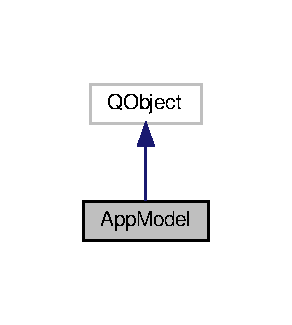
\includegraphics[width=140pt]{class_app_model__inherit__graph}
\end{center}
\end{figure}
\subsection*{Public Slots}
\begin{DoxyCompactItemize}
\item 
Q\+\_\+\+I\+N\+V\+O\+K\+A\+B\+LE void \hyperlink{class_app_model_a37e1da9d028779f7f0fc908e4c04fa76}{refresh\+Weather} ()
\begin{DoxyCompactList}\small\item\em \hyperlink{class_app_model_a37e1da9d028779f7f0fc908e4c04fa76}{App\+Model\+::refresh\+Weather} Access \href{http://api.openweathermap.org/data/2.5/weather}{\tt http\+://api.\+openweathermap.\+org/data/2.\+5/weather} site to get a specific city data Deals with connection errors. \end{DoxyCompactList}\end{DoxyCompactItemize}
\subsection*{Signals}
\begin{DoxyCompactItemize}
\item 
void \hyperlink{class_app_model_a574c2bd6f5c92ac9268107f8399989cb}{ready\+Changed} ()
\begin{DoxyCompactList}\small\item\em \mbox{[}3\mbox{]} \end{DoxyCompactList}\item 
void \hyperlink{class_app_model_af0007ee4da862433868baa5fdb31a3fe}{use\+Gps\+Changed} ()
\item 
void \hyperlink{class_app_model_a947db57e8c272bdb2420f3f273cd2e6a}{use\+Sensor\+Changed} ()
\item 
void \hyperlink{class_app_model_aeb28c7a57316aaf6295a943a65f60569}{city\+Changed} ()
\item 
void \hyperlink{class_app_model_a83e61455ed5672333b0db45f3f86417c}{weather\+Changed} ()
\end{DoxyCompactItemize}
\subsection*{Public Member Functions}
\begin{DoxyCompactItemize}
\item 
\hyperlink{class_app_model_affb3ea459bceb0650cdc810f3f5a2256}{App\+Model} (Q\+Object $\ast$parent=0)
\begin{DoxyCompactList}\small\item\em \mbox{[}0\mbox{]} \end{DoxyCompactList}\item 
\hyperlink{class_app_model_a67ab3004ccbe2822a8a0abb9fa96ace3}{$\sim$\+App\+Model} ()
\begin{DoxyCompactList}\small\item\em \mbox{[}1\mbox{]} \end{DoxyCompactList}\item 
bool \hyperlink{class_app_model_a3917fdc3dd8c97715991d9fd1a23abcc}{ready} () const
\item 
bool \hyperlink{class_app_model_a8ad68e982b0a307d9986ff538baedbd2}{has\+Source} () const
\item 
bool \hyperlink{class_app_model_a0e6e7506ba084133a6927d8c633ad699}{use\+Gps} () const
\item 
bool \hyperlink{class_app_model_a5b83f8c93976273d6e9f1664e62efe63}{use\+Sensor} () const
\item 
bool \hyperlink{class_app_model_aedeadab67d9bc5f5dfead369f66c3912}{has\+Valid\+City} () const
\item 
bool \hyperlink{class_app_model_a6ec5b34a1839a7141979709418174ad1}{has\+Valid\+Weather} () const
\item 
void \hyperlink{class_app_model_a81c3ffb3370837086366c9f70bb3d5eb}{set\+Use\+Gps} (bool value)
\item 
void \hyperlink{class_app_model_ac5fe590924b727724d9c686bb2552ed8}{had\+Error} (bool try\+Again)
\item 
void \hyperlink{class_app_model_ad1369130f74b4aabd0ac0d6b1b030014}{set\+Use\+Sensor} (bool value)
\item 
Q\+String \hyperlink{class_app_model_a093066c81b5fe2c1361df8fd19a21f51}{city} () const
\item 
void \hyperlink{class_app_model_ad0135d4a1551b6484ac28c434f861af5}{set\+City} (const Q\+String \&value)
\item 
\hyperlink{class_weather_data}{Weather\+Data} $\ast$ \hyperlink{class_app_model_a70a5bec8e359e4edbd16611efa96cf32}{weather} () const
\item 
Q\+Qml\+List\+Property$<$ \hyperlink{class_weather_data}{Weather\+Data} $>$ \hyperlink{class_app_model_aa9209b2390924841a009ab0d22b9a1b3}{forecast} () const
\end{DoxyCompactItemize}
\subsection*{Properties}
\begin{DoxyCompactItemize}
\item 
bool \hyperlink{class_app_model_a2af4f584bf701bff4546e889c16316d7}{ready}
\item 
bool \hyperlink{class_app_model_a2d25ce9151aea6a45cae797756a84445}{has\+Source}
\item 
bool \hyperlink{class_app_model_a98845ef5ffa3d9db0ee22aa3534b8608}{has\+Valid\+City}
\item 
bool \hyperlink{class_app_model_a493654987603c091935810e34e6b5c05}{has\+Valid\+Weather}
\item 
bool \hyperlink{class_app_model_aac827e2dce65eb299d4eec5ff4ab2155}{use\+Gps}
\item 
bool \hyperlink{class_app_model_ada296063fe2916580f532b639a546851}{use\+Sensor}
\item 
Q\+String \hyperlink{class_app_model_aa6915cabdaaf04805e00b5a2f75311e8}{city}
\item 
\hyperlink{class_weather_data}{Weather\+Data} \hyperlink{class_app_model_a72dfc16433c4ca50da689205e9db9298}{weather}
\item 
Q\+Qml\+List\+Property$<$ \hyperlink{class_weather_data}{Weather\+Data} $>$ \hyperlink{class_app_model_a3e45f56df91b1ad6d27c02c4ab1ad3c3}{forecast}
\end{DoxyCompactItemize}


\subsection{Detailed Description}
\mbox{[}2\mbox{]} 

\subsection{Constructor \& Destructor Documentation}
\mbox{\Hypertarget{class_app_model_affb3ea459bceb0650cdc810f3f5a2256}\label{class_app_model_affb3ea459bceb0650cdc810f3f5a2256}} 
\index{App\+Model@{App\+Model}!App\+Model@{App\+Model}}
\index{App\+Model@{App\+Model}!App\+Model@{App\+Model}}
\subsubsection{\texorpdfstring{App\+Model()}{AppModel()}}
{\footnotesize\ttfamily App\+Model\+::\+App\+Model (\begin{DoxyParamCaption}\item[{Q\+Object $\ast$}]{parent = {\ttfamily 0} }\end{DoxyParamCaption})\hspace{0.3cm}{\ttfamily [explicit]}}



\mbox{[}0\mbox{]} 

\mbox{[}0\mbox{]}

\mbox{[}1\mbox{]} \mbox{\Hypertarget{class_app_model_a67ab3004ccbe2822a8a0abb9fa96ace3}\label{class_app_model_a67ab3004ccbe2822a8a0abb9fa96ace3}} 
\index{App\+Model@{App\+Model}!````~App\+Model@{$\sim$\+App\+Model}}
\index{````~App\+Model@{$\sim$\+App\+Model}!App\+Model@{App\+Model}}
\subsubsection{\texorpdfstring{$\sim$\+App\+Model()}{~AppModel()}}
{\footnotesize\ttfamily App\+Model\+::$\sim$\+App\+Model (\begin{DoxyParamCaption}{ }\end{DoxyParamCaption})}



\mbox{[}1\mbox{]} 

Here is the call graph for this function\+:
\nopagebreak
\begin{figure}[H]
\begin{center}
\leavevmode
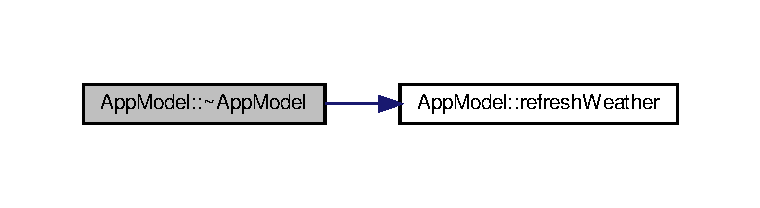
\includegraphics[width=350pt]{class_app_model_a67ab3004ccbe2822a8a0abb9fa96ace3_cgraph}
\end{center}
\end{figure}


\subsection{Member Function Documentation}
\mbox{\Hypertarget{class_app_model_a093066c81b5fe2c1361df8fd19a21f51}\label{class_app_model_a093066c81b5fe2c1361df8fd19a21f51}} 
\index{App\+Model@{App\+Model}!city@{city}}
\index{city@{city}!App\+Model@{App\+Model}}
\subsubsection{\texorpdfstring{city()}{city()}}
{\footnotesize\ttfamily Q\+String App\+Model\+::city (\begin{DoxyParamCaption}{ }\end{DoxyParamCaption}) const}

Here is the caller graph for this function\+:
\nopagebreak
\begin{figure}[H]
\begin{center}
\leavevmode
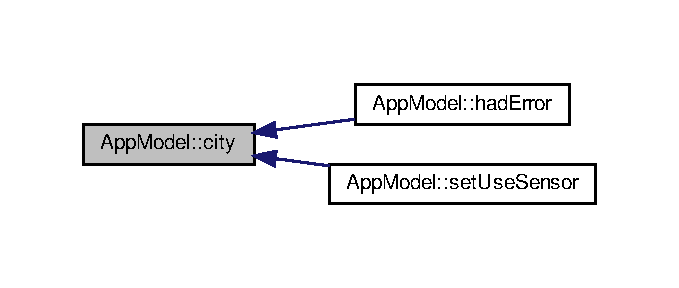
\includegraphics[width=326pt]{class_app_model_a093066c81b5fe2c1361df8fd19a21f51_icgraph}
\end{center}
\end{figure}
\mbox{\Hypertarget{class_app_model_aeb28c7a57316aaf6295a943a65f60569}\label{class_app_model_aeb28c7a57316aaf6295a943a65f60569}} 
\index{App\+Model@{App\+Model}!city\+Changed@{city\+Changed}}
\index{city\+Changed@{city\+Changed}!App\+Model@{App\+Model}}
\subsubsection{\texorpdfstring{city\+Changed}{cityChanged}}
{\footnotesize\ttfamily void App\+Model\+::city\+Changed (\begin{DoxyParamCaption}{ }\end{DoxyParamCaption})\hspace{0.3cm}{\ttfamily [signal]}}

Here is the caller graph for this function\+:
\nopagebreak
\begin{figure}[H]
\begin{center}
\leavevmode
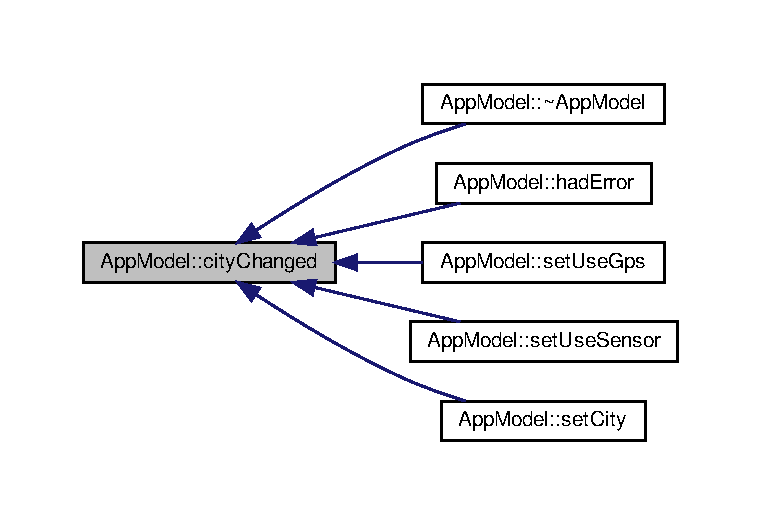
\includegraphics[width=350pt]{class_app_model_aeb28c7a57316aaf6295a943a65f60569_icgraph}
\end{center}
\end{figure}
\mbox{\Hypertarget{class_app_model_aa9209b2390924841a009ab0d22b9a1b3}\label{class_app_model_aa9209b2390924841a009ab0d22b9a1b3}} 
\index{App\+Model@{App\+Model}!forecast@{forecast}}
\index{forecast@{forecast}!App\+Model@{App\+Model}}
\subsubsection{\texorpdfstring{forecast()}{forecast()}}
{\footnotesize\ttfamily Q\+Qml\+List\+Property$<$\hyperlink{class_weather_data}{Weather\+Data}$>$ App\+Model\+::forecast (\begin{DoxyParamCaption}{ }\end{DoxyParamCaption}) const}

\mbox{\Hypertarget{class_app_model_ac5fe590924b727724d9c686bb2552ed8}\label{class_app_model_ac5fe590924b727724d9c686bb2552ed8}} 
\index{App\+Model@{App\+Model}!had\+Error@{had\+Error}}
\index{had\+Error@{had\+Error}!App\+Model@{App\+Model}}
\subsubsection{\texorpdfstring{had\+Error()}{hadError()}}
{\footnotesize\ttfamily void App\+Model\+::had\+Error (\begin{DoxyParamCaption}\item[{bool}]{try\+Again }\end{DoxyParamCaption})}

Manage time to wait before sending new request to get weather information before Here is the call graph for this function\+:
\nopagebreak
\begin{figure}[H]
\begin{center}
\leavevmode
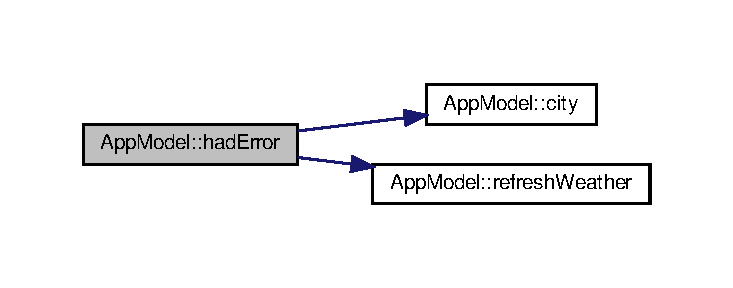
\includegraphics[width=350pt]{class_app_model_ac5fe590924b727724d9c686bb2552ed8_cgraph}
\end{center}
\end{figure}
\mbox{\Hypertarget{class_app_model_a8ad68e982b0a307d9986ff538baedbd2}\label{class_app_model_a8ad68e982b0a307d9986ff538baedbd2}} 
\index{App\+Model@{App\+Model}!has\+Source@{has\+Source}}
\index{has\+Source@{has\+Source}!App\+Model@{App\+Model}}
\subsubsection{\texorpdfstring{has\+Source()}{hasSource()}}
{\footnotesize\ttfamily bool App\+Model\+::has\+Source (\begin{DoxyParamCaption}{ }\end{DoxyParamCaption}) const}

\mbox{\Hypertarget{class_app_model_aedeadab67d9bc5f5dfead369f66c3912}\label{class_app_model_aedeadab67d9bc5f5dfead369f66c3912}} 
\index{App\+Model@{App\+Model}!has\+Valid\+City@{has\+Valid\+City}}
\index{has\+Valid\+City@{has\+Valid\+City}!App\+Model@{App\+Model}}
\subsubsection{\texorpdfstring{has\+Valid\+City()}{hasValidCity()}}
{\footnotesize\ttfamily bool App\+Model\+::has\+Valid\+City (\begin{DoxyParamCaption}{ }\end{DoxyParamCaption}) const}

\mbox{\Hypertarget{class_app_model_a6ec5b34a1839a7141979709418174ad1}\label{class_app_model_a6ec5b34a1839a7141979709418174ad1}} 
\index{App\+Model@{App\+Model}!has\+Valid\+Weather@{has\+Valid\+Weather}}
\index{has\+Valid\+Weather@{has\+Valid\+Weather}!App\+Model@{App\+Model}}
\subsubsection{\texorpdfstring{has\+Valid\+Weather()}{hasValidWeather()}}
{\footnotesize\ttfamily bool App\+Model\+::has\+Valid\+Weather (\begin{DoxyParamCaption}{ }\end{DoxyParamCaption}) const}

\mbox{\Hypertarget{class_app_model_a3917fdc3dd8c97715991d9fd1a23abcc}\label{class_app_model_a3917fdc3dd8c97715991d9fd1a23abcc}} 
\index{App\+Model@{App\+Model}!ready@{ready}}
\index{ready@{ready}!App\+Model@{App\+Model}}
\subsubsection{\texorpdfstring{ready()}{ready()}}
{\footnotesize\ttfamily bool App\+Model\+::ready (\begin{DoxyParamCaption}{ }\end{DoxyParamCaption}) const}

\mbox{\Hypertarget{class_app_model_a574c2bd6f5c92ac9268107f8399989cb}\label{class_app_model_a574c2bd6f5c92ac9268107f8399989cb}} 
\index{App\+Model@{App\+Model}!ready\+Changed@{ready\+Changed}}
\index{ready\+Changed@{ready\+Changed}!App\+Model@{App\+Model}}
\subsubsection{\texorpdfstring{ready\+Changed}{readyChanged}}
{\footnotesize\ttfamily void App\+Model\+::ready\+Changed (\begin{DoxyParamCaption}{ }\end{DoxyParamCaption})\hspace{0.3cm}{\ttfamily [signal]}}



\mbox{[}3\mbox{]} 

\mbox{\Hypertarget{class_app_model_a37e1da9d028779f7f0fc908e4c04fa76}\label{class_app_model_a37e1da9d028779f7f0fc908e4c04fa76}} 
\index{App\+Model@{App\+Model}!refresh\+Weather@{refresh\+Weather}}
\index{refresh\+Weather@{refresh\+Weather}!App\+Model@{App\+Model}}
\subsubsection{\texorpdfstring{refresh\+Weather}{refreshWeather}}
{\footnotesize\ttfamily void App\+Model\+::refresh\+Weather (\begin{DoxyParamCaption}{ }\end{DoxyParamCaption})\hspace{0.3cm}{\ttfamily [slot]}}



\hyperlink{class_app_model_a37e1da9d028779f7f0fc908e4c04fa76}{App\+Model\+::refresh\+Weather} Access \href{http://api.openweathermap.org/data/2.5/weather}{\tt http\+://api.\+openweathermap.\+org/data/2.\+5/weather} site to get a specific city data Deals with connection errors. 

Here is the caller graph for this function\+:
\nopagebreak
\begin{figure}[H]
\begin{center}
\leavevmode
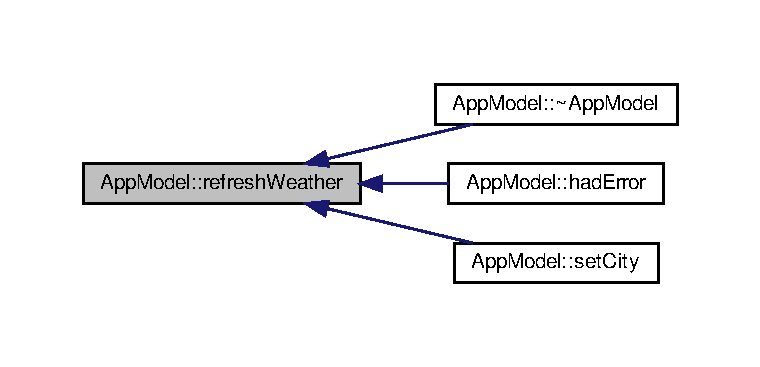
\includegraphics[width=350pt]{class_app_model_a37e1da9d028779f7f0fc908e4c04fa76_icgraph}
\end{center}
\end{figure}
\mbox{\Hypertarget{class_app_model_ad0135d4a1551b6484ac28c434f861af5}\label{class_app_model_ad0135d4a1551b6484ac28c434f861af5}} 
\index{App\+Model@{App\+Model}!set\+City@{set\+City}}
\index{set\+City@{set\+City}!App\+Model@{App\+Model}}
\subsubsection{\texorpdfstring{set\+City()}{setCity()}}
{\footnotesize\ttfamily void App\+Model\+::set\+City (\begin{DoxyParamCaption}\item[{const Q\+String \&}]{value }\end{DoxyParamCaption})}

Here is the call graph for this function\+:
\nopagebreak
\begin{figure}[H]
\begin{center}
\leavevmode
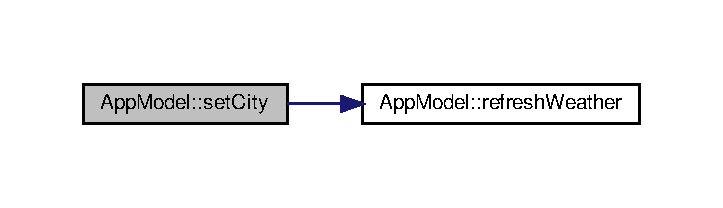
\includegraphics[width=347pt]{class_app_model_ad0135d4a1551b6484ac28c434f861af5_cgraph}
\end{center}
\end{figure}
\mbox{\Hypertarget{class_app_model_a81c3ffb3370837086366c9f70bb3d5eb}\label{class_app_model_a81c3ffb3370837086366c9f70bb3d5eb}} 
\index{App\+Model@{App\+Model}!set\+Use\+Gps@{set\+Use\+Gps}}
\index{set\+Use\+Gps@{set\+Use\+Gps}!App\+Model@{App\+Model}}
\subsubsection{\texorpdfstring{set\+Use\+Gps()}{setUseGps()}}
{\footnotesize\ttfamily void App\+Model\+::set\+Use\+Gps (\begin{DoxyParamCaption}\item[{bool}]{value }\end{DoxyParamCaption})}

Here is the call graph for this function\+:
\nopagebreak
\begin{figure}[H]
\begin{center}
\leavevmode
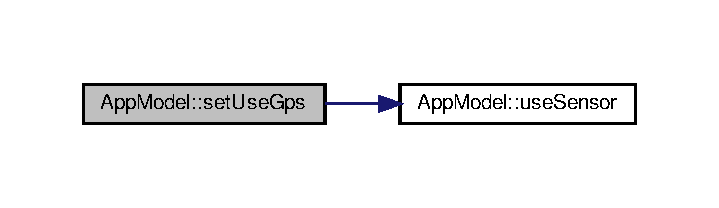
\includegraphics[width=345pt]{class_app_model_a81c3ffb3370837086366c9f70bb3d5eb_cgraph}
\end{center}
\end{figure}
\mbox{\Hypertarget{class_app_model_ad1369130f74b4aabd0ac0d6b1b030014}\label{class_app_model_ad1369130f74b4aabd0ac0d6b1b030014}} 
\index{App\+Model@{App\+Model}!set\+Use\+Sensor@{set\+Use\+Sensor}}
\index{set\+Use\+Sensor@{set\+Use\+Sensor}!App\+Model@{App\+Model}}
\subsubsection{\texorpdfstring{set\+Use\+Sensor()}{setUseSensor()}}
{\footnotesize\ttfamily void App\+Model\+::set\+Use\+Sensor (\begin{DoxyParamCaption}\item[{bool}]{value }\end{DoxyParamCaption})}

Here is the call graph for this function\+:
\nopagebreak
\begin{figure}[H]
\begin{center}
\leavevmode
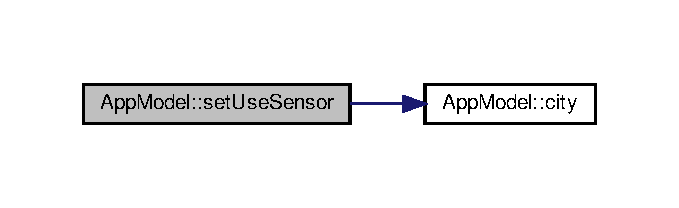
\includegraphics[width=326pt]{class_app_model_ad1369130f74b4aabd0ac0d6b1b030014_cgraph}
\end{center}
\end{figure}
\mbox{\Hypertarget{class_app_model_a0e6e7506ba084133a6927d8c633ad699}\label{class_app_model_a0e6e7506ba084133a6927d8c633ad699}} 
\index{App\+Model@{App\+Model}!use\+Gps@{use\+Gps}}
\index{use\+Gps@{use\+Gps}!App\+Model@{App\+Model}}
\subsubsection{\texorpdfstring{use\+Gps()}{useGps()}}
{\footnotesize\ttfamily bool App\+Model\+::use\+Gps (\begin{DoxyParamCaption}{ }\end{DoxyParamCaption}) const}

\mbox{\Hypertarget{class_app_model_af0007ee4da862433868baa5fdb31a3fe}\label{class_app_model_af0007ee4da862433868baa5fdb31a3fe}} 
\index{App\+Model@{App\+Model}!use\+Gps\+Changed@{use\+Gps\+Changed}}
\index{use\+Gps\+Changed@{use\+Gps\+Changed}!App\+Model@{App\+Model}}
\subsubsection{\texorpdfstring{use\+Gps\+Changed}{useGpsChanged}}
{\footnotesize\ttfamily void App\+Model\+::use\+Gps\+Changed (\begin{DoxyParamCaption}{ }\end{DoxyParamCaption})\hspace{0.3cm}{\ttfamily [signal]}}

Here is the caller graph for this function\+:
\nopagebreak
\begin{figure}[H]
\begin{center}
\leavevmode
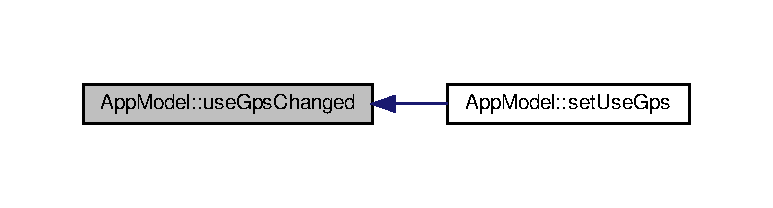
\includegraphics[width=350pt]{class_app_model_af0007ee4da862433868baa5fdb31a3fe_icgraph}
\end{center}
\end{figure}
\mbox{\Hypertarget{class_app_model_a5b83f8c93976273d6e9f1664e62efe63}\label{class_app_model_a5b83f8c93976273d6e9f1664e62efe63}} 
\index{App\+Model@{App\+Model}!use\+Sensor@{use\+Sensor}}
\index{use\+Sensor@{use\+Sensor}!App\+Model@{App\+Model}}
\subsubsection{\texorpdfstring{use\+Sensor()}{useSensor()}}
{\footnotesize\ttfamily bool App\+Model\+::use\+Sensor (\begin{DoxyParamCaption}{ }\end{DoxyParamCaption}) const}

Here is the caller graph for this function\+:
\nopagebreak
\begin{figure}[H]
\begin{center}
\leavevmode
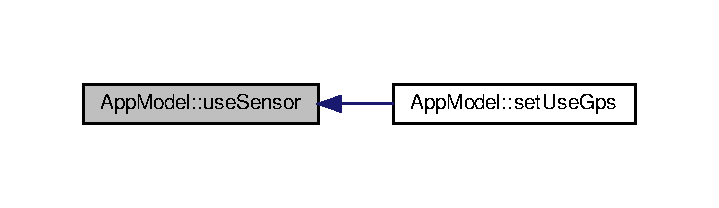
\includegraphics[width=345pt]{class_app_model_a5b83f8c93976273d6e9f1664e62efe63_icgraph}
\end{center}
\end{figure}
\mbox{\Hypertarget{class_app_model_a947db57e8c272bdb2420f3f273cd2e6a}\label{class_app_model_a947db57e8c272bdb2420f3f273cd2e6a}} 
\index{App\+Model@{App\+Model}!use\+Sensor\+Changed@{use\+Sensor\+Changed}}
\index{use\+Sensor\+Changed@{use\+Sensor\+Changed}!App\+Model@{App\+Model}}
\subsubsection{\texorpdfstring{use\+Sensor\+Changed}{useSensorChanged}}
{\footnotesize\ttfamily void App\+Model\+::use\+Sensor\+Changed (\begin{DoxyParamCaption}{ }\end{DoxyParamCaption})\hspace{0.3cm}{\ttfamily [signal]}}

Here is the caller graph for this function\+:
\nopagebreak
\begin{figure}[H]
\begin{center}
\leavevmode
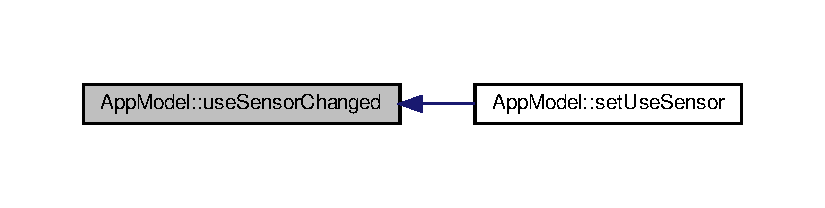
\includegraphics[width=350pt]{class_app_model_a947db57e8c272bdb2420f3f273cd2e6a_icgraph}
\end{center}
\end{figure}
\mbox{\Hypertarget{class_app_model_a70a5bec8e359e4edbd16611efa96cf32}\label{class_app_model_a70a5bec8e359e4edbd16611efa96cf32}} 
\index{App\+Model@{App\+Model}!weather@{weather}}
\index{weather@{weather}!App\+Model@{App\+Model}}
\subsubsection{\texorpdfstring{weather()}{weather()}}
{\footnotesize\ttfamily \hyperlink{class_weather_data}{Weather\+Data}$\ast$ App\+Model\+::weather (\begin{DoxyParamCaption}{ }\end{DoxyParamCaption}) const}

\mbox{\Hypertarget{class_app_model_a83e61455ed5672333b0db45f3f86417c}\label{class_app_model_a83e61455ed5672333b0db45f3f86417c}} 
\index{App\+Model@{App\+Model}!weather\+Changed@{weather\+Changed}}
\index{weather\+Changed@{weather\+Changed}!App\+Model@{App\+Model}}
\subsubsection{\texorpdfstring{weather\+Changed}{weatherChanged}}
{\footnotesize\ttfamily void App\+Model\+::weather\+Changed (\begin{DoxyParamCaption}{ }\end{DoxyParamCaption})\hspace{0.3cm}{\ttfamily [signal]}}

Here is the caller graph for this function\+:
\nopagebreak
\begin{figure}[H]
\begin{center}
\leavevmode
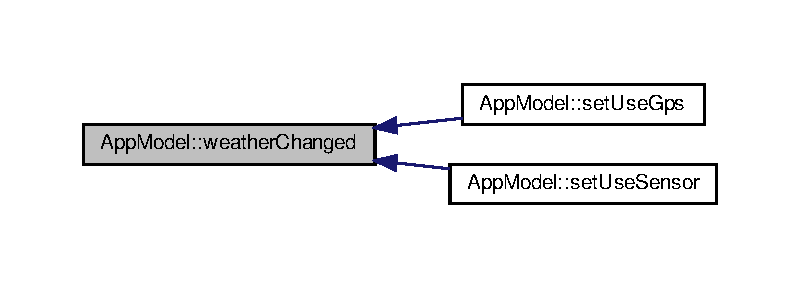
\includegraphics[width=350pt]{class_app_model_a83e61455ed5672333b0db45f3f86417c_icgraph}
\end{center}
\end{figure}


\subsection{Property Documentation}
\mbox{\Hypertarget{class_app_model_aa6915cabdaaf04805e00b5a2f75311e8}\label{class_app_model_aa6915cabdaaf04805e00b5a2f75311e8}} 
\index{App\+Model@{App\+Model}!city@{city}}
\index{city@{city}!App\+Model@{App\+Model}}
\subsubsection{\texorpdfstring{city}{city}}
{\footnotesize\ttfamily Q\+String App\+Model\+::city\hspace{0.3cm}{\ttfamily [read]}, {\ttfamily [write]}}

\mbox{\Hypertarget{class_app_model_a3e45f56df91b1ad6d27c02c4ab1ad3c3}\label{class_app_model_a3e45f56df91b1ad6d27c02c4ab1ad3c3}} 
\index{App\+Model@{App\+Model}!forecast@{forecast}}
\index{forecast@{forecast}!App\+Model@{App\+Model}}
\subsubsection{\texorpdfstring{forecast}{forecast}}
{\footnotesize\ttfamily Q\+Qml\+List\+Property$<$ \hyperlink{class_weather_data}{Weather\+Data} $>$ App\+Model\+::forecast\hspace{0.3cm}{\ttfamily [read]}}

\mbox{\Hypertarget{class_app_model_a2d25ce9151aea6a45cae797756a84445}\label{class_app_model_a2d25ce9151aea6a45cae797756a84445}} 
\index{App\+Model@{App\+Model}!has\+Source@{has\+Source}}
\index{has\+Source@{has\+Source}!App\+Model@{App\+Model}}
\subsubsection{\texorpdfstring{has\+Source}{hasSource}}
{\footnotesize\ttfamily bool App\+Model\+::has\+Source\hspace{0.3cm}{\ttfamily [read]}}

\mbox{\Hypertarget{class_app_model_a98845ef5ffa3d9db0ee22aa3534b8608}\label{class_app_model_a98845ef5ffa3d9db0ee22aa3534b8608}} 
\index{App\+Model@{App\+Model}!has\+Valid\+City@{has\+Valid\+City}}
\index{has\+Valid\+City@{has\+Valid\+City}!App\+Model@{App\+Model}}
\subsubsection{\texorpdfstring{has\+Valid\+City}{hasValidCity}}
{\footnotesize\ttfamily bool App\+Model\+::has\+Valid\+City\hspace{0.3cm}{\ttfamily [read]}}

\mbox{\Hypertarget{class_app_model_a493654987603c091935810e34e6b5c05}\label{class_app_model_a493654987603c091935810e34e6b5c05}} 
\index{App\+Model@{App\+Model}!has\+Valid\+Weather@{has\+Valid\+Weather}}
\index{has\+Valid\+Weather@{has\+Valid\+Weather}!App\+Model@{App\+Model}}
\subsubsection{\texorpdfstring{has\+Valid\+Weather}{hasValidWeather}}
{\footnotesize\ttfamily bool App\+Model\+::has\+Valid\+Weather\hspace{0.3cm}{\ttfamily [read]}}

\mbox{\Hypertarget{class_app_model_a2af4f584bf701bff4546e889c16316d7}\label{class_app_model_a2af4f584bf701bff4546e889c16316d7}} 
\index{App\+Model@{App\+Model}!ready@{ready}}
\index{ready@{ready}!App\+Model@{App\+Model}}
\subsubsection{\texorpdfstring{ready}{ready}}
{\footnotesize\ttfamily bool App\+Model\+::ready\hspace{0.3cm}{\ttfamily [read]}}

\mbox{\Hypertarget{class_app_model_aac827e2dce65eb299d4eec5ff4ab2155}\label{class_app_model_aac827e2dce65eb299d4eec5ff4ab2155}} 
\index{App\+Model@{App\+Model}!use\+Gps@{use\+Gps}}
\index{use\+Gps@{use\+Gps}!App\+Model@{App\+Model}}
\subsubsection{\texorpdfstring{use\+Gps}{useGps}}
{\footnotesize\ttfamily bool App\+Model\+::use\+Gps\hspace{0.3cm}{\ttfamily [read]}, {\ttfamily [write]}}

\mbox{\Hypertarget{class_app_model_ada296063fe2916580f532b639a546851}\label{class_app_model_ada296063fe2916580f532b639a546851}} 
\index{App\+Model@{App\+Model}!use\+Sensor@{use\+Sensor}}
\index{use\+Sensor@{use\+Sensor}!App\+Model@{App\+Model}}
\subsubsection{\texorpdfstring{use\+Sensor}{useSensor}}
{\footnotesize\ttfamily bool App\+Model\+::use\+Sensor\hspace{0.3cm}{\ttfamily [read]}, {\ttfamily [write]}}

\mbox{\Hypertarget{class_app_model_a72dfc16433c4ca50da689205e9db9298}\label{class_app_model_a72dfc16433c4ca50da689205e9db9298}} 
\index{App\+Model@{App\+Model}!weather@{weather}}
\index{weather@{weather}!App\+Model@{App\+Model}}
\subsubsection{\texorpdfstring{weather}{weather}}
{\footnotesize\ttfamily \hyperlink{class_weather_data}{Weather\+Data} $\ast$ App\+Model\+::weather\hspace{0.3cm}{\ttfamily [read]}}



The documentation for this class was generated from the following files\+:\begin{DoxyCompactItemize}
\item 
/home/jerome/projects/\+Weather\+Checking\+Rpi/weathercheckingrpi/\hyperlink{appmodel_8h}{appmodel.\+h}\item 
/home/jerome/projects/\+Weather\+Checking\+Rpi/weathercheckingrpi/\hyperlink{appmodel_8cpp}{appmodel.\+cpp}\end{DoxyCompactItemize}

\hypertarget{class_app_model_private}{}\section{App\+Model\+Private Class Reference}
\label{class_app_model_private}\index{App\+Model\+Private@{App\+Model\+Private}}


Collaboration diagram for App\+Model\+Private\+:
\nopagebreak
\begin{figure}[H]
\begin{center}
\leavevmode
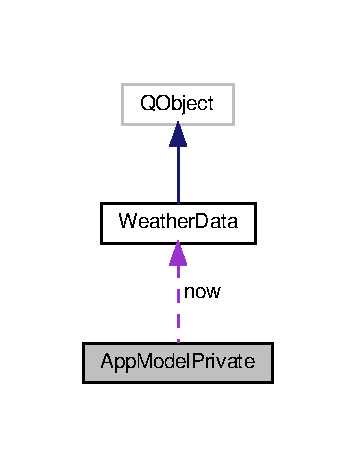
\includegraphics[width=171pt]{class_app_model_private__coll__graph}
\end{center}
\end{figure}
\subsection*{Public Member Functions}
\begin{DoxyCompactItemize}
\item 
\hyperlink{class_app_model_private_ac7e4e160306c7ff9c771d2dd34c243ac}{App\+Model\+Private} ()
\end{DoxyCompactItemize}
\subsection*{Public Attributes}
\begin{DoxyCompactItemize}
\item 
\hyperlink{class_weather_data}{Weather\+Data} \hyperlink{class_app_model_private_adacce6c96a2a7b0b825586a63a15bcac}{now}
\item 
bool \hyperlink{class_app_model_private_ab0434f387adadf9ed65183496fe80f77}{ready}
\item 
Q\+Timer \hyperlink{class_app_model_private_ad073c8bcf6739fd658009860e12aa72c}{request\+New\+Weather\+Timer}
\end{DoxyCompactItemize}


\subsection{Constructor \& Destructor Documentation}
\mbox{\Hypertarget{class_app_model_private_ac7e4e160306c7ff9c771d2dd34c243ac}\label{class_app_model_private_ac7e4e160306c7ff9c771d2dd34c243ac}} 
\index{App\+Model\+Private@{App\+Model\+Private}!App\+Model\+Private@{App\+Model\+Private}}
\index{App\+Model\+Private@{App\+Model\+Private}!App\+Model\+Private@{App\+Model\+Private}}
\subsubsection{\texorpdfstring{App\+Model\+Private()}{AppModelPrivate()}}
{\footnotesize\ttfamily App\+Model\+Private\+::\+App\+Model\+Private (\begin{DoxyParamCaption}{ }\end{DoxyParamCaption})\hspace{0.3cm}{\ttfamily [inline]}}



\subsection{Member Data Documentation}
\mbox{\Hypertarget{class_app_model_private_adacce6c96a2a7b0b825586a63a15bcac}\label{class_app_model_private_adacce6c96a2a7b0b825586a63a15bcac}} 
\index{App\+Model\+Private@{App\+Model\+Private}!now@{now}}
\index{now@{now}!App\+Model\+Private@{App\+Model\+Private}}
\subsubsection{\texorpdfstring{now}{now}}
{\footnotesize\ttfamily \hyperlink{class_weather_data}{Weather\+Data} App\+Model\+Private\+::now}

\mbox{\Hypertarget{class_app_model_private_ab0434f387adadf9ed65183496fe80f77}\label{class_app_model_private_ab0434f387adadf9ed65183496fe80f77}} 
\index{App\+Model\+Private@{App\+Model\+Private}!ready@{ready}}
\index{ready@{ready}!App\+Model\+Private@{App\+Model\+Private}}
\subsubsection{\texorpdfstring{ready}{ready}}
{\footnotesize\ttfamily bool App\+Model\+Private\+::ready}

\mbox{\Hypertarget{class_app_model_private_ad073c8bcf6739fd658009860e12aa72c}\label{class_app_model_private_ad073c8bcf6739fd658009860e12aa72c}} 
\index{App\+Model\+Private@{App\+Model\+Private}!request\+New\+Weather\+Timer@{request\+New\+Weather\+Timer}}
\index{request\+New\+Weather\+Timer@{request\+New\+Weather\+Timer}!App\+Model\+Private@{App\+Model\+Private}}
\subsubsection{\texorpdfstring{request\+New\+Weather\+Timer}{requestNewWeatherTimer}}
{\footnotesize\ttfamily Q\+Timer App\+Model\+Private\+::request\+New\+Weather\+Timer}



The documentation for this class was generated from the following file\+:\begin{DoxyCompactItemize}
\item 
\hyperlink{appmodel_8cpp}{appmodel.\+cpp}\end{DoxyCompactItemize}

\hypertarget{structbme280__calib__data}{}\section{bme280\+\_\+calib\+\_\+data Struct Reference}
\label{structbme280__calib__data}\index{bme280\+\_\+calib\+\_\+data@{bme280\+\_\+calib\+\_\+data}}


Calibration data.  




{\ttfamily \#include $<$bme280\+\_\+defs.\+h$>$}

\subsection*{Public Attributes}
\textbf{ }\par
\begin{DoxyCompactItemize}
\item 
uint16\+\_\+t \hyperlink{structbme280__calib__data_af8eb813b4a350b19596105013792aee8}{dig\+\_\+\+T1}
\item 
int16\+\_\+t \hyperlink{structbme280__calib__data_a608c0112ccb3fdc3c11f1e174cdbde1b}{dig\+\_\+\+T2}
\item 
int16\+\_\+t \hyperlink{structbme280__calib__data_af04a21f46f9244b879ad16af5a40ebb2}{dig\+\_\+\+T3}
\item 
uint16\+\_\+t \hyperlink{structbme280__calib__data_aa2a4a84a415069af6292d92fa2517c18}{dig\+\_\+\+P1}
\item 
int16\+\_\+t \hyperlink{structbme280__calib__data_a13ddffe344b00ae3230f5412019c25c7}{dig\+\_\+\+P2}
\item 
int16\+\_\+t \hyperlink{structbme280__calib__data_a8e86eee62639bef1ded9f51b6c863577}{dig\+\_\+\+P3}
\item 
int16\+\_\+t \hyperlink{structbme280__calib__data_abd53f31d52c16118691b65a59f51e388}{dig\+\_\+\+P4}
\item 
int16\+\_\+t \hyperlink{structbme280__calib__data_a5583773f96cdaf8ccdd20412082d8542}{dig\+\_\+\+P5}
\item 
int16\+\_\+t \hyperlink{structbme280__calib__data_aa5781cae586a4b1ed76ad78050fec41a}{dig\+\_\+\+P6}
\item 
int16\+\_\+t \hyperlink{structbme280__calib__data_a647f5cb10618b453ecd9b8819068ad13}{dig\+\_\+\+P7}
\item 
int16\+\_\+t \hyperlink{structbme280__calib__data_a405be361198254a2522797bd38f7a2a0}{dig\+\_\+\+P8}
\item 
int16\+\_\+t \hyperlink{structbme280__calib__data_aaba752b373db185367a51c481bae6f75}{dig\+\_\+\+P9}
\item 
uint8\+\_\+t \hyperlink{structbme280__calib__data_aa6521d4105f928a3734361923ded1402}{dig\+\_\+\+H1}
\item 
int16\+\_\+t \hyperlink{structbme280__calib__data_a129f0a99b6fa997aff11d1e66800f762}{dig\+\_\+\+H2}
\item 
uint8\+\_\+t \hyperlink{structbme280__calib__data_a567370a48166d5c44493f0bf172fbaad}{dig\+\_\+\+H3}
\item 
int16\+\_\+t \hyperlink{structbme280__calib__data_a2b1fb6cbf75cae79fa5ea43d8e5eb6f7}{dig\+\_\+\+H4}
\item 
int16\+\_\+t \hyperlink{structbme280__calib__data_a36cff966ad8a2777b773b5da5930830b}{dig\+\_\+\+H5}
\item 
int8\+\_\+t \hyperlink{structbme280__calib__data_a9aab678b157796957cb0819fa3027599}{dig\+\_\+\+H6}
\item 
int32\+\_\+t \hyperlink{structbme280__calib__data_a035b8d8756456820ec82f26a2cf62ffa}{t\+\_\+fine}
\end{DoxyCompactItemize}



\subsection{Detailed Description}
Calibration data. 

\subsection{Member Data Documentation}
\mbox{\Hypertarget{structbme280__calib__data_aa6521d4105f928a3734361923ded1402}\label{structbme280__calib__data_aa6521d4105f928a3734361923ded1402}} 
\index{bme280\+\_\+calib\+\_\+data@{bme280\+\_\+calib\+\_\+data}!dig\+\_\+\+H1@{dig\+\_\+\+H1}}
\index{dig\+\_\+\+H1@{dig\+\_\+\+H1}!bme280\+\_\+calib\+\_\+data@{bme280\+\_\+calib\+\_\+data}}
\subsubsection{\texorpdfstring{dig\+\_\+\+H1}{dig\_H1}}
{\footnotesize\ttfamily uint8\+\_\+t bme280\+\_\+calib\+\_\+data\+::dig\+\_\+\+H1}

\mbox{\Hypertarget{structbme280__calib__data_a129f0a99b6fa997aff11d1e66800f762}\label{structbme280__calib__data_a129f0a99b6fa997aff11d1e66800f762}} 
\index{bme280\+\_\+calib\+\_\+data@{bme280\+\_\+calib\+\_\+data}!dig\+\_\+\+H2@{dig\+\_\+\+H2}}
\index{dig\+\_\+\+H2@{dig\+\_\+\+H2}!bme280\+\_\+calib\+\_\+data@{bme280\+\_\+calib\+\_\+data}}
\subsubsection{\texorpdfstring{dig\+\_\+\+H2}{dig\_H2}}
{\footnotesize\ttfamily int16\+\_\+t bme280\+\_\+calib\+\_\+data\+::dig\+\_\+\+H2}

\mbox{\Hypertarget{structbme280__calib__data_a567370a48166d5c44493f0bf172fbaad}\label{structbme280__calib__data_a567370a48166d5c44493f0bf172fbaad}} 
\index{bme280\+\_\+calib\+\_\+data@{bme280\+\_\+calib\+\_\+data}!dig\+\_\+\+H3@{dig\+\_\+\+H3}}
\index{dig\+\_\+\+H3@{dig\+\_\+\+H3}!bme280\+\_\+calib\+\_\+data@{bme280\+\_\+calib\+\_\+data}}
\subsubsection{\texorpdfstring{dig\+\_\+\+H3}{dig\_H3}}
{\footnotesize\ttfamily uint8\+\_\+t bme280\+\_\+calib\+\_\+data\+::dig\+\_\+\+H3}

\mbox{\Hypertarget{structbme280__calib__data_a2b1fb6cbf75cae79fa5ea43d8e5eb6f7}\label{structbme280__calib__data_a2b1fb6cbf75cae79fa5ea43d8e5eb6f7}} 
\index{bme280\+\_\+calib\+\_\+data@{bme280\+\_\+calib\+\_\+data}!dig\+\_\+\+H4@{dig\+\_\+\+H4}}
\index{dig\+\_\+\+H4@{dig\+\_\+\+H4}!bme280\+\_\+calib\+\_\+data@{bme280\+\_\+calib\+\_\+data}}
\subsubsection{\texorpdfstring{dig\+\_\+\+H4}{dig\_H4}}
{\footnotesize\ttfamily int16\+\_\+t bme280\+\_\+calib\+\_\+data\+::dig\+\_\+\+H4}

\mbox{\Hypertarget{structbme280__calib__data_a36cff966ad8a2777b773b5da5930830b}\label{structbme280__calib__data_a36cff966ad8a2777b773b5da5930830b}} 
\index{bme280\+\_\+calib\+\_\+data@{bme280\+\_\+calib\+\_\+data}!dig\+\_\+\+H5@{dig\+\_\+\+H5}}
\index{dig\+\_\+\+H5@{dig\+\_\+\+H5}!bme280\+\_\+calib\+\_\+data@{bme280\+\_\+calib\+\_\+data}}
\subsubsection{\texorpdfstring{dig\+\_\+\+H5}{dig\_H5}}
{\footnotesize\ttfamily int16\+\_\+t bme280\+\_\+calib\+\_\+data\+::dig\+\_\+\+H5}

\mbox{\Hypertarget{structbme280__calib__data_a9aab678b157796957cb0819fa3027599}\label{structbme280__calib__data_a9aab678b157796957cb0819fa3027599}} 
\index{bme280\+\_\+calib\+\_\+data@{bme280\+\_\+calib\+\_\+data}!dig\+\_\+\+H6@{dig\+\_\+\+H6}}
\index{dig\+\_\+\+H6@{dig\+\_\+\+H6}!bme280\+\_\+calib\+\_\+data@{bme280\+\_\+calib\+\_\+data}}
\subsubsection{\texorpdfstring{dig\+\_\+\+H6}{dig\_H6}}
{\footnotesize\ttfamily int8\+\_\+t bme280\+\_\+calib\+\_\+data\+::dig\+\_\+\+H6}

\mbox{\Hypertarget{structbme280__calib__data_aa2a4a84a415069af6292d92fa2517c18}\label{structbme280__calib__data_aa2a4a84a415069af6292d92fa2517c18}} 
\index{bme280\+\_\+calib\+\_\+data@{bme280\+\_\+calib\+\_\+data}!dig\+\_\+\+P1@{dig\+\_\+\+P1}}
\index{dig\+\_\+\+P1@{dig\+\_\+\+P1}!bme280\+\_\+calib\+\_\+data@{bme280\+\_\+calib\+\_\+data}}
\subsubsection{\texorpdfstring{dig\+\_\+\+P1}{dig\_P1}}
{\footnotesize\ttfamily uint16\+\_\+t bme280\+\_\+calib\+\_\+data\+::dig\+\_\+\+P1}

\mbox{\Hypertarget{structbme280__calib__data_a13ddffe344b00ae3230f5412019c25c7}\label{structbme280__calib__data_a13ddffe344b00ae3230f5412019c25c7}} 
\index{bme280\+\_\+calib\+\_\+data@{bme280\+\_\+calib\+\_\+data}!dig\+\_\+\+P2@{dig\+\_\+\+P2}}
\index{dig\+\_\+\+P2@{dig\+\_\+\+P2}!bme280\+\_\+calib\+\_\+data@{bme280\+\_\+calib\+\_\+data}}
\subsubsection{\texorpdfstring{dig\+\_\+\+P2}{dig\_P2}}
{\footnotesize\ttfamily int16\+\_\+t bme280\+\_\+calib\+\_\+data\+::dig\+\_\+\+P2}

\mbox{\Hypertarget{structbme280__calib__data_a8e86eee62639bef1ded9f51b6c863577}\label{structbme280__calib__data_a8e86eee62639bef1ded9f51b6c863577}} 
\index{bme280\+\_\+calib\+\_\+data@{bme280\+\_\+calib\+\_\+data}!dig\+\_\+\+P3@{dig\+\_\+\+P3}}
\index{dig\+\_\+\+P3@{dig\+\_\+\+P3}!bme280\+\_\+calib\+\_\+data@{bme280\+\_\+calib\+\_\+data}}
\subsubsection{\texorpdfstring{dig\+\_\+\+P3}{dig\_P3}}
{\footnotesize\ttfamily int16\+\_\+t bme280\+\_\+calib\+\_\+data\+::dig\+\_\+\+P3}

\mbox{\Hypertarget{structbme280__calib__data_abd53f31d52c16118691b65a59f51e388}\label{structbme280__calib__data_abd53f31d52c16118691b65a59f51e388}} 
\index{bme280\+\_\+calib\+\_\+data@{bme280\+\_\+calib\+\_\+data}!dig\+\_\+\+P4@{dig\+\_\+\+P4}}
\index{dig\+\_\+\+P4@{dig\+\_\+\+P4}!bme280\+\_\+calib\+\_\+data@{bme280\+\_\+calib\+\_\+data}}
\subsubsection{\texorpdfstring{dig\+\_\+\+P4}{dig\_P4}}
{\footnotesize\ttfamily int16\+\_\+t bme280\+\_\+calib\+\_\+data\+::dig\+\_\+\+P4}

\mbox{\Hypertarget{structbme280__calib__data_a5583773f96cdaf8ccdd20412082d8542}\label{structbme280__calib__data_a5583773f96cdaf8ccdd20412082d8542}} 
\index{bme280\+\_\+calib\+\_\+data@{bme280\+\_\+calib\+\_\+data}!dig\+\_\+\+P5@{dig\+\_\+\+P5}}
\index{dig\+\_\+\+P5@{dig\+\_\+\+P5}!bme280\+\_\+calib\+\_\+data@{bme280\+\_\+calib\+\_\+data}}
\subsubsection{\texorpdfstring{dig\+\_\+\+P5}{dig\_P5}}
{\footnotesize\ttfamily int16\+\_\+t bme280\+\_\+calib\+\_\+data\+::dig\+\_\+\+P5}

\mbox{\Hypertarget{structbme280__calib__data_aa5781cae586a4b1ed76ad78050fec41a}\label{structbme280__calib__data_aa5781cae586a4b1ed76ad78050fec41a}} 
\index{bme280\+\_\+calib\+\_\+data@{bme280\+\_\+calib\+\_\+data}!dig\+\_\+\+P6@{dig\+\_\+\+P6}}
\index{dig\+\_\+\+P6@{dig\+\_\+\+P6}!bme280\+\_\+calib\+\_\+data@{bme280\+\_\+calib\+\_\+data}}
\subsubsection{\texorpdfstring{dig\+\_\+\+P6}{dig\_P6}}
{\footnotesize\ttfamily int16\+\_\+t bme280\+\_\+calib\+\_\+data\+::dig\+\_\+\+P6}

\mbox{\Hypertarget{structbme280__calib__data_a647f5cb10618b453ecd9b8819068ad13}\label{structbme280__calib__data_a647f5cb10618b453ecd9b8819068ad13}} 
\index{bme280\+\_\+calib\+\_\+data@{bme280\+\_\+calib\+\_\+data}!dig\+\_\+\+P7@{dig\+\_\+\+P7}}
\index{dig\+\_\+\+P7@{dig\+\_\+\+P7}!bme280\+\_\+calib\+\_\+data@{bme280\+\_\+calib\+\_\+data}}
\subsubsection{\texorpdfstring{dig\+\_\+\+P7}{dig\_P7}}
{\footnotesize\ttfamily int16\+\_\+t bme280\+\_\+calib\+\_\+data\+::dig\+\_\+\+P7}

\mbox{\Hypertarget{structbme280__calib__data_a405be361198254a2522797bd38f7a2a0}\label{structbme280__calib__data_a405be361198254a2522797bd38f7a2a0}} 
\index{bme280\+\_\+calib\+\_\+data@{bme280\+\_\+calib\+\_\+data}!dig\+\_\+\+P8@{dig\+\_\+\+P8}}
\index{dig\+\_\+\+P8@{dig\+\_\+\+P8}!bme280\+\_\+calib\+\_\+data@{bme280\+\_\+calib\+\_\+data}}
\subsubsection{\texorpdfstring{dig\+\_\+\+P8}{dig\_P8}}
{\footnotesize\ttfamily int16\+\_\+t bme280\+\_\+calib\+\_\+data\+::dig\+\_\+\+P8}

\mbox{\Hypertarget{structbme280__calib__data_aaba752b373db185367a51c481bae6f75}\label{structbme280__calib__data_aaba752b373db185367a51c481bae6f75}} 
\index{bme280\+\_\+calib\+\_\+data@{bme280\+\_\+calib\+\_\+data}!dig\+\_\+\+P9@{dig\+\_\+\+P9}}
\index{dig\+\_\+\+P9@{dig\+\_\+\+P9}!bme280\+\_\+calib\+\_\+data@{bme280\+\_\+calib\+\_\+data}}
\subsubsection{\texorpdfstring{dig\+\_\+\+P9}{dig\_P9}}
{\footnotesize\ttfamily int16\+\_\+t bme280\+\_\+calib\+\_\+data\+::dig\+\_\+\+P9}

\mbox{\Hypertarget{structbme280__calib__data_af8eb813b4a350b19596105013792aee8}\label{structbme280__calib__data_af8eb813b4a350b19596105013792aee8}} 
\index{bme280\+\_\+calib\+\_\+data@{bme280\+\_\+calib\+\_\+data}!dig\+\_\+\+T1@{dig\+\_\+\+T1}}
\index{dig\+\_\+\+T1@{dig\+\_\+\+T1}!bme280\+\_\+calib\+\_\+data@{bme280\+\_\+calib\+\_\+data}}
\subsubsection{\texorpdfstring{dig\+\_\+\+T1}{dig\_T1}}
{\footnotesize\ttfamily uint16\+\_\+t bme280\+\_\+calib\+\_\+data\+::dig\+\_\+\+T1}

@ Trim Variables \mbox{\Hypertarget{structbme280__calib__data_a608c0112ccb3fdc3c11f1e174cdbde1b}\label{structbme280__calib__data_a608c0112ccb3fdc3c11f1e174cdbde1b}} 
\index{bme280\+\_\+calib\+\_\+data@{bme280\+\_\+calib\+\_\+data}!dig\+\_\+\+T2@{dig\+\_\+\+T2}}
\index{dig\+\_\+\+T2@{dig\+\_\+\+T2}!bme280\+\_\+calib\+\_\+data@{bme280\+\_\+calib\+\_\+data}}
\subsubsection{\texorpdfstring{dig\+\_\+\+T2}{dig\_T2}}
{\footnotesize\ttfamily int16\+\_\+t bme280\+\_\+calib\+\_\+data\+::dig\+\_\+\+T2}

\mbox{\Hypertarget{structbme280__calib__data_af04a21f46f9244b879ad16af5a40ebb2}\label{structbme280__calib__data_af04a21f46f9244b879ad16af5a40ebb2}} 
\index{bme280\+\_\+calib\+\_\+data@{bme280\+\_\+calib\+\_\+data}!dig\+\_\+\+T3@{dig\+\_\+\+T3}}
\index{dig\+\_\+\+T3@{dig\+\_\+\+T3}!bme280\+\_\+calib\+\_\+data@{bme280\+\_\+calib\+\_\+data}}
\subsubsection{\texorpdfstring{dig\+\_\+\+T3}{dig\_T3}}
{\footnotesize\ttfamily int16\+\_\+t bme280\+\_\+calib\+\_\+data\+::dig\+\_\+\+T3}

\mbox{\Hypertarget{structbme280__calib__data_a035b8d8756456820ec82f26a2cf62ffa}\label{structbme280__calib__data_a035b8d8756456820ec82f26a2cf62ffa}} 
\index{bme280\+\_\+calib\+\_\+data@{bme280\+\_\+calib\+\_\+data}!t\+\_\+fine@{t\+\_\+fine}}
\index{t\+\_\+fine@{t\+\_\+fine}!bme280\+\_\+calib\+\_\+data@{bme280\+\_\+calib\+\_\+data}}
\subsubsection{\texorpdfstring{t\+\_\+fine}{t\_fine}}
{\footnotesize\ttfamily int32\+\_\+t bme280\+\_\+calib\+\_\+data\+::t\+\_\+fine}



The documentation for this struct was generated from the following file\+:\begin{DoxyCompactItemize}
\item 
sensor/\hyperlink{bme280__defs_8h}{bme280\+\_\+defs.\+h}\end{DoxyCompactItemize}

\hypertarget{structbme280__data}{}\section{bme280\+\_\+data Struct Reference}
\label{structbme280__data}\index{bme280\+\_\+data@{bme280\+\_\+data}}


bme280 sensor structure which comprises of temperature, pressure and humidity data  




{\ttfamily \#include $<$bme280\+\_\+defs.\+h$>$}

\subsection*{Public Attributes}
\begin{DoxyCompactItemize}
\item 
double \hyperlink{structbme280__data_a45f80ad1a10a6704bb6f8dec70976c72}{pressure}
\item 
double \hyperlink{structbme280__data_a16a033ae72f60312e8528dde5a686154}{temperature}
\item 
double \hyperlink{structbme280__data_a0c38debcdec5946cccb553a970f9fa88}{humidity}
\end{DoxyCompactItemize}


\subsection{Detailed Description}
bme280 sensor structure which comprises of temperature, pressure and humidity data 

\subsection{Member Data Documentation}
\mbox{\Hypertarget{structbme280__data_a0c38debcdec5946cccb553a970f9fa88}\label{structbme280__data_a0c38debcdec5946cccb553a970f9fa88}} 
\index{bme280\+\_\+data@{bme280\+\_\+data}!humidity@{humidity}}
\index{humidity@{humidity}!bme280\+\_\+data@{bme280\+\_\+data}}
\subsubsection{\texorpdfstring{humidity}{humidity}}
{\footnotesize\ttfamily double bme280\+\_\+data\+::humidity}

Compensated humidity \mbox{\Hypertarget{structbme280__data_a45f80ad1a10a6704bb6f8dec70976c72}\label{structbme280__data_a45f80ad1a10a6704bb6f8dec70976c72}} 
\index{bme280\+\_\+data@{bme280\+\_\+data}!pressure@{pressure}}
\index{pressure@{pressure}!bme280\+\_\+data@{bme280\+\_\+data}}
\subsubsection{\texorpdfstring{pressure}{pressure}}
{\footnotesize\ttfamily double bme280\+\_\+data\+::pressure}

Compensated pressure \mbox{\Hypertarget{structbme280__data_a16a033ae72f60312e8528dde5a686154}\label{structbme280__data_a16a033ae72f60312e8528dde5a686154}} 
\index{bme280\+\_\+data@{bme280\+\_\+data}!temperature@{temperature}}
\index{temperature@{temperature}!bme280\+\_\+data@{bme280\+\_\+data}}
\subsubsection{\texorpdfstring{temperature}{temperature}}
{\footnotesize\ttfamily double bme280\+\_\+data\+::temperature}

Compensated temperature 

The documentation for this struct was generated from the following file\+:\begin{DoxyCompactItemize}
\item 
sensor/\hyperlink{bme280__defs_8h}{bme280\+\_\+defs.\+h}\end{DoxyCompactItemize}

\hypertarget{structbme280__dev}{}\section{bme280\+\_\+dev Struct Reference}
\label{structbme280__dev}\index{bme280\+\_\+dev@{bme280\+\_\+dev}}


bme280 device structure  




{\ttfamily \#include $<$bme280\+\_\+defs.\+h$>$}



Collaboration diagram for bme280\+\_\+dev\+:
\nopagebreak
\begin{figure}[H]
\begin{center}
\leavevmode
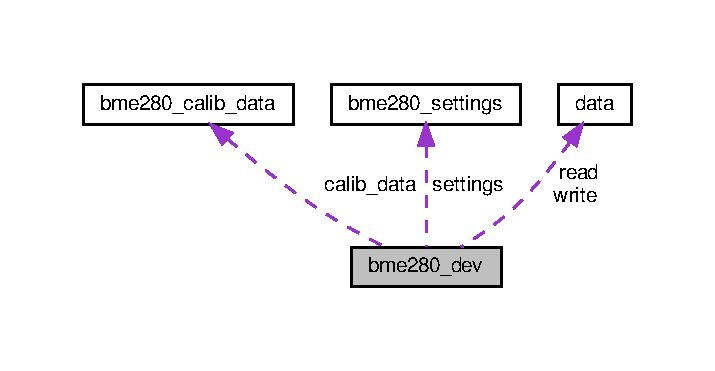
\includegraphics[width=343pt]{structbme280__dev__coll__graph}
\end{center}
\end{figure}
\subsection*{Public Attributes}
\begin{DoxyCompactItemize}
\item 
uint8\+\_\+t \hyperlink{structbme280__dev_a6147bb3590bc7d1b02c41454d13c81c0}{chip\+\_\+id}
\item 
uint8\+\_\+t \hyperlink{structbme280__dev_a1f75cc7ecf84476a440ded0cd8c2fba7}{dev\+\_\+id}
\item 
enum \hyperlink{group___b_m_e280_ga142fcd9cb1e99b793488e9b3b1e6766e}{bme280\+\_\+intf} \hyperlink{structbme280__dev_a937b25397d1455117b64b1380368d30c}{intf}
\item 
\hyperlink{group___b_m_e280_ga7c23fe68ccf92adb3f03882b40739e7b}{bme280\+\_\+com\+\_\+fptr\+\_\+t} \hyperlink{structbme280__dev_a9a0ad5b467e2acc04a854878fe71bf7f}{read}
\item 
\hyperlink{group___b_m_e280_ga7c23fe68ccf92adb3f03882b40739e7b}{bme280\+\_\+com\+\_\+fptr\+\_\+t} \hyperlink{structbme280__dev_a7d2437824573644b51b8514ca0ec294c}{write}
\item 
\hyperlink{group___b_m_e280_gab2783d9a00e56ddc3e0e8d37b3462e34}{bme280\+\_\+delay\+\_\+fptr\+\_\+t} \hyperlink{structbme280__dev_a8f8957a3f4438239bd79b075691f0fd1}{delay\+\_\+ms}
\item 
struct \hyperlink{structbme280__calib__data}{bme280\+\_\+calib\+\_\+data} \hyperlink{structbme280__dev_a8a57e57db020663dc3a8f3438cd6b399}{calib\+\_\+data}
\item 
struct \hyperlink{structbme280__settings}{bme280\+\_\+settings} \hyperlink{structbme280__dev_acd3efe8b8ac1e08f9cb21e8abec27042}{settings}
\end{DoxyCompactItemize}


\subsection{Detailed Description}
bme280 device structure 

\subsection{Member Data Documentation}
\mbox{\Hypertarget{structbme280__dev_a8a57e57db020663dc3a8f3438cd6b399}\label{structbme280__dev_a8a57e57db020663dc3a8f3438cd6b399}} 
\index{bme280\+\_\+dev@{bme280\+\_\+dev}!calib\+\_\+data@{calib\+\_\+data}}
\index{calib\+\_\+data@{calib\+\_\+data}!bme280\+\_\+dev@{bme280\+\_\+dev}}
\subsubsection{\texorpdfstring{calib\+\_\+data}{calib\_data}}
{\footnotesize\ttfamily struct \hyperlink{structbme280__calib__data}{bme280\+\_\+calib\+\_\+data} bme280\+\_\+dev\+::calib\+\_\+data}

Trim data \mbox{\Hypertarget{structbme280__dev_a6147bb3590bc7d1b02c41454d13c81c0}\label{structbme280__dev_a6147bb3590bc7d1b02c41454d13c81c0}} 
\index{bme280\+\_\+dev@{bme280\+\_\+dev}!chip\+\_\+id@{chip\+\_\+id}}
\index{chip\+\_\+id@{chip\+\_\+id}!bme280\+\_\+dev@{bme280\+\_\+dev}}
\subsubsection{\texorpdfstring{chip\+\_\+id}{chip\_id}}
{\footnotesize\ttfamily uint8\+\_\+t bme280\+\_\+dev\+::chip\+\_\+id}

Chip Id \mbox{\Hypertarget{structbme280__dev_a8f8957a3f4438239bd79b075691f0fd1}\label{structbme280__dev_a8f8957a3f4438239bd79b075691f0fd1}} 
\index{bme280\+\_\+dev@{bme280\+\_\+dev}!delay\+\_\+ms@{delay\+\_\+ms}}
\index{delay\+\_\+ms@{delay\+\_\+ms}!bme280\+\_\+dev@{bme280\+\_\+dev}}
\subsubsection{\texorpdfstring{delay\+\_\+ms}{delay\_ms}}
{\footnotesize\ttfamily \hyperlink{group___b_m_e280_gab2783d9a00e56ddc3e0e8d37b3462e34}{bme280\+\_\+delay\+\_\+fptr\+\_\+t} bme280\+\_\+dev\+::delay\+\_\+ms}

Delay function pointer \mbox{\Hypertarget{structbme280__dev_a1f75cc7ecf84476a440ded0cd8c2fba7}\label{structbme280__dev_a1f75cc7ecf84476a440ded0cd8c2fba7}} 
\index{bme280\+\_\+dev@{bme280\+\_\+dev}!dev\+\_\+id@{dev\+\_\+id}}
\index{dev\+\_\+id@{dev\+\_\+id}!bme280\+\_\+dev@{bme280\+\_\+dev}}
\subsubsection{\texorpdfstring{dev\+\_\+id}{dev\_id}}
{\footnotesize\ttfamily uint8\+\_\+t bme280\+\_\+dev\+::dev\+\_\+id}

Device Id \mbox{\Hypertarget{structbme280__dev_a937b25397d1455117b64b1380368d30c}\label{structbme280__dev_a937b25397d1455117b64b1380368d30c}} 
\index{bme280\+\_\+dev@{bme280\+\_\+dev}!intf@{intf}}
\index{intf@{intf}!bme280\+\_\+dev@{bme280\+\_\+dev}}
\subsubsection{\texorpdfstring{intf}{intf}}
{\footnotesize\ttfamily enum \hyperlink{group___b_m_e280_ga142fcd9cb1e99b793488e9b3b1e6766e}{bme280\+\_\+intf} bme280\+\_\+dev\+::intf}

S\+P\+I/\+I2C interface \mbox{\Hypertarget{structbme280__dev_a9a0ad5b467e2acc04a854878fe71bf7f}\label{structbme280__dev_a9a0ad5b467e2acc04a854878fe71bf7f}} 
\index{bme280\+\_\+dev@{bme280\+\_\+dev}!read@{read}}
\index{read@{read}!bme280\+\_\+dev@{bme280\+\_\+dev}}
\subsubsection{\texorpdfstring{read}{read}}
{\footnotesize\ttfamily \hyperlink{group___b_m_e280_ga7c23fe68ccf92adb3f03882b40739e7b}{bme280\+\_\+com\+\_\+fptr\+\_\+t} bme280\+\_\+dev\+::read}

Read function pointer \mbox{\Hypertarget{structbme280__dev_acd3efe8b8ac1e08f9cb21e8abec27042}\label{structbme280__dev_acd3efe8b8ac1e08f9cb21e8abec27042}} 
\index{bme280\+\_\+dev@{bme280\+\_\+dev}!settings@{settings}}
\index{settings@{settings}!bme280\+\_\+dev@{bme280\+\_\+dev}}
\subsubsection{\texorpdfstring{settings}{settings}}
{\footnotesize\ttfamily struct \hyperlink{structbme280__settings}{bme280\+\_\+settings} bme280\+\_\+dev\+::settings}

Sensor settings \mbox{\Hypertarget{structbme280__dev_a7d2437824573644b51b8514ca0ec294c}\label{structbme280__dev_a7d2437824573644b51b8514ca0ec294c}} 
\index{bme280\+\_\+dev@{bme280\+\_\+dev}!write@{write}}
\index{write@{write}!bme280\+\_\+dev@{bme280\+\_\+dev}}
\subsubsection{\texorpdfstring{write}{write}}
{\footnotesize\ttfamily \hyperlink{group___b_m_e280_ga7c23fe68ccf92adb3f03882b40739e7b}{bme280\+\_\+com\+\_\+fptr\+\_\+t} bme280\+\_\+dev\+::write}

Write function pointer 

The documentation for this struct was generated from the following file\+:\begin{DoxyCompactItemize}
\item 
sensor/\hyperlink{bme280__defs_8h}{bme280\+\_\+defs.\+h}\end{DoxyCompactItemize}

\hypertarget{structbme280__settings}{}\section{bme280\+\_\+settings Struct Reference}
\label{structbme280__settings}\index{bme280\+\_\+settings@{bme280\+\_\+settings}}


bme280 sensor settings structure which comprises of mode, oversampling and filter settings.  




{\ttfamily \#include $<$bme280\+\_\+defs.\+h$>$}

\subsection*{Public Attributes}
\begin{DoxyCompactItemize}
\item 
uint8\+\_\+t \hyperlink{structbme280__settings_a6359b35d9547f53dea01d893313c7dc3}{osr\+\_\+p}
\item 
uint8\+\_\+t \hyperlink{structbme280__settings_a49bf8f73813386b4dc37a9676230c263}{osr\+\_\+t}
\item 
uint8\+\_\+t \hyperlink{structbme280__settings_ab09e8c0b2ff1ee7e7eb35540ad95acf5}{osr\+\_\+h}
\item 
uint8\+\_\+t \hyperlink{structbme280__settings_a46eae004d968b4fd9a89e5cb5748f1c1}{filter}
\item 
uint8\+\_\+t \hyperlink{structbme280__settings_a9c881ed1a45bfd9092260383f13c9fbc}{standby\+\_\+time}
\end{DoxyCompactItemize}


\subsection{Detailed Description}
bme280 sensor settings structure which comprises of mode, oversampling and filter settings. 

\subsection{Member Data Documentation}
\mbox{\Hypertarget{structbme280__settings_a46eae004d968b4fd9a89e5cb5748f1c1}\label{structbme280__settings_a46eae004d968b4fd9a89e5cb5748f1c1}} 
\index{bme280\+\_\+settings@{bme280\+\_\+settings}!filter@{filter}}
\index{filter@{filter}!bme280\+\_\+settings@{bme280\+\_\+settings}}
\subsubsection{\texorpdfstring{filter}{filter}}
{\footnotesize\ttfamily uint8\+\_\+t bme280\+\_\+settings\+::filter}

filter coefficient \mbox{\Hypertarget{structbme280__settings_ab09e8c0b2ff1ee7e7eb35540ad95acf5}\label{structbme280__settings_ab09e8c0b2ff1ee7e7eb35540ad95acf5}} 
\index{bme280\+\_\+settings@{bme280\+\_\+settings}!osr\+\_\+h@{osr\+\_\+h}}
\index{osr\+\_\+h@{osr\+\_\+h}!bme280\+\_\+settings@{bme280\+\_\+settings}}
\subsubsection{\texorpdfstring{osr\+\_\+h}{osr\_h}}
{\footnotesize\ttfamily uint8\+\_\+t bme280\+\_\+settings\+::osr\+\_\+h}

humidity oversampling \mbox{\Hypertarget{structbme280__settings_a6359b35d9547f53dea01d893313c7dc3}\label{structbme280__settings_a6359b35d9547f53dea01d893313c7dc3}} 
\index{bme280\+\_\+settings@{bme280\+\_\+settings}!osr\+\_\+p@{osr\+\_\+p}}
\index{osr\+\_\+p@{osr\+\_\+p}!bme280\+\_\+settings@{bme280\+\_\+settings}}
\subsubsection{\texorpdfstring{osr\+\_\+p}{osr\_p}}
{\footnotesize\ttfamily uint8\+\_\+t bme280\+\_\+settings\+::osr\+\_\+p}

pressure oversampling \mbox{\Hypertarget{structbme280__settings_a49bf8f73813386b4dc37a9676230c263}\label{structbme280__settings_a49bf8f73813386b4dc37a9676230c263}} 
\index{bme280\+\_\+settings@{bme280\+\_\+settings}!osr\+\_\+t@{osr\+\_\+t}}
\index{osr\+\_\+t@{osr\+\_\+t}!bme280\+\_\+settings@{bme280\+\_\+settings}}
\subsubsection{\texorpdfstring{osr\+\_\+t}{osr\_t}}
{\footnotesize\ttfamily uint8\+\_\+t bme280\+\_\+settings\+::osr\+\_\+t}

temperature oversampling \mbox{\Hypertarget{structbme280__settings_a9c881ed1a45bfd9092260383f13c9fbc}\label{structbme280__settings_a9c881ed1a45bfd9092260383f13c9fbc}} 
\index{bme280\+\_\+settings@{bme280\+\_\+settings}!standby\+\_\+time@{standby\+\_\+time}}
\index{standby\+\_\+time@{standby\+\_\+time}!bme280\+\_\+settings@{bme280\+\_\+settings}}
\subsubsection{\texorpdfstring{standby\+\_\+time}{standby\_time}}
{\footnotesize\ttfamily uint8\+\_\+t bme280\+\_\+settings\+::standby\+\_\+time}

standby time 

The documentation for this struct was generated from the following file\+:\begin{DoxyCompactItemize}
\item 
sensor/\hyperlink{bme280__defs_8h}{bme280\+\_\+defs.\+h}\end{DoxyCompactItemize}

\hypertarget{structbme280__uncomp__data}{}\section{bme280\+\_\+uncomp\+\_\+data Struct Reference}
\label{structbme280__uncomp__data}\index{bme280\+\_\+uncomp\+\_\+data@{bme280\+\_\+uncomp\+\_\+data}}


bme280 sensor structure which comprises of uncompensated temperature, pressure and humidity data  




{\ttfamily \#include $<$bme280\+\_\+defs.\+h$>$}

\subsection*{Public Attributes}
\begin{DoxyCompactItemize}
\item 
uint32\+\_\+t \hyperlink{structbme280__uncomp__data_afa4d1b43f8412d393dcc5fd41f4203ce}{pressure}
\item 
uint32\+\_\+t \hyperlink{structbme280__uncomp__data_a0ae24e11ffef8390b948b53ba4dbb652}{temperature}
\item 
uint32\+\_\+t \hyperlink{structbme280__uncomp__data_a31e311e6fc9a49e8159a81017a7393a1}{humidity}
\end{DoxyCompactItemize}


\subsection{Detailed Description}
bme280 sensor structure which comprises of uncompensated temperature, pressure and humidity data 

\subsection{Member Data Documentation}
\mbox{\Hypertarget{structbme280__uncomp__data_a31e311e6fc9a49e8159a81017a7393a1}\label{structbme280__uncomp__data_a31e311e6fc9a49e8159a81017a7393a1}} 
\index{bme280\+\_\+uncomp\+\_\+data@{bme280\+\_\+uncomp\+\_\+data}!humidity@{humidity}}
\index{humidity@{humidity}!bme280\+\_\+uncomp\+\_\+data@{bme280\+\_\+uncomp\+\_\+data}}
\subsubsection{\texorpdfstring{humidity}{humidity}}
{\footnotesize\ttfamily uint32\+\_\+t bme280\+\_\+uncomp\+\_\+data\+::humidity}

un-\/compensated humidity \mbox{\Hypertarget{structbme280__uncomp__data_afa4d1b43f8412d393dcc5fd41f4203ce}\label{structbme280__uncomp__data_afa4d1b43f8412d393dcc5fd41f4203ce}} 
\index{bme280\+\_\+uncomp\+\_\+data@{bme280\+\_\+uncomp\+\_\+data}!pressure@{pressure}}
\index{pressure@{pressure}!bme280\+\_\+uncomp\+\_\+data@{bme280\+\_\+uncomp\+\_\+data}}
\subsubsection{\texorpdfstring{pressure}{pressure}}
{\footnotesize\ttfamily uint32\+\_\+t bme280\+\_\+uncomp\+\_\+data\+::pressure}

un-\/compensated pressure \mbox{\Hypertarget{structbme280__uncomp__data_a0ae24e11ffef8390b948b53ba4dbb652}\label{structbme280__uncomp__data_a0ae24e11ffef8390b948b53ba4dbb652}} 
\index{bme280\+\_\+uncomp\+\_\+data@{bme280\+\_\+uncomp\+\_\+data}!temperature@{temperature}}
\index{temperature@{temperature}!bme280\+\_\+uncomp\+\_\+data@{bme280\+\_\+uncomp\+\_\+data}}
\subsubsection{\texorpdfstring{temperature}{temperature}}
{\footnotesize\ttfamily uint32\+\_\+t bme280\+\_\+uncomp\+\_\+data\+::temperature}

un-\/compensated temperature 

The documentation for this struct was generated from the following file\+:\begin{DoxyCompactItemize}
\item 
sensor/\hyperlink{bme280__defs_8h}{bme280\+\_\+defs.\+h}\end{DoxyCompactItemize}

\hypertarget{structdata}{}\section{data Struct Reference}
\label{structdata}\index{data@{data}}


{\ttfamily \#include $<$sensor.\+h$>$}

\subsection*{Public Attributes}
\begin{DoxyCompactItemize}
\item 
int \hyperlink{structdata_ab041cff3ed545724b9157b87eaac1a08}{currenttime}
\item 
float \hyperlink{structdata_a92d573d048b933148a65e445b20df3b9}{temperature}
\item 
float \hyperlink{structdata_a6382da4e622ddd126cdc26169531e69f}{pressure}
\item 
float \hyperlink{structdata_a48291e0075fe9ab86708780888227e65}{humidity}
\end{DoxyCompactItemize}


\subsection{Member Data Documentation}
\mbox{\Hypertarget{structdata_ab041cff3ed545724b9157b87eaac1a08}\label{structdata_ab041cff3ed545724b9157b87eaac1a08}} 
\index{data@{data}!currenttime@{currenttime}}
\index{currenttime@{currenttime}!data@{data}}
\subsubsection{\texorpdfstring{currenttime}{currenttime}}
{\footnotesize\ttfamily int data\+::currenttime}

\mbox{\Hypertarget{structdata_a48291e0075fe9ab86708780888227e65}\label{structdata_a48291e0075fe9ab86708780888227e65}} 
\index{data@{data}!humidity@{humidity}}
\index{humidity@{humidity}!data@{data}}
\subsubsection{\texorpdfstring{humidity}{humidity}}
{\footnotesize\ttfamily float data\+::humidity}

\mbox{\Hypertarget{structdata_a6382da4e622ddd126cdc26169531e69f}\label{structdata_a6382da4e622ddd126cdc26169531e69f}} 
\index{data@{data}!pressure@{pressure}}
\index{pressure@{pressure}!data@{data}}
\subsubsection{\texorpdfstring{pressure}{pressure}}
{\footnotesize\ttfamily float data\+::pressure}

\mbox{\Hypertarget{structdata_a92d573d048b933148a65e445b20df3b9}\label{structdata_a92d573d048b933148a65e445b20df3b9}} 
\index{data@{data}!temperature@{temperature}}
\index{temperature@{temperature}!data@{data}}
\subsubsection{\texorpdfstring{temperature}{temperature}}
{\footnotesize\ttfamily float data\+::temperature}



The documentation for this struct was generated from the following file\+:\begin{DoxyCompactItemize}
\item 
sensor/\hyperlink{sensor_8h}{sensor.\+h}\end{DoxyCompactItemize}

\hypertarget{structdatatab}{}\section{datatab Struct Reference}
\label{structdatatab}\index{datatab@{datatab}}


{\ttfamily \#include $<$Metrics\+Average.\+h$>$}

\subsection*{Public Attributes}
\begin{DoxyCompactItemize}
\item 
int \hyperlink{structdatatab_ac19f083c0dcb6a011d92b76ca7f486e6}{currenttimetab} \mbox{[}10\mbox{]}
\item 
float \hyperlink{structdatatab_aff78d9a5fd529111ab738f41bb6120c5}{temperaturetab} \mbox{[}10\mbox{]}
\item 
float \hyperlink{structdatatab_ab8d11176f31a5fb8851108aa8547470c}{pressuretab} \mbox{[}10\mbox{]}
\item 
float \hyperlink{structdatatab_a60cf168a28c9c467fcc24674084de1b0}{humiditytab} \mbox{[}10\mbox{]}
\end{DoxyCompactItemize}


\subsection{Member Data Documentation}
\mbox{\Hypertarget{structdatatab_ac19f083c0dcb6a011d92b76ca7f486e6}\label{structdatatab_ac19f083c0dcb6a011d92b76ca7f486e6}} 
\index{datatab@{datatab}!currenttimetab@{currenttimetab}}
\index{currenttimetab@{currenttimetab}!datatab@{datatab}}
\subsubsection{\texorpdfstring{currenttimetab}{currenttimetab}}
{\footnotesize\ttfamily int datatab\+::currenttimetab\mbox{[}10\mbox{]}}

\mbox{\Hypertarget{structdatatab_a60cf168a28c9c467fcc24674084de1b0}\label{structdatatab_a60cf168a28c9c467fcc24674084de1b0}} 
\index{datatab@{datatab}!humiditytab@{humiditytab}}
\index{humiditytab@{humiditytab}!datatab@{datatab}}
\subsubsection{\texorpdfstring{humiditytab}{humiditytab}}
{\footnotesize\ttfamily float datatab\+::humiditytab\mbox{[}10\mbox{]}}

\mbox{\Hypertarget{structdatatab_ab8d11176f31a5fb8851108aa8547470c}\label{structdatatab_ab8d11176f31a5fb8851108aa8547470c}} 
\index{datatab@{datatab}!pressuretab@{pressuretab}}
\index{pressuretab@{pressuretab}!datatab@{datatab}}
\subsubsection{\texorpdfstring{pressuretab}{pressuretab}}
{\footnotesize\ttfamily float datatab\+::pressuretab\mbox{[}10\mbox{]}}

\mbox{\Hypertarget{structdatatab_aff78d9a5fd529111ab738f41bb6120c5}\label{structdatatab_aff78d9a5fd529111ab738f41bb6120c5}} 
\index{datatab@{datatab}!temperaturetab@{temperaturetab}}
\index{temperaturetab@{temperaturetab}!datatab@{datatab}}
\subsubsection{\texorpdfstring{temperaturetab}{temperaturetab}}
{\footnotesize\ttfamily float datatab\+::temperaturetab\mbox{[}10\mbox{]}}



The documentation for this struct was generated from the following file\+:\begin{DoxyCompactItemize}
\item 
sensor/\hyperlink{_metrics_average_8h}{Metrics\+Average.\+h}\end{DoxyCompactItemize}

\hypertarget{class_db_manager}{}\section{Db\+Manager Class Reference}
\label{class_db_manager}\index{Db\+Manager@{Db\+Manager}}


{\ttfamily \#include $<$dbmanager.\+h$>$}

\subsection*{Public Member Functions}
\begin{DoxyCompactItemize}
\item 
\hyperlink{class_db_manager_a0d16cf5bba931362e6c581eb1b5ba66a}{Db\+Manager} ()
\item 
\hyperlink{class_db_manager_a6427aaa42f5f4da4e86c52c2fd258729}{Db\+Manager} (const Q\+String path, const Q\+String name)
\item 
\hyperlink{class_db_manager_ac5cdf8e5e932d1681ab807d8f256374c}{$\sim$\+Db\+Manager} ()
\item 
bool \hyperlink{class_db_manager_ac04baba8f5d5197f8bcd9230393501de}{is\+Open} () const
\item 
bool \hyperlink{class_db_manager_a9dc0b40635f274bfda0470ac6b8fdf8e}{send\+Query} (Q\+String query) const
\item 
void \hyperlink{class_db_manager_ac31abceb0dd13bd030fc293f5f88797a}{send\+Query\+And\+Recieve} (Q\+String query)
\item 
bool \hyperlink{class_db_manager_a6730317c113a14f24fee2fe144feadcc}{create\+Db} (Q\+String path, Q\+String name)
\item 
bool \hyperlink{class_db_manager_a152a22868c32afd49431495b0ed97d28}{remove\+Db} (Q\+String path, Q\+String name)
\item 
bool \hyperlink{class_db_manager_ac8c34581c717a41e7585a6dabceec002}{create\+Table} ()
\item 
void \hyperlink{class_db_manager_a0d30e17db55d9a545b648b58d38409b6}{open\+Connection} (Q\+String path, Q\+String name)
\item 
void \hyperlink{class_db_manager_acbf62228942a303d4b914475803319f4}{close\+Connection} ()
\item 
bool \hyperlink{class_db_manager_ac428e3219240fa0432d9b2a037d1d00c}{add\+Metrics} (Q\+String temperature, Q\+String pressure, Q\+String humidity, Q\+String time)
\item 
bool \hyperlink{class_db_manager_a43a28838e80ae08ee2379a9d2f971e21}{add\+Zamb\+Forecast} (Q\+String forecast, Q\+String zambretti\+Num)
\item 
bool \hyperlink{class_db_manager_aec06961d5c5f828bddca53d57b1783c6}{add\+Metric} (Q\+String metric\+Value, Q\+String metric\+Name)
\item 
void \hyperlink{class_db_manager_a403b78f34127ab02882b55e345c39e8b}{print\+All\+Metrics} () const
\item 
bool \hyperlink{class_db_manager_a2a88468ac169883b9f77cfcf3ec853c9}{metric\+Exists} (Q\+String metric\+Name, const Q\+String \&value) const
\item 
bool \hyperlink{class_db_manager_a64af0d562c9800c63fd98392d0e00cd8}{remove\+All\+Metrics} ()
\item 
bool \hyperlink{class_db_manager_ad6ef7d9cc1952d1ae9ad263df5715e71}{remove\+Metric} (const Q\+String \&metric\+Name, Q\+String value)
\end{DoxyCompactItemize}


\subsection{Constructor \& Destructor Documentation}
\mbox{\Hypertarget{class_db_manager_a0d16cf5bba931362e6c581eb1b5ba66a}\label{class_db_manager_a0d16cf5bba931362e6c581eb1b5ba66a}} 
\index{Db\+Manager@{Db\+Manager}!Db\+Manager@{Db\+Manager}}
\index{Db\+Manager@{Db\+Manager}!Db\+Manager@{Db\+Manager}}
\subsubsection{\texorpdfstring{Db\+Manager()}{DbManager()}\hspace{0.1cm}{\footnotesize\ttfamily [1/2]}}
{\footnotesize\ttfamily Db\+Manager\+::\+Db\+Manager (\begin{DoxyParamCaption}{ }\end{DoxyParamCaption})}

\mbox{\Hypertarget{class_db_manager_a6427aaa42f5f4da4e86c52c2fd258729}\label{class_db_manager_a6427aaa42f5f4da4e86c52c2fd258729}} 
\index{Db\+Manager@{Db\+Manager}!Db\+Manager@{Db\+Manager}}
\index{Db\+Manager@{Db\+Manager}!Db\+Manager@{Db\+Manager}}
\subsubsection{\texorpdfstring{Db\+Manager()}{DbManager()}\hspace{0.1cm}{\footnotesize\ttfamily [2/2]}}
{\footnotesize\ttfamily Db\+Manager\+::\+Db\+Manager (\begin{DoxyParamCaption}\item[{const Q\+String}]{path,  }\item[{const Q\+String}]{name }\end{DoxyParamCaption})}

\mbox{\Hypertarget{class_db_manager_ac5cdf8e5e932d1681ab807d8f256374c}\label{class_db_manager_ac5cdf8e5e932d1681ab807d8f256374c}} 
\index{Db\+Manager@{Db\+Manager}!````~Db\+Manager@{$\sim$\+Db\+Manager}}
\index{````~Db\+Manager@{$\sim$\+Db\+Manager}!Db\+Manager@{Db\+Manager}}
\subsubsection{\texorpdfstring{$\sim$\+Db\+Manager()}{~DbManager()}}
{\footnotesize\ttfamily Db\+Manager\+::$\sim$\+Db\+Manager (\begin{DoxyParamCaption}{ }\end{DoxyParamCaption})}



\subsection{Member Function Documentation}
\mbox{\Hypertarget{class_db_manager_aec06961d5c5f828bddca53d57b1783c6}\label{class_db_manager_aec06961d5c5f828bddca53d57b1783c6}} 
\index{Db\+Manager@{Db\+Manager}!add\+Metric@{add\+Metric}}
\index{add\+Metric@{add\+Metric}!Db\+Manager@{Db\+Manager}}
\subsubsection{\texorpdfstring{add\+Metric()}{addMetric()}}
{\footnotesize\ttfamily bool Db\+Manager\+::add\+Metric (\begin{DoxyParamCaption}\item[{Q\+String}]{metric\+Value,  }\item[{Q\+String}]{metric\+Name }\end{DoxyParamCaption})}

\mbox{\Hypertarget{class_db_manager_ac428e3219240fa0432d9b2a037d1d00c}\label{class_db_manager_ac428e3219240fa0432d9b2a037d1d00c}} 
\index{Db\+Manager@{Db\+Manager}!add\+Metrics@{add\+Metrics}}
\index{add\+Metrics@{add\+Metrics}!Db\+Manager@{Db\+Manager}}
\subsubsection{\texorpdfstring{add\+Metrics()}{addMetrics()}}
{\footnotesize\ttfamily bool Db\+Manager\+::add\+Metrics (\begin{DoxyParamCaption}\item[{Q\+String}]{temperature,  }\item[{Q\+String}]{pressure,  }\item[{Q\+String}]{humidity,  }\item[{Q\+String}]{time }\end{DoxyParamCaption})}

\mbox{\Hypertarget{class_db_manager_a43a28838e80ae08ee2379a9d2f971e21}\label{class_db_manager_a43a28838e80ae08ee2379a9d2f971e21}} 
\index{Db\+Manager@{Db\+Manager}!add\+Zamb\+Forecast@{add\+Zamb\+Forecast}}
\index{add\+Zamb\+Forecast@{add\+Zamb\+Forecast}!Db\+Manager@{Db\+Manager}}
\subsubsection{\texorpdfstring{add\+Zamb\+Forecast()}{addZambForecast()}}
{\footnotesize\ttfamily bool Db\+Manager\+::add\+Zamb\+Forecast (\begin{DoxyParamCaption}\item[{Q\+String}]{forecast,  }\item[{Q\+String}]{zambretti\+Num }\end{DoxyParamCaption})}

\mbox{\Hypertarget{class_db_manager_acbf62228942a303d4b914475803319f4}\label{class_db_manager_acbf62228942a303d4b914475803319f4}} 
\index{Db\+Manager@{Db\+Manager}!close\+Connection@{close\+Connection}}
\index{close\+Connection@{close\+Connection}!Db\+Manager@{Db\+Manager}}
\subsubsection{\texorpdfstring{close\+Connection()}{closeConnection()}}
{\footnotesize\ttfamily void Db\+Manager\+::close\+Connection (\begin{DoxyParamCaption}{ }\end{DoxyParamCaption})}

\mbox{\Hypertarget{class_db_manager_a6730317c113a14f24fee2fe144feadcc}\label{class_db_manager_a6730317c113a14f24fee2fe144feadcc}} 
\index{Db\+Manager@{Db\+Manager}!create\+Db@{create\+Db}}
\index{create\+Db@{create\+Db}!Db\+Manager@{Db\+Manager}}
\subsubsection{\texorpdfstring{create\+Db()}{createDb()}}
{\footnotesize\ttfamily bool Db\+Manager\+::create\+Db (\begin{DoxyParamCaption}\item[{Q\+String}]{path,  }\item[{Q\+String}]{name }\end{DoxyParamCaption})}

\mbox{\Hypertarget{class_db_manager_ac8c34581c717a41e7585a6dabceec002}\label{class_db_manager_ac8c34581c717a41e7585a6dabceec002}} 
\index{Db\+Manager@{Db\+Manager}!create\+Table@{create\+Table}}
\index{create\+Table@{create\+Table}!Db\+Manager@{Db\+Manager}}
\subsubsection{\texorpdfstring{create\+Table()}{createTable()}}
{\footnotesize\ttfamily bool Db\+Manager\+::create\+Table (\begin{DoxyParamCaption}{ }\end{DoxyParamCaption})}

\mbox{\Hypertarget{class_db_manager_ac04baba8f5d5197f8bcd9230393501de}\label{class_db_manager_ac04baba8f5d5197f8bcd9230393501de}} 
\index{Db\+Manager@{Db\+Manager}!is\+Open@{is\+Open}}
\index{is\+Open@{is\+Open}!Db\+Manager@{Db\+Manager}}
\subsubsection{\texorpdfstring{is\+Open()}{isOpen()}}
{\footnotesize\ttfamily bool Db\+Manager\+::is\+Open (\begin{DoxyParamCaption}{ }\end{DoxyParamCaption}) const}

\mbox{\Hypertarget{class_db_manager_a2a88468ac169883b9f77cfcf3ec853c9}\label{class_db_manager_a2a88468ac169883b9f77cfcf3ec853c9}} 
\index{Db\+Manager@{Db\+Manager}!metric\+Exists@{metric\+Exists}}
\index{metric\+Exists@{metric\+Exists}!Db\+Manager@{Db\+Manager}}
\subsubsection{\texorpdfstring{metric\+Exists()}{metricExists()}}
{\footnotesize\ttfamily bool Db\+Manager\+::metric\+Exists (\begin{DoxyParamCaption}\item[{Q\+String}]{metric\+Name,  }\item[{const Q\+String \&}]{value }\end{DoxyParamCaption}) const}

\mbox{\Hypertarget{class_db_manager_a0d30e17db55d9a545b648b58d38409b6}\label{class_db_manager_a0d30e17db55d9a545b648b58d38409b6}} 
\index{Db\+Manager@{Db\+Manager}!open\+Connection@{open\+Connection}}
\index{open\+Connection@{open\+Connection}!Db\+Manager@{Db\+Manager}}
\subsubsection{\texorpdfstring{open\+Connection()}{openConnection()}}
{\footnotesize\ttfamily void Db\+Manager\+::open\+Connection (\begin{DoxyParamCaption}\item[{Q\+String}]{path,  }\item[{Q\+String}]{name }\end{DoxyParamCaption})}

\mbox{\Hypertarget{class_db_manager_a403b78f34127ab02882b55e345c39e8b}\label{class_db_manager_a403b78f34127ab02882b55e345c39e8b}} 
\index{Db\+Manager@{Db\+Manager}!print\+All\+Metrics@{print\+All\+Metrics}}
\index{print\+All\+Metrics@{print\+All\+Metrics}!Db\+Manager@{Db\+Manager}}
\subsubsection{\texorpdfstring{print\+All\+Metrics()}{printAllMetrics()}}
{\footnotesize\ttfamily void Db\+Manager\+::print\+All\+Metrics (\begin{DoxyParamCaption}{ }\end{DoxyParamCaption}) const}

\mbox{\Hypertarget{class_db_manager_a64af0d562c9800c63fd98392d0e00cd8}\label{class_db_manager_a64af0d562c9800c63fd98392d0e00cd8}} 
\index{Db\+Manager@{Db\+Manager}!remove\+All\+Metrics@{remove\+All\+Metrics}}
\index{remove\+All\+Metrics@{remove\+All\+Metrics}!Db\+Manager@{Db\+Manager}}
\subsubsection{\texorpdfstring{remove\+All\+Metrics()}{removeAllMetrics()}}
{\footnotesize\ttfamily bool Db\+Manager\+::remove\+All\+Metrics (\begin{DoxyParamCaption}{ }\end{DoxyParamCaption})}

\mbox{\Hypertarget{class_db_manager_a152a22868c32afd49431495b0ed97d28}\label{class_db_manager_a152a22868c32afd49431495b0ed97d28}} 
\index{Db\+Manager@{Db\+Manager}!remove\+Db@{remove\+Db}}
\index{remove\+Db@{remove\+Db}!Db\+Manager@{Db\+Manager}}
\subsubsection{\texorpdfstring{remove\+Db()}{removeDb()}}
{\footnotesize\ttfamily bool Db\+Manager\+::remove\+Db (\begin{DoxyParamCaption}\item[{Q\+String}]{path,  }\item[{Q\+String}]{name }\end{DoxyParamCaption})}

\mbox{\Hypertarget{class_db_manager_ad6ef7d9cc1952d1ae9ad263df5715e71}\label{class_db_manager_ad6ef7d9cc1952d1ae9ad263df5715e71}} 
\index{Db\+Manager@{Db\+Manager}!remove\+Metric@{remove\+Metric}}
\index{remove\+Metric@{remove\+Metric}!Db\+Manager@{Db\+Manager}}
\subsubsection{\texorpdfstring{remove\+Metric()}{removeMetric()}}
{\footnotesize\ttfamily bool Db\+Manager\+::remove\+Metric (\begin{DoxyParamCaption}\item[{const Q\+String \&}]{metric\+Name,  }\item[{Q\+String}]{value }\end{DoxyParamCaption})}

\mbox{\Hypertarget{class_db_manager_a9dc0b40635f274bfda0470ac6b8fdf8e}\label{class_db_manager_a9dc0b40635f274bfda0470ac6b8fdf8e}} 
\index{Db\+Manager@{Db\+Manager}!send\+Query@{send\+Query}}
\index{send\+Query@{send\+Query}!Db\+Manager@{Db\+Manager}}
\subsubsection{\texorpdfstring{send\+Query()}{sendQuery()}}
{\footnotesize\ttfamily bool Db\+Manager\+::send\+Query (\begin{DoxyParamCaption}\item[{Q\+String}]{query }\end{DoxyParamCaption}) const}

\mbox{\Hypertarget{class_db_manager_ac31abceb0dd13bd030fc293f5f88797a}\label{class_db_manager_ac31abceb0dd13bd030fc293f5f88797a}} 
\index{Db\+Manager@{Db\+Manager}!send\+Query\+And\+Recieve@{send\+Query\+And\+Recieve}}
\index{send\+Query\+And\+Recieve@{send\+Query\+And\+Recieve}!Db\+Manager@{Db\+Manager}}
\subsubsection{\texorpdfstring{send\+Query\+And\+Recieve()}{sendQueryAndRecieve()}}
{\footnotesize\ttfamily void Db\+Manager\+::send\+Query\+And\+Recieve (\begin{DoxyParamCaption}\item[{Q\+String}]{query }\end{DoxyParamCaption})}



The documentation for this class was generated from the following files\+:\begin{DoxyCompactItemize}
\item 
dbmanager/\hyperlink{dbmanager_8h}{dbmanager.\+h}\item 
dbmanager/\hyperlink{dbmanager_8cpp}{dbmanager.\+cpp}\end{DoxyCompactItemize}

\hypertarget{class_db_table}{}\section{Db\+Table Class Reference}
\label{class_db_table}\index{Db\+Table@{Db\+Table}}


{\ttfamily \#include $<$dbtable.\+h$>$}

\subsection*{Public Member Functions}
\begin{DoxyCompactItemize}
\item 
\hyperlink{class_db_table_a58c18caaf80638d74ca14f5599ae4248}{Db\+Table} (Q\+String temperature, Q\+String pressure, Q\+String humidity, Q\+String time)
\item 
\hyperlink{class_db_table_a3b61984342738abc45b6074e970eeb55}{$\sim$\+Db\+Table} ()
\item 
Q\+String \hyperlink{class_db_table_a7c3362a6fe703dc2c5fa3e217c52792f}{get\+Temperature} () const
\item 
Q\+String \hyperlink{class_db_table_afdc8c975dce8cfd9d578931252eb75cd}{get\+Pressure} () const
\item 
Q\+String \hyperlink{class_db_table_ad14c292fe435fe7b86f48554c75da206}{get\+Humidity} () const
\item 
Q\+String \hyperlink{class_db_table_aeffff61ff7c3a76e04bde211be25860f}{get\+Time} () const
\item 
void \hyperlink{class_db_table_acafd1019a86794179809e6a7b11d3c9f}{set\+Temperature} (const Q\+String \&value)
\item 
void \hyperlink{class_db_table_a14639cd693e8f6e1d48c0d263535a355}{set\+Pressure} (const Q\+String \&value)
\item 
void \hyperlink{class_db_table_a355eec4c57189589d85c5319b18a1b38}{set\+Humidity} (const Q\+String \&value)
\item 
void \hyperlink{class_db_table_a671e83deaebb40c81ada2bb7a92002b0}{set\+Time} (const Q\+String \&value)
\end{DoxyCompactItemize}


\subsection{Constructor \& Destructor Documentation}
\mbox{\Hypertarget{class_db_table_a58c18caaf80638d74ca14f5599ae4248}\label{class_db_table_a58c18caaf80638d74ca14f5599ae4248}} 
\index{Db\+Table@{Db\+Table}!Db\+Table@{Db\+Table}}
\index{Db\+Table@{Db\+Table}!Db\+Table@{Db\+Table}}
\subsubsection{\texorpdfstring{Db\+Table()}{DbTable()}}
{\footnotesize\ttfamily Db\+Table\+::\+Db\+Table (\begin{DoxyParamCaption}\item[{Q\+String}]{temperature,  }\item[{Q\+String}]{pressure,  }\item[{Q\+String}]{humidity,  }\item[{Q\+String}]{time }\end{DoxyParamCaption})}

\mbox{\Hypertarget{class_db_table_a3b61984342738abc45b6074e970eeb55}\label{class_db_table_a3b61984342738abc45b6074e970eeb55}} 
\index{Db\+Table@{Db\+Table}!````~Db\+Table@{$\sim$\+Db\+Table}}
\index{````~Db\+Table@{$\sim$\+Db\+Table}!Db\+Table@{Db\+Table}}
\subsubsection{\texorpdfstring{$\sim$\+Db\+Table()}{~DbTable()}}
{\footnotesize\ttfamily Db\+Table\+::$\sim$\+Db\+Table (\begin{DoxyParamCaption}{ }\end{DoxyParamCaption})}



\subsection{Member Function Documentation}
\mbox{\Hypertarget{class_db_table_ad14c292fe435fe7b86f48554c75da206}\label{class_db_table_ad14c292fe435fe7b86f48554c75da206}} 
\index{Db\+Table@{Db\+Table}!get\+Humidity@{get\+Humidity}}
\index{get\+Humidity@{get\+Humidity}!Db\+Table@{Db\+Table}}
\subsubsection{\texorpdfstring{get\+Humidity()}{getHumidity()}}
{\footnotesize\ttfamily Q\+String Db\+Table\+::get\+Humidity (\begin{DoxyParamCaption}{ }\end{DoxyParamCaption}) const}

\mbox{\Hypertarget{class_db_table_afdc8c975dce8cfd9d578931252eb75cd}\label{class_db_table_afdc8c975dce8cfd9d578931252eb75cd}} 
\index{Db\+Table@{Db\+Table}!get\+Pressure@{get\+Pressure}}
\index{get\+Pressure@{get\+Pressure}!Db\+Table@{Db\+Table}}
\subsubsection{\texorpdfstring{get\+Pressure()}{getPressure()}}
{\footnotesize\ttfamily Q\+String Db\+Table\+::get\+Pressure (\begin{DoxyParamCaption}{ }\end{DoxyParamCaption}) const}

\mbox{\Hypertarget{class_db_table_a7c3362a6fe703dc2c5fa3e217c52792f}\label{class_db_table_a7c3362a6fe703dc2c5fa3e217c52792f}} 
\index{Db\+Table@{Db\+Table}!get\+Temperature@{get\+Temperature}}
\index{get\+Temperature@{get\+Temperature}!Db\+Table@{Db\+Table}}
\subsubsection{\texorpdfstring{get\+Temperature()}{getTemperature()}}
{\footnotesize\ttfamily Q\+String Db\+Table\+::get\+Temperature (\begin{DoxyParamCaption}{ }\end{DoxyParamCaption}) const}

\mbox{\Hypertarget{class_db_table_aeffff61ff7c3a76e04bde211be25860f}\label{class_db_table_aeffff61ff7c3a76e04bde211be25860f}} 
\index{Db\+Table@{Db\+Table}!get\+Time@{get\+Time}}
\index{get\+Time@{get\+Time}!Db\+Table@{Db\+Table}}
\subsubsection{\texorpdfstring{get\+Time()}{getTime()}}
{\footnotesize\ttfamily Q\+String Db\+Table\+::get\+Time (\begin{DoxyParamCaption}{ }\end{DoxyParamCaption}) const}

\mbox{\Hypertarget{class_db_table_a355eec4c57189589d85c5319b18a1b38}\label{class_db_table_a355eec4c57189589d85c5319b18a1b38}} 
\index{Db\+Table@{Db\+Table}!set\+Humidity@{set\+Humidity}}
\index{set\+Humidity@{set\+Humidity}!Db\+Table@{Db\+Table}}
\subsubsection{\texorpdfstring{set\+Humidity()}{setHumidity()}}
{\footnotesize\ttfamily void Db\+Table\+::set\+Humidity (\begin{DoxyParamCaption}\item[{const Q\+String \&}]{value }\end{DoxyParamCaption})}

\mbox{\Hypertarget{class_db_table_a14639cd693e8f6e1d48c0d263535a355}\label{class_db_table_a14639cd693e8f6e1d48c0d263535a355}} 
\index{Db\+Table@{Db\+Table}!set\+Pressure@{set\+Pressure}}
\index{set\+Pressure@{set\+Pressure}!Db\+Table@{Db\+Table}}
\subsubsection{\texorpdfstring{set\+Pressure()}{setPressure()}}
{\footnotesize\ttfamily void Db\+Table\+::set\+Pressure (\begin{DoxyParamCaption}\item[{const Q\+String \&}]{value }\end{DoxyParamCaption})}

\mbox{\Hypertarget{class_db_table_acafd1019a86794179809e6a7b11d3c9f}\label{class_db_table_acafd1019a86794179809e6a7b11d3c9f}} 
\index{Db\+Table@{Db\+Table}!set\+Temperature@{set\+Temperature}}
\index{set\+Temperature@{set\+Temperature}!Db\+Table@{Db\+Table}}
\subsubsection{\texorpdfstring{set\+Temperature()}{setTemperature()}}
{\footnotesize\ttfamily void Db\+Table\+::set\+Temperature (\begin{DoxyParamCaption}\item[{const Q\+String \&}]{value }\end{DoxyParamCaption})}

\mbox{\Hypertarget{class_db_table_a671e83deaebb40c81ada2bb7a92002b0}\label{class_db_table_a671e83deaebb40c81ada2bb7a92002b0}} 
\index{Db\+Table@{Db\+Table}!set\+Time@{set\+Time}}
\index{set\+Time@{set\+Time}!Db\+Table@{Db\+Table}}
\subsubsection{\texorpdfstring{set\+Time()}{setTime()}}
{\footnotesize\ttfamily void Db\+Table\+::set\+Time (\begin{DoxyParamCaption}\item[{const Q\+String \&}]{value }\end{DoxyParamCaption})}



The documentation for this class was generated from the following files\+:\begin{DoxyCompactItemize}
\item 
dbmanager/\hyperlink{dbtable_8h}{dbtable.\+h}\item 
dbmanager/\hyperlink{dbtable_8cpp}{dbtable.\+cpp}\end{DoxyCompactItemize}

\hypertarget{class_metrics_average}{}\section{Metrics\+Average Class Reference}
\label{class_metrics_average}\index{Metrics\+Average@{Metrics\+Average}}


{\ttfamily \#include $<$Metrics\+Average.\+h$>$}

\subsection*{Public Member Functions}
\begin{DoxyCompactItemize}
\item 
\hyperlink{class_metrics_average_ae62764cf04f8b12618021c9c8dda927d}{Metrics\+Average} ()
\item 
\hyperlink{class_metrics_average_a6d76aae6b11e42433bb93c47568de695}{Metrics\+Average} (struct \hyperlink{structbme280__dev}{bme280\+\_\+dev} $\ast$dev)
\item 
void \hyperlink{class_metrics_average_ad7c1ebb802eb2b710fc823f82e4ecf7e}{measurevalue} ()
\item 
bool \hyperlink{class_metrics_average_a17fc55cc103b48439645e4cb48cd62d2}{get\+Sucess\+Initialization} ()
\item 
struct \hyperlink{structdata}{data} \hyperlink{class_metrics_average_aebeda8dfb7b624fe9cbbeb9b6dfc51e5}{get\+Data} ()
\item 
int \hyperlink{class_metrics_average_a225a5cef622b47b5388fec11c7c50df3}{rounded} (float x)
\item 
\hyperlink{class_metrics_average_a9c2595a58728d51bd2bb85ba3258966c}{$\sim$\+Metrics\+Average} ()
\item 
\hyperlink{structbme280__dev}{bme280\+\_\+dev} $\ast$ \hyperlink{class_metrics_average_ad476d4c4f04a3303d236dba4849c8045}{get\+Dev} () const
\item 
void \hyperlink{class_metrics_average_a73810dc84f599b5e2fc3b7b4c34f326c}{set\+Dev} (\hyperlink{structbme280__dev}{bme280\+\_\+dev} $\ast$dev)
\end{DoxyCompactItemize}


\subsection{Constructor \& Destructor Documentation}
\mbox{\Hypertarget{class_metrics_average_ae62764cf04f8b12618021c9c8dda927d}\label{class_metrics_average_ae62764cf04f8b12618021c9c8dda927d}} 
\index{Metrics\+Average@{Metrics\+Average}!Metrics\+Average@{Metrics\+Average}}
\index{Metrics\+Average@{Metrics\+Average}!Metrics\+Average@{Metrics\+Average}}
\subsubsection{\texorpdfstring{Metrics\+Average()}{MetricsAverage()}\hspace{0.1cm}{\footnotesize\ttfamily [1/2]}}
{\footnotesize\ttfamily Metrics\+Average\+::\+Metrics\+Average (\begin{DoxyParamCaption}{ }\end{DoxyParamCaption})}

\mbox{\Hypertarget{class_metrics_average_a6d76aae6b11e42433bb93c47568de695}\label{class_metrics_average_a6d76aae6b11e42433bb93c47568de695}} 
\index{Metrics\+Average@{Metrics\+Average}!Metrics\+Average@{Metrics\+Average}}
\index{Metrics\+Average@{Metrics\+Average}!Metrics\+Average@{Metrics\+Average}}
\subsubsection{\texorpdfstring{Metrics\+Average()}{MetricsAverage()}\hspace{0.1cm}{\footnotesize\ttfamily [2/2]}}
{\footnotesize\ttfamily Metrics\+Average\+::\+Metrics\+Average (\begin{DoxyParamCaption}\item[{struct \hyperlink{structbme280__dev}{bme280\+\_\+dev} $\ast$}]{dev }\end{DoxyParamCaption})}

\mbox{\Hypertarget{class_metrics_average_a9c2595a58728d51bd2bb85ba3258966c}\label{class_metrics_average_a9c2595a58728d51bd2bb85ba3258966c}} 
\index{Metrics\+Average@{Metrics\+Average}!````~Metrics\+Average@{$\sim$\+Metrics\+Average}}
\index{````~Metrics\+Average@{$\sim$\+Metrics\+Average}!Metrics\+Average@{Metrics\+Average}}
\subsubsection{\texorpdfstring{$\sim$\+Metrics\+Average()}{~MetricsAverage()}}
{\footnotesize\ttfamily Metrics\+Average\+::$\sim$\+Metrics\+Average (\begin{DoxyParamCaption}{ }\end{DoxyParamCaption})}



\subsection{Member Function Documentation}
\mbox{\Hypertarget{class_metrics_average_aebeda8dfb7b624fe9cbbeb9b6dfc51e5}\label{class_metrics_average_aebeda8dfb7b624fe9cbbeb9b6dfc51e5}} 
\index{Metrics\+Average@{Metrics\+Average}!get\+Data@{get\+Data}}
\index{get\+Data@{get\+Data}!Metrics\+Average@{Metrics\+Average}}
\subsubsection{\texorpdfstring{get\+Data()}{getData()}}
{\footnotesize\ttfamily struct \hyperlink{structdata}{data} Metrics\+Average\+::get\+Data (\begin{DoxyParamCaption}{ }\end{DoxyParamCaption})}

\mbox{\Hypertarget{class_metrics_average_ad476d4c4f04a3303d236dba4849c8045}\label{class_metrics_average_ad476d4c4f04a3303d236dba4849c8045}} 
\index{Metrics\+Average@{Metrics\+Average}!get\+Dev@{get\+Dev}}
\index{get\+Dev@{get\+Dev}!Metrics\+Average@{Metrics\+Average}}
\subsubsection{\texorpdfstring{get\+Dev()}{getDev()}}
{\footnotesize\ttfamily \hyperlink{structbme280__dev}{bme280\+\_\+dev} $\ast$ Metrics\+Average\+::get\+Dev (\begin{DoxyParamCaption}{ }\end{DoxyParamCaption}) const}

\mbox{\Hypertarget{class_metrics_average_a17fc55cc103b48439645e4cb48cd62d2}\label{class_metrics_average_a17fc55cc103b48439645e4cb48cd62d2}} 
\index{Metrics\+Average@{Metrics\+Average}!get\+Sucess\+Initialization@{get\+Sucess\+Initialization}}
\index{get\+Sucess\+Initialization@{get\+Sucess\+Initialization}!Metrics\+Average@{Metrics\+Average}}
\subsubsection{\texorpdfstring{get\+Sucess\+Initialization()}{getSucessInitialization()}}
{\footnotesize\ttfamily bool Metrics\+Average\+::get\+Sucess\+Initialization (\begin{DoxyParamCaption}{ }\end{DoxyParamCaption})}

\mbox{\Hypertarget{class_metrics_average_ad7c1ebb802eb2b710fc823f82e4ecf7e}\label{class_metrics_average_ad7c1ebb802eb2b710fc823f82e4ecf7e}} 
\index{Metrics\+Average@{Metrics\+Average}!measurevalue@{measurevalue}}
\index{measurevalue@{measurevalue}!Metrics\+Average@{Metrics\+Average}}
\subsubsection{\texorpdfstring{measurevalue()}{measurevalue()}}
{\footnotesize\ttfamily void Metrics\+Average\+::measurevalue (\begin{DoxyParamCaption}{ }\end{DoxyParamCaption})}

\mbox{\Hypertarget{class_metrics_average_a225a5cef622b47b5388fec11c7c50df3}\label{class_metrics_average_a225a5cef622b47b5388fec11c7c50df3}} 
\index{Metrics\+Average@{Metrics\+Average}!rounded@{rounded}}
\index{rounded@{rounded}!Metrics\+Average@{Metrics\+Average}}
\subsubsection{\texorpdfstring{rounded()}{rounded()}}
{\footnotesize\ttfamily int Metrics\+Average\+::rounded (\begin{DoxyParamCaption}\item[{float}]{x }\end{DoxyParamCaption})}

\mbox{\Hypertarget{class_metrics_average_a73810dc84f599b5e2fc3b7b4c34f326c}\label{class_metrics_average_a73810dc84f599b5e2fc3b7b4c34f326c}} 
\index{Metrics\+Average@{Metrics\+Average}!set\+Dev@{set\+Dev}}
\index{set\+Dev@{set\+Dev}!Metrics\+Average@{Metrics\+Average}}
\subsubsection{\texorpdfstring{set\+Dev()}{setDev()}}
{\footnotesize\ttfamily void Metrics\+Average\+::set\+Dev (\begin{DoxyParamCaption}\item[{\hyperlink{structbme280__dev}{bme280\+\_\+dev} $\ast$}]{dev }\end{DoxyParamCaption})}



The documentation for this class was generated from the following files\+:\begin{DoxyCompactItemize}
\item 
sensor/\hyperlink{_metrics_average_8h}{Metrics\+Average.\+h}\item 
sensor/\hyperlink{_metrics_average_8cpp}{Metrics\+Average.\+cpp}\end{DoxyCompactItemize}

\hypertarget{class_weather_data}{}\section{Weather\+Data Class Reference}
\label{class_weather_data}\index{Weather\+Data@{Weather\+Data}}


\mbox{[}0\mbox{]}  




{\ttfamily \#include $<$appmodel.\+h$>$}



Inheritance diagram for Weather\+Data\+:\nopagebreak
\begin{figure}[H]
\begin{center}
\leavevmode
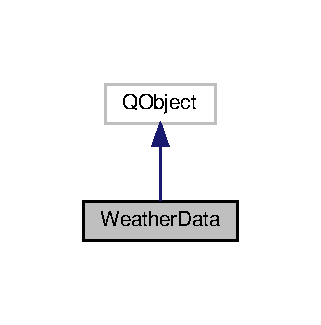
\includegraphics[width=154pt]{class_weather_data__inherit__graph}
\end{center}
\end{figure}
\subsection*{Signals}
\begin{DoxyCompactItemize}
\item 
void \hyperlink{class_weather_data_a23185106cf22ef8c57c96154e37b24d1}{data\+Changed} ()
\end{DoxyCompactItemize}
\subsection*{Public Member Functions}
\begin{DoxyCompactItemize}
\item 
\hyperlink{class_weather_data_aae42655299392d3f90feec9911a2dd60}{Weather\+Data} (Q\+Object $\ast$parent=0)
\item 
\hyperlink{class_weather_data_a48baeaa6b2a77d2a5e008159188416e8}{Weather\+Data} (const \hyperlink{class_weather_data}{Weather\+Data} \&other)
\item 
Q\+String \hyperlink{class_weather_data_a413b0ccf3fad036782ee5f5cb66f9a62}{day\+Of\+Week} () const
\item 
Q\+String \hyperlink{class_weather_data_a5baf2d9cc08741d7af4a07d61df95ee4}{weather\+Icon} () const
\item 
Q\+String \hyperlink{class_weather_data_a63a3528697c8681bd32d4d170ec91f76}{weather\+Description} () const
\item 
Q\+String \hyperlink{class_weather_data_a5a193e8410e3a146de59bab224cd88f0}{temperature} () const
\item 
Q\+String \hyperlink{class_weather_data_af726e713890bd6d310fe4a718dd69c77}{pressure} () const
\item 
Q\+String \hyperlink{class_weather_data_a0a83b2ee5398eaba062e3c6fe9264a3d}{humidity} () const
\item 
void \hyperlink{class_weather_data_ab47f3e7cde6cf4d93dfb1750ac014f00}{set\+Day\+Of\+Week} (const Q\+String \&value)
\item 
void \hyperlink{class_weather_data_a2a8093aaf20e1fb3c63c429a4ae0a977}{set\+Weather\+Icon} (const Q\+String \&value)
\item 
void \hyperlink{class_weather_data_a68686722f2e0bbf5cb28f0fdc96e280d}{set\+Weather\+Description} (const Q\+String \&value)
\item 
void \hyperlink{class_weather_data_afee514cbb8713059cf8d0602b33cadf5}{set\+Temperature} (const Q\+String \&value)
\item 
void \hyperlink{class_weather_data_ad5b453016656864e2bc3a09fc75919a0}{set\+Pressure} (const Q\+String \&\hyperlink{class_weather_data_af726e713890bd6d310fe4a718dd69c77}{pressure})
\item 
void \hyperlink{class_weather_data_aad895695b5f0651c58657973f2140509}{set\+Humidity} (const Q\+String \&\hyperlink{class_weather_data_a0a83b2ee5398eaba062e3c6fe9264a3d}{humidity})
\end{DoxyCompactItemize}
\subsection*{Properties}
\begin{DoxyCompactItemize}
\item 
Q\+String \hyperlink{class_weather_data_a483043396f44ae957716ebb005644d0d}{day\+Of\+Week}
\item 
Q\+String \hyperlink{class_weather_data_aca04e1877e2d5bc6da0f1e9910553741}{weather\+Icon}
\item 
Q\+String \hyperlink{class_weather_data_a8b470bc177e317a6a6a6b51758724a1a}{weather\+Description}
\item 
Q\+String \hyperlink{class_weather_data_a2ee510e51cb81a6a479cd0af5f291e2c}{temperature}
\end{DoxyCompactItemize}


\subsection{Detailed Description}
\mbox{[}0\mbox{]} 

\subsection{Constructor \& Destructor Documentation}
\mbox{\Hypertarget{class_weather_data_aae42655299392d3f90feec9911a2dd60}\label{class_weather_data_aae42655299392d3f90feec9911a2dd60}} 
\index{Weather\+Data@{Weather\+Data}!Weather\+Data@{Weather\+Data}}
\index{Weather\+Data@{Weather\+Data}!Weather\+Data@{Weather\+Data}}
\subsubsection{\texorpdfstring{Weather\+Data()}{WeatherData()}\hspace{0.1cm}{\footnotesize\ttfamily [1/2]}}
{\footnotesize\ttfamily Weather\+Data\+::\+Weather\+Data (\begin{DoxyParamCaption}\item[{Q\+Object $\ast$}]{parent = {\ttfamily 0} }\end{DoxyParamCaption})\hspace{0.3cm}{\ttfamily [explicit]}}

\mbox{\Hypertarget{class_weather_data_a48baeaa6b2a77d2a5e008159188416e8}\label{class_weather_data_a48baeaa6b2a77d2a5e008159188416e8}} 
\index{Weather\+Data@{Weather\+Data}!Weather\+Data@{Weather\+Data}}
\index{Weather\+Data@{Weather\+Data}!Weather\+Data@{Weather\+Data}}
\subsubsection{\texorpdfstring{Weather\+Data()}{WeatherData()}\hspace{0.1cm}{\footnotesize\ttfamily [2/2]}}
{\footnotesize\ttfamily Weather\+Data\+::\+Weather\+Data (\begin{DoxyParamCaption}\item[{const \hyperlink{class_weather_data}{Weather\+Data} \&}]{other }\end{DoxyParamCaption})}

Here is the call graph for this function\+:\nopagebreak
\begin{figure}[H]
\begin{center}
\leavevmode
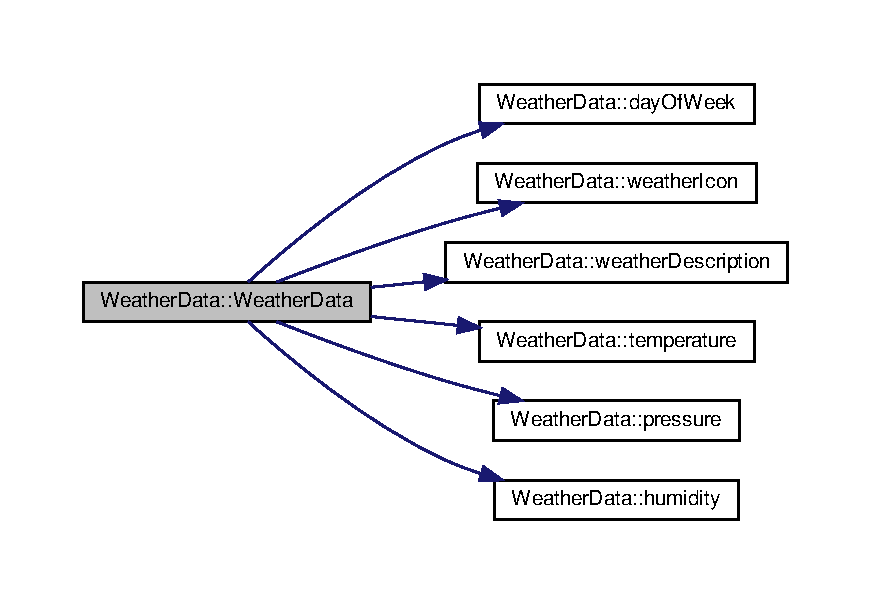
\includegraphics[width=350pt]{class_weather_data_a48baeaa6b2a77d2a5e008159188416e8_cgraph}
\end{center}
\end{figure}


\subsection{Member Function Documentation}
\mbox{\Hypertarget{class_weather_data_a23185106cf22ef8c57c96154e37b24d1}\label{class_weather_data_a23185106cf22ef8c57c96154e37b24d1}} 
\index{Weather\+Data@{Weather\+Data}!data\+Changed@{data\+Changed}}
\index{data\+Changed@{data\+Changed}!Weather\+Data@{Weather\+Data}}
\subsubsection{\texorpdfstring{data\+Changed}{dataChanged}}
{\footnotesize\ttfamily void Weather\+Data\+::data\+Changed (\begin{DoxyParamCaption}{ }\end{DoxyParamCaption})\hspace{0.3cm}{\ttfamily [signal]}}

Here is the caller graph for this function\+:\nopagebreak
\begin{figure}[H]
\begin{center}
\leavevmode
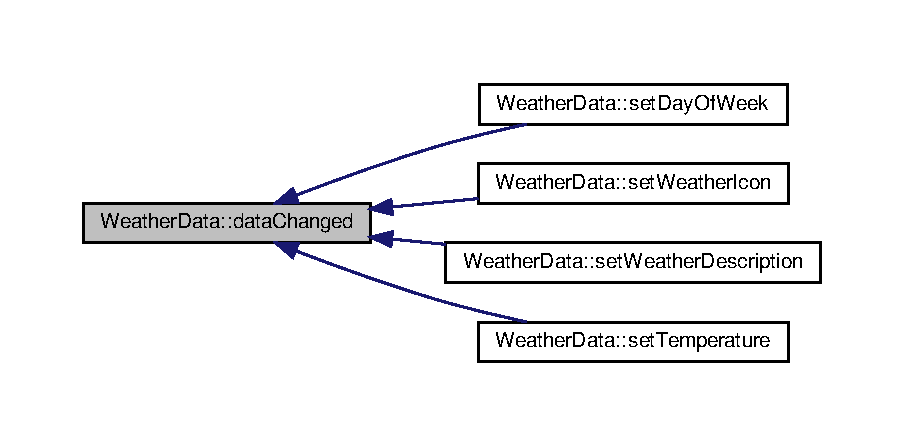
\includegraphics[width=350pt]{class_weather_data_a23185106cf22ef8c57c96154e37b24d1_icgraph}
\end{center}
\end{figure}
\mbox{\Hypertarget{class_weather_data_a413b0ccf3fad036782ee5f5cb66f9a62}\label{class_weather_data_a413b0ccf3fad036782ee5f5cb66f9a62}} 
\index{Weather\+Data@{Weather\+Data}!day\+Of\+Week@{day\+Of\+Week}}
\index{day\+Of\+Week@{day\+Of\+Week}!Weather\+Data@{Weather\+Data}}
\subsubsection{\texorpdfstring{day\+Of\+Week()}{dayOfWeek()}}
{\footnotesize\ttfamily Q\+String Weather\+Data\+::day\+Of\+Week (\begin{DoxyParamCaption}{ }\end{DoxyParamCaption}) const}

Here is the caller graph for this function\+:\nopagebreak
\begin{figure}[H]
\begin{center}
\leavevmode
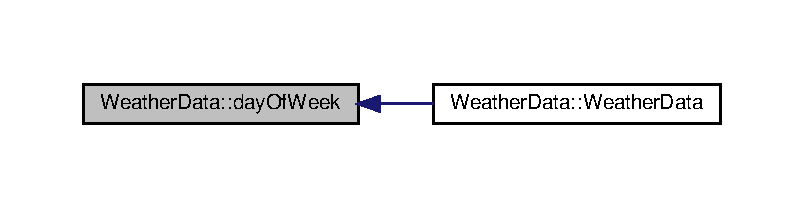
\includegraphics[width=350pt]{class_weather_data_a413b0ccf3fad036782ee5f5cb66f9a62_icgraph}
\end{center}
\end{figure}
\mbox{\Hypertarget{class_weather_data_a0a83b2ee5398eaba062e3c6fe9264a3d}\label{class_weather_data_a0a83b2ee5398eaba062e3c6fe9264a3d}} 
\index{Weather\+Data@{Weather\+Data}!humidity@{humidity}}
\index{humidity@{humidity}!Weather\+Data@{Weather\+Data}}
\subsubsection{\texorpdfstring{humidity()}{humidity()}}
{\footnotesize\ttfamily Q\+String Weather\+Data\+::humidity (\begin{DoxyParamCaption}{ }\end{DoxyParamCaption}) const}

Here is the caller graph for this function\+:\nopagebreak
\begin{figure}[H]
\begin{center}
\leavevmode
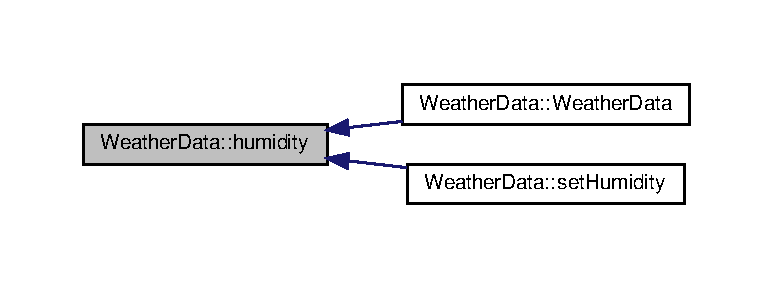
\includegraphics[width=350pt]{class_weather_data_a0a83b2ee5398eaba062e3c6fe9264a3d_icgraph}
\end{center}
\end{figure}
\mbox{\Hypertarget{class_weather_data_af726e713890bd6d310fe4a718dd69c77}\label{class_weather_data_af726e713890bd6d310fe4a718dd69c77}} 
\index{Weather\+Data@{Weather\+Data}!pressure@{pressure}}
\index{pressure@{pressure}!Weather\+Data@{Weather\+Data}}
\subsubsection{\texorpdfstring{pressure()}{pressure()}}
{\footnotesize\ttfamily Q\+String Weather\+Data\+::pressure (\begin{DoxyParamCaption}{ }\end{DoxyParamCaption}) const}

Here is the caller graph for this function\+:\nopagebreak
\begin{figure}[H]
\begin{center}
\leavevmode
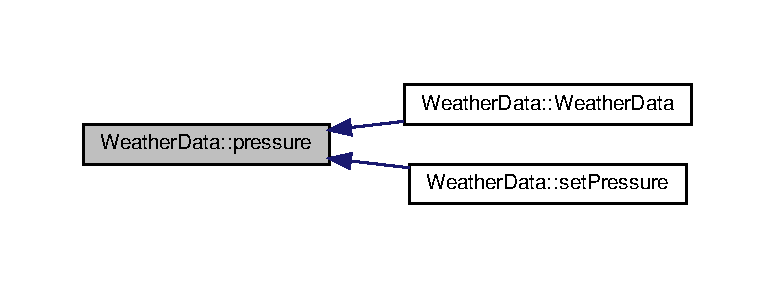
\includegraphics[width=350pt]{class_weather_data_af726e713890bd6d310fe4a718dd69c77_icgraph}
\end{center}
\end{figure}
\mbox{\Hypertarget{class_weather_data_ab47f3e7cde6cf4d93dfb1750ac014f00}\label{class_weather_data_ab47f3e7cde6cf4d93dfb1750ac014f00}} 
\index{Weather\+Data@{Weather\+Data}!set\+Day\+Of\+Week@{set\+Day\+Of\+Week}}
\index{set\+Day\+Of\+Week@{set\+Day\+Of\+Week}!Weather\+Data@{Weather\+Data}}
\subsubsection{\texorpdfstring{set\+Day\+Of\+Week()}{setDayOfWeek()}}
{\footnotesize\ttfamily void Weather\+Data\+::set\+Day\+Of\+Week (\begin{DoxyParamCaption}\item[{const Q\+String \&}]{value }\end{DoxyParamCaption})}

\mbox{\Hypertarget{class_weather_data_aad895695b5f0651c58657973f2140509}\label{class_weather_data_aad895695b5f0651c58657973f2140509}} 
\index{Weather\+Data@{Weather\+Data}!set\+Humidity@{set\+Humidity}}
\index{set\+Humidity@{set\+Humidity}!Weather\+Data@{Weather\+Data}}
\subsubsection{\texorpdfstring{set\+Humidity()}{setHumidity()}}
{\footnotesize\ttfamily void Weather\+Data\+::set\+Humidity (\begin{DoxyParamCaption}\item[{const Q\+String \&}]{humidity }\end{DoxyParamCaption})}

Here is the call graph for this function\+:\nopagebreak
\begin{figure}[H]
\begin{center}
\leavevmode
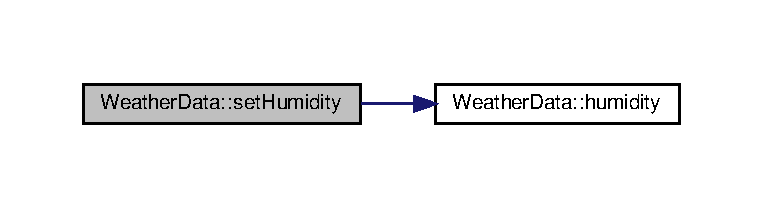
\includegraphics[width=350pt]{class_weather_data_aad895695b5f0651c58657973f2140509_cgraph}
\end{center}
\end{figure}
\mbox{\Hypertarget{class_weather_data_ad5b453016656864e2bc3a09fc75919a0}\label{class_weather_data_ad5b453016656864e2bc3a09fc75919a0}} 
\index{Weather\+Data@{Weather\+Data}!set\+Pressure@{set\+Pressure}}
\index{set\+Pressure@{set\+Pressure}!Weather\+Data@{Weather\+Data}}
\subsubsection{\texorpdfstring{set\+Pressure()}{setPressure()}}
{\footnotesize\ttfamily void Weather\+Data\+::set\+Pressure (\begin{DoxyParamCaption}\item[{const Q\+String \&}]{pressure }\end{DoxyParamCaption})}

Here is the call graph for this function\+:\nopagebreak
\begin{figure}[H]
\begin{center}
\leavevmode
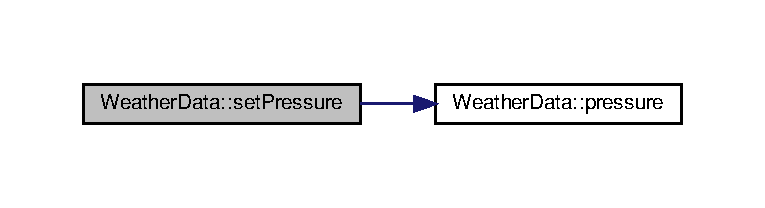
\includegraphics[width=350pt]{class_weather_data_ad5b453016656864e2bc3a09fc75919a0_cgraph}
\end{center}
\end{figure}
\mbox{\Hypertarget{class_weather_data_afee514cbb8713059cf8d0602b33cadf5}\label{class_weather_data_afee514cbb8713059cf8d0602b33cadf5}} 
\index{Weather\+Data@{Weather\+Data}!set\+Temperature@{set\+Temperature}}
\index{set\+Temperature@{set\+Temperature}!Weather\+Data@{Weather\+Data}}
\subsubsection{\texorpdfstring{set\+Temperature()}{setTemperature()}}
{\footnotesize\ttfamily void Weather\+Data\+::set\+Temperature (\begin{DoxyParamCaption}\item[{const Q\+String \&}]{value }\end{DoxyParamCaption})}

\mbox{\Hypertarget{class_weather_data_a68686722f2e0bbf5cb28f0fdc96e280d}\label{class_weather_data_a68686722f2e0bbf5cb28f0fdc96e280d}} 
\index{Weather\+Data@{Weather\+Data}!set\+Weather\+Description@{set\+Weather\+Description}}
\index{set\+Weather\+Description@{set\+Weather\+Description}!Weather\+Data@{Weather\+Data}}
\subsubsection{\texorpdfstring{set\+Weather\+Description()}{setWeatherDescription()}}
{\footnotesize\ttfamily void Weather\+Data\+::set\+Weather\+Description (\begin{DoxyParamCaption}\item[{const Q\+String \&}]{value }\end{DoxyParamCaption})}

\mbox{\Hypertarget{class_weather_data_a2a8093aaf20e1fb3c63c429a4ae0a977}\label{class_weather_data_a2a8093aaf20e1fb3c63c429a4ae0a977}} 
\index{Weather\+Data@{Weather\+Data}!set\+Weather\+Icon@{set\+Weather\+Icon}}
\index{set\+Weather\+Icon@{set\+Weather\+Icon}!Weather\+Data@{Weather\+Data}}
\subsubsection{\texorpdfstring{set\+Weather\+Icon()}{setWeatherIcon()}}
{\footnotesize\ttfamily void Weather\+Data\+::set\+Weather\+Icon (\begin{DoxyParamCaption}\item[{const Q\+String \&}]{value }\end{DoxyParamCaption})}

\mbox{\Hypertarget{class_weather_data_a5a193e8410e3a146de59bab224cd88f0}\label{class_weather_data_a5a193e8410e3a146de59bab224cd88f0}} 
\index{Weather\+Data@{Weather\+Data}!temperature@{temperature}}
\index{temperature@{temperature}!Weather\+Data@{Weather\+Data}}
\subsubsection{\texorpdfstring{temperature()}{temperature()}}
{\footnotesize\ttfamily Q\+String Weather\+Data\+::temperature (\begin{DoxyParamCaption}{ }\end{DoxyParamCaption}) const}

Here is the caller graph for this function\+:\nopagebreak
\begin{figure}[H]
\begin{center}
\leavevmode
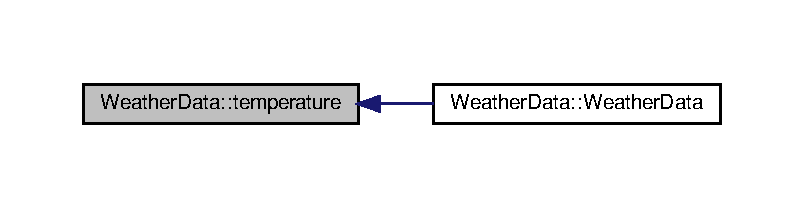
\includegraphics[width=350pt]{class_weather_data_a5a193e8410e3a146de59bab224cd88f0_icgraph}
\end{center}
\end{figure}
\mbox{\Hypertarget{class_weather_data_a63a3528697c8681bd32d4d170ec91f76}\label{class_weather_data_a63a3528697c8681bd32d4d170ec91f76}} 
\index{Weather\+Data@{Weather\+Data}!weather\+Description@{weather\+Description}}
\index{weather\+Description@{weather\+Description}!Weather\+Data@{Weather\+Data}}
\subsubsection{\texorpdfstring{weather\+Description()}{weatherDescription()}}
{\footnotesize\ttfamily Q\+String Weather\+Data\+::weather\+Description (\begin{DoxyParamCaption}{ }\end{DoxyParamCaption}) const}

Here is the caller graph for this function\+:\nopagebreak
\begin{figure}[H]
\begin{center}
\leavevmode
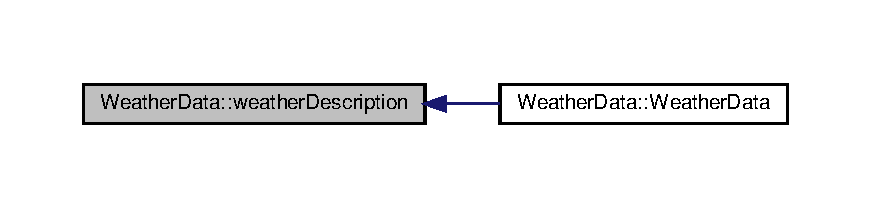
\includegraphics[width=350pt]{class_weather_data_a63a3528697c8681bd32d4d170ec91f76_icgraph}
\end{center}
\end{figure}
\mbox{\Hypertarget{class_weather_data_a5baf2d9cc08741d7af4a07d61df95ee4}\label{class_weather_data_a5baf2d9cc08741d7af4a07d61df95ee4}} 
\index{Weather\+Data@{Weather\+Data}!weather\+Icon@{weather\+Icon}}
\index{weather\+Icon@{weather\+Icon}!Weather\+Data@{Weather\+Data}}
\subsubsection{\texorpdfstring{weather\+Icon()}{weatherIcon()}}
{\footnotesize\ttfamily Q\+String Weather\+Data\+::weather\+Icon (\begin{DoxyParamCaption}{ }\end{DoxyParamCaption}) const}

Here is the caller graph for this function\+:\nopagebreak
\begin{figure}[H]
\begin{center}
\leavevmode
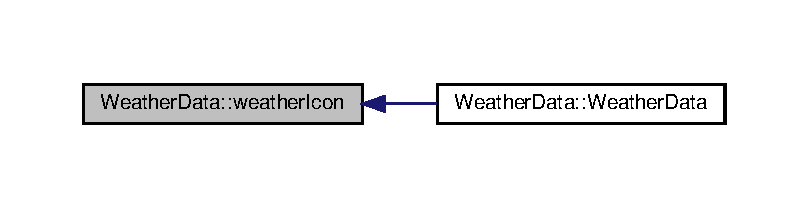
\includegraphics[width=350pt]{class_weather_data_a5baf2d9cc08741d7af4a07d61df95ee4_icgraph}
\end{center}
\end{figure}


\subsection{Property Documentation}
\mbox{\Hypertarget{class_weather_data_a483043396f44ae957716ebb005644d0d}\label{class_weather_data_a483043396f44ae957716ebb005644d0d}} 
\index{Weather\+Data@{Weather\+Data}!day\+Of\+Week@{day\+Of\+Week}}
\index{day\+Of\+Week@{day\+Of\+Week}!Weather\+Data@{Weather\+Data}}
\subsubsection{\texorpdfstring{day\+Of\+Week}{dayOfWeek}}
{\footnotesize\ttfamily Q\+String Weather\+Data\+::day\+Of\+Week\hspace{0.3cm}{\ttfamily [read]}, {\ttfamily [write]}}

\mbox{\Hypertarget{class_weather_data_a2ee510e51cb81a6a479cd0af5f291e2c}\label{class_weather_data_a2ee510e51cb81a6a479cd0af5f291e2c}} 
\index{Weather\+Data@{Weather\+Data}!temperature@{temperature}}
\index{temperature@{temperature}!Weather\+Data@{Weather\+Data}}
\subsubsection{\texorpdfstring{temperature}{temperature}}
{\footnotesize\ttfamily Q\+String Weather\+Data\+::temperature\hspace{0.3cm}{\ttfamily [read]}, {\ttfamily [write]}}

\mbox{\Hypertarget{class_weather_data_a8b470bc177e317a6a6a6b51758724a1a}\label{class_weather_data_a8b470bc177e317a6a6a6b51758724a1a}} 
\index{Weather\+Data@{Weather\+Data}!weather\+Description@{weather\+Description}}
\index{weather\+Description@{weather\+Description}!Weather\+Data@{Weather\+Data}}
\subsubsection{\texorpdfstring{weather\+Description}{weatherDescription}}
{\footnotesize\ttfamily Q\+String Weather\+Data\+::weather\+Description\hspace{0.3cm}{\ttfamily [read]}, {\ttfamily [write]}}

\mbox{\Hypertarget{class_weather_data_aca04e1877e2d5bc6da0f1e9910553741}\label{class_weather_data_aca04e1877e2d5bc6da0f1e9910553741}} 
\index{Weather\+Data@{Weather\+Data}!weather\+Icon@{weather\+Icon}}
\index{weather\+Icon@{weather\+Icon}!Weather\+Data@{Weather\+Data}}
\subsubsection{\texorpdfstring{weather\+Icon}{weatherIcon}}
{\footnotesize\ttfamily Q\+String Weather\+Data\+::weather\+Icon\hspace{0.3cm}{\ttfamily [read]}, {\ttfamily [write]}}

The icon value is based on Open\+Weather\+Map.\+org icon set. For details see \href{http://bugs.openweathermap.org/projects/api/wiki/Weather_Condition_Codes}{\tt http\+://bugs.\+openweathermap.\+org/projects/api/wiki/\+Weather\+\_\+\+Condition\+\_\+\+Codes}

e.\+g. 01d -\/$>$sunny day

The icon string will be translated to \href{http://openweathermap.org/img/w/01d.png}{\tt http\+://openweathermap.\+org/img/w/01d.\+png} 

The documentation for this class was generated from the following files\+:\begin{DoxyCompactItemize}
\item 
/home/jerome/projects/\+Weather\+Checking\+Rpi/weathercheckingrpi/\hyperlink{appmodel_8h}{appmodel.\+h}\item 
/home/jerome/projects/\+Weather\+Checking\+Rpi/weathercheckingrpi/\hyperlink{appmodel_8cpp}{appmodel.\+cpp}\end{DoxyCompactItemize}

\hypertarget{class_zambretti}{}\section{Zambretti Class Reference}
\label{class_zambretti}\index{Zambretti@{Zambretti}}


{\ttfamily \#include $<$Zambretti.\+h$>$}

\subsection*{Public Member Functions}
\begin{DoxyCompactItemize}
\item 
\hyperlink{class_zambretti_aa4948ec2096aefdbae2cebcdf8b80ee3}{Zambretti} ()
\item 
int \hyperlink{class_zambretti_ac46339c15cde0687b2008e4df0ecb4f9}{get\+Trend} ()
\item 
void \hyperlink{class_zambretti_a9237fb46dd347d7b0c5ecec1b9c4becc}{set\+Trend} (int currenttrend)
\item 
float \hyperlink{class_zambretti_ab7f8a79fbd772925a9e41c5789826385}{get\+Current\+Pressure} ()
\item 
int \hyperlink{class_zambretti_aac68758fdd41eb35c8ccd832e7b82e66}{get\+Znumber} ()
\item 
void \hyperlink{class_zambretti_a2722dff0af5aab457e344f9e4de0e6f2}{find\+Znumber} ()
\item 
\hyperlink{class_zambretti_a3066f3c5d93f8d08c34fc3a838e6b7f7}{$\sim$\+Zambretti} ()
\item 
void \hyperlink{class_zambretti_a9c0ea9c2f5d6b18f716b91c71088f208}{set\+Current\+Pressure} (float Current\+Pressure)
\item 
float \hyperlink{class_zambretti_a1c420aa581bae4f38859f110e6d2d876}{get\+Past\+Pressure} () const
\item 
void \hyperlink{class_zambretti_aaf38d93e2550c2c6f081f9d8f346e2fb}{set\+Past\+Pressure} (float Past\+Pressure)
\end{DoxyCompactItemize}


\subsection{Constructor \& Destructor Documentation}
\mbox{\Hypertarget{class_zambretti_aa4948ec2096aefdbae2cebcdf8b80ee3}\label{class_zambretti_aa4948ec2096aefdbae2cebcdf8b80ee3}} 
\index{Zambretti@{Zambretti}!Zambretti@{Zambretti}}
\index{Zambretti@{Zambretti}!Zambretti@{Zambretti}}
\subsubsection{\texorpdfstring{Zambretti()}{Zambretti()}}
{\footnotesize\ttfamily Zambretti\+::\+Zambretti (\begin{DoxyParamCaption}{ }\end{DoxyParamCaption})}

\mbox{\Hypertarget{class_zambretti_a3066f3c5d93f8d08c34fc3a838e6b7f7}\label{class_zambretti_a3066f3c5d93f8d08c34fc3a838e6b7f7}} 
\index{Zambretti@{Zambretti}!````~Zambretti@{$\sim$\+Zambretti}}
\index{````~Zambretti@{$\sim$\+Zambretti}!Zambretti@{Zambretti}}
\subsubsection{\texorpdfstring{$\sim$\+Zambretti()}{~Zambretti()}}
{\footnotesize\ttfamily Zambretti\+::$\sim$\+Zambretti (\begin{DoxyParamCaption}{ }\end{DoxyParamCaption})}



\subsection{Member Function Documentation}
\mbox{\Hypertarget{class_zambretti_a2722dff0af5aab457e344f9e4de0e6f2}\label{class_zambretti_a2722dff0af5aab457e344f9e4de0e6f2}} 
\index{Zambretti@{Zambretti}!find\+Znumber@{find\+Znumber}}
\index{find\+Znumber@{find\+Znumber}!Zambretti@{Zambretti}}
\subsubsection{\texorpdfstring{find\+Znumber()}{findZnumber()}}
{\footnotesize\ttfamily void Zambretti\+::find\+Znumber (\begin{DoxyParamCaption}{ }\end{DoxyParamCaption})}

\mbox{\Hypertarget{class_zambretti_ab7f8a79fbd772925a9e41c5789826385}\label{class_zambretti_ab7f8a79fbd772925a9e41c5789826385}} 
\index{Zambretti@{Zambretti}!get\+Current\+Pressure@{get\+Current\+Pressure}}
\index{get\+Current\+Pressure@{get\+Current\+Pressure}!Zambretti@{Zambretti}}
\subsubsection{\texorpdfstring{get\+Current\+Pressure()}{getCurrentPressure()}}
{\footnotesize\ttfamily float Zambretti\+::get\+Current\+Pressure (\begin{DoxyParamCaption}{ }\end{DoxyParamCaption})}

\mbox{\Hypertarget{class_zambretti_a1c420aa581bae4f38859f110e6d2d876}\label{class_zambretti_a1c420aa581bae4f38859f110e6d2d876}} 
\index{Zambretti@{Zambretti}!get\+Past\+Pressure@{get\+Past\+Pressure}}
\index{get\+Past\+Pressure@{get\+Past\+Pressure}!Zambretti@{Zambretti}}
\subsubsection{\texorpdfstring{get\+Past\+Pressure()}{getPastPressure()}}
{\footnotesize\ttfamily float Zambretti\+::get\+Past\+Pressure (\begin{DoxyParamCaption}{ }\end{DoxyParamCaption}) const}

\mbox{\Hypertarget{class_zambretti_ac46339c15cde0687b2008e4df0ecb4f9}\label{class_zambretti_ac46339c15cde0687b2008e4df0ecb4f9}} 
\index{Zambretti@{Zambretti}!get\+Trend@{get\+Trend}}
\index{get\+Trend@{get\+Trend}!Zambretti@{Zambretti}}
\subsubsection{\texorpdfstring{get\+Trend()}{getTrend()}}
{\footnotesize\ttfamily int Zambretti\+::get\+Trend (\begin{DoxyParamCaption}{ }\end{DoxyParamCaption})}

\mbox{\Hypertarget{class_zambretti_aac68758fdd41eb35c8ccd832e7b82e66}\label{class_zambretti_aac68758fdd41eb35c8ccd832e7b82e66}} 
\index{Zambretti@{Zambretti}!get\+Znumber@{get\+Znumber}}
\index{get\+Znumber@{get\+Znumber}!Zambretti@{Zambretti}}
\subsubsection{\texorpdfstring{get\+Znumber()}{getZnumber()}}
{\footnotesize\ttfamily int Zambretti\+::get\+Znumber (\begin{DoxyParamCaption}{ }\end{DoxyParamCaption})}

\mbox{\Hypertarget{class_zambretti_a9c0ea9c2f5d6b18f716b91c71088f208}\label{class_zambretti_a9c0ea9c2f5d6b18f716b91c71088f208}} 
\index{Zambretti@{Zambretti}!set\+Current\+Pressure@{set\+Current\+Pressure}}
\index{set\+Current\+Pressure@{set\+Current\+Pressure}!Zambretti@{Zambretti}}
\subsubsection{\texorpdfstring{set\+Current\+Pressure()}{setCurrentPressure()}}
{\footnotesize\ttfamily void Zambretti\+::set\+Current\+Pressure (\begin{DoxyParamCaption}\item[{float}]{Current\+Pressure }\end{DoxyParamCaption})}

\mbox{\Hypertarget{class_zambretti_aaf38d93e2550c2c6f081f9d8f346e2fb}\label{class_zambretti_aaf38d93e2550c2c6f081f9d8f346e2fb}} 
\index{Zambretti@{Zambretti}!set\+Past\+Pressure@{set\+Past\+Pressure}}
\index{set\+Past\+Pressure@{set\+Past\+Pressure}!Zambretti@{Zambretti}}
\subsubsection{\texorpdfstring{set\+Past\+Pressure()}{setPastPressure()}}
{\footnotesize\ttfamily void Zambretti\+::set\+Past\+Pressure (\begin{DoxyParamCaption}\item[{float}]{Past\+Pressure }\end{DoxyParamCaption})}

\mbox{\Hypertarget{class_zambretti_a9237fb46dd347d7b0c5ecec1b9c4becc}\label{class_zambretti_a9237fb46dd347d7b0c5ecec1b9c4becc}} 
\index{Zambretti@{Zambretti}!set\+Trend@{set\+Trend}}
\index{set\+Trend@{set\+Trend}!Zambretti@{Zambretti}}
\subsubsection{\texorpdfstring{set\+Trend()}{setTrend()}}
{\footnotesize\ttfamily void Zambretti\+::set\+Trend (\begin{DoxyParamCaption}\item[{int}]{currenttrend }\end{DoxyParamCaption})}



The documentation for this class was generated from the following files\+:\begin{DoxyCompactItemize}
\item 
zambretti/\hyperlink{_zambretti_8h}{Zambretti.\+h}\item 
zambretti/\hyperlink{_zambretti_8cpp}{Zambretti.\+cpp}\end{DoxyCompactItemize}

\chapter{File Documentation}
\hypertarget{appmodel_8cpp}{}\section{appmodel.\+cpp File Reference}
\label{appmodel_8cpp}\index{appmodel.\+cpp@{appmodel.\+cpp}}
{\ttfamily \#include \char`\"{}appmodel.\+h\char`\"{}}\newline
{\ttfamily \#include $<$Q\+Json\+Document$>$}\newline
{\ttfamily \#include $<$Q\+Json\+Object$>$}\newline
{\ttfamily \#include $<$Q\+Json\+Array$>$}\newline
{\ttfamily \#include $<$Q\+String\+List$>$}\newline
{\ttfamily \#include $<$Q\+Timer$>$}\newline
{\ttfamily \#include $<$Q\+File$>$}\newline
{\ttfamily \#include $<$Q\+Url\+Query$>$}\newline
{\ttfamily \#include $<$Q\+Elapsed\+Timer$>$}\newline
{\ttfamily \#include $<$Q\+Logging\+Category$>$}\newline
{\ttfamily \#include $<$Q\+Dir$>$}\newline
{\ttfamily \#include $<$Q\+Core\+Application$>$}\newline
{\ttfamily \#include \char`\"{}zambretti/\+Zambretti.\+h\char`\"{}}\newline
{\ttfamily \#include \char`\"{}sensor/\+Metrics\+Average.\+h\char`\"{}}\newline
{\ttfamily \#include \char`\"{}sensor/sensor.\+h\char`\"{}}\newline
{\ttfamily \#include $<$iostream$>$}\newline
Include dependency graph for appmodel.\+cpp\+:
\nopagebreak
\begin{figure}[H]
\begin{center}
\leavevmode
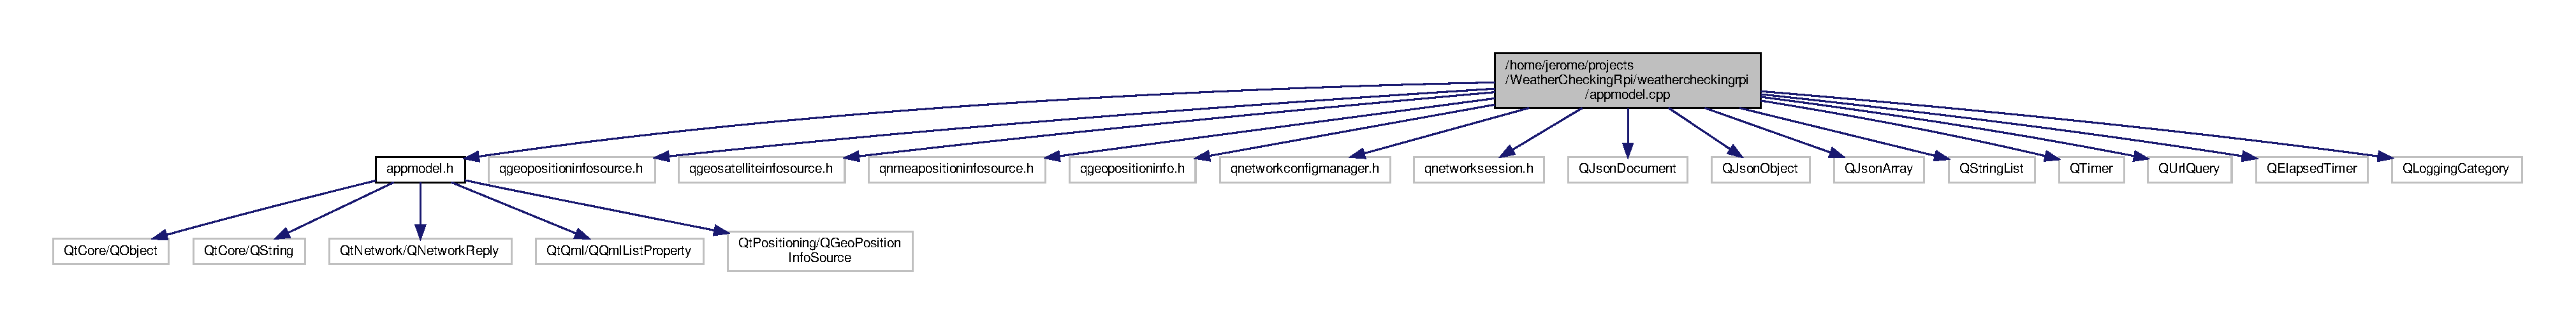
\includegraphics[width=350pt]{appmodel_8cpp__incl}
\end{center}
\end{figure}
\subsection*{Classes}
\begin{DoxyCompactItemize}
\item 
class \hyperlink{class_app_model_private}{App\+Model\+Private}
\end{DoxyCompactItemize}
\subsection*{Macros}
\begin{DoxyCompactItemize}
\item 
\#define \hyperlink{appmodel_8cpp_a6845ca0b7bf6295d883ba9ad80c2338c}{Z\+E\+R\+O\+\_\+\+K\+E\+L\+V\+IN}~273.\+15
\end{DoxyCompactItemize}


\subsection{Macro Definition Documentation}
\mbox{\Hypertarget{appmodel_8cpp_a6845ca0b7bf6295d883ba9ad80c2338c}\label{appmodel_8cpp_a6845ca0b7bf6295d883ba9ad80c2338c}} 
\index{appmodel.\+cpp@{appmodel.\+cpp}!Z\+E\+R\+O\+\_\+\+K\+E\+L\+V\+IN@{Z\+E\+R\+O\+\_\+\+K\+E\+L\+V\+IN}}
\index{Z\+E\+R\+O\+\_\+\+K\+E\+L\+V\+IN@{Z\+E\+R\+O\+\_\+\+K\+E\+L\+V\+IN}!appmodel.\+cpp@{appmodel.\+cpp}}
\subsubsection{\texorpdfstring{Z\+E\+R\+O\+\_\+\+K\+E\+L\+V\+IN}{ZERO\_KELVIN}}
{\footnotesize\ttfamily \#define Z\+E\+R\+O\+\_\+\+K\+E\+L\+V\+IN~273.\+15}


\hypertarget{appmodel_8h}{}\section{appmodel.\+h File Reference}
\label{appmodel_8h}\index{appmodel.\+h@{appmodel.\+h}}
{\ttfamily \#include $<$Qt\+Core/\+Q\+Object$>$}\newline
{\ttfamily \#include $<$Qt\+Core/\+Q\+String$>$}\newline
{\ttfamily \#include $<$Q\+Json\+Document$>$}\newline
{\ttfamily \#include \char`\"{}sensor/\+Metrics\+Average.\+h\char`\"{}}\newline
{\ttfamily \#include \char`\"{}sensor/sensor.\+h\char`\"{}}\newline
{\ttfamily \#include \char`\"{}zambretti/\+Zambretti.\+h\char`\"{}}\newline
Include dependency graph for appmodel.\+h\+:
\nopagebreak
\begin{figure}[H]
\begin{center}
\leavevmode
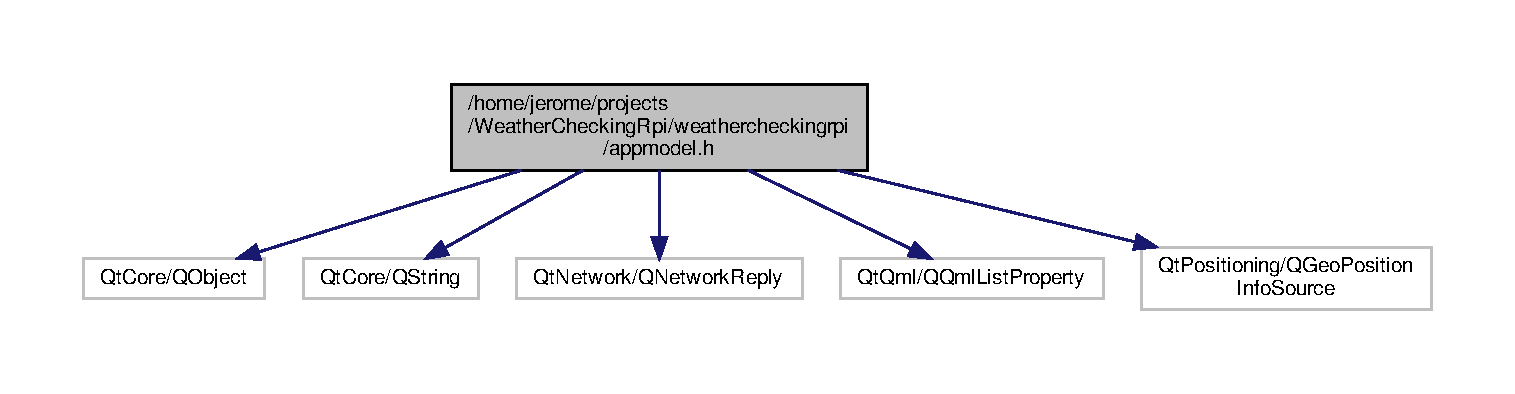
\includegraphics[width=350pt]{appmodel_8h__incl}
\end{center}
\end{figure}
This graph shows which files directly or indirectly include this file\+:
\nopagebreak
\begin{figure}[H]
\begin{center}
\leavevmode
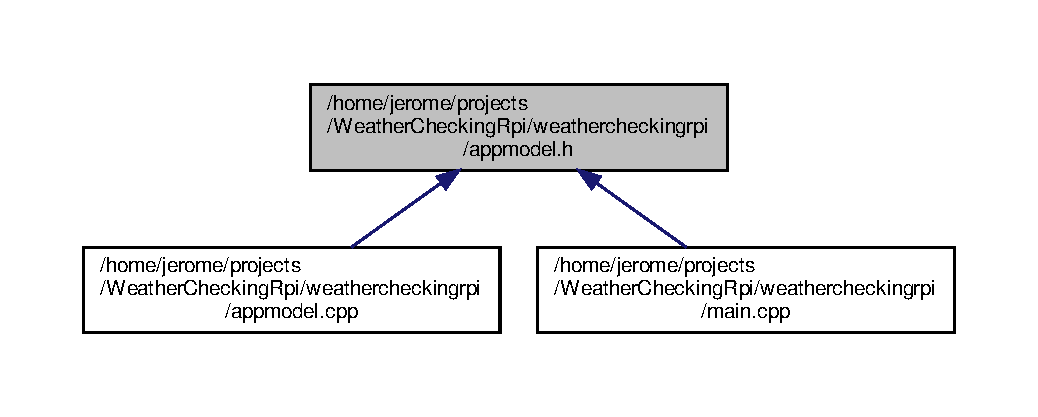
\includegraphics[width=232pt]{appmodel_8h__dep__incl}
\end{center}
\end{figure}
\subsection*{Classes}
\begin{DoxyCompactItemize}
\item 
class \hyperlink{class_weather_data}{Weather\+Data}
\item 
class \hyperlink{class_app_model}{App\+Model}
\end{DoxyCompactItemize}

\hypertarget{dbmanager_8cpp}{}\section{dbmanager/dbmanager.cpp File Reference}
\label{dbmanager_8cpp}\index{dbmanager/dbmanager.\+cpp@{dbmanager/dbmanager.\+cpp}}
{\ttfamily \#include \char`\"{}dbmanager.\+h\char`\"{}}\newline
{\ttfamily \#include $<$Q\+Debug$>$}\newline
{\ttfamily \#include $<$Qt\+Sql/\+Q\+Sql\+Query$>$}\newline
{\ttfamily \#include $<$Q\+Sql\+Error$>$}\newline
{\ttfamily \#include $<$Q\+Sql\+Record$>$}\newline
{\ttfamily \#include $<$Q\+File\+Info$>$}\newline
{\ttfamily \#include $<$Qt\+Gui/\+Q\+Gui\+Application$>$}\newline
{\ttfamily \#include $<$Qt\+Quick/\+Q\+Quick\+View$>$}\newline
{\ttfamily \#include $<$Qt\+Qml/\+Q\+Qml\+Engine$>$}\newline
{\ttfamily \#include $<$Qt\+Quick/\+Q\+Quick\+Item$>$}\newline
{\ttfamily \#include $<$map$>$}\newline
Include dependency graph for dbmanager.\+cpp\+:
\nopagebreak
\begin{figure}[H]
\begin{center}
\leavevmode
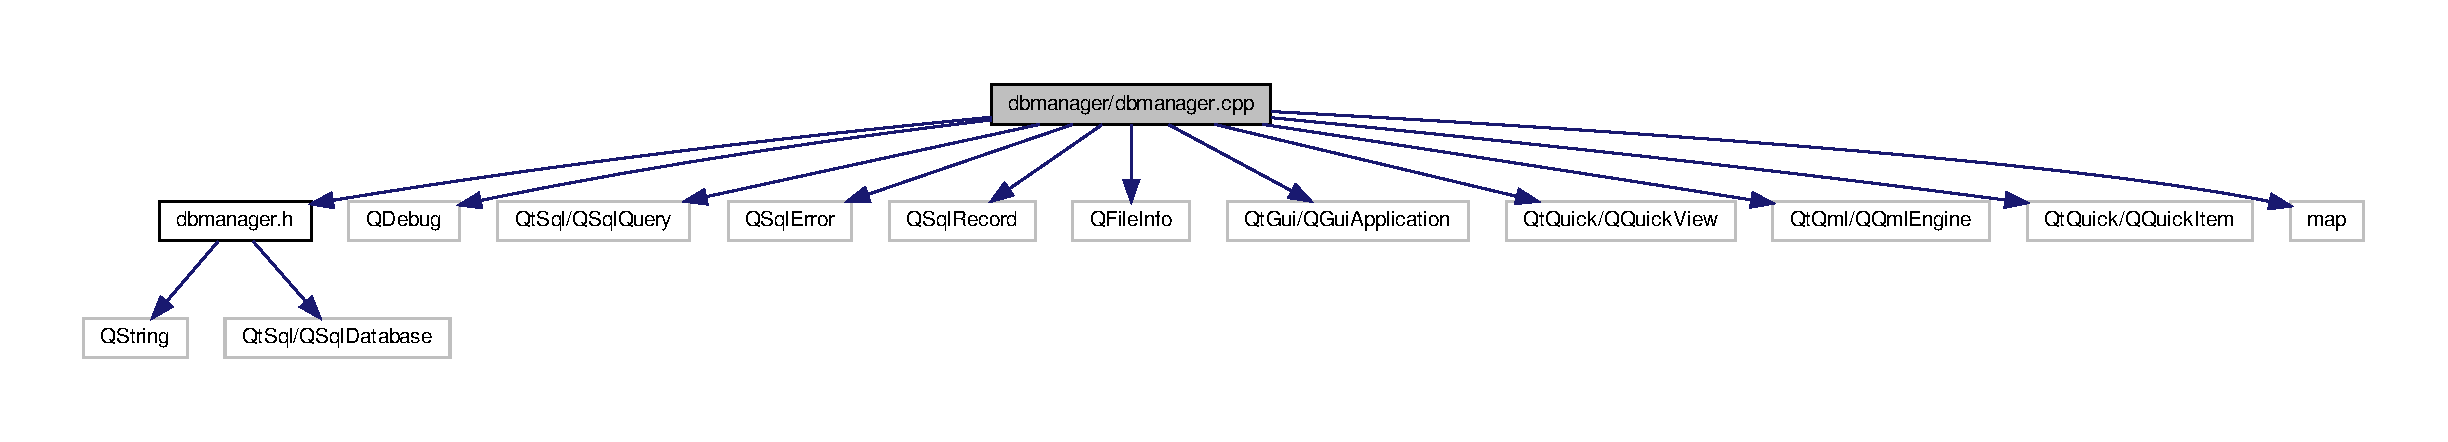
\includegraphics[width=350pt]{dbmanager_8cpp__incl}
\end{center}
\end{figure}

\hypertarget{dbmanager_8h}{}\section{dbmanager/dbmanager.h File Reference}
\label{dbmanager_8h}\index{dbmanager/dbmanager.\+h@{dbmanager/dbmanager.\+h}}
{\ttfamily \#include $<$Q\+String$>$}\newline
{\ttfamily \#include $<$Qt\+Sql/\+Q\+Sql\+Database$>$}\newline
Include dependency graph for dbmanager.\+h\+:
\nopagebreak
\begin{figure}[H]
\begin{center}
\leavevmode
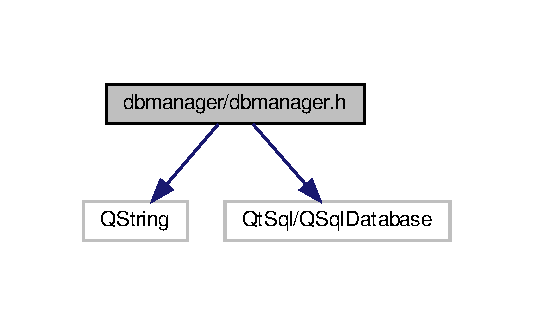
\includegraphics[width=256pt]{dbmanager_8h__incl}
\end{center}
\end{figure}
This graph shows which files directly or indirectly include this file\+:
\nopagebreak
\begin{figure}[H]
\begin{center}
\leavevmode
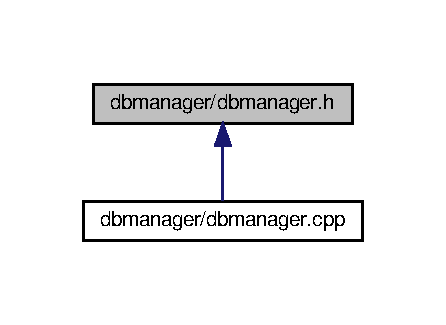
\includegraphics[width=214pt]{dbmanager_8h__dep__incl}
\end{center}
\end{figure}
\subsection*{Classes}
\begin{DoxyCompactItemize}
\item 
class \hyperlink{class_db_manager}{Db\+Manager}
\end{DoxyCompactItemize}

\hypertarget{dbtable_8cpp}{}\section{dbmanager/dbtable.cpp File Reference}
\label{dbtable_8cpp}\index{dbmanager/dbtable.\+cpp@{dbmanager/dbtable.\+cpp}}
{\ttfamily \#include \char`\"{}dbtable.\+h\char`\"{}}\newline
Include dependency graph for dbtable.\+cpp\+:
\nopagebreak
\begin{figure}[H]
\begin{center}
\leavevmode
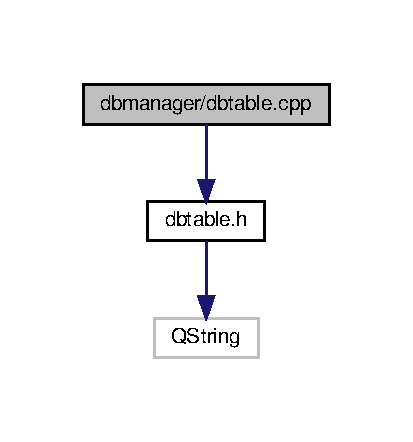
\includegraphics[width=198pt]{dbtable_8cpp__incl}
\end{center}
\end{figure}

\hypertarget{dbtable_8h}{}\section{dbmanager/dbtable.h File Reference}
\label{dbtable_8h}\index{dbmanager/dbtable.\+h@{dbmanager/dbtable.\+h}}
{\ttfamily \#include $<$Q\+String$>$}\newline
Include dependency graph for dbtable.\+h\+:
\nopagebreak
\begin{figure}[H]
\begin{center}
\leavevmode
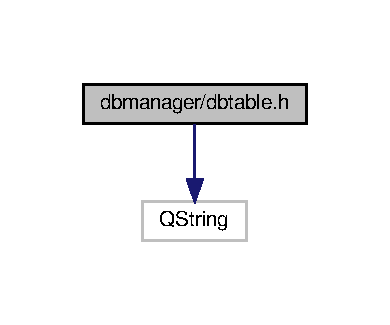
\includegraphics[width=187pt]{dbtable_8h__incl}
\end{center}
\end{figure}
This graph shows which files directly or indirectly include this file\+:
\nopagebreak
\begin{figure}[H]
\begin{center}
\leavevmode
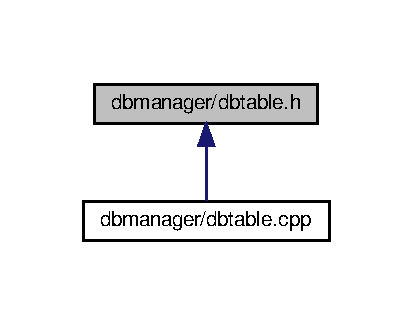
\includegraphics[width=198pt]{dbtable_8h__dep__incl}
\end{center}
\end{figure}
\subsection*{Classes}
\begin{DoxyCompactItemize}
\item 
class \hyperlink{class_db_table}{Db\+Table}
\end{DoxyCompactItemize}

\hypertarget{main_8cpp}{}\section{/home/jerome/projects/\+Weather\+Checking\+Rpi/weathercheckingrpi/main.cpp File Reference}
\label{main_8cpp}\index{/home/jerome/projects/\+Weather\+Checking\+Rpi/weathercheckingrpi/main.\+cpp@{/home/jerome/projects/\+Weather\+Checking\+Rpi/weathercheckingrpi/main.\+cpp}}
{\ttfamily \#include $<$Qt\+Gui/\+Q\+Gui\+Application$>$}\newline
{\ttfamily \#include $<$Qt\+Quick/\+Q\+Quick\+View$>$}\newline
{\ttfamily \#include $<$Qt\+Qml/\+Q\+Qml\+Engine$>$}\newline
{\ttfamily \#include $<$Qt\+Qml/\+Q\+Qml\+Context$>$}\newline
{\ttfamily \#include $<$Qt\+Quick/\+Q\+Quick\+Item$>$}\newline
{\ttfamily \#include $<$Q\+Logging\+Category$>$}\newline
{\ttfamily \#include \char`\"{}appmodel.\+h\char`\"{}}\newline
Include dependency graph for main.\+cpp\+:\nopagebreak
\begin{figure}[H]
\begin{center}
\leavevmode
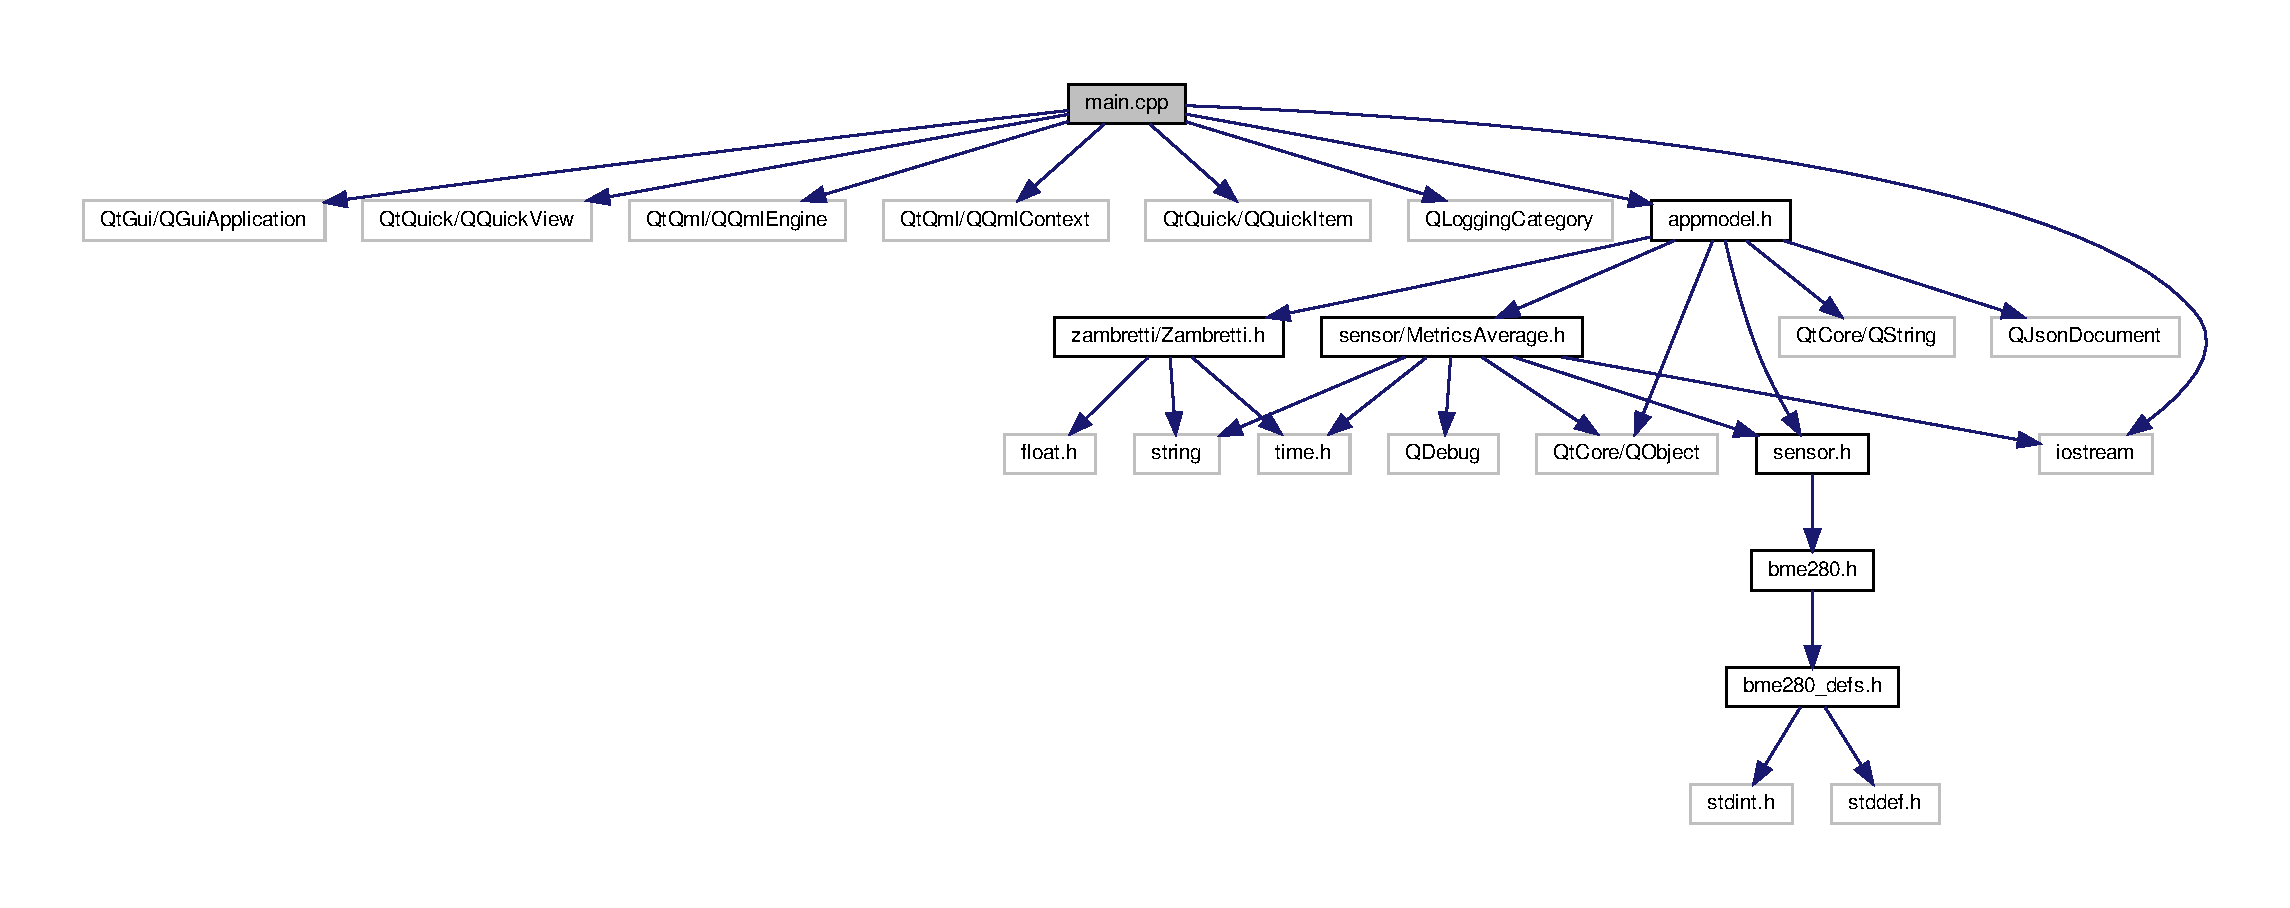
\includegraphics[width=350pt]{main_8cpp__incl}
\end{center}
\end{figure}
\subsection*{Functions}
\begin{DoxyCompactItemize}
\item 
int \hyperlink{main_8cpp_a0ddf1224851353fc92bfbff6f499fa97}{main} (int argc, char $\ast$argv\mbox{[}$\,$\mbox{]})
\begin{DoxyCompactList}\small\item\em \mbox{[}0\mbox{]} \end{DoxyCompactList}\end{DoxyCompactItemize}


\subsection{Function Documentation}
\mbox{\Hypertarget{main_8cpp_a0ddf1224851353fc92bfbff6f499fa97}\label{main_8cpp_a0ddf1224851353fc92bfbff6f499fa97}} 
\index{main.\+cpp@{main.\+cpp}!main@{main}}
\index{main@{main}!main.\+cpp@{main.\+cpp}}
\subsubsection{\texorpdfstring{main()}{main()}}
{\footnotesize\ttfamily int main (\begin{DoxyParamCaption}\item[{int}]{argc,  }\item[{char $\ast$}]{argv\mbox{[}$\,$\mbox{]} }\end{DoxyParamCaption})}



\mbox{[}0\mbox{]} 

\mbox{[}0\mbox{]}

\mbox{[}1\mbox{]} 
\hypertarget{zambretti_2main_8cpp}{}\section{zambretti/main.cpp File Reference}
\label{zambretti_2main_8cpp}\index{zambretti/main.\+cpp@{zambretti/main.\+cpp}}
{\ttfamily \#include \char`\"{}Zambretti.\+h\char`\"{}}\newline
{\ttfamily \#include $<$string$>$}\newline
{\ttfamily \#include $<$iostream$>$}\newline
{\ttfamily \#include $<$float.\+h$>$}\newline
Include dependency graph for main.\+cpp\+:
\nopagebreak
\begin{figure}[H]
\begin{center}
\leavevmode
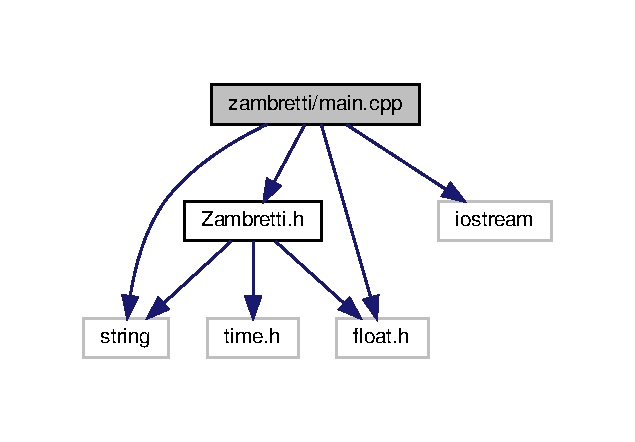
\includegraphics[width=305pt]{zambretti_2main_8cpp__incl}
\end{center}
\end{figure}
\subsection*{Functions}
\begin{DoxyCompactItemize}
\item 
int \hyperlink{zambretti_2main_8cpp_a840291bc02cba5474a4cb46a9b9566fe}{main} (void)
\end{DoxyCompactItemize}


\subsection{Function Documentation}
\mbox{\Hypertarget{zambretti_2main_8cpp_a840291bc02cba5474a4cb46a9b9566fe}\label{zambretti_2main_8cpp_a840291bc02cba5474a4cb46a9b9566fe}} 
\index{zambretti/main.\+cpp@{zambretti/main.\+cpp}!main@{main}}
\index{main@{main}!zambretti/main.\+cpp@{zambretti/main.\+cpp}}
\subsubsection{\texorpdfstring{main()}{main()}}
{\footnotesize\ttfamily int main (\begin{DoxyParamCaption}\item[{void}]{ }\end{DoxyParamCaption})}


\hypertarget{bme280_8c}{}\section{sensor/bme280.c File Reference}
\label{bme280_8c}\index{sensor/bme280.\+c@{sensor/bme280.\+c}}


Sensor driver for B\+M\+E280 sensor.  


{\ttfamily \#include \char`\"{}bme280.\+h\char`\"{}}\newline
Include dependency graph for bme280.\+c\+:
\nopagebreak
\begin{figure}[H]
\begin{center}
\leavevmode
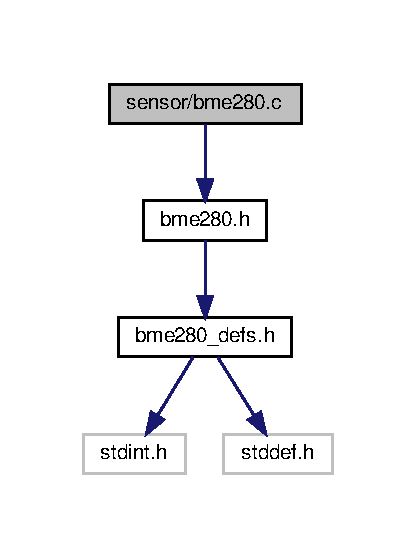
\includegraphics[width=200pt]{bme280_8c__incl}
\end{center}
\end{figure}
\subsection*{Internal macros}
\begin{DoxyCompactItemize}
\item 
\#define \hyperlink{bme280_8c_a17c5a85c1a9613150ab6a7f798baa427}{O\+V\+E\+R\+S\+A\+M\+P\+L\+I\+N\+G\+\_\+\+S\+E\+T\+T\+I\+N\+GS}~\hyperlink{group___b_m_e280_gacd2aa09844a8a245cf7fdbb808e215e5}{U\+I\+N\+T8\+\_\+C}(0x07)
\item 
\#define \hyperlink{bme280_8c_a124daa6c7034cbf83e4380265fc5c3f6}{F\+I\+L\+T\+E\+R\+\_\+\+S\+T\+A\+N\+D\+B\+Y\+\_\+\+S\+E\+T\+T\+I\+N\+GS}~\hyperlink{group___b_m_e280_gacd2aa09844a8a245cf7fdbb808e215e5}{U\+I\+N\+T8\+\_\+C}(0x18)
\item 
int8\+\_\+t \hyperlink{group___b_m_e280_gaf0b7d7a19bb48ec9eb3651b79f0c3e85}{bme280\+\_\+init} (struct \hyperlink{structbme280__dev}{bme280\+\_\+dev} $\ast$dev)
\begin{DoxyCompactList}\small\item\em This A\+PI is the entry point. It reads the chip-\/id and calibration data from the sensor. \end{DoxyCompactList}\item 
int8\+\_\+t \hyperlink{group___b_m_e280_ga992c5a438b414fe4724764738b88d9d7}{bme280\+\_\+get\+\_\+regs} (uint8\+\_\+t reg\+\_\+addr, uint8\+\_\+t $\ast$reg\+\_\+data, uint16\+\_\+t len, const struct \hyperlink{structbme280__dev}{bme280\+\_\+dev} $\ast$dev)
\begin{DoxyCompactList}\small\item\em This A\+PI reads the data from the given register address of the sensor. \end{DoxyCompactList}\item 
int8\+\_\+t \hyperlink{group___b_m_e280_ga002175df0ebe7893fcf0a54dfe806ba1}{bme280\+\_\+set\+\_\+regs} (uint8\+\_\+t $\ast$reg\+\_\+addr, const uint8\+\_\+t $\ast$reg\+\_\+data, uint8\+\_\+t len, const struct \hyperlink{structbme280__dev}{bme280\+\_\+dev} $\ast$dev)
\begin{DoxyCompactList}\small\item\em This A\+PI writes the given data to the register address of the sensor. \end{DoxyCompactList}\item 
int8\+\_\+t \hyperlink{group___b_m_e280_ga5d436d907394fde22471347599948205}{bme280\+\_\+set\+\_\+sensor\+\_\+settings} (uint8\+\_\+t desired\+\_\+settings, const struct \hyperlink{structbme280__dev}{bme280\+\_\+dev} $\ast$dev)
\begin{DoxyCompactList}\small\item\em This A\+PI sets the oversampling, filter and standby duration (normal mode) settings in the sensor. \end{DoxyCompactList}\item 
int8\+\_\+t \hyperlink{group___b_m_e280_gaf3bef90d33942197a98715ea8657211f}{bme280\+\_\+get\+\_\+sensor\+\_\+settings} (struct \hyperlink{structbme280__dev}{bme280\+\_\+dev} $\ast$dev)
\begin{DoxyCompactList}\small\item\em This A\+PI gets the oversampling, filter and standby duration (normal mode) settings from the sensor. \end{DoxyCompactList}\item 
int8\+\_\+t \hyperlink{group___b_m_e280_ga17a0eaeb97e43233af3e6aac8bd426d4}{bme280\+\_\+set\+\_\+sensor\+\_\+mode} (uint8\+\_\+t sensor\+\_\+mode, const struct \hyperlink{structbme280__dev}{bme280\+\_\+dev} $\ast$dev)
\begin{DoxyCompactList}\small\item\em This A\+PI sets the power mode of the sensor. \end{DoxyCompactList}\item 
int8\+\_\+t \hyperlink{group___b_m_e280_ga4e9e8d290d842abb3262591ff9f64bc4}{bme280\+\_\+get\+\_\+sensor\+\_\+mode} (uint8\+\_\+t $\ast$sensor\+\_\+mode, const struct \hyperlink{structbme280__dev}{bme280\+\_\+dev} $\ast$dev)
\begin{DoxyCompactList}\small\item\em This A\+PI gets the power mode of the sensor. \end{DoxyCompactList}\item 
int8\+\_\+t \hyperlink{group___b_m_e280_ga90dd2358e7050455585842a0fd468f97}{bme280\+\_\+soft\+\_\+reset} (const struct \hyperlink{structbme280__dev}{bme280\+\_\+dev} $\ast$dev)
\begin{DoxyCompactList}\small\item\em This A\+PI performs the soft reset of the sensor. \end{DoxyCompactList}\item 
int8\+\_\+t \hyperlink{group___b_m_e280_ga6671fea2c1e01f40029a653b9ab4410d}{bme280\+\_\+get\+\_\+sensor\+\_\+data} (uint8\+\_\+t sensor\+\_\+comp, struct \hyperlink{structbme280__data}{bme280\+\_\+data} $\ast$comp\+\_\+data, struct \hyperlink{structbme280__dev}{bme280\+\_\+dev} $\ast$dev)
\begin{DoxyCompactList}\small\item\em This A\+PI reads the pressure, temperature and humidity data from the sensor, compensates the data and store it in the \hyperlink{structbme280__data}{bme280\+\_\+data} structure instance passed by the user. \end{DoxyCompactList}\item 
void \hyperlink{group___b_m_e280_ga84be45ccf7a3a82138ff2170123462c3}{bme280\+\_\+parse\+\_\+sensor\+\_\+data} (const uint8\+\_\+t $\ast$reg\+\_\+data, struct \hyperlink{structbme280__uncomp__data}{bme280\+\_\+uncomp\+\_\+data} $\ast$uncomp\+\_\+data)
\begin{DoxyCompactList}\small\item\em This A\+PI is used to parse the pressure, temperature and humidity data and store it in the \hyperlink{structbme280__uncomp__data}{bme280\+\_\+uncomp\+\_\+data} structure instance. \end{DoxyCompactList}\item 
int8\+\_\+t \hyperlink{group___b_m_e280_ga9f2c3c8c683b434ca10447515f85c0de}{bme280\+\_\+compensate\+\_\+data} (uint8\+\_\+t sensor\+\_\+comp, const struct \hyperlink{structbme280__uncomp__data}{bme280\+\_\+uncomp\+\_\+data} $\ast$uncomp\+\_\+data, struct \hyperlink{structbme280__data}{bme280\+\_\+data} $\ast$comp\+\_\+data, struct \hyperlink{structbme280__calib__data}{bme280\+\_\+calib\+\_\+data} $\ast$calib\+\_\+data)
\begin{DoxyCompactList}\small\item\em This A\+PI is used to compensate the pressure and/or temperature and/or humidity data according to the component selected by the user. \end{DoxyCompactList}\end{DoxyCompactItemize}


\subsection{Detailed Description}
Sensor driver for B\+M\+E280 sensor. 



\subsection{Macro Definition Documentation}
\mbox{\Hypertarget{bme280_8c_a124daa6c7034cbf83e4380265fc5c3f6}\label{bme280_8c_a124daa6c7034cbf83e4380265fc5c3f6}} 
\index{bme280.\+c@{bme280.\+c}!F\+I\+L\+T\+E\+R\+\_\+\+S\+T\+A\+N\+D\+B\+Y\+\_\+\+S\+E\+T\+T\+I\+N\+GS@{F\+I\+L\+T\+E\+R\+\_\+\+S\+T\+A\+N\+D\+B\+Y\+\_\+\+S\+E\+T\+T\+I\+N\+GS}}
\index{F\+I\+L\+T\+E\+R\+\_\+\+S\+T\+A\+N\+D\+B\+Y\+\_\+\+S\+E\+T\+T\+I\+N\+GS@{F\+I\+L\+T\+E\+R\+\_\+\+S\+T\+A\+N\+D\+B\+Y\+\_\+\+S\+E\+T\+T\+I\+N\+GS}!bme280.\+c@{bme280.\+c}}
\subsubsection{\texorpdfstring{F\+I\+L\+T\+E\+R\+\_\+\+S\+T\+A\+N\+D\+B\+Y\+\_\+\+S\+E\+T\+T\+I\+N\+GS}{FILTER\_STANDBY\_SETTINGS}}
{\footnotesize\ttfamily \#define F\+I\+L\+T\+E\+R\+\_\+\+S\+T\+A\+N\+D\+B\+Y\+\_\+\+S\+E\+T\+T\+I\+N\+GS~\hyperlink{group___b_m_e280_gacd2aa09844a8a245cf7fdbb808e215e5}{U\+I\+N\+T8\+\_\+C}(0x18)}

\mbox{\Hypertarget{bme280_8c_a17c5a85c1a9613150ab6a7f798baa427}\label{bme280_8c_a17c5a85c1a9613150ab6a7f798baa427}} 
\index{bme280.\+c@{bme280.\+c}!O\+V\+E\+R\+S\+A\+M\+P\+L\+I\+N\+G\+\_\+\+S\+E\+T\+T\+I\+N\+GS@{O\+V\+E\+R\+S\+A\+M\+P\+L\+I\+N\+G\+\_\+\+S\+E\+T\+T\+I\+N\+GS}}
\index{O\+V\+E\+R\+S\+A\+M\+P\+L\+I\+N\+G\+\_\+\+S\+E\+T\+T\+I\+N\+GS@{O\+V\+E\+R\+S\+A\+M\+P\+L\+I\+N\+G\+\_\+\+S\+E\+T\+T\+I\+N\+GS}!bme280.\+c@{bme280.\+c}}
\subsubsection{\texorpdfstring{O\+V\+E\+R\+S\+A\+M\+P\+L\+I\+N\+G\+\_\+\+S\+E\+T\+T\+I\+N\+GS}{OVERSAMPLING\_SETTINGS}}
{\footnotesize\ttfamily \#define O\+V\+E\+R\+S\+A\+M\+P\+L\+I\+N\+G\+\_\+\+S\+E\+T\+T\+I\+N\+GS~\hyperlink{group___b_m_e280_gacd2aa09844a8a245cf7fdbb808e215e5}{U\+I\+N\+T8\+\_\+C}(0x07)}


\hypertarget{bme280_8h}{}\section{sensor/bme280.h File Reference}
\label{bme280_8h}\index{sensor/bme280.\+h@{sensor/bme280.\+h}}


Sensor driver for B\+M\+E280 sensor.  


{\ttfamily \#include \char`\"{}bme280\+\_\+defs.\+h\char`\"{}}\newline
Include dependency graph for bme280.\+h\+:
\nopagebreak
\begin{figure}[H]
\begin{center}
\leavevmode
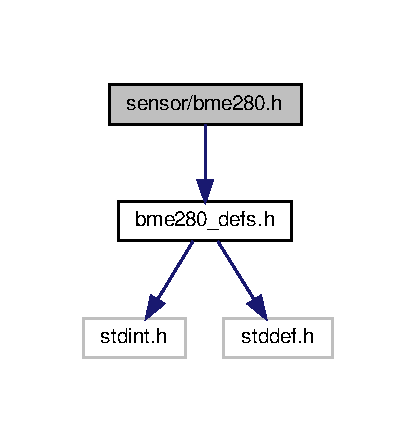
\includegraphics[width=200pt]{bme280_8h__incl}
\end{center}
\end{figure}
This graph shows which files directly or indirectly include this file\+:
\nopagebreak
\begin{figure}[H]
\begin{center}
\leavevmode
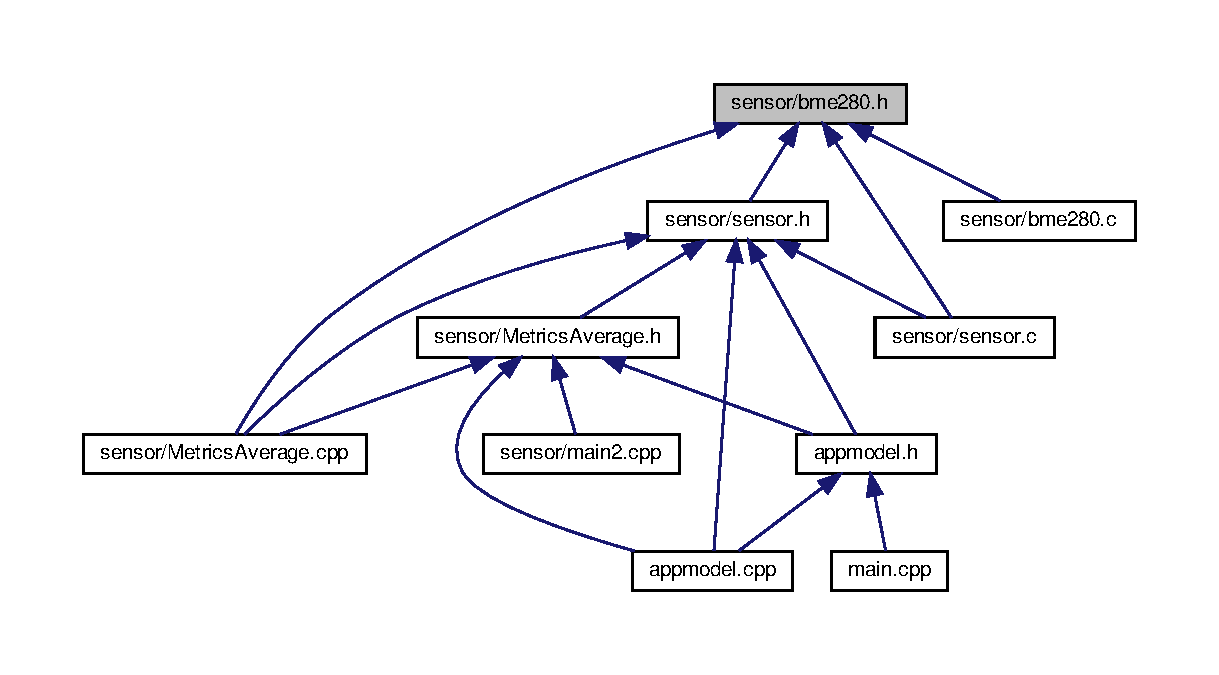
\includegraphics[width=350pt]{bme280_8h__dep__incl}
\end{center}
\end{figure}
\subsection*{Functions}
\begin{DoxyCompactItemize}
\item 
int8\+\_\+t \hyperlink{group___b_m_e280_gaf0b7d7a19bb48ec9eb3651b79f0c3e85}{bme280\+\_\+init} (struct \hyperlink{structbme280__dev}{bme280\+\_\+dev} $\ast$dev)
\begin{DoxyCompactList}\small\item\em This A\+PI is the entry point. It reads the chip-\/id and calibration data from the sensor. \end{DoxyCompactList}\item 
int8\+\_\+t \hyperlink{group___b_m_e280_ga002175df0ebe7893fcf0a54dfe806ba1}{bme280\+\_\+set\+\_\+regs} (uint8\+\_\+t $\ast$reg\+\_\+addr, const uint8\+\_\+t $\ast$reg\+\_\+data, uint8\+\_\+t len, const struct \hyperlink{structbme280__dev}{bme280\+\_\+dev} $\ast$dev)
\begin{DoxyCompactList}\small\item\em This A\+PI writes the given data to the register address of the sensor. \end{DoxyCompactList}\item 
int8\+\_\+t \hyperlink{group___b_m_e280_ga992c5a438b414fe4724764738b88d9d7}{bme280\+\_\+get\+\_\+regs} (uint8\+\_\+t reg\+\_\+addr, uint8\+\_\+t $\ast$reg\+\_\+data, uint16\+\_\+t len, const struct \hyperlink{structbme280__dev}{bme280\+\_\+dev} $\ast$dev)
\begin{DoxyCompactList}\small\item\em This A\+PI reads the data from the given register address of the sensor. \end{DoxyCompactList}\item 
int8\+\_\+t \hyperlink{group___b_m_e280_ga5d436d907394fde22471347599948205}{bme280\+\_\+set\+\_\+sensor\+\_\+settings} (uint8\+\_\+t desired\+\_\+settings, const struct \hyperlink{structbme280__dev}{bme280\+\_\+dev} $\ast$dev)
\begin{DoxyCompactList}\small\item\em This A\+PI sets the oversampling, filter and standby duration (normal mode) settings in the sensor. \end{DoxyCompactList}\item 
int8\+\_\+t \hyperlink{group___b_m_e280_gaf3bef90d33942197a98715ea8657211f}{bme280\+\_\+get\+\_\+sensor\+\_\+settings} (struct \hyperlink{structbme280__dev}{bme280\+\_\+dev} $\ast$dev)
\begin{DoxyCompactList}\small\item\em This A\+PI gets the oversampling, filter and standby duration (normal mode) settings from the sensor. \end{DoxyCompactList}\item 
int8\+\_\+t \hyperlink{group___b_m_e280_ga17a0eaeb97e43233af3e6aac8bd426d4}{bme280\+\_\+set\+\_\+sensor\+\_\+mode} (uint8\+\_\+t sensor\+\_\+mode, const struct \hyperlink{structbme280__dev}{bme280\+\_\+dev} $\ast$dev)
\begin{DoxyCompactList}\small\item\em This A\+PI sets the power mode of the sensor. \end{DoxyCompactList}\item 
int8\+\_\+t \hyperlink{group___b_m_e280_ga4e9e8d290d842abb3262591ff9f64bc4}{bme280\+\_\+get\+\_\+sensor\+\_\+mode} (uint8\+\_\+t $\ast$sensor\+\_\+mode, const struct \hyperlink{structbme280__dev}{bme280\+\_\+dev} $\ast$dev)
\begin{DoxyCompactList}\small\item\em This A\+PI gets the power mode of the sensor. \end{DoxyCompactList}\item 
int8\+\_\+t \hyperlink{group___b_m_e280_ga90dd2358e7050455585842a0fd468f97}{bme280\+\_\+soft\+\_\+reset} (const struct \hyperlink{structbme280__dev}{bme280\+\_\+dev} $\ast$dev)
\begin{DoxyCompactList}\small\item\em This A\+PI performs the soft reset of the sensor. \end{DoxyCompactList}\item 
int8\+\_\+t \hyperlink{group___b_m_e280_ga6671fea2c1e01f40029a653b9ab4410d}{bme280\+\_\+get\+\_\+sensor\+\_\+data} (uint8\+\_\+t sensor\+\_\+comp, struct \hyperlink{structbme280__data}{bme280\+\_\+data} $\ast$comp\+\_\+data, struct \hyperlink{structbme280__dev}{bme280\+\_\+dev} $\ast$dev)
\begin{DoxyCompactList}\small\item\em This A\+PI reads the pressure, temperature and humidity data from the sensor, compensates the data and store it in the \hyperlink{structbme280__data}{bme280\+\_\+data} structure instance passed by the user. \end{DoxyCompactList}\item 
void \hyperlink{group___b_m_e280_ga84be45ccf7a3a82138ff2170123462c3}{bme280\+\_\+parse\+\_\+sensor\+\_\+data} (const uint8\+\_\+t $\ast$reg\+\_\+data, struct \hyperlink{structbme280__uncomp__data}{bme280\+\_\+uncomp\+\_\+data} $\ast$uncomp\+\_\+data)
\begin{DoxyCompactList}\small\item\em This A\+PI is used to parse the pressure, temperature and humidity data and store it in the \hyperlink{structbme280__uncomp__data}{bme280\+\_\+uncomp\+\_\+data} structure instance. \end{DoxyCompactList}\item 
int8\+\_\+t \hyperlink{group___b_m_e280_ga9f2c3c8c683b434ca10447515f85c0de}{bme280\+\_\+compensate\+\_\+data} (uint8\+\_\+t sensor\+\_\+comp, const struct \hyperlink{structbme280__uncomp__data}{bme280\+\_\+uncomp\+\_\+data} $\ast$uncomp\+\_\+data, struct \hyperlink{structbme280__data}{bme280\+\_\+data} $\ast$comp\+\_\+data, struct \hyperlink{structbme280__calib__data}{bme280\+\_\+calib\+\_\+data} $\ast$calib\+\_\+data)
\begin{DoxyCompactList}\small\item\em This A\+PI is used to compensate the pressure and/or temperature and/or humidity data according to the component selected by the user. \end{DoxyCompactList}\end{DoxyCompactItemize}


\subsection{Detailed Description}
Sensor driver for B\+M\+E280 sensor. 

Copyright (C) 2016 -\/ 2017 Bosch Sensortec GmbH

Redistribution and use in source and binary forms, with or without modification, are permitted provided that the following conditions are met\+:

Redistributions of source code must retain the above copyright notice, this list of conditions and the following disclaimer.

Redistributions in binary form must reproduce the above copyright notice, this list of conditions and the following disclaimer in the documentation and/or other materials provided with the distribution.

Neither the name of the copyright holder nor the names of the contributors may be used to endorse or promote products derived from this software without specific prior written permission.

T\+H\+IS S\+O\+F\+T\+W\+A\+RE IS P\+R\+O\+V\+I\+D\+ED BY T\+HE C\+O\+P\+Y\+R\+I\+G\+HT H\+O\+L\+D\+E\+RS A\+ND C\+O\+N\+T\+R\+I\+B\+U\+T\+O\+RS \char`\"{}\+A\+S I\+S\char`\"{} A\+ND A\+NY E\+X\+P\+R\+E\+SS OR I\+M\+P\+L\+I\+ED W\+A\+R\+R\+A\+N\+T\+I\+ES, I\+N\+C\+L\+U\+D\+I\+NG, B\+UT N\+OT L\+I\+M\+I\+T\+ED TO, T\+HE I\+M\+P\+L\+I\+ED W\+A\+R\+R\+A\+N\+T\+I\+ES OF M\+E\+R\+C\+H\+A\+N\+T\+A\+B\+I\+L\+I\+TY A\+ND F\+I\+T\+N\+E\+SS F\+OR A P\+A\+R\+T\+I\+C\+U\+L\+AR P\+U\+R\+P\+O\+SE A\+RE D\+I\+S\+C\+L\+A\+I\+M\+ED. IN NO E\+V\+E\+NT S\+H\+A\+LL C\+O\+P\+Y\+R\+I\+G\+HT H\+O\+L\+D\+ER OR C\+O\+N\+T\+R\+I\+B\+U\+T\+O\+RS BE L\+I\+A\+B\+LE F\+OR A\+NY D\+I\+R\+E\+CT, I\+N\+D\+I\+R\+E\+CT, I\+N\+C\+I\+D\+E\+N\+T\+AL, S\+P\+E\+C\+I\+AL, E\+X\+E\+M\+P\+L\+A\+RY, OR C\+O\+N\+S\+E\+Q\+U\+E\+N\+T\+I\+AL D\+A\+M\+A\+G\+ES(I\+N\+C\+L\+U\+D\+I\+NG, B\+UT N\+OT L\+I\+M\+I\+T\+ED TO, P\+R\+O\+C\+U\+R\+E\+M\+E\+NT OF S\+U\+B\+S\+T\+I\+T\+U\+TE G\+O\+O\+DS OR S\+E\+R\+V\+I\+C\+ES; L\+O\+SS OF U\+SE, D\+A\+TA, OR P\+R\+O\+F\+I\+TS; OR B\+U\+S\+I\+N\+E\+SS I\+N\+T\+E\+R\+R\+U\+P\+T\+I\+ON) H\+O\+W\+E\+V\+ER C\+A\+U\+S\+ED A\+ND ON A\+NY T\+H\+E\+O\+RY OF L\+I\+A\+B\+I\+L\+I\+TY, W\+H\+E\+T\+H\+ER IN C\+O\+N\+T\+R\+A\+CT, S\+T\+R\+I\+CT L\+I\+A\+B\+I\+L\+I\+TY, OR T\+O\+RT (I\+N\+C\+L\+U\+D\+I\+NG N\+E\+G\+L\+I\+G\+E\+N\+CE OR O\+T\+H\+E\+R\+W\+I\+SE) A\+R\+I\+S\+I\+NG IN A\+NY W\+AY O\+UT OF T\+HE U\+SE OF T\+H\+IS S\+O\+F\+T\+W\+A\+RE, E\+V\+EN IF A\+D\+V\+I\+S\+ED OF T\+HE P\+O\+S\+S\+I\+B\+I\+L\+I\+TY OF S\+U\+CH D\+A\+M\+A\+GE

The information provided is believed to be accurate and reliable. The copyright holder assumes no responsibility for the consequences of use of such information nor for any infringement of patents or other rights of third parties which may result from its use. No license is granted by implication or otherwise under any patent or patent rights of the copyright holder.

\begin{DoxyDate}{Date}
14 Feb 2018 
\end{DoxyDate}
\begin{DoxyVersion}{Version}
3.\+3.\+4
\end{DoxyVersion}

\hypertarget{bme280__defs_8h}{}\section{sensor/bme280\+\_\+defs.h File Reference}
\label{bme280__defs_8h}\index{sensor/bme280\+\_\+defs.\+h@{sensor/bme280\+\_\+defs.\+h}}


Sensor driver for B\+M\+E280 sensor.  


{\ttfamily \#include $<$stdint.\+h$>$}\newline
{\ttfamily \#include $<$stddef.\+h$>$}\newline
Include dependency graph for bme280\+\_\+defs.\+h\+:
\nopagebreak
\begin{figure}[H]
\begin{center}
\leavevmode
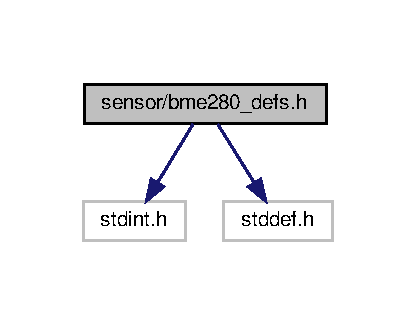
\includegraphics[width=200pt]{bme280__defs_8h__incl}
\end{center}
\end{figure}
This graph shows which files directly or indirectly include this file\+:
\nopagebreak
\begin{figure}[H]
\begin{center}
\leavevmode
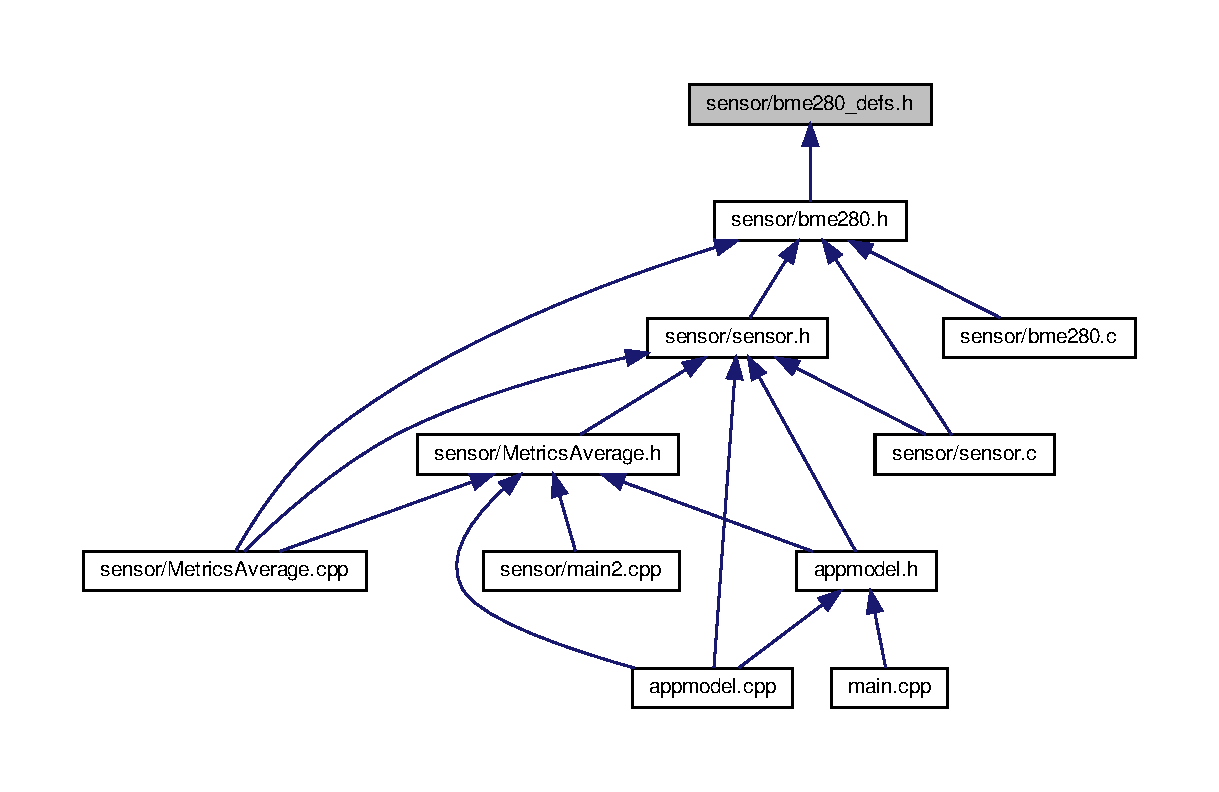
\includegraphics[width=350pt]{bme280__defs_8h__dep__incl}
\end{center}
\end{figure}
\subsection*{Classes}
\begin{DoxyCompactItemize}
\item 
struct \hyperlink{structbme280__calib__data}{bme280\+\_\+calib\+\_\+data}
\begin{DoxyCompactList}\small\item\em Calibration data. \end{DoxyCompactList}\item 
struct \hyperlink{structbme280__data}{bme280\+\_\+data}
\begin{DoxyCompactList}\small\item\em bme280 sensor structure which comprises of temperature, pressure and humidity data \end{DoxyCompactList}\item 
struct \hyperlink{structbme280__uncomp__data}{bme280\+\_\+uncomp\+\_\+data}
\begin{DoxyCompactList}\small\item\em bme280 sensor structure which comprises of uncompensated temperature, pressure and humidity data \end{DoxyCompactList}\item 
struct \hyperlink{structbme280__settings}{bme280\+\_\+settings}
\begin{DoxyCompactList}\small\item\em bme280 sensor settings structure which comprises of mode, oversampling and filter settings. \end{DoxyCompactList}\item 
struct \hyperlink{structbme280__dev}{bme280\+\_\+dev}
\begin{DoxyCompactList}\small\item\em bme280 device structure \end{DoxyCompactList}\end{DoxyCompactItemize}
\subsection*{Macros}
\begin{Indent}\textbf{ Common macros}\par
\begin{DoxyCompactItemize}
\item 
\#define \hyperlink{group___b_m_e280_ga1eaa7db37089dcdfb60227725c9c1585}{I\+N\+T8\+\_\+C}(x)~S8\+\_\+C(x)
\item 
\#define \hyperlink{group___b_m_e280_gacd2aa09844a8a245cf7fdbb808e215e5}{U\+I\+N\+T8\+\_\+C}(x)~U8\+\_\+C(x)
\item 
\#define \hyperlink{group___b_m_e280_ga838b261fec725cb0f5d5b6769d3521e7}{I\+N\+T16\+\_\+C}(x)~S16\+\_\+C(x)
\item 
\#define \hyperlink{group___b_m_e280_ga1cb39a2cfaf899fd38730c7637807708}{U\+I\+N\+T16\+\_\+C}(x)~U16\+\_\+C(x)
\item 
\#define \hyperlink{group___b_m_e280_gad78650fb7726f4e99205406569ef403d}{I\+N\+T32\+\_\+C}(x)~S32\+\_\+C(x)
\item 
\#define \hyperlink{group___b_m_e280_ga2451a7ede7ebd810357f1503e9898ea6}{U\+I\+N\+T32\+\_\+C}(x)~U32\+\_\+C(x)
\item 
\#define \hyperlink{group___b_m_e280_ga93d102802b35d3b8abae9bbe7f0fed75}{I\+N\+T64\+\_\+C}(x)~S64\+\_\+C(x)
\item 
\#define \hyperlink{group___b_m_e280_ga134ae84400d184ed2570e3270d5472c2}{U\+I\+N\+T64\+\_\+C}(x)~U64\+\_\+C(x)
\end{DoxyCompactItemize}
\end{Indent}
\begin{Indent}\textbf{ C standard macros}\par
\begin{DoxyCompactItemize}
\item 
\#define \hyperlink{group___b_m_e280_ga070d2ce7b6bb7e5c05602aa8c308d0c4}{N\+U\+LL}~((void $\ast$) 0)
\item 
\#define \hyperlink{group___b_m_e280_ga1f8aefa20d6054afa77893ea854d9159}{B\+M\+E280\+\_\+\+F\+L\+O\+A\+T\+\_\+\+E\+N\+A\+B\+LE}
\item 
\#define \hyperlink{group___b_m_e280_gaa8cecfc5c5c054d2875c03e77b7be15d}{T\+R\+UE}~\hyperlink{group___b_m_e280_gacd2aa09844a8a245cf7fdbb808e215e5}{U\+I\+N\+T8\+\_\+C}(1)
\item 
\#define \hyperlink{group___b_m_e280_gaa93f0eb578d23995850d61f7d61c55c1}{F\+A\+L\+SE}~\hyperlink{group___b_m_e280_gacd2aa09844a8a245cf7fdbb808e215e5}{U\+I\+N\+T8\+\_\+C}(0)
\end{DoxyCompactItemize}
\end{Indent}
\begin{Indent}\textbf{ I2C addresses}\par
\begin{DoxyCompactItemize}
\item 
\#define \hyperlink{group___b_m_e280_ga34f07b8a4a9b1f48641b131f3dff720c}{B\+M\+E280\+\_\+\+I2\+C\+\_\+\+A\+D\+D\+R\+\_\+\+P\+R\+IM}~\hyperlink{group___b_m_e280_gacd2aa09844a8a245cf7fdbb808e215e5}{U\+I\+N\+T8\+\_\+C}(0x76)
\item 
\#define \hyperlink{group___b_m_e280_gad8bc0d50730a48164ee3a882139e9959}{B\+M\+E280\+\_\+\+I2\+C\+\_\+\+A\+D\+D\+R\+\_\+\+S\+EC}~\hyperlink{group___b_m_e280_gacd2aa09844a8a245cf7fdbb808e215e5}{U\+I\+N\+T8\+\_\+C}(0x77)
\end{DoxyCompactItemize}
\end{Indent}
\begin{Indent}\textbf{ B\+M\+E280 chip identifier}\par
\begin{DoxyCompactItemize}
\item 
\#define \hyperlink{group___b_m_e280_gaa9471d8f9c99880c3b85360017908e6b}{B\+M\+E280\+\_\+\+C\+H\+I\+P\+\_\+\+ID}~\hyperlink{group___b_m_e280_gacd2aa09844a8a245cf7fdbb808e215e5}{U\+I\+N\+T8\+\_\+C}(0x60)
\end{DoxyCompactItemize}
\end{Indent}
\begin{Indent}\textbf{ Register Address}\par
\begin{DoxyCompactItemize}
\item 
\#define \hyperlink{group___b_m_e280_gafc2c2e977533781c8fad2dc1a9408b4e}{B\+M\+E280\+\_\+\+C\+H\+I\+P\+\_\+\+I\+D\+\_\+\+A\+D\+DR}~\hyperlink{group___b_m_e280_gacd2aa09844a8a245cf7fdbb808e215e5}{U\+I\+N\+T8\+\_\+C}(0x\+D0)
\item 
\#define \hyperlink{group___b_m_e280_ga946f939c2dda53735f06cb86abb216e4}{B\+M\+E280\+\_\+\+R\+E\+S\+E\+T\+\_\+\+A\+D\+DR}~\hyperlink{group___b_m_e280_gacd2aa09844a8a245cf7fdbb808e215e5}{U\+I\+N\+T8\+\_\+C}(0x\+E0)
\item 
\#define \hyperlink{group___b_m_e280_ga312afdb80e73c77393ea9aac287b42f5}{B\+M\+E280\+\_\+\+T\+E\+M\+P\+\_\+\+P\+R\+E\+S\+S\+\_\+\+C\+A\+L\+I\+B\+\_\+\+D\+A\+T\+A\+\_\+\+A\+D\+DR}~\hyperlink{group___b_m_e280_gacd2aa09844a8a245cf7fdbb808e215e5}{U\+I\+N\+T8\+\_\+C}(0x88)
\item 
\#define \hyperlink{group___b_m_e280_gab3deba49b93318f0daa9e9aa238d8299}{B\+M\+E280\+\_\+\+H\+U\+M\+I\+D\+I\+T\+Y\+\_\+\+C\+A\+L\+I\+B\+\_\+\+D\+A\+T\+A\+\_\+\+A\+D\+DR}~\hyperlink{group___b_m_e280_gacd2aa09844a8a245cf7fdbb808e215e5}{U\+I\+N\+T8\+\_\+C}(0x\+E1)
\item 
\#define \hyperlink{group___b_m_e280_ga98ddb9dc59edd34aa1d9ea44a05feb7b}{B\+M\+E280\+\_\+\+P\+W\+R\+\_\+\+C\+T\+R\+L\+\_\+\+A\+D\+DR}~\hyperlink{group___b_m_e280_gacd2aa09844a8a245cf7fdbb808e215e5}{U\+I\+N\+T8\+\_\+C}(0x\+F4)
\item 
\#define \hyperlink{group___b_m_e280_ga8f090989bb45d85c2605e4a86a49b46d}{B\+M\+E280\+\_\+\+C\+T\+R\+L\+\_\+\+H\+U\+M\+\_\+\+A\+D\+DR}~\hyperlink{group___b_m_e280_gacd2aa09844a8a245cf7fdbb808e215e5}{U\+I\+N\+T8\+\_\+C}(0x\+F2)
\item 
\#define \hyperlink{group___b_m_e280_ga53b7ccb8b940a9bdd861a7722732c9cc}{B\+M\+E280\+\_\+\+C\+T\+R\+L\+\_\+\+M\+E\+A\+S\+\_\+\+A\+D\+DR}~\hyperlink{group___b_m_e280_gacd2aa09844a8a245cf7fdbb808e215e5}{U\+I\+N\+T8\+\_\+C}(0x\+F4)
\item 
\#define \hyperlink{group___b_m_e280_ga7c2fa57fdeb63ca2c255432f4c98298e}{B\+M\+E280\+\_\+\+C\+O\+N\+F\+I\+G\+\_\+\+A\+D\+DR}~\hyperlink{group___b_m_e280_gacd2aa09844a8a245cf7fdbb808e215e5}{U\+I\+N\+T8\+\_\+C}(0x\+F5)
\item 
\#define \hyperlink{group___b_m_e280_ga1bcfa4087dcd9ca9af43fce23de8eaf2}{B\+M\+E280\+\_\+\+D\+A\+T\+A\+\_\+\+A\+D\+DR}~\hyperlink{group___b_m_e280_gacd2aa09844a8a245cf7fdbb808e215e5}{U\+I\+N\+T8\+\_\+C}(0x\+F7)
\end{DoxyCompactItemize}
\end{Indent}
\begin{Indent}\textbf{ A\+PI success code}\par
\begin{DoxyCompactItemize}
\item 
\#define \hyperlink{group___b_m_e280_gabfe3dd12ee6f5f5d51fbb340a22ff678}{B\+M\+E280\+\_\+\+OK}~\hyperlink{group___b_m_e280_ga1eaa7db37089dcdfb60227725c9c1585}{I\+N\+T8\+\_\+C}(0)
\end{DoxyCompactItemize}
\end{Indent}
\begin{Indent}\textbf{ A\+PI error codes}\par
\begin{DoxyCompactItemize}
\item 
\#define \hyperlink{group___b_m_e280_ga269f65e4816ca679d618175efefcb00d}{B\+M\+E280\+\_\+\+E\+\_\+\+N\+U\+L\+L\+\_\+\+P\+TR}~\hyperlink{group___b_m_e280_ga1eaa7db37089dcdfb60227725c9c1585}{I\+N\+T8\+\_\+C}(-\/1)
\item 
\#define \hyperlink{group___b_m_e280_ga0be1b2946c861fe3e3212e14bb9762a0}{B\+M\+E280\+\_\+\+E\+\_\+\+D\+E\+V\+\_\+\+N\+O\+T\+\_\+\+F\+O\+U\+ND}~\hyperlink{group___b_m_e280_ga1eaa7db37089dcdfb60227725c9c1585}{I\+N\+T8\+\_\+C}(-\/2)
\item 
\#define \hyperlink{group___b_m_e280_gafeb74eb5e3f125d1f03be173e40c89b0}{B\+M\+E280\+\_\+\+E\+\_\+\+I\+N\+V\+A\+L\+I\+D\+\_\+\+L\+EN}~\hyperlink{group___b_m_e280_ga1eaa7db37089dcdfb60227725c9c1585}{I\+N\+T8\+\_\+C}(-\/3)
\item 
\#define \hyperlink{group___b_m_e280_ga2b47776b53e3167b0068bc6ef21f1523}{B\+M\+E280\+\_\+\+E\+\_\+\+C\+O\+M\+M\+\_\+\+F\+A\+IL}~\hyperlink{group___b_m_e280_ga1eaa7db37089dcdfb60227725c9c1585}{I\+N\+T8\+\_\+C}(-\/4)
\item 
\#define \hyperlink{group___b_m_e280_ga2de574b1e957addef1056b59ec7502d5}{B\+M\+E280\+\_\+\+E\+\_\+\+S\+L\+E\+E\+P\+\_\+\+M\+O\+D\+E\+\_\+\+F\+A\+IL}~\hyperlink{group___b_m_e280_ga1eaa7db37089dcdfb60227725c9c1585}{I\+N\+T8\+\_\+C}(-\/5)
\end{DoxyCompactItemize}
\end{Indent}
\begin{Indent}\textbf{ A\+PI warning codes}\par
\begin{DoxyCompactItemize}
\item 
\#define \hyperlink{group___b_m_e280_ga14e40d625ed338734e57fbc434ca5723}{B\+M\+E280\+\_\+\+W\+\_\+\+I\+N\+V\+A\+L\+I\+D\+\_\+\+O\+S\+R\+\_\+\+M\+A\+C\+RO}~\hyperlink{group___b_m_e280_ga1eaa7db37089dcdfb60227725c9c1585}{I\+N\+T8\+\_\+C}(1)
\end{DoxyCompactItemize}
\end{Indent}
\begin{Indent}\textbf{ Macros related to size}\par
\begin{DoxyCompactItemize}
\item 
\#define \hyperlink{group___b_m_e280_gab44aa25677fa7fcab0a4ccc59b050286}{B\+M\+E280\+\_\+\+T\+E\+M\+P\+\_\+\+P\+R\+E\+S\+S\+\_\+\+C\+A\+L\+I\+B\+\_\+\+D\+A\+T\+A\+\_\+\+L\+EN}~\hyperlink{group___b_m_e280_gacd2aa09844a8a245cf7fdbb808e215e5}{U\+I\+N\+T8\+\_\+C}(26)
\item 
\#define \hyperlink{group___b_m_e280_ga3768333f53ae57f3047838552e7771d5}{B\+M\+E280\+\_\+\+H\+U\+M\+I\+D\+I\+T\+Y\+\_\+\+C\+A\+L\+I\+B\+\_\+\+D\+A\+T\+A\+\_\+\+L\+EN}~\hyperlink{group___b_m_e280_gacd2aa09844a8a245cf7fdbb808e215e5}{U\+I\+N\+T8\+\_\+C}(7)
\item 
\#define \hyperlink{group___b_m_e280_gaf4fd5bc6f8cc635fe961cc20acfcbe5c}{B\+M\+E280\+\_\+\+P\+\_\+\+T\+\_\+\+H\+\_\+\+D\+A\+T\+A\+\_\+\+L\+EN}~\hyperlink{group___b_m_e280_gacd2aa09844a8a245cf7fdbb808e215e5}{U\+I\+N\+T8\+\_\+C}(8)
\end{DoxyCompactItemize}
\end{Indent}
\begin{Indent}\textbf{ Sensor power modes}\par
\begin{DoxyCompactItemize}
\item 
\#define \hyperlink{group___b_m_e280_ga4db27e6a138fa0ba5c2f5779467b5871}{B\+M\+E280\+\_\+\+S\+L\+E\+E\+P\+\_\+\+M\+O\+DE}~\hyperlink{group___b_m_e280_gacd2aa09844a8a245cf7fdbb808e215e5}{U\+I\+N\+T8\+\_\+C}(0x00)
\item 
\#define \hyperlink{group___b_m_e280_gae59bb15caa6e0a75e373286eacb5abc4}{B\+M\+E280\+\_\+\+F\+O\+R\+C\+E\+D\+\_\+\+M\+O\+DE}~\hyperlink{group___b_m_e280_gacd2aa09844a8a245cf7fdbb808e215e5}{U\+I\+N\+T8\+\_\+C}(0x01)
\item 
\#define \hyperlink{group___b_m_e280_ga8a9c2aa9289d646803badb7d7fdbd5cb}{B\+M\+E280\+\_\+\+N\+O\+R\+M\+A\+L\+\_\+\+M\+O\+DE}~\hyperlink{group___b_m_e280_gacd2aa09844a8a245cf7fdbb808e215e5}{U\+I\+N\+T8\+\_\+C}(0x03)
\end{DoxyCompactItemize}
\end{Indent}
\begin{Indent}\textbf{ Macro to combine two 8 bit data\textquotesingle{}s to form a 16 bit data}\par
\begin{DoxyCompactItemize}
\item 
\#define \hyperlink{group___b_m_e280_ga0202d632129238d5f788e362c19ccf93}{B\+M\+E280\+\_\+\+C\+O\+N\+C\+A\+T\+\_\+\+B\+Y\+T\+ES}(msb,  lsb)~(((uint16\+\_\+t)msb $<$$<$ 8) $\vert$ (uint16\+\_\+t)lsb)
\item 
\#define \hyperlink{group___b_m_e280_ga78f60fe8571e15f6a21ba8fcaa12e0ce}{B\+M\+E280\+\_\+\+S\+E\+T\+\_\+\+B\+I\+TS}(reg\+\_\+data,  bitname,  \hyperlink{structdata}{data})
\item 
\#define \hyperlink{group___b_m_e280_ga72c20c06b3a42de7660bf1d8678cd645}{B\+M\+E280\+\_\+\+S\+E\+T\+\_\+\+B\+I\+T\+S\+\_\+\+P\+O\+S\+\_\+0}(reg\+\_\+data,  bitname,  \hyperlink{structdata}{data})
\item 
\#define \hyperlink{group___b_m_e280_gaa28698af242be4e59a2812ebe4165982}{B\+M\+E280\+\_\+\+G\+E\+T\+\_\+\+B\+I\+TS}(reg\+\_\+data,  bitname)
\item 
\#define \hyperlink{group___b_m_e280_ga2c4248bc9b39a806aca49e34b1a5636c}{B\+M\+E280\+\_\+\+G\+E\+T\+\_\+\+B\+I\+T\+S\+\_\+\+P\+O\+S\+\_\+0}(reg\+\_\+data,  bitname)~(reg\+\_\+data \& (bitname\#\#\+\_\+\+M\+SK))
\end{DoxyCompactItemize}
\end{Indent}
\begin{Indent}\textbf{ Macros for bit masking}\par
\begin{DoxyCompactItemize}
\item 
\#define \hyperlink{group___b_m_e280_gaa8dbb21db223923e34d32c285a2a6660}{B\+M\+E280\+\_\+\+S\+E\+N\+S\+O\+R\+\_\+\+M\+O\+D\+E\+\_\+\+M\+SK}~\hyperlink{group___b_m_e280_gacd2aa09844a8a245cf7fdbb808e215e5}{U\+I\+N\+T8\+\_\+C}(0x03)
\item 
\#define \hyperlink{group___b_m_e280_ga20dfd35772ac7aff0f6ba4f0c7d8352e}{B\+M\+E280\+\_\+\+S\+E\+N\+S\+O\+R\+\_\+\+M\+O\+D\+E\+\_\+\+P\+OS}~\hyperlink{group___b_m_e280_gacd2aa09844a8a245cf7fdbb808e215e5}{U\+I\+N\+T8\+\_\+C}(0x00)
\item 
\#define \hyperlink{group___b_m_e280_gaf0b6595ecc184d00b061d06cc14b9a29}{B\+M\+E280\+\_\+\+C\+T\+R\+L\+\_\+\+H\+U\+M\+\_\+\+M\+SK}~\hyperlink{group___b_m_e280_gacd2aa09844a8a245cf7fdbb808e215e5}{U\+I\+N\+T8\+\_\+C}(0x07)
\item 
\#define \hyperlink{group___b_m_e280_ga90412039a144a430b9e6aeff23b63665}{B\+M\+E280\+\_\+\+C\+T\+R\+L\+\_\+\+H\+U\+M\+\_\+\+P\+OS}~\hyperlink{group___b_m_e280_gacd2aa09844a8a245cf7fdbb808e215e5}{U\+I\+N\+T8\+\_\+C}(0x00)
\item 
\#define \hyperlink{group___b_m_e280_ga579a2e3a1a74b90ccf28e50dae21d6e4}{B\+M\+E280\+\_\+\+C\+T\+R\+L\+\_\+\+P\+R\+E\+S\+S\+\_\+\+M\+SK}~\hyperlink{group___b_m_e280_gacd2aa09844a8a245cf7fdbb808e215e5}{U\+I\+N\+T8\+\_\+C}(0x1\+C)
\item 
\#define \hyperlink{group___b_m_e280_gaaed4e0278b7c828ed24100640a2d9a82}{B\+M\+E280\+\_\+\+C\+T\+R\+L\+\_\+\+P\+R\+E\+S\+S\+\_\+\+P\+OS}~\hyperlink{group___b_m_e280_gacd2aa09844a8a245cf7fdbb808e215e5}{U\+I\+N\+T8\+\_\+C}(0x02)
\item 
\#define \hyperlink{group___b_m_e280_gaf7371331e2fa7adb92322120ace956c2}{B\+M\+E280\+\_\+\+C\+T\+R\+L\+\_\+\+T\+E\+M\+P\+\_\+\+M\+SK}~\hyperlink{group___b_m_e280_gacd2aa09844a8a245cf7fdbb808e215e5}{U\+I\+N\+T8\+\_\+C}(0x\+E0)
\item 
\#define \hyperlink{group___b_m_e280_gae8c4ff4ea9185b90c3bd26a9e51c9ad9}{B\+M\+E280\+\_\+\+C\+T\+R\+L\+\_\+\+T\+E\+M\+P\+\_\+\+P\+OS}~\hyperlink{group___b_m_e280_gacd2aa09844a8a245cf7fdbb808e215e5}{U\+I\+N\+T8\+\_\+C}(0x05)
\item 
\#define \hyperlink{group___b_m_e280_ga2987fc2cac045851392c6be3adc97321}{B\+M\+E280\+\_\+\+F\+I\+L\+T\+E\+R\+\_\+\+M\+SK}~\hyperlink{group___b_m_e280_gacd2aa09844a8a245cf7fdbb808e215e5}{U\+I\+N\+T8\+\_\+C}(0x1\+C)
\item 
\#define \hyperlink{group___b_m_e280_gaa1b84aa73f4208ec8bc348f0befd6218}{B\+M\+E280\+\_\+\+F\+I\+L\+T\+E\+R\+\_\+\+P\+OS}~\hyperlink{group___b_m_e280_gacd2aa09844a8a245cf7fdbb808e215e5}{U\+I\+N\+T8\+\_\+C}(0x02)
\item 
\#define \hyperlink{group___b_m_e280_gad605c1d49d0c13cc7fd78148894c8be3}{B\+M\+E280\+\_\+\+S\+T\+A\+N\+D\+B\+Y\+\_\+\+M\+SK}~\hyperlink{group___b_m_e280_gacd2aa09844a8a245cf7fdbb808e215e5}{U\+I\+N\+T8\+\_\+C}(0x\+E0)
\item 
\#define \hyperlink{group___b_m_e280_ga95d6cbf0004b76308440a9b72d157508}{B\+M\+E280\+\_\+\+S\+T\+A\+N\+D\+B\+Y\+\_\+\+P\+OS}~\hyperlink{group___b_m_e280_gacd2aa09844a8a245cf7fdbb808e215e5}{U\+I\+N\+T8\+\_\+C}(0x05)
\end{DoxyCompactItemize}
\end{Indent}
\begin{Indent}\textbf{ Sensor component selection macros}\par
{\em These values are internal for A\+PI implementation. Don\textquotesingle{}t relate this to data sheet. }\begin{DoxyCompactItemize}
\item 
\#define \hyperlink{group___b_m_e280_gadfbc93f23e81f44aeb31d6e1c3e29f59}{B\+M\+E280\+\_\+\+P\+R\+E\+SS}~\hyperlink{group___b_m_e280_gacd2aa09844a8a245cf7fdbb808e215e5}{U\+I\+N\+T8\+\_\+C}(1)
\item 
\#define \hyperlink{group___b_m_e280_gaa3ffc130a1db4dd1cdb4b11936a2becc}{B\+M\+E280\+\_\+\+T\+E\+MP}~\hyperlink{group___b_m_e280_gacd2aa09844a8a245cf7fdbb808e215e5}{U\+I\+N\+T8\+\_\+C}(1 $<$$<$ 1)
\item 
\#define \hyperlink{group___b_m_e280_ga709c35c30ebfe237189e533dedbca264}{B\+M\+E280\+\_\+\+H\+UM}~\hyperlink{group___b_m_e280_gacd2aa09844a8a245cf7fdbb808e215e5}{U\+I\+N\+T8\+\_\+C}(1 $<$$<$ 2)
\item 
\#define \hyperlink{group___b_m_e280_ga8b1cf23a873282113bb8218e615855e3}{B\+M\+E280\+\_\+\+A\+LL}~\hyperlink{group___b_m_e280_gacd2aa09844a8a245cf7fdbb808e215e5}{U\+I\+N\+T8\+\_\+C}(0x07)
\end{DoxyCompactItemize}
\end{Indent}
\begin{Indent}\textbf{ Settings selection macros}\par
\begin{DoxyCompactItemize}
\item 
\#define \hyperlink{group___b_m_e280_gae22bd3e6b1bb71fe30633f4d84168750}{B\+M\+E280\+\_\+\+O\+S\+R\+\_\+\+P\+R\+E\+S\+S\+\_\+\+S\+EL}~\hyperlink{group___b_m_e280_gacd2aa09844a8a245cf7fdbb808e215e5}{U\+I\+N\+T8\+\_\+C}(1)
\item 
\#define \hyperlink{group___b_m_e280_ga407647f6182e1bd2338e226ea0ef93af}{B\+M\+E280\+\_\+\+O\+S\+R\+\_\+\+T\+E\+M\+P\+\_\+\+S\+EL}~\hyperlink{group___b_m_e280_gacd2aa09844a8a245cf7fdbb808e215e5}{U\+I\+N\+T8\+\_\+C}(1 $<$$<$ 1)
\item 
\#define \hyperlink{group___b_m_e280_gacdab9f807404ce931f3ec87b680986ba}{B\+M\+E280\+\_\+\+O\+S\+R\+\_\+\+H\+U\+M\+\_\+\+S\+EL}~\hyperlink{group___b_m_e280_gacd2aa09844a8a245cf7fdbb808e215e5}{U\+I\+N\+T8\+\_\+C}(1 $<$$<$ 2)
\item 
\#define \hyperlink{group___b_m_e280_ga9d10214add03956eb741957acb90083e}{B\+M\+E280\+\_\+\+F\+I\+L\+T\+E\+R\+\_\+\+S\+EL}~\hyperlink{group___b_m_e280_gacd2aa09844a8a245cf7fdbb808e215e5}{U\+I\+N\+T8\+\_\+C}(1 $<$$<$ 3)
\item 
\#define \hyperlink{group___b_m_e280_gafa104771609eec5766a2f0794fc4374b}{B\+M\+E280\+\_\+\+S\+T\+A\+N\+D\+B\+Y\+\_\+\+S\+EL}~\hyperlink{group___b_m_e280_gacd2aa09844a8a245cf7fdbb808e215e5}{U\+I\+N\+T8\+\_\+C}(1 $<$$<$ 4)
\item 
\#define \hyperlink{group___b_m_e280_ga8ef4306eed189332ad4c4db8003132c8}{B\+M\+E280\+\_\+\+A\+L\+L\+\_\+\+S\+E\+T\+T\+I\+N\+G\+S\+\_\+\+S\+EL}~\hyperlink{group___b_m_e280_gacd2aa09844a8a245cf7fdbb808e215e5}{U\+I\+N\+T8\+\_\+C}(0x1\+F)
\end{DoxyCompactItemize}
\end{Indent}
\begin{Indent}\textbf{ Oversampling macros}\par
\begin{DoxyCompactItemize}
\item 
\#define \hyperlink{group___b_m_e280_ga58004a62b46ed7bcdb8d73ad4fa8cbc1}{B\+M\+E280\+\_\+\+N\+O\+\_\+\+O\+V\+E\+R\+S\+A\+M\+P\+L\+I\+NG}~\hyperlink{group___b_m_e280_gacd2aa09844a8a245cf7fdbb808e215e5}{U\+I\+N\+T8\+\_\+C}(0x00)
\item 
\#define \hyperlink{group___b_m_e280_ga701285fd2495e391411b694c9b50c08a}{B\+M\+E280\+\_\+\+O\+V\+E\+R\+S\+A\+M\+P\+L\+I\+N\+G\+\_\+1X}~\hyperlink{group___b_m_e280_gacd2aa09844a8a245cf7fdbb808e215e5}{U\+I\+N\+T8\+\_\+C}(0x01)
\item 
\#define \hyperlink{group___b_m_e280_ga59a76b60316ed9a11ac552085f33603c}{B\+M\+E280\+\_\+\+O\+V\+E\+R\+S\+A\+M\+P\+L\+I\+N\+G\+\_\+2X}~\hyperlink{group___b_m_e280_gacd2aa09844a8a245cf7fdbb808e215e5}{U\+I\+N\+T8\+\_\+C}(0x02)
\item 
\#define \hyperlink{group___b_m_e280_ga521eb8ad23776eee8faaf58b17191a76}{B\+M\+E280\+\_\+\+O\+V\+E\+R\+S\+A\+M\+P\+L\+I\+N\+G\+\_\+4X}~\hyperlink{group___b_m_e280_gacd2aa09844a8a245cf7fdbb808e215e5}{U\+I\+N\+T8\+\_\+C}(0x03)
\item 
\#define \hyperlink{group___b_m_e280_ga7b3d9cb65ee6dfef65bc1982865c5a90}{B\+M\+E280\+\_\+\+O\+V\+E\+R\+S\+A\+M\+P\+L\+I\+N\+G\+\_\+8X}~\hyperlink{group___b_m_e280_gacd2aa09844a8a245cf7fdbb808e215e5}{U\+I\+N\+T8\+\_\+C}(0x04)
\item 
\#define \hyperlink{group___b_m_e280_gad8dc54a7a7d5bd1fd04d901561f7f646}{B\+M\+E280\+\_\+\+O\+V\+E\+R\+S\+A\+M\+P\+L\+I\+N\+G\+\_\+16X}~\hyperlink{group___b_m_e280_gacd2aa09844a8a245cf7fdbb808e215e5}{U\+I\+N\+T8\+\_\+C}(0x05)
\end{DoxyCompactItemize}
\end{Indent}
\begin{Indent}\textbf{ Standby duration selection macros}\par
\begin{DoxyCompactItemize}
\item 
\#define \hyperlink{group___b_m_e280_ga96007052b64f48620c27a4b929d7b0c5}{B\+M\+E280\+\_\+\+S\+T\+A\+N\+D\+B\+Y\+\_\+\+T\+I\+M\+E\+\_\+1\+\_\+\+MS}~(0x00)
\item 
\#define \hyperlink{group___b_m_e280_ga08d610ade362b9a865fc126189110f96}{B\+M\+E280\+\_\+\+S\+T\+A\+N\+D\+B\+Y\+\_\+\+T\+I\+M\+E\+\_\+62\+\_\+5\+\_\+\+MS}~(0x01)
\item 
\#define \hyperlink{group___b_m_e280_gabda2854c877d0ab552b0d3a5e92ce06a}{B\+M\+E280\+\_\+\+S\+T\+A\+N\+D\+B\+Y\+\_\+\+T\+I\+M\+E\+\_\+125\+\_\+\+MS}~(0x02)
\item 
\#define \hyperlink{group___b_m_e280_ga3c7744e622d09172d4c6fe19d5060901}{B\+M\+E280\+\_\+\+S\+T\+A\+N\+D\+B\+Y\+\_\+\+T\+I\+M\+E\+\_\+250\+\_\+\+MS}~(0x03)
\item 
\#define \hyperlink{group___b_m_e280_ga822d215c13193c2e88010c2c911a1e7c}{B\+M\+E280\+\_\+\+S\+T\+A\+N\+D\+B\+Y\+\_\+\+T\+I\+M\+E\+\_\+500\+\_\+\+MS}~(0x04)
\item 
\#define \hyperlink{group___b_m_e280_gafe13ba4269e78b8a5b2463fbff88fdc9}{B\+M\+E280\+\_\+\+S\+T\+A\+N\+D\+B\+Y\+\_\+\+T\+I\+M\+E\+\_\+1000\+\_\+\+MS}~(0x05)
\item 
\#define \hyperlink{group___b_m_e280_ga2d9584d45556539af37055d1cee375df}{B\+M\+E280\+\_\+\+S\+T\+A\+N\+D\+B\+Y\+\_\+\+T\+I\+M\+E\+\_\+10\+\_\+\+MS}~(0x06)
\item 
\#define \hyperlink{group___b_m_e280_gae9926694b90ad9154a2c849a7bceb7f6}{B\+M\+E280\+\_\+\+S\+T\+A\+N\+D\+B\+Y\+\_\+\+T\+I\+M\+E\+\_\+20\+\_\+\+MS}~(0x07)
\end{DoxyCompactItemize}
\end{Indent}
\subsection*{Filter coefficient selection macros}
\begin{DoxyCompactItemize}
\item 
\#define \hyperlink{group___b_m_e280_gae61c58ec304b87f6f9726992af323dc3}{B\+M\+E280\+\_\+\+F\+I\+L\+T\+E\+R\+\_\+\+C\+O\+E\+F\+F\+\_\+\+O\+FF}~(0x00)
\item 
\#define \hyperlink{group___b_m_e280_ga225fa757613310b9dfd1cb83cfe71080}{B\+M\+E280\+\_\+\+F\+I\+L\+T\+E\+R\+\_\+\+C\+O\+E\+F\+F\+\_\+2}~(0x01)
\item 
\#define \hyperlink{group___b_m_e280_ga75df0ff360627c3efdd98ad38a92dab0}{B\+M\+E280\+\_\+\+F\+I\+L\+T\+E\+R\+\_\+\+C\+O\+E\+F\+F\+\_\+4}~(0x02)
\item 
\#define \hyperlink{group___b_m_e280_gae6f638d18f380c7e537c02c7bb1a6c22}{B\+M\+E280\+\_\+\+F\+I\+L\+T\+E\+R\+\_\+\+C\+O\+E\+F\+F\+\_\+8}~(0x03)
\item 
\#define \hyperlink{group___b_m_e280_ga73ced29de70a4fe0fa1f05676b2604e4}{B\+M\+E280\+\_\+\+F\+I\+L\+T\+E\+R\+\_\+\+C\+O\+E\+F\+F\+\_\+16}~(0x04)
\item 
enum \hyperlink{group___b_m_e280_ga142fcd9cb1e99b793488e9b3b1e6766e}{bme280\+\_\+intf} \{ \hyperlink{group___b_m_e280_gga142fcd9cb1e99b793488e9b3b1e6766eab5516f6eca9b94ae116261c33c388f4c}{B\+M\+E280\+\_\+\+S\+P\+I\+\_\+\+I\+N\+TF}, 
\hyperlink{group___b_m_e280_gga142fcd9cb1e99b793488e9b3b1e6766eaae41ddfd32babefbce48e7b7671f46a2}{B\+M\+E280\+\_\+\+I2\+C\+\_\+\+I\+N\+TF}
 \}\begin{DoxyCompactList}\small\item\em Interface selection Enums. \end{DoxyCompactList}
\item 
typedef int8\+\_\+t($\ast$ \hyperlink{group___b_m_e280_ga7c23fe68ccf92adb3f03882b40739e7b}{bme280\+\_\+com\+\_\+fptr\+\_\+t}) (uint8\+\_\+t dev\+\_\+id, uint8\+\_\+t reg\+\_\+addr, uint8\+\_\+t $\ast$\hyperlink{structdata}{data}, uint16\+\_\+t len)
\begin{DoxyCompactList}\small\item\em Type definitions. \end{DoxyCompactList}\item 
typedef void($\ast$ \hyperlink{group___b_m_e280_gab2783d9a00e56ddc3e0e8d37b3462e34}{bme280\+\_\+delay\+\_\+fptr\+\_\+t}) (uint32\+\_\+t period)
\end{DoxyCompactItemize}


\subsection{Detailed Description}
Sensor driver for B\+M\+E280 sensor. 

Copyright (C) 2016 -\/ 2017 Bosch Sensortec GmbH

Redistribution and use in source and binary forms, with or without modification, are permitted provided that the following conditions are met\+:

Redistributions of source code must retain the above copyright notice, this list of conditions and the following disclaimer.

Redistributions in binary form must reproduce the above copyright notice, this list of conditions and the following disclaimer in the documentation and/or other materials provided with the distribution.

Neither the name of the copyright holder nor the names of the contributors may be used to endorse or promote products derived from this software without specific prior written permission.

T\+H\+IS S\+O\+F\+T\+W\+A\+RE IS P\+R\+O\+V\+I\+D\+ED BY T\+HE C\+O\+P\+Y\+R\+I\+G\+HT H\+O\+L\+D\+E\+RS A\+ND C\+O\+N\+T\+R\+I\+B\+U\+T\+O\+RS \char`\"{}\+A\+S I\+S\char`\"{} A\+ND A\+NY E\+X\+P\+R\+E\+SS OR I\+M\+P\+L\+I\+ED W\+A\+R\+R\+A\+N\+T\+I\+ES, I\+N\+C\+L\+U\+D\+I\+NG, B\+UT N\+OT L\+I\+M\+I\+T\+ED TO, T\+HE I\+M\+P\+L\+I\+ED W\+A\+R\+R\+A\+N\+T\+I\+ES OF M\+E\+R\+C\+H\+A\+N\+T\+A\+B\+I\+L\+I\+TY A\+ND F\+I\+T\+N\+E\+SS F\+OR A P\+A\+R\+T\+I\+C\+U\+L\+AR P\+U\+R\+P\+O\+SE A\+RE D\+I\+S\+C\+L\+A\+I\+M\+ED. IN NO E\+V\+E\+NT S\+H\+A\+LL C\+O\+P\+Y\+R\+I\+G\+HT H\+O\+L\+D\+ER OR C\+O\+N\+T\+R\+I\+B\+U\+T\+O\+RS BE L\+I\+A\+B\+LE F\+OR A\+NY D\+I\+R\+E\+CT, I\+N\+D\+I\+R\+E\+CT, I\+N\+C\+I\+D\+E\+N\+T\+AL, S\+P\+E\+C\+I\+AL, E\+X\+E\+M\+P\+L\+A\+RY, OR C\+O\+N\+S\+E\+Q\+U\+E\+N\+T\+I\+AL D\+A\+M\+A\+G\+ES(I\+N\+C\+L\+U\+D\+I\+NG, B\+UT N\+OT L\+I\+M\+I\+T\+ED TO, P\+R\+O\+C\+U\+R\+E\+M\+E\+NT OF S\+U\+B\+S\+T\+I\+T\+U\+TE G\+O\+O\+DS OR S\+E\+R\+V\+I\+C\+ES; L\+O\+SS OF U\+SE, D\+A\+TA, OR P\+R\+O\+F\+I\+TS; OR B\+U\+S\+I\+N\+E\+SS I\+N\+T\+E\+R\+R\+U\+P\+T\+I\+ON) H\+O\+W\+E\+V\+ER C\+A\+U\+S\+ED A\+ND ON A\+NY T\+H\+E\+O\+RY OF L\+I\+A\+B\+I\+L\+I\+TY, W\+H\+E\+T\+H\+ER IN C\+O\+N\+T\+R\+A\+CT, S\+T\+R\+I\+CT L\+I\+A\+B\+I\+L\+I\+TY, OR T\+O\+RT (I\+N\+C\+L\+U\+D\+I\+NG N\+E\+G\+L\+I\+G\+E\+N\+CE OR O\+T\+H\+E\+R\+W\+I\+SE) A\+R\+I\+S\+I\+NG IN A\+NY W\+AY O\+UT OF T\+HE U\+SE OF T\+H\+IS S\+O\+F\+T\+W\+A\+RE, E\+V\+EN IF A\+D\+V\+I\+S\+ED OF T\+HE P\+O\+S\+S\+I\+B\+I\+L\+I\+TY OF S\+U\+CH D\+A\+M\+A\+GE

The information provided is believed to be accurate and reliable. The copyright holder assumes no responsibility for the consequences of use of such information nor for any infringement of patents or other rights of third parties which may result from its use. No license is granted by implication or otherwise under any patent or patent rights of the copyright holder.

\begin{DoxyDate}{Date}
14 Feb 2018 
\end{DoxyDate}
\begin{DoxyVersion}{Version}
3.\+3.\+4
\end{DoxyVersion}

\hypertarget{main2_8cpp}{}\section{sensor/main2.cpp File Reference}
\label{main2_8cpp}\index{sensor/main2.\+cpp@{sensor/main2.\+cpp}}
{\ttfamily \#include $<$time.\+h$>$}\newline
{\ttfamily \#include \char`\"{}Metrics\+Average.\+h\char`\"{}}\newline
{\ttfamily \#include $<$string$>$}\newline
{\ttfamily \#include $<$iostream$>$}\newline
Include dependency graph for main2.\+cpp\+:
\nopagebreak
\begin{figure}[H]
\begin{center}
\leavevmode
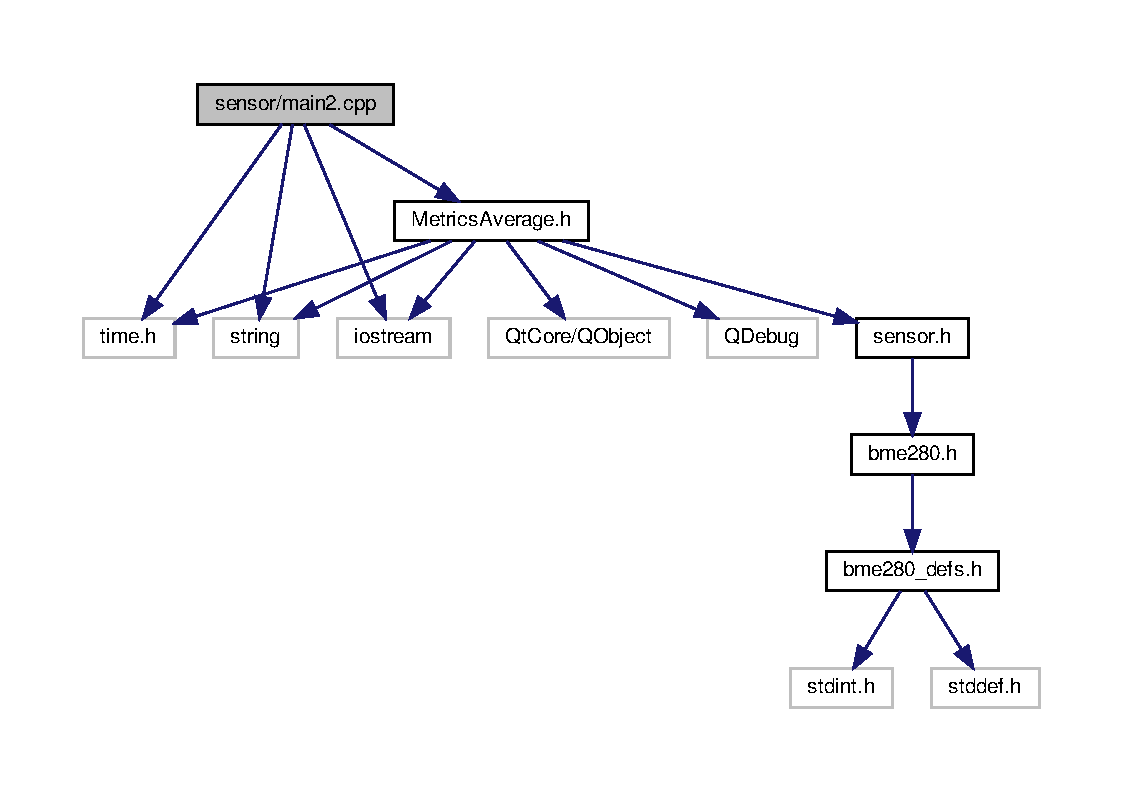
\includegraphics[width=350pt]{main2_8cpp__incl}
\end{center}
\end{figure}
\subsection*{Functions}
\begin{DoxyCompactItemize}
\item 
int \hyperlink{main2_8cpp_ae66f6b31b5ad750f1fe042a706a4e3d4}{main} ()
\end{DoxyCompactItemize}


\subsection{Function Documentation}
\mbox{\Hypertarget{main2_8cpp_ae66f6b31b5ad750f1fe042a706a4e3d4}\label{main2_8cpp_ae66f6b31b5ad750f1fe042a706a4e3d4}} 
\index{main2.\+cpp@{main2.\+cpp}!main@{main}}
\index{main@{main}!main2.\+cpp@{main2.\+cpp}}
\subsubsection{\texorpdfstring{main()}{main()}}
{\footnotesize\ttfamily int main (\begin{DoxyParamCaption}\item[{void}]{ }\end{DoxyParamCaption})}


\hypertarget{_metrics_average_8cpp}{}\section{sensor/\+Metrics\+Average.cpp File Reference}
\label{_metrics_average_8cpp}\index{sensor/\+Metrics\+Average.\+cpp@{sensor/\+Metrics\+Average.\+cpp}}
{\ttfamily \#include \char`\"{}Metrics\+Average.\+h\char`\"{}}\newline
{\ttfamily \#include $<$string$>$}\newline
{\ttfamily \#include $<$time.\+h$>$}\newline
{\ttfamily \#include $<$iostream$>$}\newline
{\ttfamily \#include \char`\"{}bme280.\+h\char`\"{}}\newline
{\ttfamily \#include \char`\"{}sensor.\+h\char`\"{}}\newline
Include dependency graph for Metrics\+Average.\+cpp\+:
\nopagebreak
\begin{figure}[H]
\begin{center}
\leavevmode
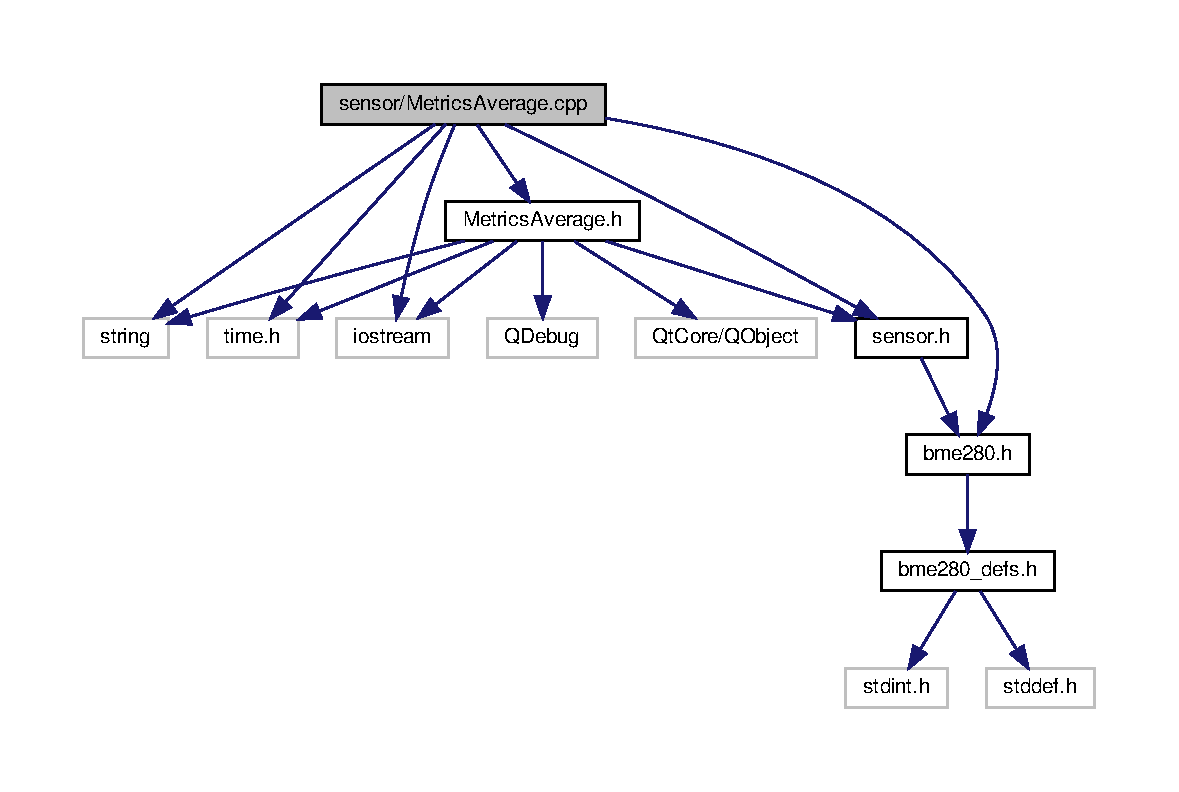
\includegraphics[width=350pt]{_metrics_average_8cpp__incl}
\end{center}
\end{figure}
\subsection*{Variables}
\begin{DoxyCompactItemize}
\item 
struct \hyperlink{structbme280__dev}{bme280\+\_\+dev} \hyperlink{_metrics_average_8cpp_a84ba6c409cfe098d180b2292fd23a843}{g\+\_\+dev}
\end{DoxyCompactItemize}


\subsection{Variable Documentation}
\mbox{\Hypertarget{_metrics_average_8cpp_a84ba6c409cfe098d180b2292fd23a843}\label{_metrics_average_8cpp_a84ba6c409cfe098d180b2292fd23a843}} 
\index{Metrics\+Average.\+cpp@{Metrics\+Average.\+cpp}!g\+\_\+dev@{g\+\_\+dev}}
\index{g\+\_\+dev@{g\+\_\+dev}!Metrics\+Average.\+cpp@{Metrics\+Average.\+cpp}}
\subsubsection{\texorpdfstring{g\+\_\+dev}{g\_dev}}
{\footnotesize\ttfamily struct \hyperlink{structbme280__dev}{bme280\+\_\+dev} g\+\_\+dev}


\hypertarget{_metrics_average_8h}{}\section{sensor/\+Metrics\+Average.h File Reference}
\label{_metrics_average_8h}\index{sensor/\+Metrics\+Average.\+h@{sensor/\+Metrics\+Average.\+h}}
{\ttfamily \#include $<$string$>$}\newline
{\ttfamily \#include $<$time.\+h$>$}\newline
{\ttfamily \#include $<$iostream$>$}\newline
{\ttfamily \#include $<$Qt\+Core/\+Q\+Object$>$}\newline
{\ttfamily \#include $<$Q\+Debug$>$}\newline
{\ttfamily \#include \char`\"{}sensor.\+h\char`\"{}}\newline
Include dependency graph for Metrics\+Average.\+h\+:
\nopagebreak
\begin{figure}[H]
\begin{center}
\leavevmode
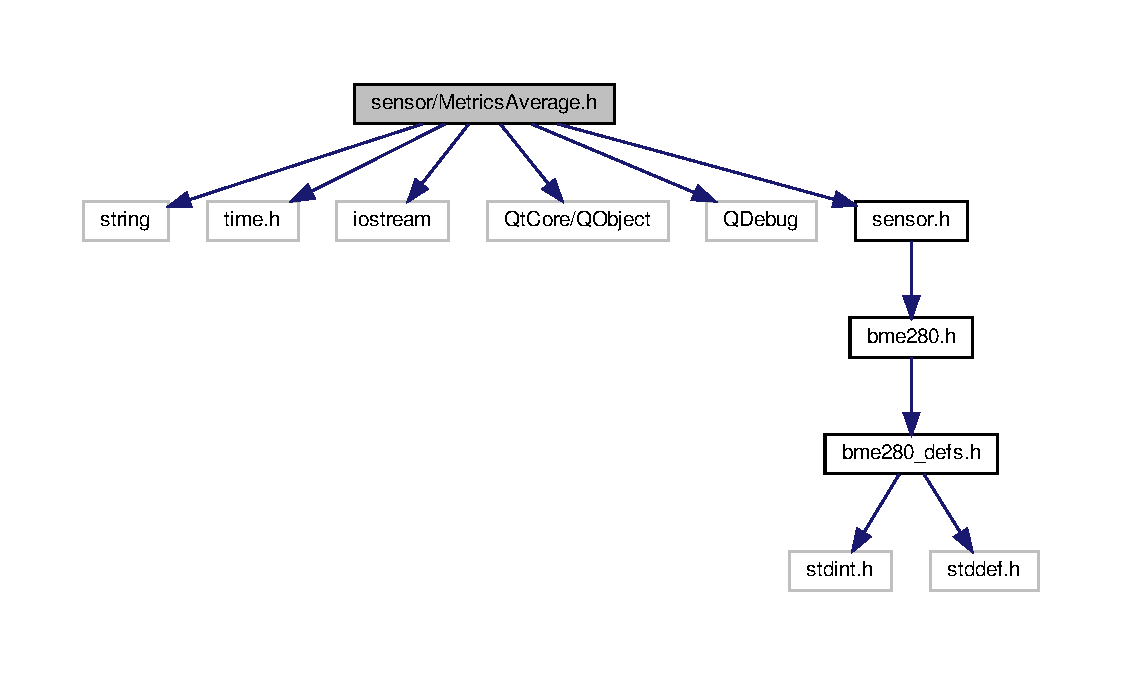
\includegraphics[width=350pt]{_metrics_average_8h__incl}
\end{center}
\end{figure}
This graph shows which files directly or indirectly include this file\+:
\nopagebreak
\begin{figure}[H]
\begin{center}
\leavevmode
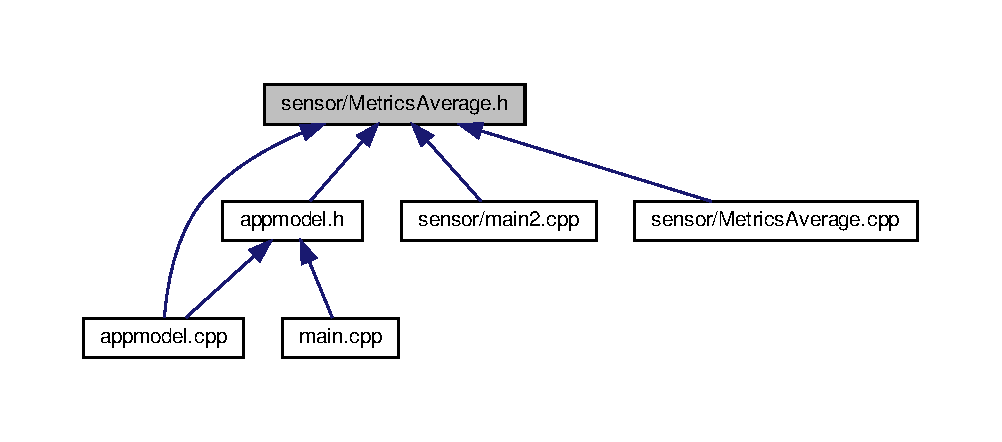
\includegraphics[width=350pt]{_metrics_average_8h__dep__incl}
\end{center}
\end{figure}
\subsection*{Classes}
\begin{DoxyCompactItemize}
\item 
struct \hyperlink{structdatatab}{datatab}
\item 
class \hyperlink{class_metrics_average}{Metrics\+Average}
\end{DoxyCompactItemize}
\subsection*{Functions}
\begin{DoxyCompactItemize}
\item 
int \hyperlink{_metrics_average_8h_a66e7e3e2a1c559ad0cf86f730b9a5549}{rounded} (float x)
\end{DoxyCompactItemize}


\subsection{Function Documentation}
\mbox{\Hypertarget{_metrics_average_8h_a66e7e3e2a1c559ad0cf86f730b9a5549}\label{_metrics_average_8h_a66e7e3e2a1c559ad0cf86f730b9a5549}} 
\index{Metrics\+Average.\+h@{Metrics\+Average.\+h}!rounded@{rounded}}
\index{rounded@{rounded}!Metrics\+Average.\+h@{Metrics\+Average.\+h}}
\subsubsection{\texorpdfstring{rounded()}{rounded()}}
{\footnotesize\ttfamily int rounded (\begin{DoxyParamCaption}\item[{float}]{x }\end{DoxyParamCaption})}


\hypertarget{sensor_8c}{}\section{sensor/sensor.c File Reference}
\label{sensor_8c}\index{sensor/sensor.\+c@{sensor/sensor.\+c}}
{\ttfamily \#include \char`\"{}bme280.\+h\char`\"{}}\newline
{\ttfamily \#include \char`\"{}sensor.\+h\char`\"{}}\newline
{\ttfamily \#include $<$time.\+h$>$}\newline
{\ttfamily \#include $<$stdio.\+h$>$}\newline
{\ttfamily \#include $<$unistd.\+h$>$}\newline
{\ttfamily \#include $<$wiring\+Pi.\+h$>$}\newline
{\ttfamily \#include $<$wiring\+Pi\+S\+P\+I.\+h$>$}\newline
{\ttfamily \#include $<$string.\+h$>$}\newline
{\ttfamily \#include $<$stdlib.\+h$>$}\newline
{\ttfamily \#include $<$linux/i2c-\/dev.\+h$>$}\newline
{\ttfamily \#include $<$sys/ioctl.\+h$>$}\newline
{\ttfamily \#include $<$sys/types.\+h$>$}\newline
{\ttfamily \#include $<$fcntl.\+h$>$}\newline
Include dependency graph for sensor.\+c\+:
\nopagebreak
\begin{figure}[H]
\begin{center}
\leavevmode
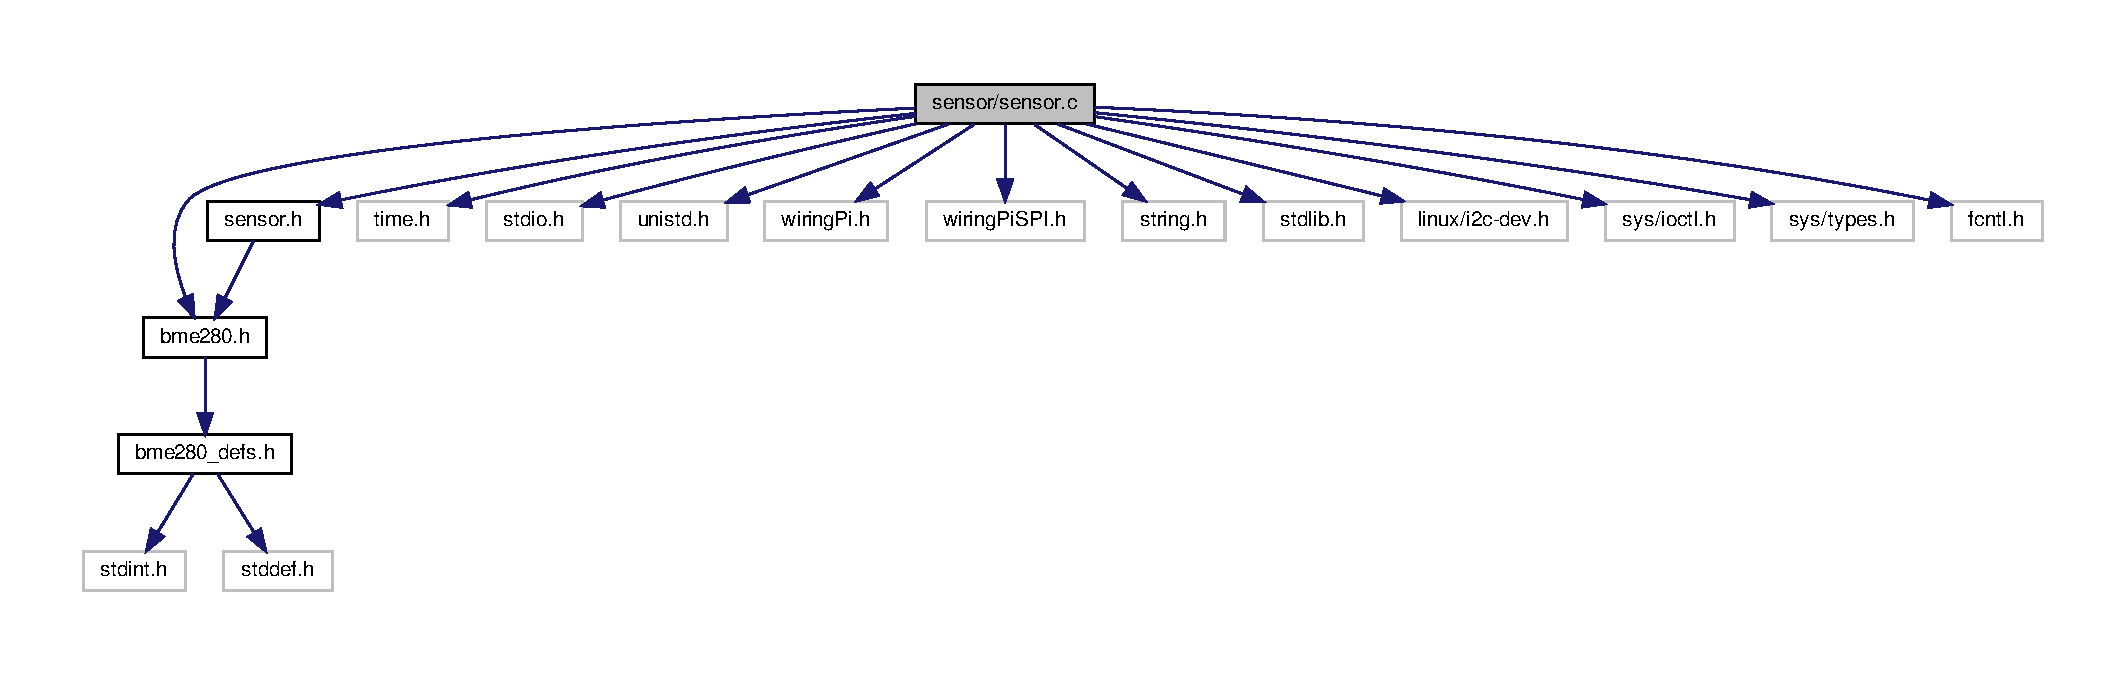
\includegraphics[width=350pt]{sensor_8c__incl}
\end{center}
\end{figure}
\subsection*{Macros}
\begin{DoxyCompactItemize}
\item 
\#define \hyperlink{sensor_8c_ab3f5e0244ce96783f08622c42900b0d9}{channel}~0
\item 
\#define \hyperlink{sensor_8c_a9518a1732e8d5fd66e8a87af770f7bd6}{U\+S\+E\+S\+P\+I\+S\+I\+N\+G\+L\+E\+R\+E\+A\+D\+W\+R\+I\+TE}~0
\item 
\#define \hyperlink{sensor_8c_a02b41100a6327246594b35ed0addb75a}{U\+S\+E\+I\+IC}~1
\item 
\#define \hyperlink{sensor_8c_aae5a5911585681181d49ef77ea110c87}{I\+I\+C\+\_\+\+Dev}~\char`\"{}/dev/i2c-\/1\char`\"{}
\end{DoxyCompactItemize}
\subsection*{Functions}
\begin{DoxyCompactItemize}
\item 
void \hyperlink{sensor_8c_adc86d5995b888a6f4ef7dd5647b94f8f}{user\+\_\+delay\+\_\+ms} (uint32\+\_\+t period)
\item 
int8\+\_\+t \hyperlink{sensor_8c_a61d05d759826396913c31963c102ed66}{user\+\_\+i2c\+\_\+read} (uint8\+\_\+t id, uint8\+\_\+t reg\+\_\+addr, uint8\+\_\+t $\ast$\hyperlink{structdata}{data}, uint16\+\_\+t len)
\item 
int8\+\_\+t \hyperlink{sensor_8c_af8c157ca16fed243ea76c8a1155e8afd}{user\+\_\+i2c\+\_\+write} (uint8\+\_\+t id, uint8\+\_\+t reg\+\_\+addr, uint8\+\_\+t $\ast$\hyperlink{structdata}{data}, uint16\+\_\+t len)
\item 
void \hyperlink{sensor_8c_ac1e8e819dc312cb84abad861e72ea7c4}{print\+\_\+sensor\+\_\+data} (struct \hyperlink{structbme280__data}{bme280\+\_\+data} $\ast$comp\+\_\+data)
\item 
int8\+\_\+t \hyperlink{sensor_8c_a0e934b3f8361dee99aff98fdfa3b55b3}{init\+Sensor} (struct \hyperlink{structbme280__dev}{bme280\+\_\+dev} $\ast$dev)
\item 
struct \hyperlink{structdata}{data} \hyperlink{sensor_8c_adfc1360298a56db6aa43338408f523ba}{refresh\+Sensor} (struct \hyperlink{structbme280__dev}{bme280\+\_\+dev} $\ast$dev)
\end{DoxyCompactItemize}
\subsection*{Variables}
\begin{DoxyCompactItemize}
\item 
int \hyperlink{sensor_8c_a6f8059414f0228f0256115e024eeed4b}{fd}
\end{DoxyCompactItemize}


\subsection{Macro Definition Documentation}
\mbox{\Hypertarget{sensor_8c_ab3f5e0244ce96783f08622c42900b0d9}\label{sensor_8c_ab3f5e0244ce96783f08622c42900b0d9}} 
\index{sensor.\+c@{sensor.\+c}!channel@{channel}}
\index{channel@{channel}!sensor.\+c@{sensor.\+c}}
\subsubsection{\texorpdfstring{channel}{channel}}
{\footnotesize\ttfamily \#define channel~0}

\mbox{\Hypertarget{sensor_8c_aae5a5911585681181d49ef77ea110c87}\label{sensor_8c_aae5a5911585681181d49ef77ea110c87}} 
\index{sensor.\+c@{sensor.\+c}!I\+I\+C\+\_\+\+Dev@{I\+I\+C\+\_\+\+Dev}}
\index{I\+I\+C\+\_\+\+Dev@{I\+I\+C\+\_\+\+Dev}!sensor.\+c@{sensor.\+c}}
\subsubsection{\texorpdfstring{I\+I\+C\+\_\+\+Dev}{IIC\_Dev}}
{\footnotesize\ttfamily \#define I\+I\+C\+\_\+\+Dev~\char`\"{}/dev/i2c-\/1\char`\"{}}

\mbox{\Hypertarget{sensor_8c_a02b41100a6327246594b35ed0addb75a}\label{sensor_8c_a02b41100a6327246594b35ed0addb75a}} 
\index{sensor.\+c@{sensor.\+c}!U\+S\+E\+I\+IC@{U\+S\+E\+I\+IC}}
\index{U\+S\+E\+I\+IC@{U\+S\+E\+I\+IC}!sensor.\+c@{sensor.\+c}}
\subsubsection{\texorpdfstring{U\+S\+E\+I\+IC}{USEIIC}}
{\footnotesize\ttfamily \#define U\+S\+E\+I\+IC~1}

\mbox{\Hypertarget{sensor_8c_a9518a1732e8d5fd66e8a87af770f7bd6}\label{sensor_8c_a9518a1732e8d5fd66e8a87af770f7bd6}} 
\index{sensor.\+c@{sensor.\+c}!U\+S\+E\+S\+P\+I\+S\+I\+N\+G\+L\+E\+R\+E\+A\+D\+W\+R\+I\+TE@{U\+S\+E\+S\+P\+I\+S\+I\+N\+G\+L\+E\+R\+E\+A\+D\+W\+R\+I\+TE}}
\index{U\+S\+E\+S\+P\+I\+S\+I\+N\+G\+L\+E\+R\+E\+A\+D\+W\+R\+I\+TE@{U\+S\+E\+S\+P\+I\+S\+I\+N\+G\+L\+E\+R\+E\+A\+D\+W\+R\+I\+TE}!sensor.\+c@{sensor.\+c}}
\subsubsection{\texorpdfstring{U\+S\+E\+S\+P\+I\+S\+I\+N\+G\+L\+E\+R\+E\+A\+D\+W\+R\+I\+TE}{USESPISINGLEREADWRITE}}
{\footnotesize\ttfamily \#define U\+S\+E\+S\+P\+I\+S\+I\+N\+G\+L\+E\+R\+E\+A\+D\+W\+R\+I\+TE~0}



\subsection{Function Documentation}
\mbox{\Hypertarget{sensor_8c_a0e934b3f8361dee99aff98fdfa3b55b3}\label{sensor_8c_a0e934b3f8361dee99aff98fdfa3b55b3}} 
\index{sensor.\+c@{sensor.\+c}!init\+Sensor@{init\+Sensor}}
\index{init\+Sensor@{init\+Sensor}!sensor.\+c@{sensor.\+c}}
\subsubsection{\texorpdfstring{init\+Sensor()}{initSensor()}}
{\footnotesize\ttfamily int8\+\_\+t init\+Sensor (\begin{DoxyParamCaption}\item[{struct \hyperlink{structbme280__dev}{bme280\+\_\+dev} $\ast$}]{dev }\end{DoxyParamCaption})}

\mbox{\Hypertarget{sensor_8c_ac1e8e819dc312cb84abad861e72ea7c4}\label{sensor_8c_ac1e8e819dc312cb84abad861e72ea7c4}} 
\index{sensor.\+c@{sensor.\+c}!print\+\_\+sensor\+\_\+data@{print\+\_\+sensor\+\_\+data}}
\index{print\+\_\+sensor\+\_\+data@{print\+\_\+sensor\+\_\+data}!sensor.\+c@{sensor.\+c}}
\subsubsection{\texorpdfstring{print\+\_\+sensor\+\_\+data()}{print\_sensor\_data()}}
{\footnotesize\ttfamily void print\+\_\+sensor\+\_\+data (\begin{DoxyParamCaption}\item[{struct \hyperlink{structbme280__data}{bme280\+\_\+data} $\ast$}]{comp\+\_\+data }\end{DoxyParamCaption})}

\mbox{\Hypertarget{sensor_8c_adfc1360298a56db6aa43338408f523ba}\label{sensor_8c_adfc1360298a56db6aa43338408f523ba}} 
\index{sensor.\+c@{sensor.\+c}!refresh\+Sensor@{refresh\+Sensor}}
\index{refresh\+Sensor@{refresh\+Sensor}!sensor.\+c@{sensor.\+c}}
\subsubsection{\texorpdfstring{refresh\+Sensor()}{refreshSensor()}}
{\footnotesize\ttfamily struct \hyperlink{structdata}{data} refresh\+Sensor (\begin{DoxyParamCaption}\item[{struct \hyperlink{structbme280__dev}{bme280\+\_\+dev} $\ast$}]{dev }\end{DoxyParamCaption})}

\mbox{\Hypertarget{sensor_8c_adc86d5995b888a6f4ef7dd5647b94f8f}\label{sensor_8c_adc86d5995b888a6f4ef7dd5647b94f8f}} 
\index{sensor.\+c@{sensor.\+c}!user\+\_\+delay\+\_\+ms@{user\+\_\+delay\+\_\+ms}}
\index{user\+\_\+delay\+\_\+ms@{user\+\_\+delay\+\_\+ms}!sensor.\+c@{sensor.\+c}}
\subsubsection{\texorpdfstring{user\+\_\+delay\+\_\+ms()}{user\_delay\_ms()}}
{\footnotesize\ttfamily void user\+\_\+delay\+\_\+ms (\begin{DoxyParamCaption}\item[{uint32\+\_\+t}]{period }\end{DoxyParamCaption})}

\mbox{\Hypertarget{sensor_8c_a61d05d759826396913c31963c102ed66}\label{sensor_8c_a61d05d759826396913c31963c102ed66}} 
\index{sensor.\+c@{sensor.\+c}!user\+\_\+i2c\+\_\+read@{user\+\_\+i2c\+\_\+read}}
\index{user\+\_\+i2c\+\_\+read@{user\+\_\+i2c\+\_\+read}!sensor.\+c@{sensor.\+c}}
\subsubsection{\texorpdfstring{user\+\_\+i2c\+\_\+read()}{user\_i2c\_read()}}
{\footnotesize\ttfamily int8\+\_\+t user\+\_\+i2c\+\_\+read (\begin{DoxyParamCaption}\item[{uint8\+\_\+t}]{id,  }\item[{uint8\+\_\+t}]{reg\+\_\+addr,  }\item[{uint8\+\_\+t $\ast$}]{data,  }\item[{uint16\+\_\+t}]{len }\end{DoxyParamCaption})}

\mbox{\Hypertarget{sensor_8c_af8c157ca16fed243ea76c8a1155e8afd}\label{sensor_8c_af8c157ca16fed243ea76c8a1155e8afd}} 
\index{sensor.\+c@{sensor.\+c}!user\+\_\+i2c\+\_\+write@{user\+\_\+i2c\+\_\+write}}
\index{user\+\_\+i2c\+\_\+write@{user\+\_\+i2c\+\_\+write}!sensor.\+c@{sensor.\+c}}
\subsubsection{\texorpdfstring{user\+\_\+i2c\+\_\+write()}{user\_i2c\_write()}}
{\footnotesize\ttfamily int8\+\_\+t user\+\_\+i2c\+\_\+write (\begin{DoxyParamCaption}\item[{uint8\+\_\+t}]{id,  }\item[{uint8\+\_\+t}]{reg\+\_\+addr,  }\item[{uint8\+\_\+t $\ast$}]{data,  }\item[{uint16\+\_\+t}]{len }\end{DoxyParamCaption})}



\subsection{Variable Documentation}
\mbox{\Hypertarget{sensor_8c_a6f8059414f0228f0256115e024eeed4b}\label{sensor_8c_a6f8059414f0228f0256115e024eeed4b}} 
\index{sensor.\+c@{sensor.\+c}!fd@{fd}}
\index{fd@{fd}!sensor.\+c@{sensor.\+c}}
\subsubsection{\texorpdfstring{fd}{fd}}
{\footnotesize\ttfamily int fd}


\hypertarget{sensor_8h}{}\section{sensor/sensor.h File Reference}
\label{sensor_8h}\index{sensor/sensor.\+h@{sensor/sensor.\+h}}
{\ttfamily \#include \char`\"{}bme280.\+h\char`\"{}}\newline
Include dependency graph for sensor.\+h\+:
\nopagebreak
\begin{figure}[H]
\begin{center}
\leavevmode
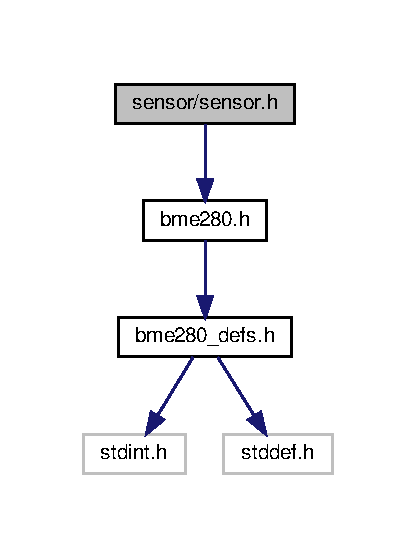
\includegraphics[width=200pt]{sensor_8h__incl}
\end{center}
\end{figure}
This graph shows which files directly or indirectly include this file\+:
\nopagebreak
\begin{figure}[H]
\begin{center}
\leavevmode
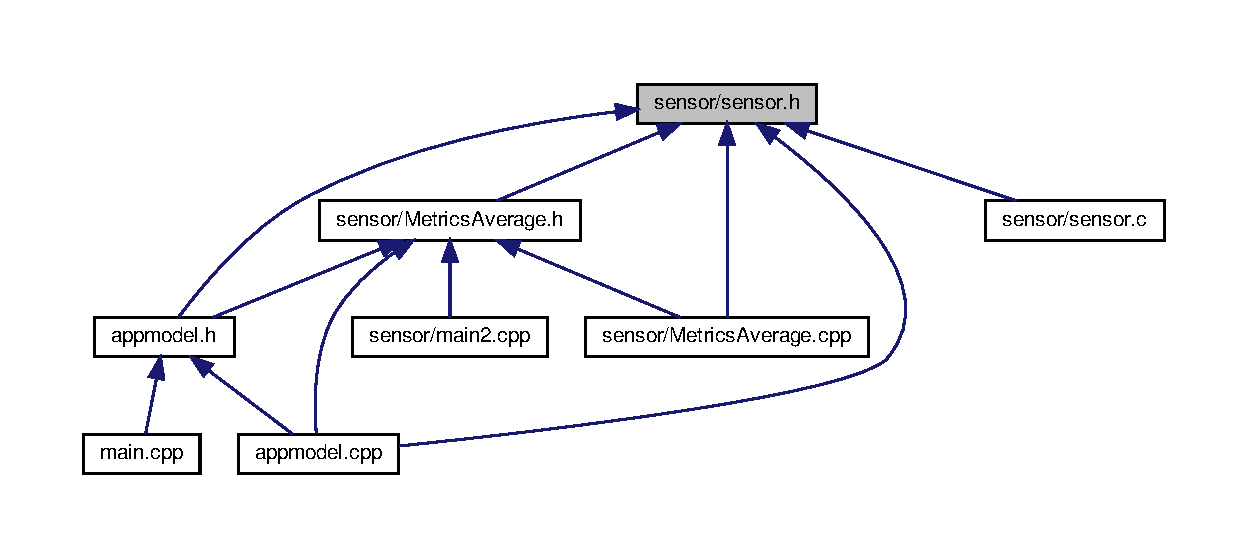
\includegraphics[width=350pt]{sensor_8h__dep__incl}
\end{center}
\end{figure}
\subsection*{Classes}
\begin{DoxyCompactItemize}
\item 
struct \hyperlink{structdata}{data}
\end{DoxyCompactItemize}
\subsection*{Functions}
\begin{DoxyCompactItemize}
\item 
int8\+\_\+t \hyperlink{sensor_8h_a0e934b3f8361dee99aff98fdfa3b55b3}{init\+Sensor} (struct \hyperlink{structbme280__dev}{bme280\+\_\+dev} $\ast$dev)
\item 
struct \hyperlink{structdata}{data} \hyperlink{sensor_8h_adfc1360298a56db6aa43338408f523ba}{refresh\+Sensor} (struct \hyperlink{structbme280__dev}{bme280\+\_\+dev} $\ast$dev)
\end{DoxyCompactItemize}


\subsection{Function Documentation}
\mbox{\Hypertarget{sensor_8h_a0e934b3f8361dee99aff98fdfa3b55b3}\label{sensor_8h_a0e934b3f8361dee99aff98fdfa3b55b3}} 
\index{sensor.\+h@{sensor.\+h}!init\+Sensor@{init\+Sensor}}
\index{init\+Sensor@{init\+Sensor}!sensor.\+h@{sensor.\+h}}
\subsubsection{\texorpdfstring{init\+Sensor()}{initSensor()}}
{\footnotesize\ttfamily int8\+\_\+t init\+Sensor (\begin{DoxyParamCaption}\item[{struct \hyperlink{structbme280__dev}{bme280\+\_\+dev} $\ast$}]{dev }\end{DoxyParamCaption})}

\mbox{\Hypertarget{sensor_8h_adfc1360298a56db6aa43338408f523ba}\label{sensor_8h_adfc1360298a56db6aa43338408f523ba}} 
\index{sensor.\+h@{sensor.\+h}!refresh\+Sensor@{refresh\+Sensor}}
\index{refresh\+Sensor@{refresh\+Sensor}!sensor.\+h@{sensor.\+h}}
\subsubsection{\texorpdfstring{refresh\+Sensor()}{refreshSensor()}}
{\footnotesize\ttfamily struct \hyperlink{structdata}{data} refresh\+Sensor (\begin{DoxyParamCaption}\item[{struct \hyperlink{structbme280__dev}{bme280\+\_\+dev} $\ast$}]{dev }\end{DoxyParamCaption})}


\hypertarget{_zambretti_8cpp}{}\section{zambretti/\+Zambretti.cpp File Reference}
\label{_zambretti_8cpp}\index{zambretti/\+Zambretti.\+cpp@{zambretti/\+Zambretti.\+cpp}}
{\ttfamily \#include \char`\"{}Zambretti.\+h\char`\"{}}\newline
{\ttfamily \#include $<$string$>$}\newline
{\ttfamily \#include $<$iostream$>$}\newline
{\ttfamily \#include $<$time.\+h$>$}\newline
{\ttfamily \#include $<$float.\+h$>$}\newline
Include dependency graph for Zambretti.\+cpp\+:
\nopagebreak
\begin{figure}[H]
\begin{center}
\leavevmode
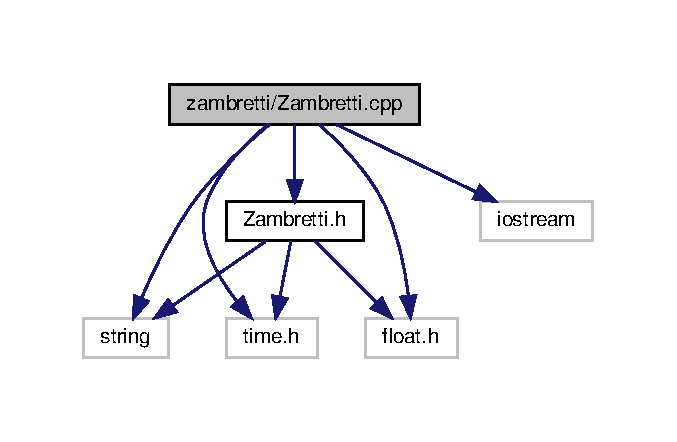
\includegraphics[width=325pt]{_zambretti_8cpp__incl}
\end{center}
\end{figure}
\subsection*{Functions}
\begin{DoxyCompactItemize}
\item 
int \hyperlink{_zambretti_8cpp_a66e7e3e2a1c559ad0cf86f730b9a5549}{rounded} (float x)
\end{DoxyCompactItemize}


\subsection{Function Documentation}
\mbox{\Hypertarget{_zambretti_8cpp_a66e7e3e2a1c559ad0cf86f730b9a5549}\label{_zambretti_8cpp_a66e7e3e2a1c559ad0cf86f730b9a5549}} 
\index{Zambretti.\+cpp@{Zambretti.\+cpp}!rounded@{rounded}}
\index{rounded@{rounded}!Zambretti.\+cpp@{Zambretti.\+cpp}}
\subsubsection{\texorpdfstring{rounded()}{rounded()}}
{\footnotesize\ttfamily int rounded (\begin{DoxyParamCaption}\item[{float}]{x }\end{DoxyParamCaption})}


\hypertarget{_zambretti_8h}{}\section{zambretti/\+Zambretti.h File Reference}
\label{_zambretti_8h}\index{zambretti/\+Zambretti.\+h@{zambretti/\+Zambretti.\+h}}
{\ttfamily \#include $<$string$>$}\newline
{\ttfamily \#include $<$time.\+h$>$}\newline
{\ttfamily \#include $<$float.\+h$>$}\newline
Include dependency graph for Zambretti.\+h\+:
\nopagebreak
\begin{figure}[H]
\begin{center}
\leavevmode
\includegraphics[width=246pt]{_zambretti_8h__incl}
\end{center}
\end{figure}
This graph shows which files directly or indirectly include this file\+:
\nopagebreak
\begin{figure}[H]
\begin{center}
\leavevmode
\includegraphics[width=350pt]{_zambretti_8h__dep__incl}
\end{center}
\end{figure}
\subsection*{Classes}
\begin{DoxyCompactItemize}
\item 
class \hyperlink{class_zambretti}{Zambretti}
\end{DoxyCompactItemize}

%--- End generated contents ---

% Index
\backmatter
\newpage
\phantomsection
\clearemptydoublepage
\addcontentsline{toc}{chapter}{Index}
\printindex

\end{document}
